\documentclass{csnotes}
\usepackage{xcolor}
\usepackage[italian]{babel}
\usepackage{geometry}
\usepackage{graphicx}
\usepackage{xcolor}
\usepackage{hyperref}
\usepackage{listings}
\usepackage{booktabs}
\usepackage{amsmath}
\usepackage{hyperref}
\usepackage{tikz}
\usetikzlibrary{arrows.meta}
\usepackage{pgfplots}
\usepackage{placeins}
\usepackage{caption}
\pgfplotsset{compat=1.18}
\usepackage{graphicx}
\definecolor{primary}{rgb}{0.12, 0.28, 0.52}
\definecolor{accent}{rgb}{0.8, 0.2, 0.2}


\lstdefinelanguage{turtle}{
  morekeywords={@prefix, @base},
  morecomment=[l]{\#},
  morestring=[b]",
  sensitive=true
}
\lstset{
  language=turtle,
  basicstyle=\small\ttfamily,
  keywordstyle=\color{purple}\bfseries,
  stringstyle=\color{teal},
  commentstyle=\color{gray}\itshape,
  numbers=none,
  frame=single,
  rulecolor=\color{lightgray},
  backgroundcolor=\color{gray!5},
  breaklines=true,
  tabsize=2,
  showstringspaces=false
}
\geometry{
    top=2cm,
    bottom=2cm,
    left=2cm,
    right=2cm
}
% Document meta
\title{Ricerca Operativa}
\author{Giuliano Savino}
\date{\today}

% Title page info
\university{Università Degli Studi Di Napoli Federico II}
\department{Dipartimento Di Ingegneria Elettrica \\ e Delle Tecnologie Dell'Informazione}
\course{Corso Di Laurea Magistrale In Informatica}
\subject{Ricerca Operativa}
\academicyear{Academic Year 2026/2027}

\begin{document}
\begin{titlepage}
\thispagestyle{empty}
\centering

% Colori del frontespizio
\definecolor{coverblue}{RGB}{31,71,133}
\definecolor{coverlight}{RGB}{235,242,250}
\definecolor{coveraccent}{RGB}{204,51,51}

% Intestazione
{\large\bfseries\color{coverblue}
Università degli Studi di Napoli Federico II\par}

\vspace{0.35cm}

{\small
Dipartimento di Ingegneria Elettrica\\
e delle Tecnologie dell'Informazione\par}

\vspace{0.25cm}

{\small
Corso di Laurea Magistrale in Informatica\par}

\vspace{0.7cm}

{\color{coverblue}\rule{\textwidth}{1.1pt}}

\vfill

% Titolo
{\small\bfseries\color{coverblue}
A P P U N T I\par}

\vspace{0.45cm}

{\fontsize{38}{44}\selectfont\bfseries
\color{coverblue}
Ricerca\\[0.1cm]
Operativa\par}

\vspace{0.5cm}

{\large\color{black!55}
Modelli, metodi e ottimizzazione\par}

\vspace{1cm}

% Illustrazione vettoriale:
% regione ammissibile e soluzione ottima
\begin{tikzpicture}[
    x=1.15cm,
    y=1.15cm,
    >=Stealth,
    line cap=round,
    line join=round,
    font=\small
]
    % Griglia leggera
    \draw[
        step=0.5,
        coverblue!7,
        very thin
    ] (0,0) grid (5.3,4);

    % Regione ammissibile:
    % x_1 >= 0, x_2 >= 0,
    % x_1 <= 4, x_2 <= 3, x_1 + x_2 <= 5
    \fill[coverlight]
        (0,0) -- (4,0) -- (4,1) --
        (2,3) -- (0,3) -- cycle;

    % Rette associate ai vincoli
    \draw[coverblue!25, thin]
        (1.2,3.8) -- (4.8,0.2);
    \draw[coverblue!25, thin]
        (0,3) -- (5.1,3);
    \draw[coverblue!25, thin]
        (4,0) -- (4,3.8);

    % Contorno della regione
    \draw[coverblue, very thick]
        (0,0) -- (4,0) -- (4,1) --
        (2,3) -- (0,3) -- cycle;

    % Assi
    \draw[->, black!50, thin]
        (-0.2,0) -- (5.55,0)
        node[right] {$x_1$};

    \draw[->, black!50, thin]
        (0,-0.2) -- (0,4.2)
        node[above] {$x_2$};

    % Vertici
    \foreach \p in {(0,0),(4,0),(2,3),(0,3)}
        \fill[coverblue] \p circle (2pt);

    % Etichetta interna
    \node[
        align=center,
        text=coverblue
    ] at (1.65,1.05)
        {Regione\\ammissibile};

    % Direzione di miglioramento per max 2x_1 + x_2
    \draw[
        ->,
        coveraccent,
        thick
    ] (2.0,1.65) -- (3.0,2.15);

    % Retta di livello ottima: 2x_1 + x_2 = 9
    \draw[
        coveraccent!75,
        dashed,
        thick
    ] (2.7,3.6) -- (4.5,0);

    % Soluzione ottima
    \fill[coveraccent!12]
        (4,1) circle (0.19);

    \fill[coveraccent]
        (4,1) circle (3pt);

    \draw[coveraccent!65, thin]
        (4.12,1.12) -- (4.55,1.65);

    \node[
        anchor=west,
        text=coveraccent,
        font=\small\bfseries,
        align=left
    ] at (4.55,1.65)
        {Soluzione\\ottima};

\end{tikzpicture}

\vspace{0.45cm}



\vfill

% Autore
{\small\color{black!55}A cura di\par}

\vspace{0.15cm}

{\Large\bfseries\color{coverblue}
Giuliano Savino\par}

\vspace{0.9cm}

{\color{coverblue}\rule{\textwidth}{0.5pt}}

\vspace{0.35cm}

{\small\color{black!55}
Anno Accademico 2026/2027\par}

\end{titlepage}

\tableofcontents
\newpage

\tableofcontents
\newpage
\chapter{Preambolo}
\section{Rango di una matrice}
Consideriamo una matrice $A \in \mathbb{R} ^ {m \times n}$
\begin{definition}{Rango di una Matrice}
    Il rango di una matrice indica il numero di righe (o colonne, dipende da che notazione usiamo), lineramente indipendenti.
\end{definition}
\begin{proposition}{Rango Massimo di una Matrice}
Data una matrice \(A \in \mathbb{R}^{m \times n}\), il suo rango massimo è
\[
\boxed{\operatorname{rank}(A) \leq \min(m,n)}
\]
\end{proposition}
Perchè intuitivamente si ha questa proprietà?
Immagina avere una matrice dove i vettori sono sulle righe:
\[
A=
\begin{pmatrix}
1&0\\
0&1\\
1&1
\end{pmatrix}
\]
In questa matrice il rango massimo è 2, questo perchè in $\mathbb{R}^2$, al massimo due vettori possono essere lineramente indipendenti, se ne aggiungo un terzo, questo sarà sicuramamente combinazione lineare degli altri due. \\
Consideriamo questa altra matrice:
\[
A=
\begin{pmatrix}
1&0&1\\
0&1&0
\end{pmatrix}
\]
In questa matrice il rango massimo è sempre 2, questo perchè ci sono due vettori sulle righe.


\subsection{Cosa succede quando il rango è massimo ?}

Sia $R \in \mathbb{R}^{N \times M}$ una matrice con $N$ righe e $M$ colonne.

Il \textbf{rango} di una matrice è definito come il massimo numero di righe (o, equivalentemente, di colonne) linearmente indipendenti.

Per qualsiasi matrice vale la seguente proprietà:

\[
    \operatorname{rank}(R) \leq \min\{N,M\}.
\]

Il rango non può quindi superare il numero di righe né il numero di colonne della matrice.

Si dice che una matrice ha \textbf{rango massimo} (o \textit{full rank}) quando:

\[
    \boxed{\operatorname{rank}(R) = \min\{N,M\}.}
\]

In questo caso, la matrice contiene il massimo numero possibile di vettori linearmente indipendenti.

\paragraph{Caso 1: $N < M$ (più colonne che righe)}

Se la matrice ha più colonne che righe, il rango massimo è:

\[
    \operatorname{rank}(R) = N.
\]

Questo implica che:
\begin{itemize}
    \item Le $N$ righe sono tutte linearmente indipendenti.
    \item Esistono $N$ colonne linearmente indipendenti.
    \item Le $M$ colonne non possono essere tutte linearmente indipendenti, poiché $M > N$ e ciascuna colonna appartiene a $\mathbb{R}^N$.
\end{itemize}

Ad esempio, per una matrice $R \in \mathbb{R}^{3 \times 5}$, il rango massimo è $3$. Le tre righe possono essere tutte linearmente indipendenti, mentre tra le cinque colonne al massimo tre possono esserlo.

\paragraph{Caso 2: $N > M$ (più righe che colonne)}

Se la matrice ha più righe che colonne, il rango massimo è:

\[
    \operatorname{rank}(R) = M.
\]

Questo implica che:
\begin{itemize}
    \item Le $M$ colonne sono tutte linearmente indipendenti.
    \item Esistono $M$ righe linearmente indipendenti.
    \item Le $N$ righe non possono essere tutte linearmente indipendenti, poiché $N > M$ e ciascuna riga appartiene a $\mathbb{R}^M$.
\end{itemize}

\paragraph{Caso 3: $N = M$ (matrice quadrata)}

Se la matrice è quadrata, il rango massimo è:

\[
    \operatorname{rank}(R) = N = M.
\]

In questo caso:
\begin{itemize}
    \item Tutte le righe sono linearmente indipendenti.
    \item Tutte le colonne sono linearmente indipendenti.
    \item La matrice è invertibile, ossia esiste $R^{-1}$.
    \item Il determinante è diverso da zero: $\det(R) \neq 0$.
\end{itemize}

\paragraph{Interpretazione geometrica}

Le colonne di una matrice $R \in \mathbb{R}^{N \times M}$ sono vettori appartenenti allo spazio $\mathbb{R}^{N}$, mentre le righe sono vettori appartenenti a $\mathbb{R}^{M}$.

In uno spazio vettoriale di dimensione $d$, non possono esistere più di $d$ vettori linearmente indipendenti.

Pertanto, se $M > N$, le $M$ colonne di $R$ non potranno mai essere tutte linearmente indipendenti, indipendentemente dai valori contenuti nella matrice.

\paragraph{Osservazione fondamentale}

Avere rango massimo \textbf{non significa necessariamente che tutte le righe e tutte le colonne siano linearmente indipendenti}.

Significa, invece, che la matrice possiede il massimo numero di vettori linearmente indipendenti consentito dalle sue dimensioni:

\[
    \boxed{\operatorname{rank}(R) = \min\{N,M\}.}
\]

Solo nel caso di una matrice quadrata a rango massimo si può affermare che tutte le righe e tutte le colonne sono contemporaneamente linearmente indipendenti.


 \section{Linearmente Indipendenza}

Due o più vettori si dicono **linearmente indipendenti** quando nessuno di essi può essere espresso come combinazione lineare degli altri. Nel caso particolare di due vettori, questo significa che uno non può essere ottenuto moltiplicando l'altro per uno scalare.

Al contrario, due o più vettori si dicono **linearmente dipendenti** quando almeno uno di essi può essere espresso come combinazione lineare degli altri.

\subsection{Interpretazione geometrica nel piano}

Consideriamo due vettori appartenenti allo spazio \(\mathbb{R}^2\). Possiamo interpretarli geometricamente come frecce che partono dall'origine del piano cartesiano e terminano nei punti individuati dalle loro coordinate.

\subsubsection{Vettori linearmente indipendenti}

Consideriamo i seguenti vettori:

\[
v_1 =
\begin{pmatrix}
1\\
0
\end{pmatrix},
\qquad
v_2 =
\begin{pmatrix}
0\\
1
\end{pmatrix}.
\]

Il vettore \(v_1\) è diretto orizzontalmente verso destra, mentre il vettore \(v_2\) è diretto verticalmente verso l'alto. I due vettori hanno quindi direzioni differenti e non appartengono alla stessa retta passante per l'origine.

Per verificare che siano linearmente indipendenti, consideriamo l'equazione:

\[
\alpha v_1+\beta v_2=
\begin{pmatrix}
0\\
0
\end{pmatrix}.
\]

Sostituendo i vettori otteniamo:

\[
\alpha
\begin{pmatrix}
1\\
0
\end{pmatrix}
+
\beta
\begin{pmatrix}
0\\
1
\end{pmatrix}
=
\begin{pmatrix}
0\\
0
\end{pmatrix}.
\]

Da cui segue:

\[
\begin{cases}
\alpha=0\\
\beta=0
\end{cases}
\]

L'unica combinazione lineare che restituisce il vettore nullo è quindi quella in cui entrambi i coefficienti sono nulli. I due vettori sono pertanto linearmente indipendenti.

\paragraph{Significato geometrico.}

Due vettori linearmente indipendenti in \(\mathbb{R}^2\) individuano due direzioni distinte. Combinandoli linearmente, possiamo ottenere qualsiasi vettore del piano:

\[
\alpha v_1+\beta v_2
=
\begin{pmatrix}
\alpha\\
\beta
\end{pmatrix}.
\]

Infatti, scegliendo opportunamente i coefficienti \(\alpha\) e \(\beta\), possiamo raggiungere qualsiasi punto del piano cartesiano.

\subsubsection{Vettori linearmente dipendenti}

Consideriamo ora i vettori:

\[
v_1 =
\begin{pmatrix}
1\\
2
\end{pmatrix},
\qquad
v_2 =
\begin{pmatrix}
2\\
4
\end{pmatrix}.
\]

Osserviamo che il secondo vettore è il doppio del primo:

\[
v_2=2v_1.
\]

Pertanto, i due vettori hanno la stessa direzione e appartengono alla medesima retta passante per l'origine.

Per determinare l'equazione di questa retta, interpretiamo i vettori come punti del piano cartesiano.

Il primo vettore individua il punto \(P_1=(1,2)\), mentre il secondo individua il punto \(P_2=(2,4)\).

Entrambi i punti soddisfano la relazione:

\[
\boxed{y=2x}
\]

Infatti:
\begin{itemize}
    \item Per \(P_1=(1,2)\), abbiamo \(2=2\cdot 1\).
    \item Per \(P_2=(2,4)\), abbiamo \(4=2\cdot 2\).
\end{itemize}

La retta \(y=2x\) passa anche per l'origine \((0,0)\), poiché \(0=2\cdot 0\).

\paragraph{Verifica dell'indipendenza lineare.}

Per verificare che i vettori siano linearmente dipendenti, cerchiamo una combinazione lineare che restituisca il vettore nullo con coefficienti non entrambi nulli:

\[
\alpha v_1+\beta v_2=
\begin{pmatrix}
0\\
0
\end{pmatrix}.
\]

Sostituendo:

\[
\alpha
\begin{pmatrix}
1\\
2
\end{pmatrix}
+
\beta
\begin{pmatrix}
2\\
4
\end{pmatrix}
=
\begin{pmatrix}
0\\
0
\end{pmatrix}.
\]

Otteniamo il sistema:

\[
\begin{cases}
\alpha+2\beta=0\\
2\alpha+4\beta=0
\end{cases}
\]

Le due equazioni sono equivalenti. Esistono quindi infinite soluzioni non banali; ad esempio, scegliendo \(\alpha=-2\) e \(\beta=1\), si ottiene:

\[
-2v_1+v_2=
\begin{pmatrix}
0\\
0
\end{pmatrix}.
\]

I due vettori sono dunque linearmente dipendenti.

\paragraph{Significato geometrico.}

Combinando linearmente due vettori dipendenti, possiamo ottenere soltanto vettori appartenenti alla retta che li contiene. Non possiamo generare qualsiasi vettore del piano, perché i due vettori non introducono due direzioni distinte.

\subsection{Riepilogo geometrico}

Nel piano \(\mathbb{R}^2\), per due vettori non entrambi nulli, possiamo riassumere il concetto nel modo seguente:

\begin{itemize}
    \item \textbf{Vettori linearmente indipendenti:} i vettori non appartengono alla stessa retta passante per l'origine. Generano tutto il piano \(\mathbb{R}^2\).
    \item \textbf{Vettori linearmente dipendenti:} i vettori appartengono alla stessa retta passante per l'origine. Generano al massimo una retta.
\end{itemize}

\textbf{Attenzione:} se almeno uno dei vettori è il vettore nullo, i vettori sono linearmente dipendenti. Inoltre, nel caso di due vettori non nulli, essere sulla stessa retta passante per l'origine equivale a essere multipli scalari l'uno dell'altro.

\subsection{Collegamento con le matrici}

Il concetto di indipendenza lineare è utile anche nello studio delle matrici, in particolare nella Ricerca Operativa.

Consideriamo una matrice le cui colonne sono due vettori:

\[
A=
\begin{pmatrix}
1 & 2\\
2 & 4
\end{pmatrix}.
\]

Le colonne sono:

\[
A_1=
\begin{pmatrix}
1\\
2
\end{pmatrix},
\qquad
A_2=
\begin{pmatrix}
2\\
4
\end{pmatrix}.
\]

Poiché \(A_2=2A_1\), le colonne sono linearmente dipendenti e la matrice non ha rango massimo.

Al contrario, se le colonne sono linearmente indipendenti, descrivono direzioni distinte. In particolare, una matrice quadrata \(2\times 2\) ha rango massimo pari a \(2\) se e solo se le sue due colonne sono linearmente indipendenti.

Questo permette di collegare l'interpretazione geometrica dei vettori al concetto di rango di una matrice.



\section{Funzioni Convesse}

\subsection{Definizione Matematica}

Sia $I \subseteq \mathbb{R}$ un intervallo (limitato o illimitato). Una funzione $f: I \to \mathbb{R}$ si dice \textbf{convessa} su $I$ se, per ogni coppia di punti $x_1, x_2 \in I$ e per ogni $t \in [0, 1]$, si ha:
\begin{equation}
    f(t x_1 + (1-t) x_2) \le t f(x_1) + (1-t) f(x_2)
\end{equation}

Se la disuguaglianza vale in senso stretto per ogni $x_1 \neq x_2$ e per ogni $t \in (0, 1)$, ovvero:
\begin{equation}
    f(t x_1 + (1-t) x_2) < t f(x_1) + (1-t) f(x_2)
\end{equation}
la funzione si dice \textbf{strettamente convessa} su $I$.

\newpage

\paragraph{Interpretazione algebrica:} Il punto $x_t = t x_1 + (1-t) x_2$ rappresenta un generico punto compreso nell'intervallo $[x_1, x_2]$. La quantità $t f(x_1) + (1-t) f(x_2)$ rappresenta la quota corrispondente a $x_t$ sulla corda (segmento) che congiunge i punti $(x_1, f(x_1))$ e $(x_2, f(x_2))$.
Invece la quantità $f(t x_1 + (1-t) x_2)$, rappresenta la quota della funzione di un punto compreso nell'intervallo $[x_1, x_2]$.

Si deve avere che la quotà della funzione di un punto compreso nell'intervallo $[x_1, x_2]$, deve essere minore della quota corrispondente al segmento che congiunge $(x_1, f(x_1))$ e $(x_2, f(x_2))$.

\begin{figure}[htbp]
        \centering
        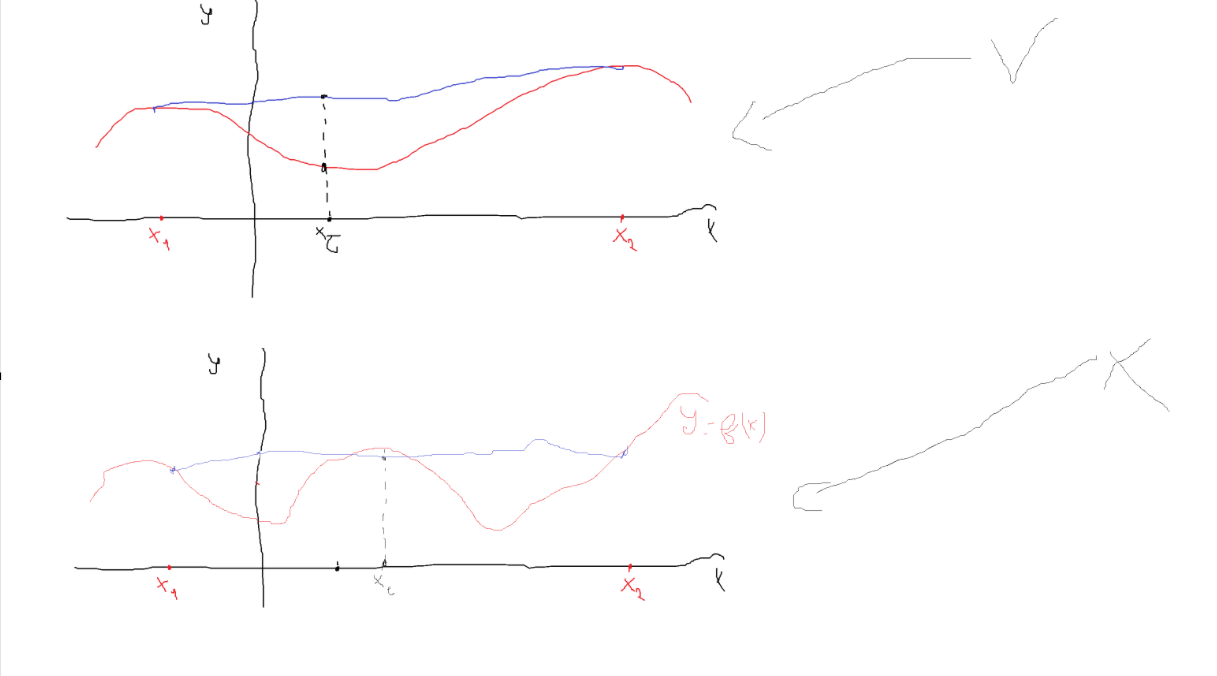
\includegraphics[width=0.8\textwidth]{_files/_images/28.png}
        \caption{Sopra vi è una funzione convessa, sotto no}
        \label{fig:mia_immagine}
\end{figure}
\chapter{Introduzione}
La Ricerca Operativa è la disciplina che studia e mette a punto metodologie ed algoritmi per la risoluzione di problemi di ottimizzazione
\begin{definition}{Problema Ottimizzazione}
    Un problema di ottimizzazione è un problema in cui occorre prendere decisioni sull'uso di risorse disponibili solo in quantità limitate,
    in modo tale da rispettare un dato insieme di vincoli, e da massimizzare il beneficio ottenibile dall'uso delle risorse \textbf{o minimizzare
    il costo totale che ne deriva dall'utilizzo di queste risorse.}
\end{definition}
\begin{example}{Esempio di problema di ottimizzazione}
    Supponiamo che un'azienda produca tavoli e sedie:
    \begin{itemize}
        \item Ogni tavolo richiede 4 ore di lavoro e 2 kg di legno.
        \item Ogni sedia richiede 2 ore di lavoro e 1 kg di legno.
        \item L'azienda dispone di 40 ore di lavoro e 16 kg di legno.
        \item Guadagna 50 € per ogni tavolo e 20 € per ogni sedia.
    \end{itemize}
    Indichiamo con
    \begin{itemize}
        \item x = numero di tavoli prodotti.
        \item y = numero di sedie prodotte.
    \end{itemize}
    Vogliamo massimizzare il profitto
    \begin{center}
        $\max_{x,y} (50x + 20y)$


        soggetto ai vincoli
        $$
        \begin{cases}
        4x + 2y \le 40 & \text{(ore di lavoro)} \\
        2x + y \le 16 & \text{(legno)} \\
        x, y \ge 0
        \end{cases}
        $$
    \end{center}
\end{example}
Quindi un processo decisionale alla base dell'analisi e risoluzione di un problema
di ottimizzazione puo essere scomposto nelle seguenti fasi:
\begin{itemize}
    \item individuazione del problema e delle sue caratteristiche;
    \item costruzione di un modello logico-matematico che lo rappresenti (formulazione degli obiettivi e scelta della variabili di interesse, dette variabili
di decisione, nell'esempio di prima sono x ed y);
    \item determinazione di una o piu soluzioni;
    \item analisi dei risultati ottenuti.
\end{itemize}
\newpage
\section{Classificazione dei problemi di ottimizzazione}
Per definire matematicamente un problema di ottimo, quello che si fa è definire:
\begin{definition}{Insieme ammissibile}
    \begin{center}
        P = \{\text{tutte le soluzioni che rispettano i vincoli del problema}\}
    \end{center}
    P viene chiamato insieme ammissibile e ogni elemento x $\in$ P è \textbf{una soluzione ammissibile}
\end{definition}
\begin{example}{Esempio di Insieme ammissibile}
    Nell'esempio dei tavoli e delle sedie avevamo:
    \begin{center}
        $$
        \begin{cases}
        4x + 2y \le 40 & \text{(ore di lavoro)} \\
        2x + y \le 16 & \text{(legno)} \\
        x, y \ge 0
        \end{cases}
        $$
    \end{center}
    Quindi l'insieme ammissibile è 
    \begin{center}
        $$
        P = \left\{ (x,y) \in \mathbb{R}^2 : 
        \begin{array}{l}
        4x + 2y \le 40 \\
        2x + y \le 16 \\
        x \ge 0, y \ge 0
        \end{array} 
        \right\}
        $$
    \end{center}
\end{example}
\begin{definition}{Funzione Obiettivo}
    Sull'insieme $P$, viene definita una funzione:
    \begin{center}
        $c : P \to \mathbb{R}$
    \end{center}
    Questa funzione associa ad ogni soluzione ammissibile un valore reale:
    \begin{center}
           $x \in P \to c(x) \in \mathbb{R}$
    \end{center}
    Il valore \(c(x)\) rappresenta, a seconda del problema:
    \begin{itemize}
        \item \textbf{un profitto/beneficio}, che vogliamo massimizzare.
        \item \textbf{un costo}, vogliamo minimizzarlo.
    \end{itemize}
\end{definition}
\begin{definition}{Problema di Ottimizzazione}
    Quindi un problema di ottimizzazione può essere scritto semplicemente come:
    \begin{center}
        $\max_{x \in P} c(x)$
    \end{center}
    oppure
    \begin{center}
        $\min_{x \in P} c(x)$
    \end{center}
\end{definition}
\begin{example}{Esempio di funzione obiettivo}
    Un esempio di funzione obiettivo definita sull'insieme $P$ che abbiamo definito prima è:
    \begin{center}
        c(x,y) = 50x + 20y
    \end{center}
    Poichè vogliamo massimizzare il profitto, ho:
    \begin{center}
         $\max_{(x,y) \in P} 50x + 20y$
    \end{center}
\end{example}
\begin{definition}{Soluzione Ottima}
    Una soluzione ottima sarà un x* $\in P$ tale che, nel caso di massimizzazione,
    \begin{center}
        c(x*) $\geq$ c(x) $\forall x \in P$ 
    \end{center}
\end{definition}
In alcuni casi, invece di richiedere una soluzione ottima di un problema,
pu`o essere richiesto di individuarne una qualsiasi soluzione ammissibile, ossia
di determinare se l'insieme delle soluzioni ammissibili sia vuoto o meno. In
casi del genere, si parla di problema decisionale o problema di esistenza.
Ad un problema decisionale è naturalmente associato il cosiddetto problema
di certificato, che consiste nello stabilire se un dato x appartenga o meno a $P$
\section{Classificazione dei metodi risolutivi}
Gli algoritmi utilizzati per risolvere i problemi di ottimizzazione si suddivi
dono in tre categorie principali:
\begin{itemize}
    \item \textbf{Metodi esatti} :  essi risolvono il problema all'ottimo. In caso di prob
lemi computazionalmente intrattabili, essi richiedono complessit`a com
putazionale esponenziale o comunque superpolinomiale.
    \item \textbf{Metodi di approssimazione} : essi trovano una soluzione subottima,
garantendo un indice della qualit`a della soluzione approssimata indi
viduata. La loro applicazione risulta utile in caso di problemi computazionalmente intrattabili. è chiaro che in tal caso sarebbe auspicabile che il tempo di computazione da essi richiesto sia polinomiale.
    \item \textbf{Metodi euristici} :  essi trovano una soluzione subottima senza alcuna
garanzia circa la qualit`a della soluzione individuata, per cui `e ovvio che
ha senso la messa a punto di euristiche solo polinomiali. L'applicazione
di tali metodi `e particolarmente indicata per risolvere problemi del
mondo reale di grandi dimensioni e/o problemi talmente difficili dal
punto di vista computazionale che per essi non esiste neanche un al
goritmo capace di trovare una soluzione approssimata in tempo poli
nomiale.


\end{itemize}
\chapter{Programmazione Lineare}
Un problema di ottimizzazione consiste nel cercare la migliore soluzione tra quelle ammissibili.
Ad esempio
\begin{center}
    Un'azienda produce tavoli e sedie. Quanto deve produrne per massimizzare il profitto, rispettando i limiti di legno e ore di lavoro?
\end{center}
Prima abbiamo visto che, per risolvere un problema di ottimizzazione, dobbiamo costruire un modello logico-matematico. In questo capitolo impariamo proprio a costruire quel modello e formalizziamo questa tipologia di problemi attraverso la Programmazione Matematica, concentrandoci in particolare sulla Programmazione Lineare.
La \textbf{Programmazione matematica} è il modo formale di rappresentare questo problema attraverso un modello matematico.
In altre parole la Programmazione Matematica mi dice:
\begin{center}
    Prendi un problema decisionale e rappresentalo matematicamente come funzione obiettivo + vincoli + variabili di decisione.
\end{center}
In questo capitolo tratteremo la Programmazione Lineare che è un tipo particolare di Programmazione Matematica.
\section{Definizione di problema di Programmazione Matematica}
Sia $(x_1,x_2,\dots,x_n) = x \in \mathbb{R}^n$ una variabile vettoriale ad n componenti, dette \textbf{variabili di decisione}.
Sia $\{g_i : \mathbb{R}^n \to \mathbb{R},i = 1,2,\dots,m \}$ m funzioni scalari.\\
\begin{warning}{Attenzione alla Notazione}
    Se io scrivo questo : $\{g_i : \mathbb{R}^n \to \mathbb{R},i = 1,2,\dots,m \}$, allora sto dicendo che le mie funzioni, vanno detta
    $\mathbb{R} ^ n \text{ a } R$ , quindi in teoria potrei avere il vettore x = (x1,x2), e poi avere g1(x,y) = x + y.
    E come vedi c'è un conflitto di notazioni (fra le g ed x), quindi sulle mie funzioni, impongo un altro vincolo, \textbf{cioè quello che sono funzioni
    sul vettore decisionale x (g(x1,x2) = x1 + x2)}, cosi la notazione per le funzioni si mantiene saldamente, 
    e comunque il dominio rimane uguale.
    Cioè si ha $\{g_i(x) : \mathbb{R}^n \to \mathbb{R},i = 1,2,\dots,m \}$,
    perchè se noti $g_i(x_1,x_2,...,x_n)$ comunque spazia su tutto $\mathbb{R}^n$
\end{warning}
Sia $(b_1,b_2,\dots,b_m) = b \in \mathbb{R}^m$ un vettore a componenti scalari \textbf{detto vettore dei termini noti}.
\begin{definition}{Variabile Vincolata}
    La variabile $x$ è detta \textbf{vincolata} se per ogni $i = 1,2,\dots,m$ deve essere soddisfatta almeno una delle seguenti relazioni:
    \begin{itemize}
        \item $g_i(x) \leq b_i$
        \item $g_i(x) = b_i$
        \item $g_i(x) \geq b_i$ 
    \end{itemize}
\end{definition}
\begin{definition}{Insieme Ammissibile}
    L'insieme :
    \begin{center}
        $S = \{x \in \mathbb{R}^n \mid g_i(x) \approx b_i\}$
    \end{center}
    dove con il simbolo $\approx$ si intende che preso $x$,$\forall$ $i = 1,2,\dots,m$ vale uno dei tre simboli $\leq,\geq,=$, che sono dettati al problema.

    Cioè è l'insieme dei punti $x \in \mathbb{R} ^ n$ che soddisfano i vincoli sulle variabili dati da g e da b.
\end{definition}
Si consideri ora un'ulteriore funzione scalare della variabile x (sempre per il discorso di notazione discusso prima), detta \textbf{funzione obiettivo}:
\begin{center}
    $z(x) : \mathbb{R} ^ n \to \mathbb{R}$
\end{center}
E considero il problema di determinare il valore di $x$ che renda minima (o massima) la funzione obiettivo $z(x)$ sull'insieme $S$, cioè nel rispettare
dei vincoli sulle variabili di decisione del tipo (1),(2) e (3),cioè il problema non ti permette di scegliere un qualunque \(x\in\mathbb{R}^n\): puoi scegliere solo i punti che rispettano i vincoli, cioè quelli appartenenti a \(S\).


Cioè formalmente
\begin{center}
    $\max_{x \in S} z(x)$
\end{center}
\textbf{trovare il punto \(x\in S\) che rende massimo il valore della funzione obiettivo \(z(x)\).} 
Il problema appena descritto è un problema di Programmazione Matematica, la cui soluzione $x*$ è chiaramente un punto appartenente ad S ed
inoltre risulta che
\begin{equation}
    \forall x \in S,\quad z(x^*) \geq z(x) \quad \text{(risp. } z(x^*) \leq z(x)\text{)}
\end{equation}

\begin{warning}{Ricorda}
    Quando diciamo che una funzione è definita da $\mathbb{R}^2$ a $\mathbb{R}$, ad esempio $g(x_1,x_2) = x_1 + x_2$.
    Nella definizione della funzione potrebbe comparire anche solo x1, non va contro la definizione matematica,
    semplicemente non si utilizza x2.
\end{warning}





\section{Definizione di problema di Programmazione Lineare}

Un problema di Programmazione Matematica è detto di \textbf{Programmazione Lineare (PL)} se ciascuna delle funzioni
\[
z(x) \quad \text{e} \quad \{g_i(x) : \mathbb{R}^n \to \mathbb{R},\ i=1,2,\ldots,m\}
\]
è \textbf{lineare} rispetto alla variabile $x$, cioè se

\[
\begin{aligned}
z(x) &= c_1x_1+c_2x_2+\cdots+c_nx_n,\\
g_i(x) &= a_{i1}x_1+a_{i2}x_2+\cdots+a_{in}x_n,
\qquad i=1,2,\ldots,m.
\end{aligned}
\]

dove $c_j$, $j=1,2,\ldots,n$, e $a_{ij}$, $i=1,2,\ldots,m$, $j=1,2,\ldots,n$, sono \textbf{costanti scalari date}.

\begin{definition}{Problema di Programmazione Lineare}
Per problema di programmazione lineare (PL) s'intende
il problema di minimizzare o massimizzare una funzione obiettivo lineare in
presenza di vincoli di disuguaglianza e/o uguaglianza lineari.
\end{definition}

\newpage
\section{Esempi di problemi di PL}
In quanto segue verranno descritti alcuni semplici esempi di problemi di PL
che faranno comprendere quanto sia vasta la gamma di situazioni reali in
cui la programmazione lineare pu`o essere usata.
\subsection{Un problema di trasporto}

Si immagini un'industria che produce un bene di consumo in due diversi stabilimenti di produzione, situati rispettivamente a Pomezia e a Caserta. La distribuzione alla rete di vendita avviene da due depositi situati rispettivamente a Roma e a Napoli. 

Nella Tabella seguente, per ogni unità di prodotto, è riportato il costo legato al trasporto dal sito di produzione (Pomezia o Caserta) al deposito (Roma o Napoli):

\begin{table}[h]
\centering
\begin{tabular}{lc}
\toprule
\textbf{Tratta} & \textbf{Costo (in euro)} \\
\midrule
Pomezia--Roma & 10 \\
Pomezia--Napoli & 30 \\
Caserta--Napoli & 5 \\
Caserta--Roma & 35 \\
\bottomrule
\end{tabular}
\end{table}

Lo stabilimento di Pomezia non può produrre settimanalmente più di 10000 unità di bene, mentre quello di Caserta non ne può produrre più di 8000. Inoltre, da statistiche fatte sulle vendite, risulta che ogni settimana vengono vendute almeno 11000 unità di bene tramite il deposito situato a Roma e almeno 4600 unità tramite il deposito situato a Napoli.

Obiettivo dell'industria è minimizzare il costo totale del trasporto della merce dagli stabilimenti ai depositi, assicurando al tempo stesso che ciascun deposito riceva settimanalmente le quantità su indicate.

\subsubsection*{Variabili di decisione}
In questo caso, le variabili di decisione sono le quantità di bene trasportate settimanalmente dagli stabilimenti ai depositi:
\begin{itemize}
    \item $x_1 = \text{quantità di bene trasportata \textbf{settimanalmente} da Pomezia a Roma;}$
    \item $x_2 = \text{quantità di bene trasportata \textbf{settimanalmente} da Pomezia a Napoli;}$
    \item $x_3 = \text{quantità di bene trasportata \textbf{settimanalmente} da Caserta a Napoli;}$
    \item $x_4 = \text{quantità trasportata \textbf{settimanalmente} da Caserta a Roma.}$
\end{itemize}

\subsubsection*{Funzione obiettivo e Vincoli}
La funzione obiettivo è il costo totale sostenuto settimanalmente per il trasporto dagli stabilimenti ai depositi:
\[
z(x_1, x_2, x_3, x_4) = 10x_1 + 30x_2 + 5x_3 + 35x_4.
\]

Come sottolineato, i due stabilimenti hanno capacità produttiva limitata. Tali limitazioni si traducono formalmente nell'imposizione dei seguenti \textbf{vincoli di produzione}:
\begin{align*}
x_1 + x_2 &\le 10000 \\
x_3 + x_4 &\le 8000
\end{align*}

Nei problemi di Ricerca Operativa, si ipotizza un flusso diretto e perfetto, quindi quello che viene trasportato, è quello che viene effettivamente prodotto dall'azienda
e poi successivamente anche venduto

Il rifornimento medio settimanale ai depositi è garantito dall'imposizione dei seguenti \textbf{vincoli di domanda}:
\begin{align*}
x_1 + x_4 &\ge 11000 \\
x_2 + x_3 &\ge 4600
\end{align*}

Infine, è più che evidente che ciascuna quantità $x_j$, con $j = 1, 2, 3, 4$ non può essere negativa e deve assumere valori interi.

\subsubsection*{Modello Matematico Completo}
Dunque, la formulazione matematica completa del problema di trasporto descritto è la seguente:

\begin{align*}
\min \quad z(x) &= 10x_1 + 30x_2 + 5x_3 + 35x_4 \\
\text{s.a.} \quad x_1 + x_2 &\le 10000 \\
x_3 + x_4 &\le 8000 \\
x_1 + x_4 &\ge 11000 \\
x_2 + x_3 &\ge 4600 \\
x_i &\ge 0 \quad \text{ed intero, } i = 1, 2, 3, 4.
\end{align*}

\section{Forma standard di un problema di PL}
\begin{definition}{Problema di PL in forma standard}
Un problema di PL si dice formulato in forma standard
se si tratta di minimizzare una funzione obiettivo lineare soggetta a vincoli di
uguaglianza, se le variabili di decisione sono vincolate ad essere non negative (>=0)
e il vettore dei termini noti è non negativo
\end{definition}
Ogni problema di PL può essere formulato in forma standard applicando,
qualora necessario, opportune trasformazioni alla funzione obiettivo, ai vincoli ed alle variabili, per cui nel prosieguo della trattazione di problemi di
PL, faremo sempre riferimento a problemi formulati in forma standard.

Ora vedremo come trasformare un problema di programmazione lineare, in uno in forma standard.
\subsection{Trasformazione della funzione obiettivo}
è sempre possibile assumere che la funzione obiettivo lineare $z(x)$ sia da
minimizzare, in quanto il valore della variabile $x*$ che rende massima $z(x)$
rende minima la stessa funzione cambiata di segno.
\begin{equation}
    max_{x} z(x) = -min_{x} -(z(x))
\end{equation}
\subsubsection{Esempio di trasformazione della funzione obiettivo}

Consideriamo il seguente problema di massimizzazione:

$$
\max z(x) = 3x+2
$$

soggetto al vincolo:

$$
0 \leq x \leq 5
$$

La funzione obiettivo è crescente, quindi il suo valore massimo si ottiene per:

$$
x^* = 5
$$

e quindi:

$$
z(x^*) = 3(5)+2=17
$$

Pertanto:

$$
\max z(x)=17
$$

Possiamo trasformare il problema in un problema di minimizzazione cambiando il segno della funzione obiettivo:

$$
\min -z(x) = -3x-2
$$

mantenendo invariato il vincolo:

$$
0 \leq x \leq 5
$$

La funzione $-z(x)=-3x-2$ è decrescente, quindi il suo valore minimo si ottiene ancora (è solo un caso, a noi interessa solo il valore della funzione obiettivo) per:

$$
x^*=5
$$

e:

$$
-z(x^*)=-3(5)-2=-17
$$

Pertanto:

$$
\min -z(x)=-17
$$

La soluzione $x^*$ rimane quindi invariata, mentre cambia soltanto il segno del valore della funzione obiettivo:

$$
\boxed{\max z(x)=-\min[-z(x)]}
$$

In generale, quindi, un problema di massimizzazione può sempre essere trasformato in un problema di minimizzazione semplicemente cambiando il segno della funzione obiettivo.


\begin{remark}{}
Quando trasformiamo un problema di massimizzazione in uno di minimizzazione, cambiamo il segno della funzione obiettivo, senza anteporre un ulteriore segno meno all'operatore ($\min$).
Questo perché non stiamo cercando di ottenere un'uguaglianza tra i valori ottimi dei due problemi, ma di formulare un problema equivalente che ammetta le stesse soluzioni ottime.

Infatti, ciò che ci interessa in questa trasformazione è preservare la soluzione ottima, anche se il valore della funzione obiettivo cambia di segno.
\end{remark}
\subsubsection{Trasformazioni dei vincoli}

Un qualsiasi vincolo può essere trasformato in vincolo di uguaglianza introducendo opportune variabili aggiuntive nonnegative. Infatti, un vincolo del tipo

$$ \sum_{j=1}^{n} a_{ij}x_j \le b_i $$

(dove l'indice i scorre le funzioni dei vincoli, invece j la dimensione delle variabile di decisione)

può essere equivalentemente riscritto nella seguente forma:

$$ \sum_{j=1}^{n} a_{ij}x_j + x_{n+1} = b_i, \quad x_{n+1} \ge 0, $$

dove $x_{n+1}$ rappresenta la differenza nonnegativa tra il secondo ed il primo membro della disuguaglianza e viene detta \textit{variabile di slack}.

Un vincolo del tipo

$$ \sum_{j=1}^{n} a_{ij}x_j \ge b_i $$

può, invece, essere equivalentemente riscritto nella seguente forma:

$$ \sum_{j=1}^{n} a_{ij}x_j - x_{n+1} = b_i, \quad x_{n+1} \ge 0, $$

dove $x_{n+1}$ rappresenta la differenza nonnegativa tra il primo ed il secondo membro della disuguaglianza e viene detta \textit{variabile di surplus}.



\subsubsection{Non negatività dei termini}
E sempre possibile assumere che ogni componente del vettore dei termini
noti b sia nonnegativa. Infatti, se cosi non fosse, è sufficiente moltiplicare per
(-1) entrambi i membri del vincolo ed eventualmente cambiare verso della
disuguaglianza se il vincolo in questione non è un vincolo di uguaglianza.
\subsubsection{Esempio di trasformazione dei termini noti}

Vediamo due esempi pratici per chiarire questa operazione.

\paragraph{Caso 1: Vincolo di disuguaglianza}
Supponiamo di avere un vincolo in cui il termine noto (a destra) è negativo, ad esempio $-15$:
$$ -3x_1 + 4x_2 - x_3 \le -15 $$

Per rendere il termine noto positivo, moltiplichiamo entrambi i membri dell'espressione per $-1$. Poiché si tratta di una disuguaglianza, è fondamentale ricordarsi di invertire il verso del simbolo (il $\le$ diventa $\ge$):
$$ 3x_1 - 4x_2 + x_3 \ge 15 $$

\paragraph{Caso 2: Vincolo di uguaglianza}
Consideriamo ora un vincolo di uguaglianza con termine noto negativo, come $-8$:
$$ 2x_1 - 5x_2 = -8 $$

Analogamente al caso precedente, moltiplichiamo per $-1$ ambo i membri. In questo caso, essendo un'equazione, il simbolo di uguaglianza rimane invariato:
$$ -2x_1 + 5x_2 = 8 $$

Queste trasformazioni algebriche elementari garantiscono che il vettore dei termini noti sia sempre $b \ge 0$, una condizione di forma standard spesso necessaria prima di applicare algoritmi risolutivi di ottimizzazione.

\subsubsection{Trasformazioni delle variabili}
E sempre possibile assumere che le variabili di decisione siano vincolate ad
essere nonnegative. Infatti, se per qualche $j = 1,2,\dots,n$ risulta che:
\begin{itemize}
    \item $x_j \leq 0$ allora basta effettuare nella formulazione matematica la sostituzione:
    \begin{equation}
        x_j = -x'_j \text{ , } x'_j \geq 0
    \end{equation}
    Ad esempio se ho $x_j = -4, \text{ quello che posso fare è porre } x'_j = 4 \geq 0 $
    \item $x_j$ non è vincolata in segno (cioè $\in \mathbb{R}$), allora basta effettuare nella formulazione matematica:
    \begin{equation}
        x_j = x_j ^+ - x_j ^- \text{ , } x_j ^+ \geq 0 \text{ , }  x_j ^- \geq 0
    \end{equation}
    \textbf{Problema originale:}
    \begin{align*}
    \max z &= 5x_1 - 2x_2 \\
    \text{soggetto a:} \quad 3x_1 + x_2 &\le 15 \\
    x_1 &\ge 0 \\
    x_2 &\in \mathbb{R} \quad \text{(non vincolata in segno)}
    \end{align*}

    \textbf{Problema trasformato (sostituendo $x_2 = x_2^+ - x_2^-$):}
    \begin{align*}
    \max z &= 5x_1 - 2(x_2^+ - x_2^-) = 5x_1 - 2x_2^+ + 2x_2^- \\
    \text{soggetto a:} \quad 3x_1 + x_2^+ - x_2^- &\le 15 \\
    x_1, x_2^+, x_2^- &\ge 0
    \end{align*}
\end{itemize}
\subsection{Formulazione standard di un generico problema di PL}
La formulazione standard di un generico problema di PL è, dunque, la seguente:
\begin{alignat}{2}
\min \quad & z(x) = c_1 x_1 + c_2 x_2 + \dots + c_n x_n \nonumber \\[1ex]
\text{s.a} \quad & \nonumber \\[1ex]
& a_{11} x_1 + a_{12} x_2 + \dots + a_{1n} x_n &&= b_1 \tag{1.1} \\
& a_{21} x_1 + a_{22} x_2 + \dots + a_{2n} x_n &&= b_2 \tag{1.2} \\
& \dots\dots\dots\dots\dots && \quad \dots \nonumber \\
& a_{m1} x_1 + a_{m2} x_2 + \dots + a_{mn} x_n &&= b_m \tag{1.$m$} \\
& x_j \ge 0, \quad j = 1, 2, \dots, n \nonumber \\
& b_i \ge 0, \quad i = 1, 2, \dots, m \nonumber
\end{alignat}

\begin{warning}{Notazione vettore riga e vettore colonna}
    Quando scriviamo che $(x_1,x_2,\dots,x_n) \in \mathbb{R}^n$, stiamo matematicamente prendendo un elemento da $\mathbb{R}^n$, cioè un vettore,
    dato che $\mathbb{R}^n$, contiene vettori di n componenti, a questo livello non si vede quindi la notazione vettore riga o colonna, quella entra in gioco quando vengono fatte operazioni matriciali
    nel caso di questo corso, la notazione sarà di vettore riga, cioè $n x 1$
\end{warning}

Si indicano con:
\begin{itemize}
    \item $A \in \mathbb{R}^ {m \times n}$ la matrice dei coefficienti tecnologici $a_{ij}$, $i = 1,2,...m$, $j = 1,2,...,n$
    \item $b \in \mathbb{R}^m$ il vettore (riga $m \times 1$ in questo caso perché stiamo per fare operazioni matriciali) $m$-dimensionale
    \item $c \in \mathbb{R}^n$ il vettore $n$ dimensionale dei coefficienti della funzione obiettivo.
\end{itemize}
Dunque
\[
A =
\begin{pmatrix}
a_{11} & a_{12} & \dots & a_{1n} \\
a_{21} & a_{22} & \dots & a_{2n} \\
\vdots & \vdots & \ddots & \vdots \\
a_{m1} & a_{m2} & \dots & a_{mn}
\end{pmatrix},
\qquad
b =
\begin{pmatrix}
b_1 \\
b_2 \\
\vdots \\
b_m
\end{pmatrix},
\qquad
c =
\begin{pmatrix}
c_1 \\
c_2 \\
\vdots \\
c_n
\end{pmatrix}.
\]

La precedente formulazione può essere scritta nella seguente forma compatta:

\begin{align*}
\min \quad z(x) &= c^\top x \\
\text{s.a.}\quad & Ax = b \\
& x \geq 0 \\
& b \geq 0.
\end{align*}

Questo in \textbf{forma matriciale}.



Inoltre si suppone che siano verificate le seguenti 3 ipotesi:
\begin{itemize}
    \item rango[A] = rango[A|b]
    \item $m$ < $n$
    \item la matrice A non ha colonne nulle.
\end{itemize}


Queste 3 ipotesi si usano perchè vogliamo che il problema sia matematicamente ben definito, non banale e risolvibile tramite algoritmi come il Simplesso.   
Ora nei seguenti capitoli spiegheremo perchè si suppongono proprio queste ipotesi.

\subsection{Eliminazione di Gauss}

L'\textbf{eliminazione di Gauss} è un procedimento che permette di trasformare una matrice in una forma più semplice, detta \textbf{forma a scala}, mediante opportune operazioni elementari sulle righe.

Le operazioni elementari di riga consentite sono:

\begin{enumerate}
    \item \textbf{Scambio di due righe}:
    \[
    R_i \leftrightarrow R_j.
    \]

    \item \textbf{Moltiplicazione di una riga per uno scalare non nullo}:
    \[
    R_i \leftarrow \lambda R_i,
    \qquad \lambda \neq 0.
    \]

    \item \textbf{Somma a una riga di un multiplo di un'altra riga}:
    \[
    R_i \leftarrow R_i + \lambda R_j.
    \]
\end{enumerate}

Queste operazioni permettono di modificare la rappresentazione della matrice senza modificarne il \textbf{rango}.

\subsubsection*{Procedimento}

L'obiettivo dell'eliminazione di Gauss è ottenere una \textbf{matrice a scala}, nella quale:

\begin{itemize}
    \item tutte le righe nulle si trovano eventualmente nella parte inferiore della matrice;
    \item il primo elemento non nullo di ogni riga non nulla, detto \textbf{pivot}, si trova più a destra rispetto al pivot della riga precedente;
    \item sotto ogni pivot sono presenti solamente zeri.
\end{itemize}

Ad esempio:

\[
\begin{pmatrix}
1 & 2 & 3\\
2 & 4 & 6\\
1 & 1 & 1
\end{pmatrix}
\]

può essere trasformata mediante operazioni elementari di riga:

\[
\begin{pmatrix}
1 & 2 & 3\\
2 & 4 & 6\\
1 & 1 & 1
\end{pmatrix}
\longrightarrow
\begin{pmatrix}
1 & 2 & 3\\
0 & 0 & 0\\
0 & -1 & -2
\end{pmatrix}
\longrightarrow
\begin{pmatrix}
1 & 2 & 3\\
0 & -1 & -2\\
0 & 0 & 0
\end{pmatrix}.
\]

La matrice ottenuta è in forma a scala e presenta due righe non nulle, equivalenti a due pivot. Pertanto:

\[
\boxed{\operatorname{rango}(A)=2}.
\]

In generale, per determinare il rango di una matrice tramite l'eliminazione di Gauss, è sufficiente portare la matrice in forma a scala e contare il numero di \textbf{pivot}, oppure, equivalentemente, il numero di \textbf{righe non nulle}.
\begin{definition}{Rango di una Matrice}
Il rango di una matrice è il numero massimo di righe o colonne linearmente indipendenti della matrice.


Il rango di A, rango(A) è sempre minore o uguale del numero di colonne della matrice:
\begin{equation}
    rango(A) <= n
\end{equation}
e vale anche che:
\begin{equation}
    rango(A) <= min(n,m)
\end{equation}
\end{definition}
\begin{example}{Rango di una matrice}
    Nell'esempio della matrice di prima, la riga 2, facendo R2=R2-2(R1), quindi la riga 2, è combinazione lineare di riga 1, una volta eliminata rimangono 2 righe lineramente indipendenti,
    il che è proprio il rango.
\end{example}

\begin{definition}{Notazione [A|b]}
In algebra lineare, la matrice di ampiezza $(m \times (n+1))$ formata affiancando il vettore dei termini noti $b$ alla matrice dei coefficienti $A$:
    $$[A \mid b] = \begin{pmatrix} a_{11} & a_{12} & \cdots & a_{1n} & \mid & b_1 \\ a_{21} & a_{22} & \cdots & a_{2n} & \mid & b_2 \\ \vdots & \vdots & \ddots & \vdots & \mid & \vdots \\ a_{m1} & a_{m2} & \cdots & a_{mn} & \mid & b_m \end{pmatrix}$$
prende il nome di matrice completa (o matrice aumentata) del sistema lineare $Ax = b$.
\end{definition}

\begin{theorem}{Teorema Rouchè-Capelli}
    Consideriamo il sistema lineare:
    \begin{equation}
        Ax = b
    \end{equation}
    Il teorema dice:
    \begin{center}
        $rango(A) = rango(A|b) \Leftrightarrow \text{ Il sistema è compatibile } $
    \end{center}
    \begin{itemize}
        \item \textbf{Sistema compatibile} : Esiste \textbf{almeno} una soluzione (quindi un $(x_1,x_2,\dots,x_n) \in \mathbb{R}^n$) 
        per il sistema lineare.
        \item \textbf{Sistema non compatibile} : Non esiste \textbf{nessuna} soluzione per il sistema lineare.
    \end{itemize}
    In particolare se:
    \begin{equation}
        rango(A) \neq rango(A|b)
    \end{equation}
    Il sistema è incompatibile cioè
    \begin{center}
        S = $\varnothing$
    \end{center}
    Se
    \begin{equation}
        rango(A) = rango(A|b) = n
    \end{equation}
    Il sistema ammette un'unica soluzione

    Se
    \begin{equation}
        rango(A) = rango(A|b) < n
    \end{equation}
    Il sistema ammette infinite soluzioni
\end{theorem}

\paragraph{Ipotesi 1 (rango(A) = rango(A|b)):} Grazie al teorema di \textbf{Rouchè-Capelli}, che dice
un sistema di equazioni lineari $Ax = b$ ammette almeno una soluzione se e solo se il rango della matrice dei coefficienti $A$ è uguale al rango della matrice aumentata $[A\vert{}b]$.
Se $rango[A] \neq rango[A\vert{}b]$ , il sistema $Ax = b$ sarebbe incompatibile, quindi la regione ammissibile del problema cioè l'insieme $S$, sarebbe vuoto e non esisterebbe nessuna soluzione da attingere per l'ottimizzazione.

\paragraph{Ipotesi 2 (m < n):} Scomponiamo in casi,dimostrando che $m < n$ è l'unica strada:
\begin{itemize}
    \item Se $m = n$ (e $A$ ha rango pieno, cioè $rango[A] = n = m$), allora ricordando il seguente lemma
    \begin{lemma}{Lemma sulle matrici quadrate}
        Per una matrice quadrata vale:
        \begin{equation}
            A \text{ è invertibile } \Leftrightarrow rango[A] = n
        \end{equation}
    \end{lemma} 
    Quindi $m = n$ e $rango[A] = n$, implicano che $A$ è invertibile.

    Pertanto esiste
    \begin{equation}
        A^{-1}
    \end{equation}
    Quindi il sistema lineare :
    \begin{equation}
        Ax = b
    \end{equation}
    diventa
    \begin{equation}
        A^{-1}Ax = b A^{-1}
    \end{equation}
    Poichè
    \begin{equation}
        A^{-1}A = I
    \end{equation}
    Otteniamo:
    \begin{equation}
        x = A^{-1} b
    \end{equation}
    Quindi \textbf{abbiamo una e una sola soluzione}, pertanto la regione ammissibile sarà formato da solo un punto, e non avrebbe senso ottimizzare.
    \item Se $m > n$, cioè abbiamo piu vincoli che incognite.
    In questo caso ricordiamoci che:
    \begin{equation}
        rango[A] <= n
    \end{equation}
    Quindi se $m > n$, allora $rango[A] <= n < m$, quindi \textbf{non tutte le righe potranno essere linearmente indipendenti, e ci sarà qualcuna che è combinazione di un'altra,
    dato che il massimo numero di righe lineramente indipendenti è $n$, ma $n < m$}
    \paragraph{Esempio}

    Consideriamo la matrice

    $$
    A=
    \begin{pmatrix}
    1 & 0\\
    0 & 1\\
    1 & 1
    \end{pmatrix}.
    $$

    In questo caso abbiamo

    $$
    m=3,\qquad n=2,
    $$

    quindi

    $$
    m>n.
    $$

    Il rango di \(A\) soddisfa necessariamente

    $$
    \operatorname{rank}(A)\leq n=2<3=m.
    $$

    Infatti, indicando con \(r_1,r_2,r_3\) le righe di \(A\), abbiamo

    $$
    r_1=(1,0),\qquad
    r_2=(0,1),\qquad
    r_3=(1,1).
    $$

    Si osserva che

    $$
    r_3=r_1+r_2.
    $$

    Pertanto la terza riga è una combinazione lineare delle prime due e, di conseguenza, le tre righe non possono essere tutte linearmente indipendenti.

    Infatti,

    $$
    \operatorname{rank}(A)=2<n_{\text{righe}}=3.
    $$

    Questo mostra che quando \(m>n\), al massimo \(n\) righe possono essere linearmente indipendenti.

    Quindi se succeddese che $m > n$, si potrebbero avere dei vincoli aggiuntivi:
    \begin{itemize}
        \item che possono essere ridondanti
        \item oppure essere incompatibili con gli altri vincoli, rendendo $S = \emptyset$
    \end{itemize}


    \textbf{In conclusione} poiché per ipotesi 1 si ha

    $$
    \operatorname{rank}(A)=\operatorname{rank}([A|b]),
    $$

    per il teorema di Rouché--Capelli il sistema è compatibile.

    Inoltre, per ipotesi,

    $$
    n>m.
    $$

    Poiché \(A\) ha \(m\) righe,

    $$
    \operatorname{rank}(A)\leq m<n.
    $$

    Indicando con \(r\) il rango comune delle due matrici, si ha quindi

    $$
    r<n.
    $$

    Il numero di variabili libere è

    $$
    n-r>0.
    $$

    Pertanto esiste almeno una variabile libera e il sistema ammette infinite soluzioni:

    $$
    \boxed{|S|=\infty}.
    $$

\end{itemize} 
\paragraph{Ipotesi 3 : la matrice A non ha colonne nulle}. 


Supponiamo che la colonna $j <= n$ di A sia nulla.
Se cosi fosse, allora la variabile $x_j$ non comparirebbe in nessuno dei vincoli:
\begin{equation}
    Ax = b
\end{equation}
\paragraph{Esempio}

Consideriamo il sistema

\[
A x = b
\]

con

\[
A =
\begin{pmatrix}
1 & 0 & 2 \\
3 & 0 & -1
\end{pmatrix},
\qquad
x =
\begin{pmatrix}
x_1 \\ x_2 \\ x_3
\end{pmatrix},
\qquad
b =
\begin{pmatrix}
4 \\ 5
\end{pmatrix}.
\]

Il sistema è quindi

\[
\begin{cases}
x_1 + 2x_3 = 4 \\
3x_1 - x_3 = 5
\end{cases}
\]

Si osserva che la seconda colonna di $A$ è nulla:

\[
A_{\cdot 2} =
\begin{pmatrix}
0 \\ 0
\end{pmatrix}.
\]

Di conseguenza, la variabile $x_2$ non compare in nessuno dei vincoli.

\textbf{La variabile $x_j$ comparirebbe solo nella minimizzazione della funzione obiettivo} tramite il termine $c_jx_j$ :
\begin{itemize}
    \item Se \textbf{$c_j \geq 0$} per minimizzare $z(x)$, conviene scegliere il valore piu piccolo possibile ammissibile per $x_j$.
    Poichè $x_j \geq 0$ (per i vincoli di PL standard), la scelta ottimale è immediatamente $x_j$ = 0.
    \item Se \textbf{$c_j < 0$} : per minimizzare $z(x)$, possiamo rendere $x_j$ arbitrariamente grande ($x_j --> + \infty $).
    Questo farebbe tendere la funzione obiettivo a $-\infty$, rendendo il problema illimitato inferiormente
\end{itemize}
In entrambi i casi, la presenza di una colonna nulla semplifica o degenere il problema a tal punto da poter eliminare direttamente la variabile $x_j$ prima dell'analisi. 
Quindi si preferisce che la matrice $A$ \textbf{non abbia colonne nulle}


In alcuni casi sarà supposta anche la \textbf{quarta ipotesi}, cioè:
\begin{equation}
    rango[A] = m
\end{equation}
Questo vincolo garantisce che tutte le $m$ equazioni siano linearmente indipendenti (\textbf{La 2°ipotesi garantiva solo che ci stavano soluzioni in S}), eliminando equazioni superflue.

Si noti che se verificata l'ipotesi 4, non può accadere che m > n:
Infatti, per una matrice \(A\in\mathbb{R}^{m\times n}\), vale sempre:

$$ \operatorname{rango}(A)\leq \min(m,n). $$

Quindi, se l'ipotesi 4 impone

$$ \operatorname{rango}(A)=m, $$

necessariamente deve essere

$$ m\leq n. $$

Pertanto:

$$ \boxed{\text{Ipotesi 4} \Longrightarrow m\leq n} $$

e quindi non può accadere \(m>n\).

Dunque, \textbf{mettendo insieme} le ipotesi 1, 2 e 4, abbiamo che grazie all'ipotesi 4 (rango[A] = $m$), sappiamo che deve valere $m \leq n$, l'ipotesi 2, rafforza questo e dice che $m < n$, e grazie all'ipotesi 1, che i ranghi devono coincidere.  
Quindi:
\begin{equation}
    rango[A] = rango[A|b] = m < n
\end{equation}
Cioè il sistema è compatibile e ha infinite soluzioni, applicando \textbf{Rouchè-Capelli}

\subsection{Interpretazione delle ipotesi}

In definitiva, le \textbf{ipotesi 1, 2 e 4} lavorano insieme sul sistema di vincoli

$$
Ax = b
$$

per garantire che la regione ammissibile sia non vuota e abbia una struttura ben definita.

\begin{itemize}

\item \textbf{Ipotesi 1:}
\[
\operatorname{rango}(A) = \operatorname{rango}(A\mid b)
\]
Garantisce che il sistema $Ax=b$ sia \textbf{compatibile}, cioè che ammetta almeno una soluzione. Per il teorema di Rouché--Capelli, quindi, la regione ammissibile non è vuota.

\item \textbf{Ipotesi 4:}
\[
\operatorname{rango}(A) = m
\]
Garantisce che le $m$ equazioni del sistema siano \textbf{linearmente indipendenti}; non vi sono quindi equazioni linearmente ridondanti tra i vincoli.

\item \textbf{Ipotesi 2:}
\[
m < n
\]
Indica che il numero di incognite è maggiore del numero di equazioni.
Cioè che l'insieme S abbia un numero infinito di soluzioni

\end{itemize}

L'\textbf{ipotesi 3}, invece, riguarda direttamente la funzione obiettivo e si suppone anche essa sempre vera. Essa garantisce che il problema di ottimizzazione non sia \textbf{illimitato inferiormente}, ossia che la funzione obiettivo sia limitata inferiormente sulla regione ammissibile.

\section{ Interpretazione e soluzione grafica di un problema di PL}
\begin{warning}{Gradiente funzione Lineare}
Per una funzione lineare della forma
\[
f(x) = c^T x,
\]
il gradiente è costante in ogni punto:
\[
\nabla f(x) = c.
\]

Ad esempio, consideriamo la funzione
\[
f(x_1,x_2) = 3x_1 + 2x_2.
\]
Il suo gradiente è
\[
\nabla f(x_1,x_2)
=
\begin{pmatrix}
\frac{\partial f}{\partial x_1}\\
\frac{\partial f}{\partial x_2}
\end{pmatrix}
=
\begin{pmatrix}
3\\
2
\end{pmatrix}.
\]
Quindi, indipendentemente dal punto considerato,
\[
\nabla f(0,0)
=
\nabla f(1,5)
=
\nabla f(100,-20)
=
\begin{pmatrix}
3\\
2
\end{pmatrix}.
\]

Nel contesto della programmazione lineare, se la funzione obiettivo è
\[
f(x) = c^T x,
\]
il vettore $c$ rappresenta quindi la direzione del gradiente, che è la stessa in ogni punto.

Ad esempio, per
\[
\min -x_1-x_2
\]
si ha
\[
c =
\begin{pmatrix}
-1\\
-1
\end{pmatrix}
\qquad\Longrightarrow\qquad
\nabla f(x) =
\begin{pmatrix}
-1\\
-1
\end{pmatrix}
\]
in ogni punto dello spazio.
\end{warning}

Quando il problema di PL da dover risolvere è caratterizzato da due sole
variabili decisionali, è possibile risolverlo immediatamente per via grafica.
In questo paragrafo verranno illustrati alcuni semplici esempi di rappresentazione e soluzione grafica di problemi di PL in due variabili. Essi ci
aiuteranno a meglio comprendere gli aspetti geometrici della natura di questi
problemi.

\paragraph{Esempio 2.5.1} Si consideri il seguente problema :
\begin{align*}
\min \quad z(x) &= -x_1 - x_2\\
\text{s.a.} \quad x_1 + 2x_2 &\leq 3 \\
2x_1 + x_2 &\leq 3 \\
x_j &\ge 0 \quad  j = 1, 2.
\end{align*}

\textbf{$z(x)$} è una funzione a due variabili, puoi vederla anche come:
\begin{equation}
    z(x_1,x_2) = -x_1 - x_2
\end{equation}

\begin{figure}[htbp]
    \centering
    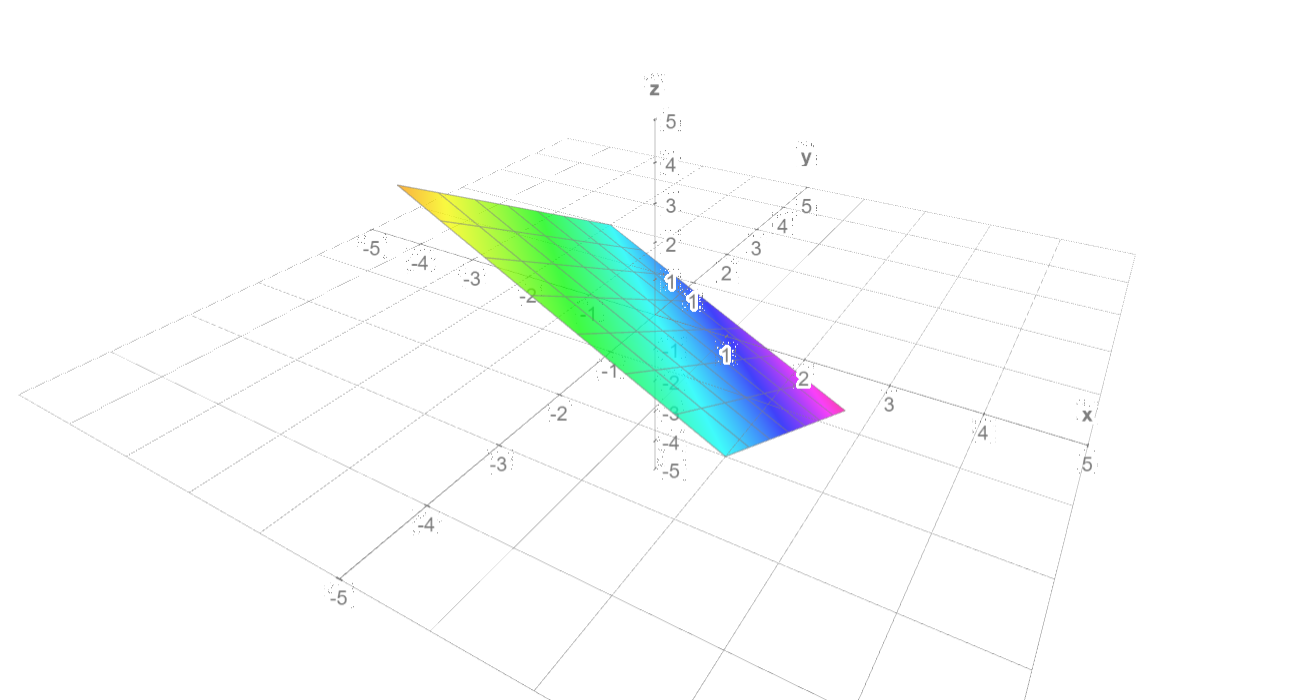
\includegraphics[width=0.8\textwidth]{_files/_images/1.png}
    \caption{Grafico della funzione $z(x_1,x_2) = -x_1-x_2$ in un dominio limitato per semplicità}
    \label{fig:mia_immagine}
\end{figure}

\newpage

\subsection{Curve di Livello}
Per iniziare a introdurre questo argomento, osserva questo, data una funzione a due variabili:
\begin{equation}
    z = f(x,y)
\end{equation}
I punti sulla superficie che si andrà a formare dalla funzione, saranno dei punti:
\begin{equation}
    \{(x,y,z) \in D : z = f(x,y)\}
\end{equation}
Ora considera l'equazione:
\begin{equation}
    f(x,y) = k
\end{equation}
Significa sostanzialmente, $f(x,y) = k = z$, cioè questa \textbf{equazione identifica i punti sulla superficie tali che}:
\begin{equation}
    \{(x,y,k) : f(x,y) = k\}
\end{equation} 
Ora c'è un altro modo per identificare questi punti sulla superficie, cioè si prende il piano di equazione:
\begin{equation}
    z = k
\end{equation}
\begin{observation}{Equazione del piano}
Nota che $z = k$ si può scrivere, come scrivo in una variabile $y = k$, scrivo anche z = k, cioè è un piano che identifica tutti i punti $(x,y,k)$ a quota k,
cioè posso vederlo come una funzione, per qualsiasi punto $(x,y)$, mi restituisce sempre k
\end{observation}
Si prendono i punti $(x,y,z)$ sulla superficie della funzione.

I punti che vengono fuori dall'intersezione del piano $z = k$ e la supeficie della funzione, identificano i punti:
\begin{equation}
    \{(x,y,k) : f(x,y) = k\}
\end{equation}
Cioè i punti che soddisfano l'equazione:
\begin{equation}
    f(x,y) = k
\end{equation}
\begin{figure}[htbp]
    \centering
    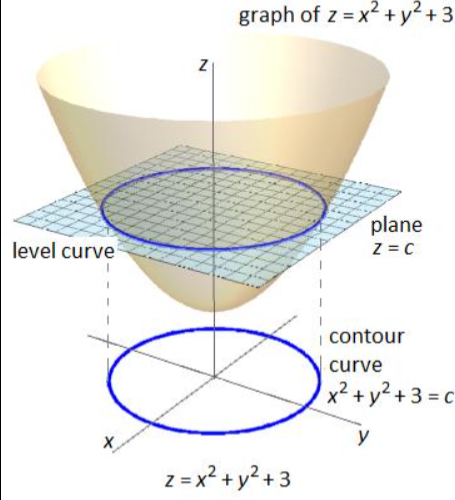
\includegraphics[width=0.4\textwidth]{_files/_images/2.png}
    \caption{Il cerchio blu a quota k, indica tutti i punti $\{(x,y,k) : f(x,y) = k\}$ }
    \label{fig:mia_immagine}
\end{figure}

Ora se dalla definizione di questi punti, elimino \textbf{la quota k}, allora usciranno tutti i punti:
\begin{equation}
    \{(x,y) : f(x,y) = k\}
\end{equation}
\textbf{Cioè è come se proietassi i punti sull'asse xy, come vedi nella figura sopra.}
Questa \textbf{è l'esatta definizione di Curva di livello}
\begin{definition}{Curva di Livello}
    \begin{equation}
        L_k = \{(x,y) \in D : f(x,y) = k \}
    \end{equation}
    Cioè l'insieme dei punti $(x,y)$ che soddisfano $f(x,y) = k$, cioè come nell'immagine di prima i punti proiettati sull'asse xy
\end{definition}
La bellezza delle curve di livello è che si possono rappresentare in un piano con assi xy, cioè dato che $k$ è costante, quello che si fa è scrivere :
\begin{equation}
    y = x - k
\end{equation}
Se f(x,y) = x + y.


Nel caso di \textbf{funzioni lineari} (cioè su quelle su cui stiamo lavorando noi), ci ritroveremo su curve di livello che sono delle rette, come in questo caso:

\begin{figure}[htbp]
    \centering
    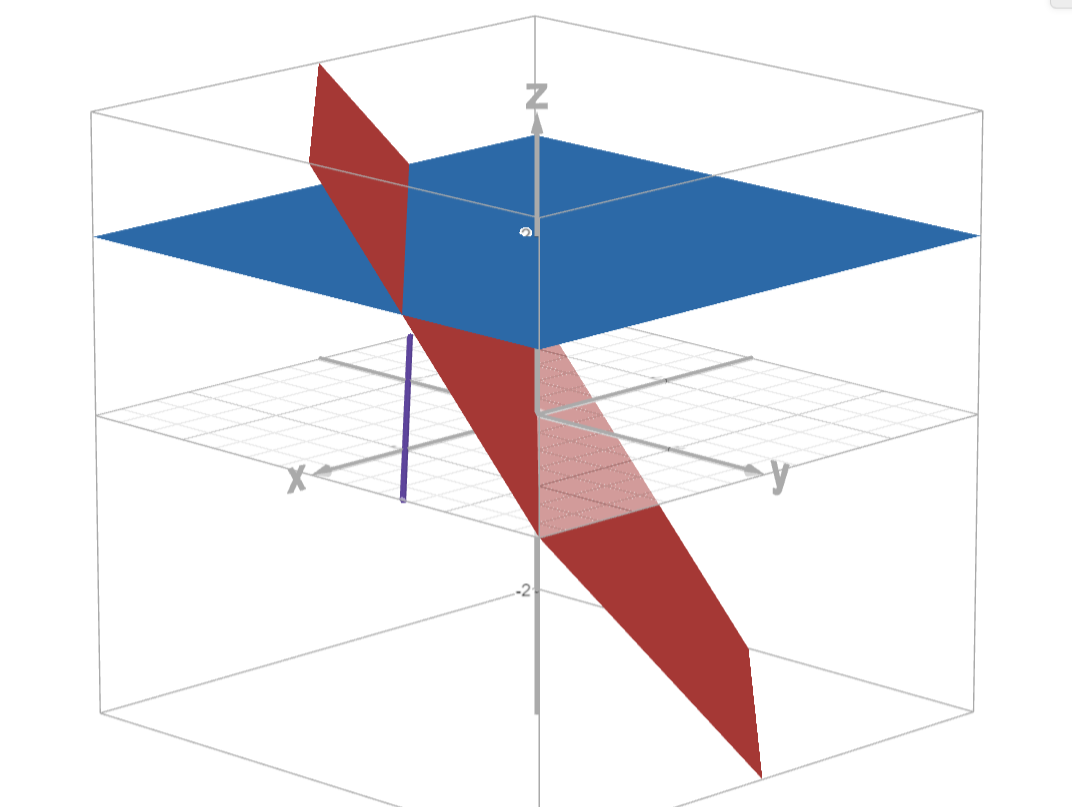
\includegraphics[width=0.4\textwidth]{_files/_images/3.png}
    \caption{In Rosso la funzione $f(x,y) = x - y$ , in blu il piano $z$ = 2 e in viola la curva di livello $L_2$ della funzione, y = x - 2}
    \label{fig:mia_immagine}
\end{figure}

In generale nelle funzioni lineari, ci troveremo a lavorare su delle rette, e variando k, ci troveremo delle rette parallele, chiamati fasci di rette.

\paragraph{Esempio di Curva di Livello}
Consideriamo la funzione:
\begin{equation}
    z(x,y) = -x-y
\end{equation}
Ora scelgo k = 3, e voglio visualizzare la curva di livello, per quel k.

Considero l'equazione:
\begin{equation}
    -x-y = 3
\end{equation}
Questa equazione considera tutti i punti sulla superficie:
\begin{equation}
    \{(x,y,3) : 3 = -x - y \}
\end{equation}

Ora per identificare la curva di livello, basta levare la quota k, e quindi:
\begin{equation}
    L_3 = \{(x,y) : 3 = -x - y \}
\end{equation}
Cioè tutti i punti $(x,y)$ sul piano che soddisfano l'equazione:
\begin{equation}
    -x-y = 3
\end{equation}
Ma questa può essere equivalentemente riscritta come:
\begin{equation}
    y = x-3
\end{equation}
\textbf{Quindi abbiamo esplicitato che è una retta nel piano, ma già lo era , noi lo abbiamo solo esplicitato.}
Noi abbiamo scelto un k a piacere, ma per funzioni lineari, al variare di k, si individua un fascio di rette parallele



Ora sapendo questo ritorniamo al nostro esempio di prima, e continuiamolo.

Per una funzione lineare a due variabili della forma

\begin{equation}
f(x_1,x_2) = ax_1 + bx_2,
\end{equation}

le \textbf{curve di livello} sono definite ponendo la funzione uguale a una costante \(d\):

\begin{equation}
ax_1 + bx_2 = d.
\end{equation}

Al variare di \(d\), si ottiene quindi un \textbf{fascio di rette parallele tra loro}. Infatti, i coefficienti \(a\) e \(b\) rimangono invariati, mentre cambia solamente il termine noto \(d\). Di conseguenza, la pendenza delle rette rimane sempre la stessa, mentre esse si spostano nel piano.

Dal punto di vista geometrico, il grafico di una funzione lineare a due variabili è un \textbf{piano nello spazio tridimensionale}. Intersecando questo piano con un piano orizzontale di equazione

$$
z=d,
$$

si ottiene una retta nello spazio. La proiezione di tale retta sul piano \(x_1x_2\) è proprio la curva di livello

$$
ax_1 + bx_2 = d.
$$

Pertanto, al variare di \(d\), si ottengono diverse curve di livello, tutte costituite da rette parallele tra loro.

\begin{figure}[htbp]
\centering
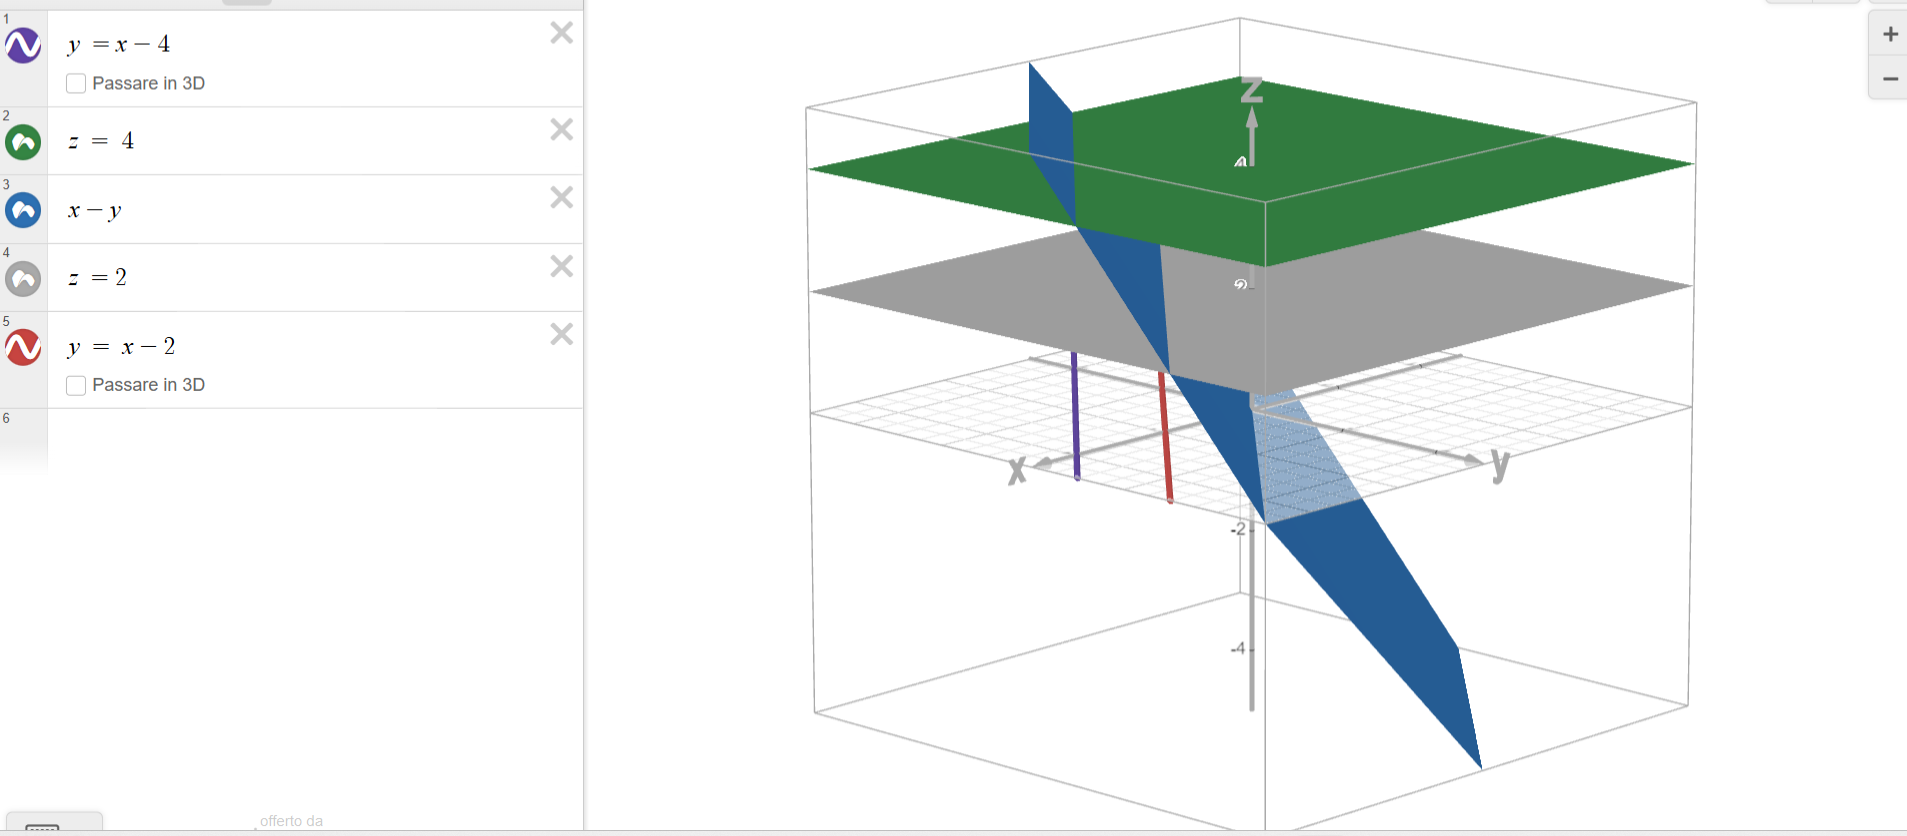
\includegraphics[width=0.8\textwidth]{_files/_images/4.png}
\caption{Due curve di livello, per \(k=2\) e \(k=4\), della funzione lineare \(f(x_1,x_2)=-x_1-x_2\).}
\label{fig:mia_immagine}
\end{figure}



\newpage
Ora visualizziamole dal lato, cosi è piu semplice lavorarci:
\begin{figure}[htbp]
\centering
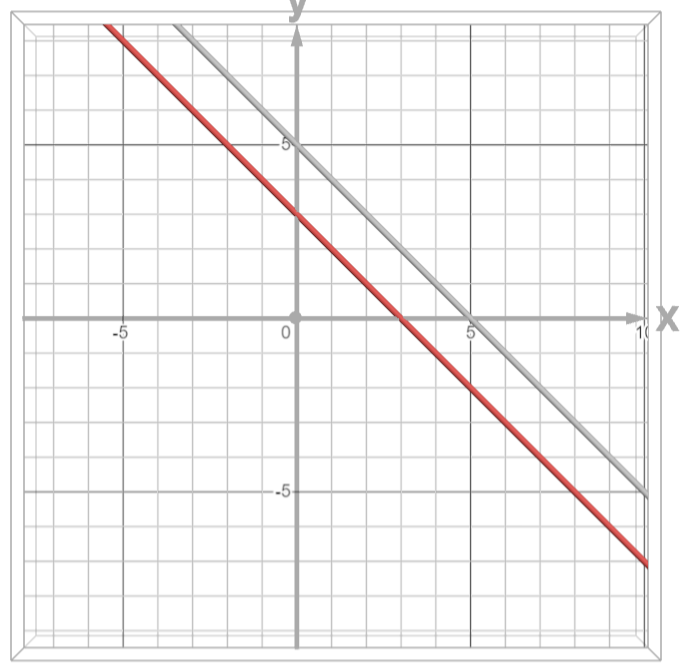
\includegraphics[width=0.4\textwidth]{_files/_images/5.png}
\caption{Due curve di livello, per \(k=3\) e \(k=5\), della funzione lineare \(f(x_1,x_2)=-x_1-x_2\).}
\label{fig:mia_immagine}
\end{figure}

Il vettore

\begin{equation}
\mathbf{n} = (a,b)
\end{equation}

è detto \textbf{vettore normale} alle rette. Esso è perpendicolare alla direzione delle rette, cioè forma con essa un angolo di \(90^\circ\).

È importante distinguere tra la \textbf{posizione} del vettore e la sua \textbf{direzione}: il vettore ((a,b)) non deve necessariamente intersecare la retta. Quando diciamo che il vettore è perpendicolare alla retta, ci riferiamo alla sua \textbf{direzione}.

Poiché tutte le rette

\[
ax_1+bx_2=d
\]

sono parallele tra loro, il vettore ((a,b)) è normale a \textbf{tutte} le rette della famiglia, indipendentemente dal valore di (d).

Inoltre, al variare di (d), le rette si spostano parallelamente a se stesse. 
\textbf{La direzione dello spostamento è proprio quella individuata dal vettore normale ((a,b)), se \(d\) aumenta, le rette si spostano nel verso di \((a,b)\); se \(d\) diminuisce, si spostano nel verso opposto.}


Ritorniamo a lavorare con il nostro esempio originale:
\begin{equation}
    f(x_1,x_2) = -x_1 - x_2
\end{equation}
Consideriamo le curve di livello al variare di d (nella figura 2.6 sotto):
\begin{equation}
    -x_1 - x_2 = d
\end{equation}
Ora nota che il vettore $(a,b) = (-1,-1)$ è normale rispetto a tutte le rette del fascio, se \(d\) aumenta, la retta si sposta nel verso di \((a,b)\); se \(d\) diminuisce, si sposta nel verso opposto.
\begin{figure}[htbp]
\centering
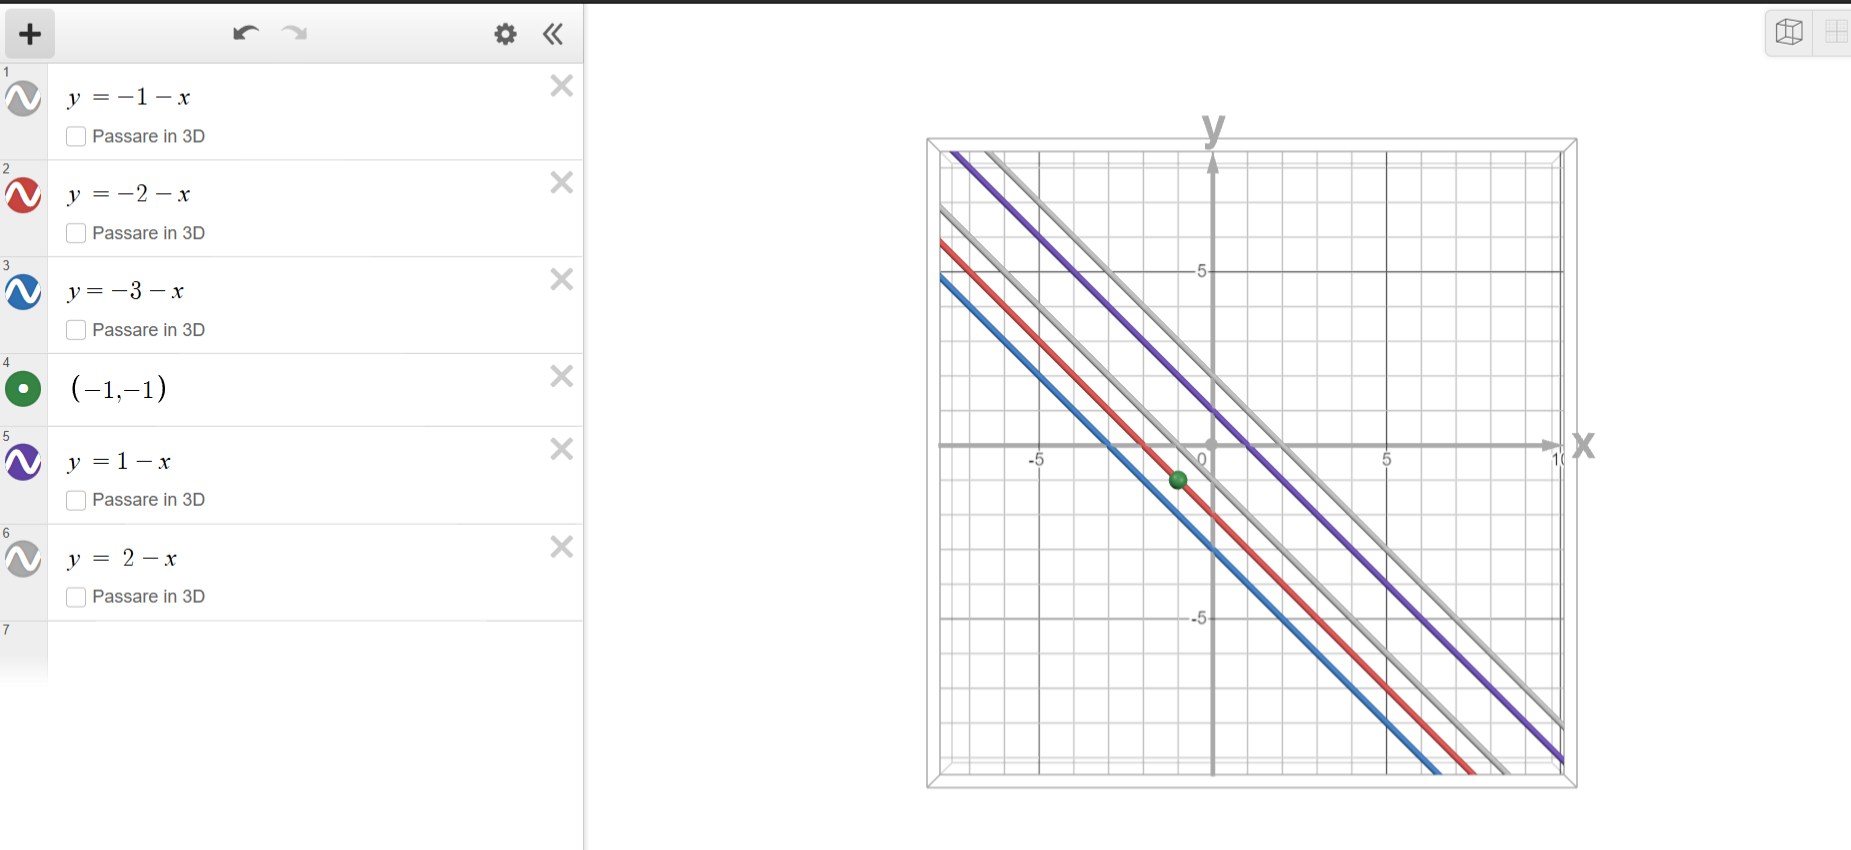
\includegraphics[width=0.6\textwidth]{_files/_images/6.png}
\caption{Curve di livello, della funzione lineare \(f(x_1,x_2)=-x_1-x_2\), e vettore $(a,b) = (-1,-1)$ che indica gli spostamenti del fascio di rette}
\label{fig:curve}
\end{figure}

\clearpage
Ora consideriamo il nostra problema iniziale:
\begin{align*}
\min \quad z(x) &= -x_1 - x_2\\
\text{s.a.} \quad x_1 + 2x_2 &\leq 3 \\
2x_1 + x_2 &\leq 3 \\
x_j &\ge 0 \quad  j = 1, 2.
\end{align*}

Ora consideriamo il primo vincolo, ragionamento analogo si fa con il secondo vincolo.
Consideriamo l'equazione:
\begin{equation}
    x_1 + 2x_2 = 3
\end{equation}
Questa viene rappresenata nel piano in questo modo:
\begin{figure}[h]
\centering
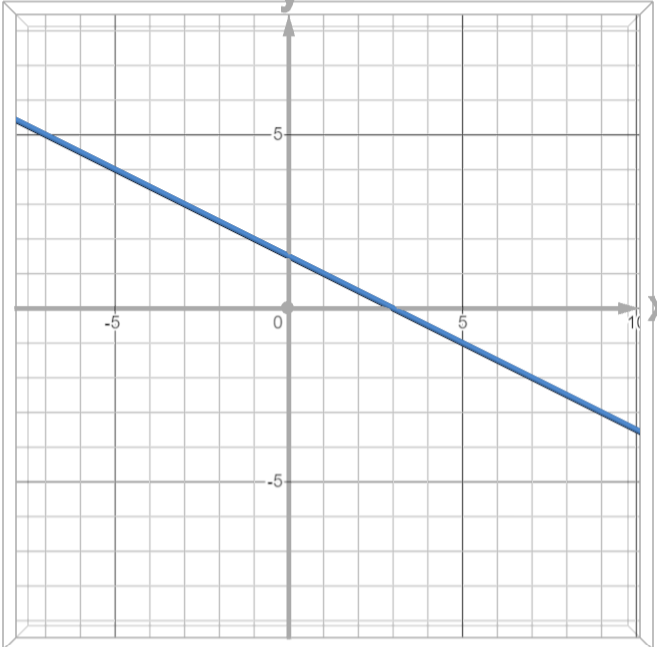
\includegraphics[width=0.3\textwidth]{_files/_images/7.png}
\label{fig:curve}
\end{figure}
\\
Tramite il vettore $(a,b) = (1,2)$ io posso dire sostanzialmente gli insiemi di punti che soddisfano
\begin{equation}
     x_1 + 2x_2 <= 3
\end{equation}
Cioè l'area:
\begin{figure}[htbp]
\centering
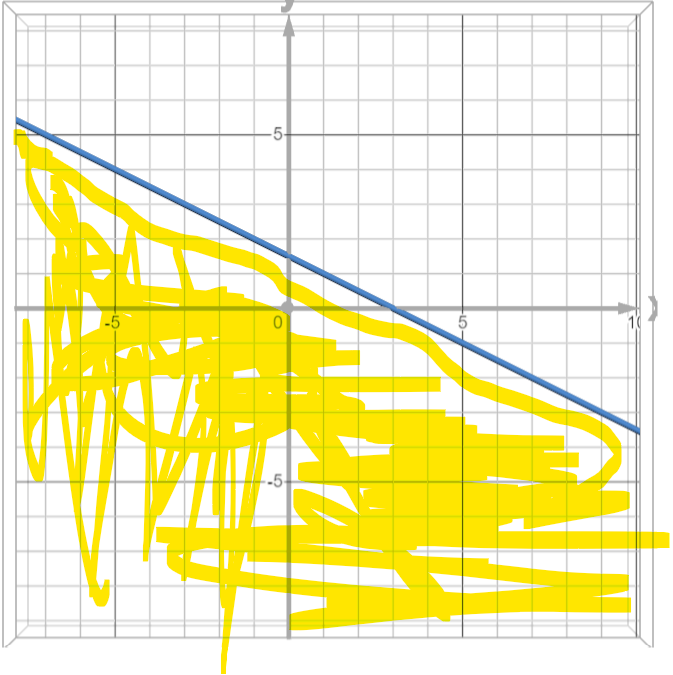
\includegraphics[width=0.3\textwidth]{_files/_images/8.png}
\label{fig:curve}
\end{figure}
Considerando anche il secondo vincolo, e considerando anche i vincoli positivi ($>=0$) sulle variabili, allora la regione ammissibile $S$, cioè
l'insieme di punti $(x,y)$ che io posso scegliere per minimizzare la funzione a due variabili $z$, è:
\begin{figure}[htbp]
\centering
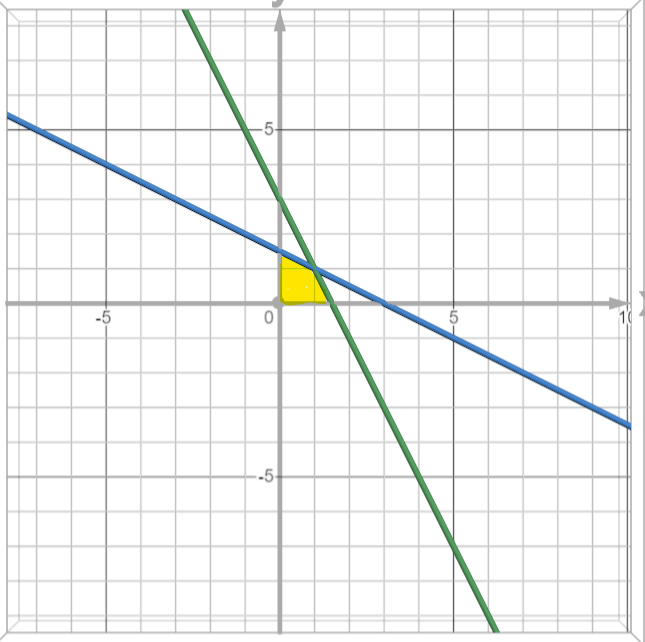
\includegraphics[width=0.2\textwidth]{_files/_images/9.png}
\label{fig:curve}
\end{figure}
Ora, data questa regione ammissibile, vogliamo capire come scegliere la coppia $(x_1,x_2)$ che rende minima la funzione obiettivo.

\clearpage

Consideriamo le curve di livello della funzione obiettivo

$$
z(x_1,x_2)=-x_1-x_2.
$$

Le curve di livello sono ottenute fissando un valore $k$ e imponendo

$$
-x_1-x_2=k.
$$

Al variare di $k$ otteniamo quindi un insieme infinito di rette parallele, ognuna delle quali rappresenta tutti i punti del piano in cui la funzione assume lo stesso valore $k$.

\begin{figure}[htbp]
\centering
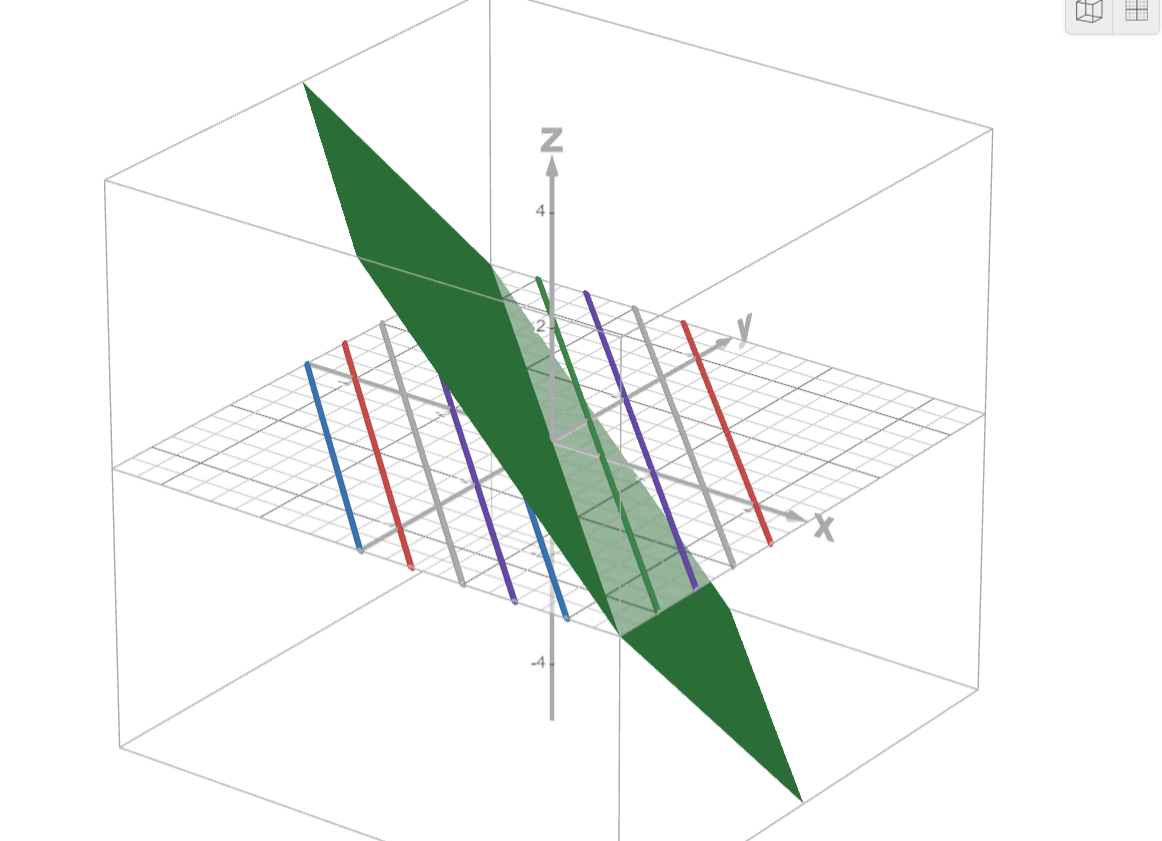
\includegraphics[width=0.4\textwidth]{_files/_images/10.png}
\label{fig:curve}
\end{figure}

Le curve di livello, considerate nel piano $(x_1,x_2)$, ci permettono quindi di visualizzare come varia il valore della funzione obiettivo.

In particolare, consideriamo il vettore

$$
(-1,-1).
$$

Questo vettore indica la direzione nella quale la funzione cresce più rapidamente. Infatti, esso coincide con il gradiente della funzione:

$$
\nabla z=(-1,-1).
$$

Muovendoci nella direzione indicata da questo vettore, passiamo da curve di livello associate a valori di $k$ sempre maggiori. Poiché su una curva di livello vale per i punti $(x,y)$ su quella curva di livello

$$
z(x_1,x_2)=k,
$$

un valore maggiore di $k$ corrisponde necessariamente a un valore maggiore della funzione obiettivo.

Ad esempio, se ci troviamo su una curva di livello $k=2$ e ci spostiamo nella direzione di $(-1,-1)$, incontreremo curve di livello associate a valori come $k=3$, $k=4$, ecc. In questa direzione, quindi, la funzione assume valori sempre maggiori.

Al contrario, muovendoci nella direzione opposta,

$$
(1,1),
$$

attraversiamo curve di livello associate a valori di $k$ sempre minori. Questa è quindi la direzione di diminuzione della funzione obiettivo.

Nel problema di ottimizzazione, però, non possiamo muoverci liberamente nel piano: dobbiamo rimanere all'interno della regione ammissibile. Per trovare il minimo, dobbiamo quindi cercare di spostarci nella direzione in cui la funzione diminuisce, cioè nella direzione $(1,1)$, finché raggiungiamo il punto più lontano possibile in tale direzione che appartiene ancora alla regione ammissibile.

Il punto, o eventualmente i punti, raggiunti sull'ultima curva di livello che interseca la regione ammissibile rappresentano le soluzioni ottime del problema.

\newpage

Rappresentando le curve di livello quindi della nostra funzione e tenendo conto dell'insieme $S$ in giallo:
\begin{figure}[htbp]
\centering
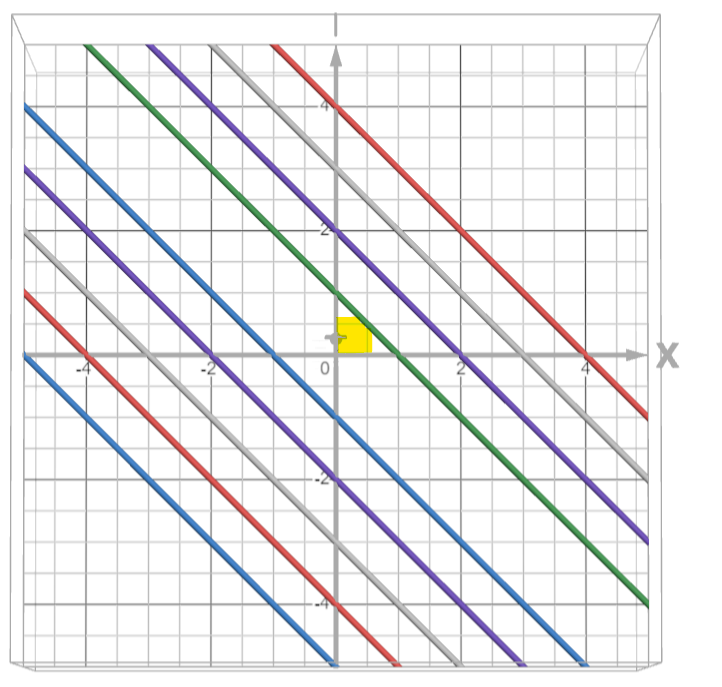
\includegraphics[width=0.4\textwidth]{_files/_images/11.png}
\label{fig:curve}
\end{figure}

O meglio si può vedere dal disegno della prof, \textbf{dove le curve di livello della funzione sono quelle trattegiate, e devi guardare solo quelle}:
\begin{figure}[htbp]
\centering
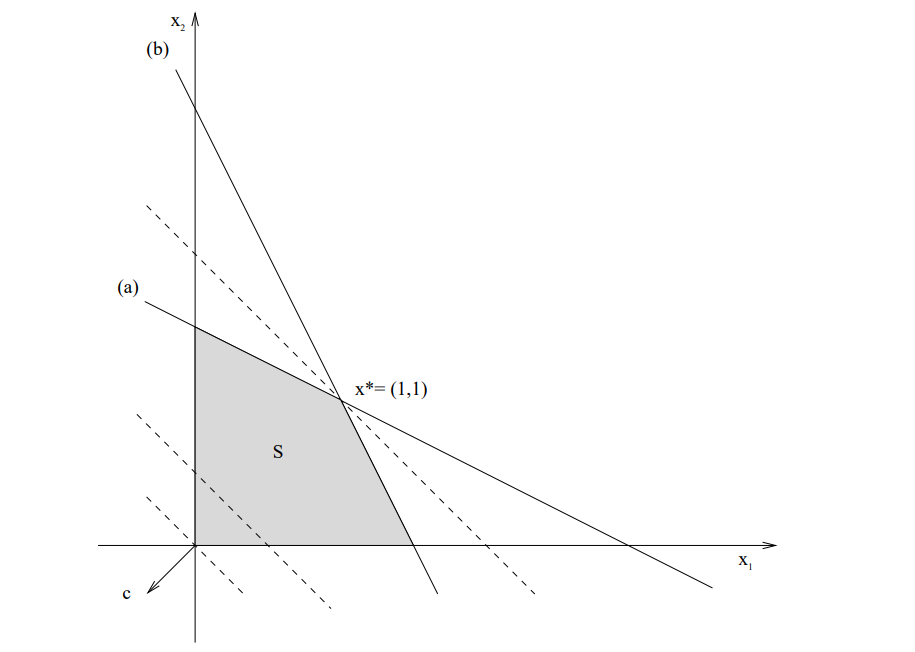
\includegraphics[width=0.4\textwidth]{_files/_images/12.png}
\label{fig:curve}
\end{figure}

Consideriamo quindi quella curva di livello con valore $k=-2$, che rappresenta il minimo valore che la funzione può assumere nell'insieme ammissibile $S$. Non possiamo infatti spostarci ulteriormente nella direzione di diminuzione della funzione, perché usciremmo dalla regione ammissibile.

In generale, se la regione ammissibile contenesse un tratto della curva di livello $k=-2$, potremmo scegliere uno qualsiasi degli infiniti punti appartenenti a quel tratto,\textbf{poiché tutti questi punti avrebbero lo stesso valore della funzione obiettivo}. In questo caso, però, la regione ammissibile non contiene altri punti della curva di livello $k=-2$: di conseguenza, il punto di contatto con la regione ammissibile costituisce l'unica soluzione ottima.

La regione ammissibile S del problema dell'esempio precedente è limitata e la soluzione ottima è unica. Attraverso il seguente esempio vengono
descritti altri casi possibili.


\section{Esempio: diversi casi possibili} Consideriamo la regione ammissibile $S$ descritta dai vincoli: \[ -x_1+x_2\leq 1 \] e \[ x_j\geq 0,\qquad j=1,2. \] Quindi: \[ S= \left\{ (x_1,x_2)\in\mathbb{R}^2: -x_1+x_2\leq1,\; x_1\geq0,\; x_2\geq0 \right\}. \] 
\begin{figure}[htbp]
\centering
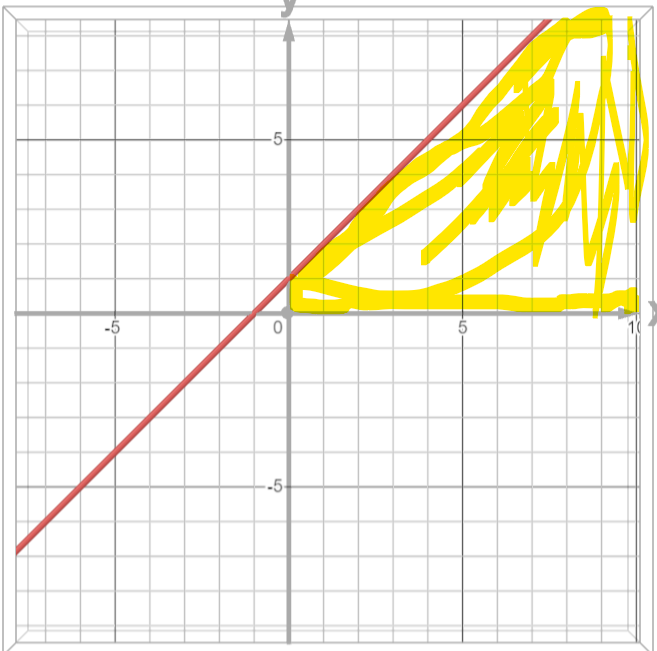
\includegraphics[width=0.4\textwidth]{_files/_images/13.png}
\label{fig:curve}
\end{figure}


Supponiamo di voler minimizzare diverse funzione obiettivo lineari.

A seconda del vettore dei costi $c$ si possono presentare diversi casi.
\begin{center}
    Tieni conto che una volta definito c, si è definito la funzione lineare, non c'è altro piu da definire,
    quindi $c = (1,1)$, identifica una sola funzione lineare, cioè $z(x_1,x_2) = x_1 + x_2$.
\end{center}
\subsection{Caso 1: soluzione ottima unica} Sia: \[ c=(1,1). \] La funzione obiettivo è: \[ z(x)=x_1+x_2. \] Poiché $x_1,x_2\geq0$, il valore minimo possibile è $0$, ottenuto per: \[ x^*=(0,0). \] Quindi: \[ \boxed{x^*=(0,0)} \] è l'unica soluzione ottima. Il valore ottimo è: \[ z(x^*)=0. \] Questo è un caso in cui esiste una \textbf{unica soluzione ottima}. 
\subsection{Caso 2: infinite soluzioni ottime e insieme delle soluzioni ottime limitato} Sia: \[ c=(1,0). \] La funzione obiettivo diventa: \[ z(x)=x_1. \] 
\begin{figure}[h]
\centering
\begin{tikzpicture}
\begin{axis}[
    axis lines=middle,
    xlabel={$x_1$},
    ylabel={$x_2$},
    xmin=-1, xmax=5,
    ymin=-1, ymax=4,
    grid=both,
    axis equal
]

% Curve di livello
\addplot[domain=-1:4] coordinates {(1,-1) (1,4)};
\addplot[domain=-1:4] coordinates {(2,-1) (2,4)};
\addplot[domain=-1:4] coordinates {(3,-1) (3,4)};

% Vettore dei costi
\addplot[
    -{Latex[length=3mm]},
    very thick
] coordinates {(0,0) (2,0)};

\node at (axis cs:2.4,0.3) {$c=(1,0)$};

\end{axis}
\end{tikzpicture}
\caption{Curve di livello e vettore dei costi $c=(1,0)$.}
\end{figure}

Poiché $x_1\geq0$, il valore minimo è ottenuto imponendo: \[ x_1=0. \] I punti ammissibili con $x_1=0$ devono inoltre soddisfare: \[ x_2\leq1, \qquad x_2\geq0. \] Pertanto ogni punto della forma \[ \boxed{ x^*=(0,x_2),\qquad 0\leq x_2\leq1 } \] è una soluzione ottima. Il valore ottimo è: \[ z(x^*)=0. \] In questo caso esistono \textbf{infiniti punti ottimi}, ma l'insieme delle soluzioni ottime è \textbf{limitato}. Infatti: \[ \{(0,x_2):0\leq x_2\leq1\} \] è un segmento limitato. 
\subsection{Caso 3: infinite soluzioni ottime e insieme delle soluzioni ottime illimitato} Sia: \[ c=(0,1). \]
\begin{figure}[h]
\centering
\begin{tikzpicture}
\begin{axis}[
    axis lines=middle,
    xlabel={$x_1$},
    ylabel={$x_2$},
    xmin=-1, xmax=5,
    ymin=-1, ymax=5,
    grid=both,
    axis equal
]

% Curve di livello
\addplot coordinates {(-1,1) (5,1)};
\addplot coordinates {(-1,2) (5,2)};
\addplot coordinates {(-1,3) (5,3)};

% Vettore dei costi
\addplot[
    -{Latex[length=3mm]},
    very thick
] coordinates {(0,0) (0,2)};

\node at (axis cs:0.8,2.2) {$c=(0,1)$};

\end{axis}
\end{tikzpicture}
\caption{Curve di livello e vettore dei costi $c=(0,1)$.}
\end{figure}


La funzione obiettivo è: \[ z(x)=x_2. \] Poiché: \[ x_2\geq0, \] il valore minimo si ottiene ponendo: \[ x_2=0. \] Tutti i punti della forma \[ \boxed{ x^*=(x_1,0),\qquad x_1\geq0 } \] sono ammissibili e hanno: \[ z(x^*)=0. \] Quindi tutti questi punti sono soluzioni ottime. In questo caso l'insieme delle soluzioni ottime è: \[ \{(x_1,0):x_1\geq0\}, \] che è \textbf{illimitato}. È importante osservare che il fatto che l'insieme ammissibile $S$ sia infinito o illimitato non implica necessariamente che il problema sia illimitato. In questo caso, infatti, il valore ottimo esiste ed è: \[ \boxed{z^*=0}. \] 
\subsection{Caso 4: problema illimitato inferiormente} Sia: \[ c=(-1,-1). \] 
\begin{figure}[h]
\centering
\begin{tikzpicture}
\begin{axis}[
    axis lines=middle,
    xlabel={$x_1$},
    ylabel={$x_2$},
    xmin=-1, xmax=5,
    ymin=-1, ymax=5,
    grid=both,
    axis equal
]

% Curve di livello
\addplot[domain=-1:5, samples=2] {-x+1};
\addplot[domain=-1:5, samples=2] {-x+3};
\addplot[domain=-1:5, samples=2] {-x+5};

% Vettore dei costi
\addplot[
    -{Latex[length=3mm]},
    very thick
] coordinates {(0,0) (-2,-2)};

\node at (axis cs:-1.8,-1.5) {$c=(-1,-1)$};

\end{axis}
\end{tikzpicture}
\caption{Curve di livello e vettore dei costi $c=(-1,-1)$.}
\end{figure}

La funzione obiettivo è: \[ z(x)=-x_1-x_2. \], e i vincoli sono che $x_1 >= 0$ e $x_2$ >= 0, quindi ci troviamo nel quadrante a destra


Vogliamo quindi risolvere: \[ \min_{x\in S}(-x_1-x_2). \] Consideriamo la successione di punti: \[ x^{(k)}=(k,0), \qquad k=1,2,3,\ldots \] Verifichiamo che questi punti siano ammissibili. Abbiamo: \[ x_1=k\geq0, \qquad x_2=0\geq0, \] e inoltre: \[ -x_1+x_2=-k\leq1. \] Pertanto: \[ x^{(k)}\in S \qquad\forall k\geq1. \] Calcoliamo ora il valore della funzione obiettivo: \[ z(x^{(k)}) = -k-0 = -k. \] Quindi: \[ \boxed{ z(x^{(k)})=-k\longrightarrow-\infty } \] Questo significa che possiamo trovare punti ammissibili il cui costo diventa arbitrariamente piccolo. Per esempio: \[ -1,\;-10,\;-100,\;-1000,\ldots \] non esiste quindi un valore minimo finito. Si dice che il problema è \textbf{illimitato inferiormente} e si scrive: \[ \boxed{ \inf_{x\in S}z(x)=-\infty. } \]




\section{Geometria della Programmazione Lineare}
\subsection{Poliedro ed insiemi convessi}
All'inizio del corso, abbiamo fatto un esempio di un regione ammissibile $S$, lo riporto:
\begin{center}
        $$
        S = \left\{ (x,y) \in \mathbb{R}^2 : 
        \begin{array}{l}
        4x + 2y \le 40 \\
        2x + y \le 16 \\
        x \ge 0, y \ge 0
        \end{array} 
        \right\}
        $$
\end{center}
Questa regione delimita un insieme di punti sul piano:
\begin{figure}[htbp]
    \centering
    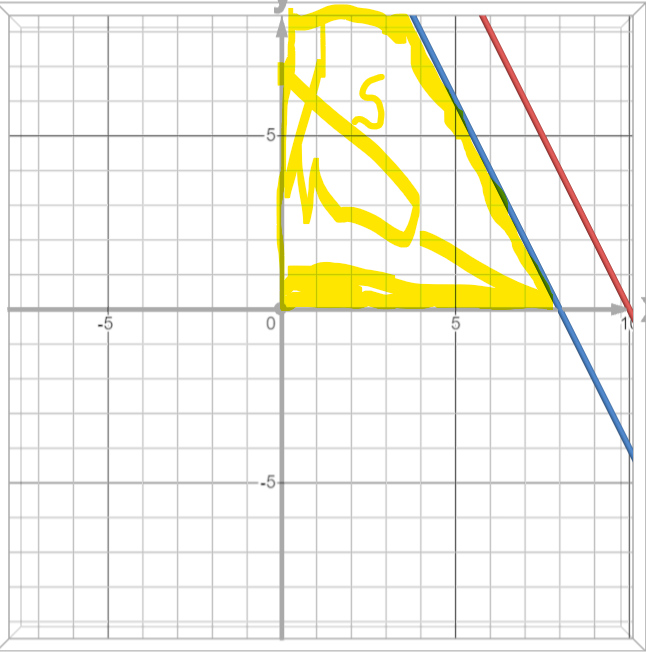
\includegraphics[width=0.4\textwidth]{_files/_images/14.png}
    \caption{L'area gialla è l'insieme dei punti della regione ammissibile S}
    \label{fig:mia_immagine}
\end{figure}
Come vedi i vincoli del problema nell'insieme $S$,sono un sistema, il che si può equivalentemente scrivere sottoforma matriciale,\textbf{come
abbiamo visto nel paragrafo apposito quando si trasformava il problema sottoforma matriciale}
Quindi si può definire:
\begin{definition}{Poliedro}
    L'insieme $P$ = \{$x \in \mathbb{R} ^ n$ | $Ax >= b$\}, dove $A \in R^{m x n}$ e $b \in \mathbb{R}^m$ è detto \textbf{poliedro}
\end{definition}
\begin{warning}
    Si scrive $>=$ nella definizione, perchè anche se abbiamo $<=$ si possono riportare alla forma di maggiore uguale.
\end{warning}
Un poliedro quindi è una regione di punti.
\begin{definition}{Insieme Limitato}
Un insieme $S \subset \mathbb{R}^n$ è detto \textbf{limitato} se esiste una costante $k$ tale che il valore assoluto di ogni componente di ogni elemento di $S$ sia minore o uguale a $k$, cioè:
\[
|x_i| \leq k,
\qquad
\forall i = 1,2,\ldots,n,
\quad
\forall x \in S.
\]
\end{definition}


Prima di passare alla prossima definizione, ricordiamo che:
\begin{equation}
    a_1 x_1 + a_2 x_2 = b
\end{equation}
Può essere vista come una curva di livello $L_b$ per la funzione, o come una funzione ad una variabile, \textbf{isolando $x_2$}.
Per ora per semplicità pensala a come una funzione ad una variabile.


\paragraph{Esempio}
Considera 
\begin{equation}
    x_1 + x_2 = 5
\end{equation}
Che isolando $x_2$ diventa:
\begin{equation}
    x_2 = 5 - x_1
\end{equation}
Questa è una retta, e descrive tutti i punti \{$(x_1,x_2)$ | $x_1 + x_2 = 5$ \}

\begin{definition}{Iperpiano}
Sia $a \in \mathbb{R}^n$ e sia $b \in \mathbb{R}$ uno scalare.
L'insieme

$$
\{x \in \mathbb{R}^n \mid a^Tx = b\}
$$

è detto \textbf{iperpiano}.
\end{definition}

\textbf{Esempio.}
Consideriamo l'iperpiano in $\mathbb{R}^2$:
\[
x_1+x_2=5.
\]

Possiamo riscriverlo come
\[
x_2=5-x_1,
\]
ottenendo quindi una retta nel piano $(x_1,x_2)$.

\begin{center}
\begin{tikzpicture}
\begin{axis}[
    axis lines=middle,
    xlabel={$x_1$},
    ylabel={$x_2$},
    xmin=-2, xmax=7,
    ymin=-2, ymax=7,
    grid=both,
    width=9cm,
    height=7cm,
    samples=100,
]
\addplot[domain=-2:7] {5-x};
\end{axis}
\end{tikzpicture}
\end{center}

La retta rappresenta tutti i punti $(x_1,x_2)\in\mathbb{R}^2$
che soddisfano l'equazione $x_1+x_2=5$.


\begin{definition}{Semi-spazio}

Sia $a \in \mathbb{R}^n$ e sia $b \in \mathbb{R}$ uno scalare.

L'insieme

$$
\{x \in \mathbb{R}^n \mid a^Tx \geq b\}
$$

è detto \textbf{semi-spazio}.

\end{definition}

In pratica, il semi-spazio è l'insieme di tutti i punti che si trovano \textbf{da un lato dell'iperpiano}

$$
a^Tx=b,
$$

in particolare dal lato individuato dalla \textbf{direzione del vettore normale} $a$.

Infatti, il vettore $a$ è perpendicolare all'iperpiano $a^Tx=b$ e indica la direzione verso cui aumenta il valore di $a^Tx$.

Il vincolo

$$
a^Tx\geq b
$$

seleziona quindi l'iperpiano stesso (perchè >=) e tutti i punti che si trovano dal lato verso cui punta il vettore $a$.

Si noti quindi che $a$ è perpendicolare all'iperpiano stesso.

Questo perchè considerando l'iperpiano

$$
H=\{x\in\mathbb{R}^n\mid a^Tx=b\}.
$$

Siano $x,y\in H$ due punti appartenenti allo stesso iperpiano. Per definizione di iperpiano, entrambi devono soddisfare l'equazione:

$$
a^Tx=b
$$

e

$$
a^Ty=b.
$$

Pertanto:

$$
a^Tx=a^Ty.
$$

Portando tutto a sinistra:

$$
a^Tx-a^Ty=0.
$$

Per la linearità del prodotto scalare:

$$
a^T(x-y)=0.
$$

Poiché il prodotto scalare tra due vettori è nullo se e solo se essi sono ortogonali, otteniamo:

$$
a\perp(x-y).
$$

\textbf{($x-y$ è il vettore che va dal punto $x$ al punto $y$)}

Quindi il vettore $a$ è ortogonale al vettore che collega due qualsiasi punti $x$ e $y$ dell'iperpiano.

In altre parole, $a$ è un \textbf{vettore normale all'iperpiano}:

$$
\boxed{a\text{ è ortogonale a ogni direzione contenuta nell'iperpiano, cioè è ortogonale a ogni vettore giacente sul piano.}}
$$

\subsection{Insiemi convessi}

\begin{definition}{Insieme convesso}

Un insieme $S\subset\mathbb{R}^n$ è detto \textbf{convesso} se

$$
\forall x,y\in S,\quad \forall\lambda\in[0,1],
$$

risulta

$$
v = \lambda x+(1-\lambda)y\in S.
$$

\end{definition}

In altre parole, un insieme è convesso se, presi \textbf{due qualsiasi punti} $x,y\in S$, tutti i punti del segmento che li collega appartengono ancora a $S$.


$v$ \textbf{rappresenta un punto fra il segmento che collega $y$ e $x$ e adesso vedremo perchè:}


Possiamo riscrivere

$$
v=\lambda x+(1-\lambda)y
$$

come

$$
v=y+\lambda(x-y).
$$

In questa forma possiamo interpretare i diversi elementi come segue:

$$
\boxed{
\underbrace{y}_{\text{punto di partenza}}
+
\underbrace{\lambda}_{\text{fattore di scala}}
\underbrace{(x-y)}_{\text{vettore direzione}}
=
\underbrace{v}_{\text{punto raggiunto}}
}
$$

In particolare:
\begin{itemize}
\item $y$ rappresenta il \textbf{punto di partenza};
\item $x-y$ rappresenta la \textbf{direzione} e il magnitudo per spostarmi, da $y$ a $x$;
\item $\lambda$ rappresenta l'\textbf{ampiezza dello spostamento} lungo tale direzione (se voglio raggiungere $x$, faccio tutto lo spostamento quindi $\lambda$ = 1,
altrimenti se voglio rimanere in $y$, scelgo $\lambda$ = 0);
\item $v$ rappresenta il \textbf{punto raggiunto}.
\end{itemize}

Poiché $\lambda\in[0,1]$, il punto $v$ rimane sul segmento che collega $y$ a $x$.

\paragraph{Esempio}
Consideriamo due punti $x = (1,1)$ e $y = (2,4)$, consideriamo $x-y$, questo è il puntino grigio nello sfondo, cioè $(-1,-3)$,
\begin{figure}[htbp]
    \centering
    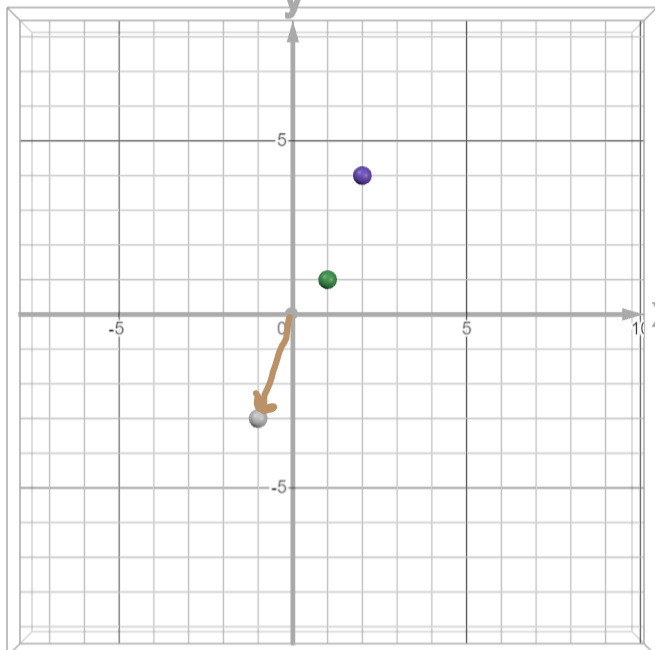
\includegraphics[width=0.2\textwidth]{_files/_images/15.png}
    \caption{$x = (1,1)$ e $y = (2,4)$, sono rispettivamente il verde e il viola, e il vettore marrone che raggiunge il punto grigio,
    indica il vettore differenza,con direzione e magnitudo per spostarsi da $y$ a $x$}
    \label{fig:mia_immagine}
\end{figure}

Se vedi quel vettore indica la direzione e il magnitudo per spostarmi da $y$ a $x$, \textbf{per spostarmi però non mi basta solo questo vettore, ma devo prendere un punto di inizio, in questo caso prendo $y = (1,1)$ (dato che mi voglio spostare da $y$ a $x$)}
Tramite solo questi due elementi, io riuscirei a spostarmi da $y$ a $x$, in modo completo. \textbf{Ma dato che voglio rappresentare tutti i punti sul segmento da $y$ a $x$, quello
che faccio è aggiungere un fattore di scala}, chiamato $\lambda$,questo mi permette di inviduare tutti i punti su quel segmento, in particolare:
\begin{itemize}
    \item $\lambda$ = 0, indica che resto fermo sul punto $y$.
    \item $\lambda$ = 1, sfrutto tutto il vettore e identifico il punto $x$.
\end{itemize} 
\begin{center}
    In un insieme convesso, tutti i punti su quel segmento, quindi $\forall \lambda \in [0,1]$ devono appartenere a $S$.
\end{center}
Questo poi \textbf{deve valere} per ogni segmento che prendo fra due punti arbitrari in $S$

\begin{definition}{Combinazione convessa}

Siano $x_1,x_2,\ldots,x_k$ vettori di $\mathbb{R}^n$ e siano
$\lambda_1,\lambda_2,\ldots,\lambda_k$ scalari non negativi tali che la loro somma sia uguale a $1$, cioè

$$
\lambda_i\geq0,\qquad i=1,2,\ldots,k
$$

e

$$
\sum_{i=1}^{k}\lambda_i=1.
$$

Il vettore

$$
\sum_{i=1}^{k}\lambda_i x_i
$$

è detto \textbf{combinazione convessa} dei vettori
$x_1,x_2,\ldots,x_k$.

La combinazione convessa permette di ottenere un \textbf{nuovo vettore} a partire dai vettori $x_1,\ldots,x_k$, utilizzando i coefficienti $\lambda_i$ come dei ``pesi''.

Poiché:

$$
\lambda_i\geq0
\qquad\text{e}\qquad
\sum_{i=1}^{k}\lambda_i=1,
$$

il vettore risultante rimane sempre nella regione geometrica ``compresa'' dai vettori di partenza, considerando questi ultimi come punti dello spazio.

\paragraph{Caso di due vettori.}

Consideriamo due vettori $x_1$ e $x_2$:

$$
x=\lambda_1x_1+\lambda_2x_2
$$

con

$$
\lambda_1,\lambda_2\geq0,
\qquad
\lambda_1+\lambda_2=1.
$$

Possiamo porre $\lambda_2=\lambda$, ottenendo:

$$
x=(1-\lambda)x_1+\lambda x_2,
\qquad
0\leq\lambda\leq1.
$$

Il vettore risultante $x$ appartiene quindi al \textbf{segmento che unisce $x_1$ e $x_2$}.

\begin{center}
\begin{tikzpicture}[scale=1.1]

\draw[->] (-0.5,0) -- (6,0) node[right] {$x_1$};

\fill (1,0) circle (2pt) node[below] {$x_1$};
\fill (4,0) circle (2pt) node[below] {$x$};
\fill (5.5,0) circle (2pt) node[below] {$x_2$};

\draw[very thick] (1,0) -- (5.5,0);

\end{tikzpicture}
\end{center}

Variando $\lambda$ tra $0$ e $1$, il punto $x$ può assumere \textbf{tutte le posizioni del segmento}.

In particolare:

$$
\lambda=0 \Rightarrow x=x_1
$$

e

$$
\lambda=1 \Rightarrow x=x_2.
$$


\end{definition}



\begin{definition}{Combinazione Convessa - Continuo}
\paragraph{Caso di tre vettori.}

Consideriamo ora tre vettori $x_1,x_2,x_3$:

$$
x=\lambda_1x_1+\lambda_2x_2+\lambda_3x_3
$$

con

$$
\lambda_1,\lambda_2,\lambda_3\geq0,
\qquad
\lambda_1+\lambda_2+\lambda_3=1.
$$

Se i tre punti $x_1,x_2,x_3$ \textbf{non sono allineati}, il punto $x$ appartiene al \textbf{triangolo} avente come vertici $x_1,x_2,x_3$.

\begin{center}
\begin{tikzpicture}[scale=1.1]

\coordinate (A) at (0,0);
\coordinate (B) at (5,0);
\coordinate (C) at (2,3);

\draw[thick] (A) -- (B) -- (C) -- cycle;

\fill (A) circle (2pt) node[below left] {$x_1$};
\fill (B) circle (2pt) node[below right] {$x_2$};
\fill (C) circle (2pt) node[above] {$x_3$};

\fill (2.4,1.2) circle (2pt) node[right] {$x$};

\end{tikzpicture}
\end{center}

La posizione del punto $x$ all'interno del triangolo dipende dai valori dei coefficienti $\lambda_1,\lambda_2,\lambda_3$.

Ad esempio:

$$
x=0.2x_1+0.3x_2+0.5x_3
$$

individua uno specifico punto all'interno del triangolo.

Se uno dei coefficienti è uguale a $0$, il punto può trovarsi sul bordo del triangolo. Ad esempio:

$$
x=0.5x_1+0.5x_2+0x_3
$$

produce un punto appartenente al segmento che collega $x_1$ e $x_2$.

Se invece un coefficiente è uguale a $1$, tutti gli altri devono essere uguali a $0$ e si ottiene direttamente uno dei vettori di partenza. Ad esempio:

$$
x=1x_1+0x_2+0x_3=x_1.
$$

\paragraph{In generale.}

Il ragionamento può essere esteso a un numero qualsiasi di vettori. La combinazione convessa

$$
x=\sum_{i=1}^{k}\lambda_i x_i
$$

produce un punto appartenente alla regione convessa generata dai punti $x_1,\ldots,x_k$.

La forma geometrica di questa regione dipende dal numero di punti, dalla dimensione dello spazio e dalla loro disposizione.

Ad esempio, in $\mathbb{R}^2$, quattro punti possono generare un quadrilatero:

\begin{center}
\begin{tikzpicture}[scale=1.0]

\coordinate (A) at (0,0);
\coordinate (B) at (4,0);
\coordinate (C) at (5,2.5);
\coordinate (D) at (1,3);

\draw[thick] (A) -- (B) -- (C) -- (D) -- cycle;

\fill (A) circle (2pt) node[below left] {$x_1$};
\fill (B) circle (2pt) node[below right] {$x_2$};
\fill (C) circle (2pt) node[above right] {$x_3$};
\fill (D) circle (2pt) node[above left] {$x_4$};

\end{tikzpicture}
\end{center}


\end{definition}



\newpage

\begin{definition}{Inviluppo convesso}

Si dice \textbf{inviluppo convesso} dei vettori
$x_1,x_2,\ldots,x_k$ l'insieme di tutti i vettori che possono essere ottenuti come combinazione convessa di
$x_1,x_2,\ldots,x_k$ e si indica con

$$
\operatorname{conv}(x_1,x_2,\ldots,x_k).
$$

Pertanto:

$$
\boxed{
\operatorname{conv}(x_1,\ldots,x_k)
=
\left\{
\sum_{i=1}^{k}\lambda_i x_i
\;\middle|\;
\lambda_i\geq0,\;
\sum_{i=1}^{k}\lambda_i=1
\right\}.
}
$$

In altre parole, l'inviluppo convesso è l'\textbf{insieme di tutti i punti che possiamo ottenere facendo variare i coefficienti $\lambda_i$}, rispettando sempre le condizioni:

$$
\lambda_i\geq0
\qquad\text{e}\qquad
\sum_{i=1}^{k}\lambda_i=1.
$$

Possiamo quindi interpretarlo geometricamente come la \textbf{regione convessa più piccola che contiene tutti i punti $x_1,\ldots,x_k$}, quindi nel caso di due vettori,
\textbf{l'inviluppo convesso coincide con il segmento chiuso e convesso $[x_1,x_2]$}. Se aggiungessi un terzo punto non allineato l'inviluppo convesso diventerebbe l'intera area del triangolo con vertici $x_1, x_2, x_3$.

\begin{itemize}

\item \textbf{2 vettori:} l'inviluppo convesso è il \textbf{segmento} che li collega.

\item \textbf{3 vettori non allineati:} l'inviluppo convesso è il \textbf{triangolo}, compreso il suo interno e il suo bordo.

\item \textbf{Più vettori:} l'inviluppo convesso è la regione convessa che contiene tutti i punti dati. In $\mathbb{R}^2$ può essere, ad esempio, un triangolo, un quadrilatero, un pentagono, ecc.

\end{itemize}

\textbf{Idea fondamentale:}

$$
\boxed{
\text{vario i }\lambda_i
\quad\Longrightarrow\quad
\text{vario il punto }x
\quad\Longrightarrow\quad
\text{ottengo tutto l'inviluppo convesso}
}
$$

Quindi la \textbf{combinazione convessa} produce \textbf{un singolo punto} (per una specifica scelta dei $\lambda_i$), mentre l'\textbf{inviluppo convesso} contiene \textbf{tutti i punti ottenibili} facendo variare i $\lambda_i$ nel rispetto delle condizioni richieste.

\end{definition}


\begin{theorem}{Proprietà degli insiemi convessi}

Valgono le seguenti proprietà, di cui trascuriamo in questo contesto la verifica.

\begin{enumerate}[label=(\alph*)]

    \item L'intersezione di insiemi convessi è un insieme convesso.

    \item Ogni poliedro è un insieme convesso.

    \item Il vettore che esce fuori dalla combinazione convessa di un numero finito di elementi di un insieme convesso $S$ appartiene all'insieme convesso $S$.

    \item L'inviluppo convesso di un numero finito di vettori è un insieme convesso.

\end{enumerate}

\end{theorem}

\newpage

\subsection{Punti estremi, vertici e soluzioni di base ammissibili}
In questo paragrafo daremo tre definizioni equivalenti di vertice.

\begin{definition}{Punto estremo}
Sia $P = \{x \in \mathbb{R}^n \mid A x \ge b\}$ (oppure $A x \le b$) un poliedro espresso da un sistema di disuguaglianze lineari. 
Un vettore $x \in P$ è detto \emph{punto estremo} di $P$ se non esistono due vettori $y, z \in P$ ($y, z \neq x$) ed uno scalare $\lambda \in [0, 1]$, tali che $x = \lambda y + (1 - \lambda)z$.
\end{definition}


\begin{figure}[htbp]
    \centering
    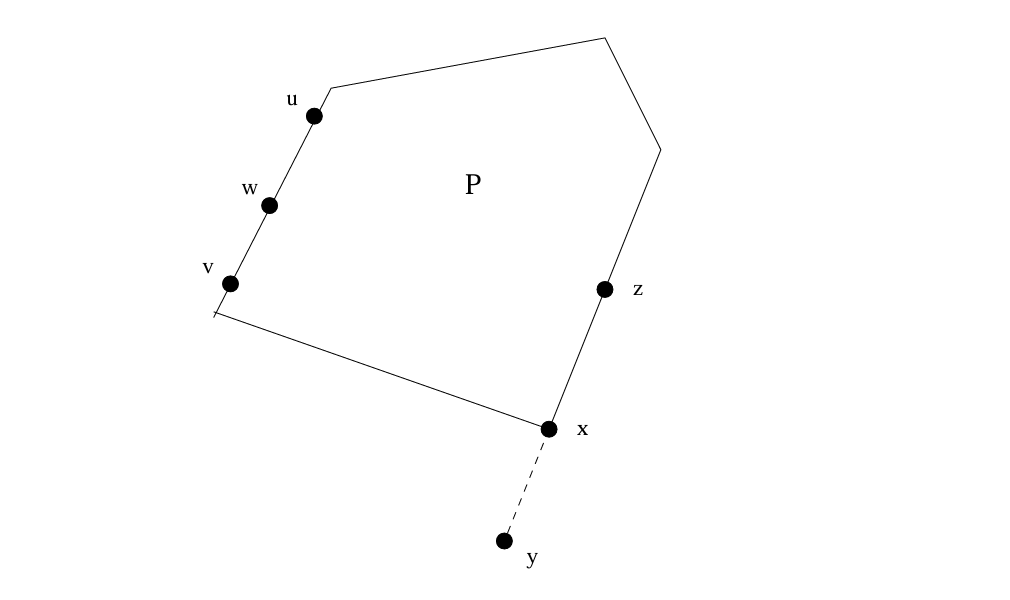
\includegraphics[width=0.8\textwidth]{_files/_images/16.png}
    \caption{Il vettore $w$ non è punto estremo di $P$, in quanto combinazione convessa di $u$ e $v$. $x$ è, invece, punto estremo di $P$}
    \label{fig:mia_immagine}
\end{figure}



\begin{definition}{Vertice}
Sia $P = \{x \in \mathbb{R}^n \mid A x \ge b\}$ (oppure $A x \le b$) un poliedro espresso da un sistema di disuguaglianze lineari. 
Un vettore $x \in P$ è detto \emph{vertice} di $P$ se esiste un vettore $c$ tale che $c'x < c'y$, per ogni $y \in P, y \neq x$.
\end{definition}

La definizione di vertice può essere interpretata geometricamente nel seguente modo.

In un poliedro, un punto \(x\) è un vertice se \textbf{esiste una funzione lineare}, descritta dal vettore \(c\), per la quale \(x\) è l'unico punto del poliedro in cui la funzione assume il valore minimo.

In particolare, la funzione lineare è

$$
f(y)=c^T y.
$$

Il vettore \(c\) indica la direzione di massima crescita della funzione. Di conseguenza, il suo valore diminuisce muovendosi nella direzione opposta a \(c\). Se, muovendosi in questa direzione, si raggiunge un \textbf{unico punto} del poliedro, allora tale punto è un vertice.

In altre parole, per un opportuno vettore \(c\), il vertice \(x\) soddisfa

$$
c^T x < c^T y,
\qquad \forall y\in P,\ y\neq x.
$$

Quindi \(c^T x\) rappresenta il valore assunto dalla funzione lineare \(f(y)=c^T y\) nel punto \(x\), e il vertice è l'unico punto del poliedro che minimizza tale funzione.

Nel nostro esempio che è questo : 
\begin{figure}[htbp]
    \centering
    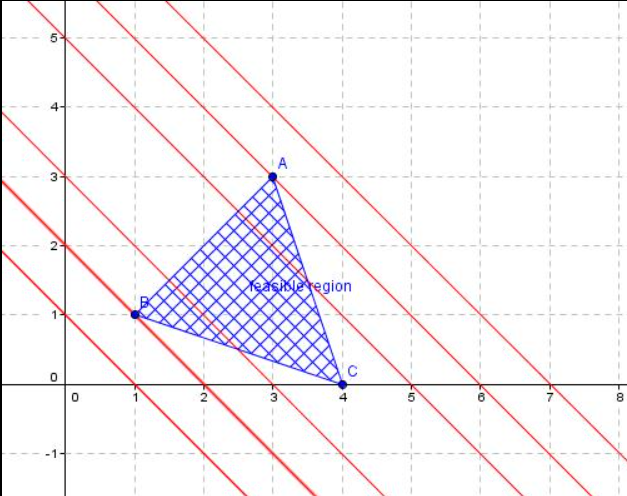
\includegraphics[width=0.4\textwidth]{_files/_images/18.png}
    \label{fig:mia_immagine}
\end{figure}


se scegliamo

$$
c=(1,1),
$$

la funzione è

$$
f(x_1,x_2)=x_1+x_2.
$$

Muovendosi nella direzione opposta a \(c\), la funzione diminuisce. Il primo e unico punto del poliedro raggiunto in questa direzione è il vertice \(B\); pertanto \(B\) è un vertice secondo la definizione.

Analogamente, scegliendo

$$
c=(0,3),
$$

la funzione diventa

$$
f(x_1,x_2)=3x_2.
$$

Le sue curve di livello sono rette orizzontali. Muovendosi nella direzione opposta a \(c\), cioè verso il basso, il valore della funzione diminuisce. In questo caso il punto \(C\) è l'unico punto del poliedro in cui la funzione raggiunge il valore minimo e, di conseguenza, anche \(C\) è un vertice.

Non sono nè \(B\) nè \(A\) perchè le loro \textbf{curve di livello hanno un valore maggiore}.

Quindi deve esistere una funzione tale che quel punto è il minimo ottimo, anche A e C che si trovano sullo stesso segmento possono essere vertici, basta scegliere la funzione opportuna

\subsection*{Notazione degli indici nei problemi di Programmazione Lineare}

Consideriamo un generico problema di Programmazione Lineare (PL) con
$n$ variabili decisionali

\[
x_1,x_2,\ldots,x_n
\]

e $m$ vincoli, indicizzati da

\[
i=1,\ldots,m.
\]

Gli indici vengono utilizzati per identificare in modo univoco i
vincoli e le variabili. In particolare, è importante distinguere gli
indici dei vincoli dagli indici delle variabili:

\[
\boxed{M=\text{insiemi di indici dei vincoli}}
\]

\[
\boxed{N=\text{insiemi di indici delle variabili}}
\]

\[
\begin{aligned}
\min \quad & c'x \quad \text{(P)} \\
\text{s.a} \quad & \\
& a'_i x \ge b_i \quad & i \in M_1 \\
& a'_i x \le b_i \quad & i \in M_2 \\
& a'_i x = b_i \quad & i \in M_3 \\
& x_j \ge 0 \quad & j \in N_1 \\
& x_j \le 0 \quad & j \in N_2 \\
& x_j \text{ non vincolata} \quad & j \in N_3
\end{aligned}
\]

\subsubsection*{Indici dei vincoli: $M_1,M_2,M_3$}

Gli insiemi $M_1,M_2,M_3$ sono insiemi di indici che permettono di
classificare i vincoli in base al tipo di relazione che presentano.

\begin{itemize}
    \item $M_1$ contiene gli indici dei vincoli di tipo $\ge$;
    \item $M_2$ contiene gli indici dei vincoli di tipo $\le$;
    \item $M_3$ contiene gli indici dei vincoli di tipo $=$.
\end{itemize}

Pertanto, quando scriviamo

\[
a_i^Tx\ge b_i
\qquad i\in M_1,
\]

stiamo dicendo che, per ogni indice $i$ appartenente all'insieme
$M_1$, il vincolo corrispondente è di tipo $\ge$.

Ad esempio, supponiamo di avere $5$ vincoli:

\[
\begin{aligned}
a_1^Tx &\ge b_1\\
a_2^Tx &\le b_2\\
a_3^Tx &= b_3\\
a_4^Tx &\ge b_4\\
a_5^Tx &\le b_5.
\end{aligned}
\]

In questo caso possiamo definire:

\[
M_1=\{1,4\},
\]

poiché i vincoli $1$ e $4$ sono di tipo $\ge$;

\[
M_2=\{2,5\},
\]

poiché i vincoli $2$ e $5$ sono di tipo $\le$;

\[
M_3=\{3\},
\]

poiché il vincolo $3$ è un'uguaglianza.

Quindi la scrittura compatta

\[
a_i^Tx\ge b_i
\qquad i\in M_1
\]

equivale, nell'esempio precedente, a scrivere

\[
\begin{cases}
a_1^Tx\ge b_1\\
a_4^Tx\ge b_4.
\end{cases}
\]

\textbf{Dove $a_i^T$} è l'intero vettore dell'$i-esimo$ vincolo.

Analogamente,

\[
a_i^Tx\le b_i
\qquad i\in M_2
\]

equivale a

\[
\begin{cases}
a_2^Tx\le b_2\\
a_5^Tx\le b_5,
\end{cases}
\]

mentre

\[
a_i^Tx=b_i
\qquad i\in M_3
\]

equivale a

\[
a_3^Tx=b_3.
\]

\subsubsection*{Indici delle variabili: $N_1,N_2,N_3$}

Gli insiemi $N_1,N_2,N_3$ svolgono un ruolo analogo, ma questa volta
si riferiscono alle \emph{variabili} e non ai vincoli.

Gli indici delle variabili sono

\[
j=1,\ldots,n.
\]

Gli insiemi $N_1,N_2,N_3$ classificano le variabili in base al
vincolo imposto sul loro segno:

\begin{itemize}
    \item $N_1$ contiene gli indici delle variabili non negative;
    \item $N_2$ contiene gli indici delle variabili non positive;
    \item $N_3$ contiene gli indici delle variabili non vincolate
    rispetto al segno.
\end{itemize}

In particolare,

\[
x_j\ge0
\qquad j\in N_1
\]

significa che, per ogni indice $j$ appartenente a $N_1$, la variabile
$x_j$ deve essere non negativa.

Ad esempio, se

\[
N_1=\{1,3,5\},
\]

allora

\[
x_1\ge0,\qquad x_3\ge0,\qquad x_5\ge0.
\]

Analogamente,

\[
x_j\le0
\qquad j\in N_2
\]

significa che le variabili i cui indici appartengono a $N_2$ devono
essere non positive.

Ad esempio, se

\[
N_2=\{2,6\},
\]

allora

\[
x_2\le0,\qquad x_6\le0.
\]

Infine,

\[
x_j\text{ non vincolata}
\qquad j\in N_3
\]

significa che le variabili i cui indici appartengono a $N_3$ non hanno
alcun vincolo sul segno. In altre parole,

\[
x_j\in\mathbb{R}.
\]

Una variabile non vincolata può quindi essere positiva, negativa
oppure nulla.

\subsubsection*{Differenza tra $M$ e $N$}

È importante ricordare la seguente distinzione:

\[
\boxed{
M_1,M_2,M_3
\longrightarrow
\text{insiemi di indici dei vincoli}
}
\]

\[
\boxed{
N_1,N_2,N_3
\longrightarrow
\text{insiemi di indici delle variabili}
}
\]

In particolare:

\[
\begin{array}{c|c|c}
\text{Insieme} & \text{Indici di} & \text{Significato}\\
\hline
M_1 & \text{vincoli} & \ge\\
M_2 & \text{vincoli} & \le\\
M_3 & \text{vincoli} & =\\
\hline
N_1 & \text{variabili} & x_j\ge0\\
N_2 & \text{variabili} & x_j\le0\\
N_3 & \text{variabili} & x_j\text{ libera}
\end{array}
\]

\subsubsection*{Esempio completo}

Supponiamo di avere $4$ variabili

\[
x_1,x_2,x_3,x_4
\]

e $5$ vincoli:

\[
\begin{aligned}
x_1+x_2&\ge2\\
2x_1-x_3&\le5\\
x_2+x_4&=3\\
x_1-x_4&\ge1\\
x_2+x_3&\le7.
\end{aligned}
\]

Dove ad esempio $a_1^T = (1,1,0,0)$ , $a_2^T = (2,,0-1,0)$ , $\dots$


Indicizziamo i vincoli con

\[
i=1,\ldots,5.
\]

I vincoli possono essere classificati nel seguente modo:

\[
M_1=\{1,4\},
\]

perché i vincoli $1$ e $4$ sono di tipo $\ge$;

\[
M_2=\{2,5\},
\]

perché i vincoli $2$ e $5$ sono di tipo $\le$;

\[
M_3=\{3\},
\]

perché il vincolo $3$ è di tipo $=$.

Supponiamo inoltre che le variabili soddisfino:

\[
x_1\ge0,\qquad
x_2\ge0,\qquad
x_3\le0,\qquad
x_4\in\mathbb{R}.
\]

In questo caso abbiamo:

\[
N_1=\{1,2\},
\]

perché $x_1$ e $x_2$ sono non negative;

\[
N_2=\{3\},
\]

perché $x_3$ è non positiva;

\[
N_3=\{4\},
\]

perché $x_4$ è una variabile non vincolata rispetto al segno.



\begin{definition}{Vincolo Attivo}
Se un vettore $x^*$ soddisfa $a_i^Tx^* = b_i$ per qualche $i \in M_1 \cup M_2 \cup M_3$, allora il corrispondente vincolo si dice \textit{attivo} in $x^*$.

Un vincolo sulla variabile $j \in N_1 \cup N_2$ si dice attivo in $x^*$ se la variabile assume valore nullo, ossia se:   $$x_j^* = 0$$


\end{definition}


\textbf{Esempio pratico}

Immaginiamo un problema con due variabili $x = \begin{pmatrix} x_1 \\ x_2 \end{pmatrix}$ e due vincoli di tipo $\le$:
\begin{enumerate}
    \item $x_1 + x_2 \le 10$
    \item $3x_1 + x_2 \le 15$
\end{enumerate}

Prendiamo un vettore specifico come punto di prova, ad esempio $x^* = \begin{pmatrix} 2 \\ 8 \end{pmatrix}$ (cioè $x_1 = 2$ e $x_2 = 8$). Sostituiamo questi valori all'interno dei vincoli per verificare se sono attivi:

\begin{itemize}
    \item \textbf{Analisi del Vincolo 1:}\\
    $$ 2 + 8 \le 10 \implies 10 = 10 $$
    L'equazione $a_1'x^* = b_1$ è perfettamente soddisfatta. Il punto esaurisce esattamente il termine noto. Pertanto, \textbf{il vincolo 1 è attivo in $x^*$}.

    \item \textbf{Analisi del Vincolo 2:}\\
    $$ 3(2) + 8 \le 15 \implies 6 + 8 \le 15 \implies 14 \le 15 $$
    L'equazione $a_2'x^* = b_2$ non è soddisfatta perché $14 \neq 15$. C'è uno scarto rispetto al limite. Pertanto, \textbf{il vincolo 2 NON è attivo in $x^*$} (è un vincolo "lasco" o inattivo).
\end{itemize}

\clearpage

Se $x^*$ attiva $n$ vincoli (\textbf{cioè gli stessi della sua dimensione}), allora $x^*$ soddisfa un certo \textbf{sistema di $n$ equazioni} lineari in $n$ incognite.
Questo sistema ha un'unica soluzione, se e solo se le $n$ \textbf{equazioni}, sono \textbf{linearmente indipendenti}.
Il seguente teorema da un preciso significato a questa affermazione


\begin{example}{Vincoli attivi e sistema di equazioni}

Consideriamo un problema di Programmazione Lineare con $n=2$ variabili
e supponiamo che, in un punto $x^*$, siano attivi i seguenti due
vincoli:

\[
\begin{cases}
x_1+x_2\le3\\
x_1-x_2\le-1.
\end{cases}
\]

Poiché entrambi i vincoli sono attivi in $x^*$, devono essere
soddisfatti con uguaglianza:

\[
\begin{cases}
x_1+x_2=3\\
x_1-x_2=-1.
\end{cases}
\]

Abbiamo quindi un sistema di $n=2$ equazioni lineari in $n=2$
incognite.

La matrice dei coefficienti è

\[
A=
\begin{pmatrix}
1 & 1\\
1 & -1
\end{pmatrix}.
\]

Le due equazioni sono linearmente indipendenti, poiché i vettori

\[
(1,1)
\qquad\text{e}\qquad
(1,-1)
\]

non sono multipli l'uno dell'altro.

Infatti,

\[
\det(A)
=
\begin{vmatrix}
1 & 1\\
1 & -1
\end{vmatrix}
=-2\neq0.
\]

Pertanto il sistema ammette un'unica soluzione:

\[
\begin{cases}
x_1+x_2=3\\
x_1-x_2=-1
\end{cases}
\quad\Longrightarrow\quad
x^*=
\begin{pmatrix}
1\\
2
\end{pmatrix}.
\]

Quindi i due vincoli attivi e linearmente indipendenti determinano
un unico punto $x^*$.

\medskip

Al contrario, se i due vincoli attivi fossero

\[
\begin{cases}
x_1+x_2\le3\\
2x_1+2x_2\le6,
\end{cases}
\]

avremmo il sistema

\[
\begin{cases}
x_1+x_2=3\\
2x_1+2x_2=6.
\end{cases}
\]

In questo caso le due equazioni sono linearmente dipendenti, poiché
la seconda è il doppio della prima. Pertanto il sistema non determina
un'unica soluzione, ma ammette infinite soluzioni.

\[
\boxed{
\text{Per determinare un unico punto sono necessari $n$ vincoli attivi
linearmente indipendenti.}
}
\]

\end{example}

\begin{theorem}{Teorema}
Sia $x^* \in \mathbb{R}^n$ e sia $I = \{i \mid a^T_i x^* = b_i\}$ l'insieme degli indici dei vincoli che sono attivi in $x^*$. Allora, le seguenti affermazioni sono equivalenti fra loro:

\begin{itemize}
    \item $n$ vettori nell'insieme $\{a_i \mid i \in I\}$ sono linearmente indipendenti;
    
    (\textbf{Nota che però qui non stiamo dicendo che ci saranno sempre $n$ vettori linearmente indipendenti, MA CHE QUANDO CI SONO, allora c'è un uguaglianza logica fra queste tre punti})

    \item $\{a_i \mid i \in I\}$ (l'insieme di vettori l.indipendenti del punto di sopra) è una base di $\mathbb{R}^n$, cioè ogni elemento di $\mathbb{R}^n$ può essere espresso come combinazione lineare dei vettori $a_i, \ i \in I$;
    
    \item il sistema di equazioni $a^T_i x = b_i, \ i \in I$, ha un'unica soluzione e quella soluzione è $x^*$
\end{itemize}
\end{theorem}

Ora abbiamo tutti gli strumenti per definire un vertice di un poliedro come \textit{soluzione ammissibile che attiva $n$ vincoli linearmente indipendenti} (cioè la terza definizione uguale a quella
di vertice e punto di estremo):

\begin{definition}{Soluzione di Base e Soluzione di Base Ammissibile}
Sia $P$ un poliedro definito da vincoli di uguaglianza e/o disuguaglianza come nel problema $(P)$ e sia $x^* \in \mathbb{R}^n$.
\begin{itemize}[label=$\bullet$, leftmargin=2em]
    \item Il vettore $x^*$ è una \textbf{soluzione di base} se:
    \begin{itemize}[label=--, leftmargin=1.5em]
        \item tutti i vincoli di uguaglianza (e si parla solo dei vincoli di uguaglianza) di $(P)$ sono attivi in $x^*$;
        \item $x^*$ attiva $n$ vincoli linearmente indipendenti.
    \end{itemize}
    \item Se $x^*$ è una soluzione di base che soddisfa tutti i vincoli di $(P)$, allora $x^*$ è detta \textbf{soluzione di base ammissibile} (SBA).
\end{itemize}
\end{definition}

\begin{example}{Soluzione di base e soluzione di base ammissibile}

Consideriamo il poliedro

$$
P = \left\{x \in \mathbb{R}^2 \mid
\begin{cases}
x_1 + x_2 \leq 4\\
x_1 \geq 0\\
x_2 \geq 0
\end{cases}
\right\}.
$$

Una \emph{soluzione di base} è un punto che soddisfa un sistema formato da $n=2$ vincoli linearmente indipendenti presi tra i vincoli del problema, considerando come uguaglianze i vincoli attivi.

\medskip

Consideriamo, ad esempio, il punto

$$
x^* =
\begin{pmatrix}
4\\
0
\end{pmatrix}.
$$

Nel punto $x^*$ sono attivi i vincoli

$$
x_1+x_2=4
\qquad\text{e}\qquad
x_2=0.
$$

Essi formano il sistema

$$
\begin{cases}
x_1+x_2=4\\
x_2=0
\end{cases}
$$

le cui due equazioni sono linearmente indipendenti e determinano un'unica soluzione:

$$
x^*=(4,0).
$$

Pertanto $x^*$ è una \emph{soluzione di base}.

Inoltre, $x^*$ soddisfa anche tutti i vincoli del poliedro:

$$
4+0\leq4,\qquad 4\geq0,\qquad 0\geq0.
$$

Quindi

$$
x^*=(4,0)
$$

è una \emph{soluzione di base ammissibile}.

\medskip

Consideriamo invece il punto

$$
\bar{x}=
\begin{pmatrix}
4\\
-1
\end{pmatrix}.
$$

In $\bar{x}$ sono attivi i vincoli

$$
x_1+x_2=3
$$

e, in realtà, nessun altro vincolo del poliedro è attivo. Quindi non abbiamo $2$ vincoli attivi linearmente indipendenti e $\bar{x}$ non è una soluzione di base.
\end{example}

\subsection{Interpretazione Geometrica: Corrispondenza con i Vertici}

L'idea fondamentale è che, in uno spazio $\mathbb{R}^n$, un sistema costituito da $n$ equazioni lineari indipendenti individua un unico punto.

Esiste quindi una fondamentale corrispondenza tra l'algebra della Programmazione Lineare e la geometria dei poliedri:

\begin{center}
\textbf{Un punto $x^* \in P$ è una Soluzione di Base Ammissibile (SBA) $\iff$ $x^*$ è un vertice (punto estremo) di $P$.}
\end{center}

Questo perché una soluzione di base è determinata dall'attivazione di \(n\) vincoli linearmente indipendenti. In uno spazio \(\mathbb{R}^n\), tali vincoli identificano un unico punto, come intersezione degli \(n\) iperpiani corrispondenti. Il punto soddisfa quindi le uguaglianze associate ai vincoli attivi e si troverà sull'intersezione di questi iperpiani.
Quindi si troverà ai "bordi", dato che si trova sugli iperpiani.

Se, inoltre, questo punto è ammissibile, allora appartiene all'insieme ammissibile (il poliedro) e, di conseguenza, è un vertice del poliedro, poiché è individuato dall'intersezione di \(n\) vincoli linearmente indipendenti.

\subsubsection{Perché una SBA identifica un vertice?}

Per comprendere intuitivamente questa corrispondenza, consideriamo prima il caso bidimensionale, cioè $\mathbb{R}^2$.

\begin{enumerate}

\item \textbf{Vincoli e rette di frontiera:}

Ogni vincolo di disuguaglianza lineare
\[
a_i^T x \leq b_i
\]
individua un semispazio. La sua frontiera è la retta
\[
a_i^T x = b_i.
\]

\item \textbf{Vincoli attivi e intersezione:}

Un vincolo si dice \emph{attivo} in $x^*$ quando è soddisfatto con l'uguaglianza:
\[
a_i^T x^* = b_i.
\]

In $\mathbb{R}^2$, se $x^*$ attiva due vincoli i cui vettori normali $a_i$ e $a_j$ sono linearmente indipendenti, le corrispondenti rette non sono parallele e si intersecano in un unico punto.

Pertanto, il sistema
\[
\begin{cases}
    a_i^T x = b_i\\
    a_j^T x = b_j
\end{cases}
\]
individua un unico punto $x^*$.

\item \textbf{Ammissibilità:}

Il punto di intersezione non è necessariamente un vertice del poliedro. Bisogna verificare che esso soddisfi anche tutti gli altri vincoli che definiscono $P$.

\begin{itemize}
    \item Se il punto non soddisfa tutti i vincoli, allora è una \emph{soluzione di base non ammissibile}.
    \item Se il punto soddisfa tutti i vincoli, allora $x^* \in P$ e rappresenta un \emph{vertice} del poliedro.
\end{itemize}

\end{enumerate}

\begin{center}
    Una soluzione di base (\textbf{non ammissibile}) rappresenta invece, un'intersezione di rette lineramente indipendenti, che però non sono nella regione ammissibile.
\end{center}


\begin{figure}[htbp]
    \centering
    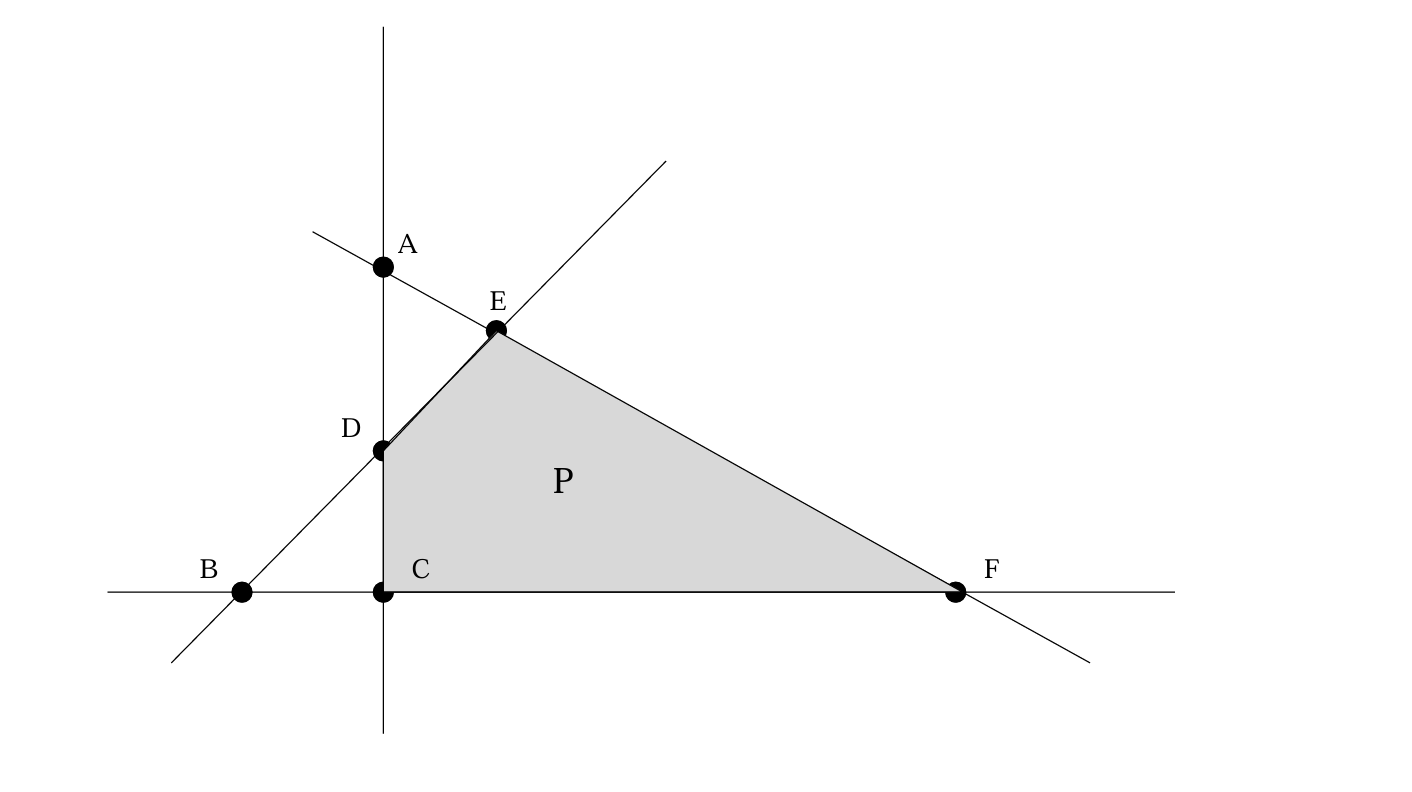
\includegraphics[width=0.6\textwidth]{_files/_images/19.png}
    \label{fig:mia_immagine}
\end{figure}
Nell'esempio sopra, $A$ e $B$, sono soluzioni di base, ma non ammissibili, questo perchè non sono nel poliedro, però soddisfano sempre $n$ equazioni linearmente indipendenti (una è quello della retta e una sarà quella della condizione sulle variabili, cioè che una componente è uguale a 0, o comunque basta guardare il grafico).
Se soddisfano tutti i vincoli del poliedro, invece staranno nel poliedro (come $E$, $D$,...)

\begin{theorem}{Equaglianza fra definizioni}
    Sia $P$ un poliedro non vuoto e sia $x^* \in P$. Le seguenti tre affermazioni sono equivalenti:
    \begin{itemize}
        \item $x^*$ è un vertice di $P$;
        \item $x^*$ è un punto estremo di $P$;
        \item $x^*$ è una soluzione di base ammissibile.
    \end{itemize}
\end{theorem}

\begin{corollary}{Corollario}
    Dato un numero finito di vincoli lineari di disequazioni e/o equazioni, pu`o esistere solo un numero finito di soluzioni di base e soluzioni di base ammissibili. 
\end{corollary}


\begin{definition}{Soluzioni di base adiacenti}
Due distinte soluzioni di base di un poliedro $P \subseteq \mathbb{R}^n$ si dicono \textbf{adiacenti} se attivano gli stessi $n - 1$ vincoli. 

Se due soluzioni di base adiacenti sono anche ammissibili, allora il segmento che le congiunge è detto \textbf{lato} (o \textbf{spigolo}) del poliedro.
\end{definition}
\begin{example}{Soluzione di base adiacente}
    Nel seguente esempio
    \begin{center}
        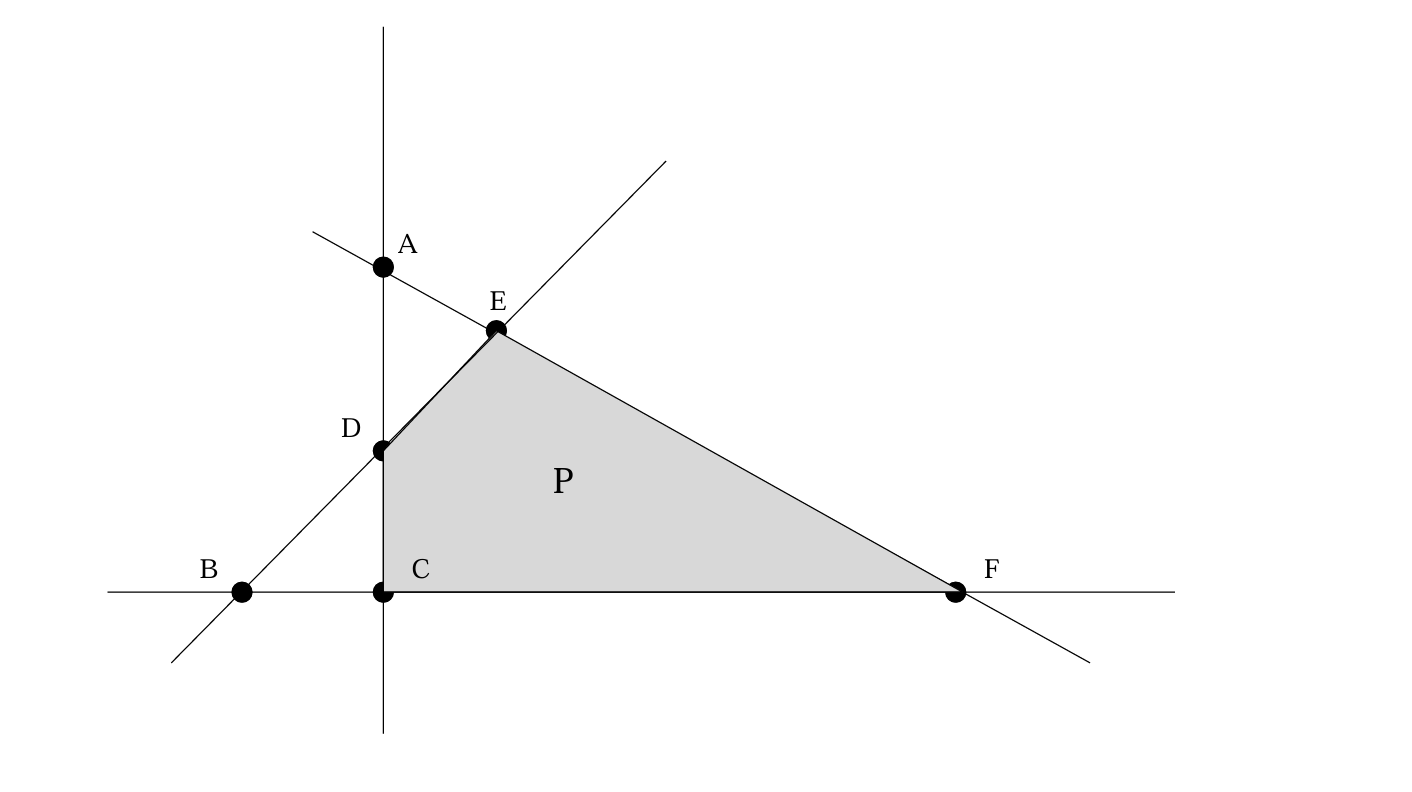
\includegraphics[width=0.7\linewidth]{_files/_images/19.png}
    \end{center}
    \begin{itemize}
        \item $B$ e $D$ sono adiacenti.
        \item $B$ e $E$ sono adiacenti.
        \item $D$ e $E$ sono adiacenti.
    \end{itemize}
\end{example}

\section{Poliedri in Forma Standard}
Sia $P$ = \{$x \in \mathbb{R}^n$ | $Ax = b$ , $x$ >= 0\} un poliedro rappresentato in forma standard.
Abbiamo già osservato in precedenza che senza
perdita di generalità è possibile assumere che m < n e che gli m vincoli
siano linearmente indipendenti.

Un poliedro in forma standard geometricamente, può rappresentare varie cose:

\begin{enumerate}
    \item Se siamo in $\mathbb{R}^2$, e abbiamo $m$ = 1 vincolo di uguaglianza, allora il poliedro è una retta.
    \begin{figure}[htbp]
        \centering
        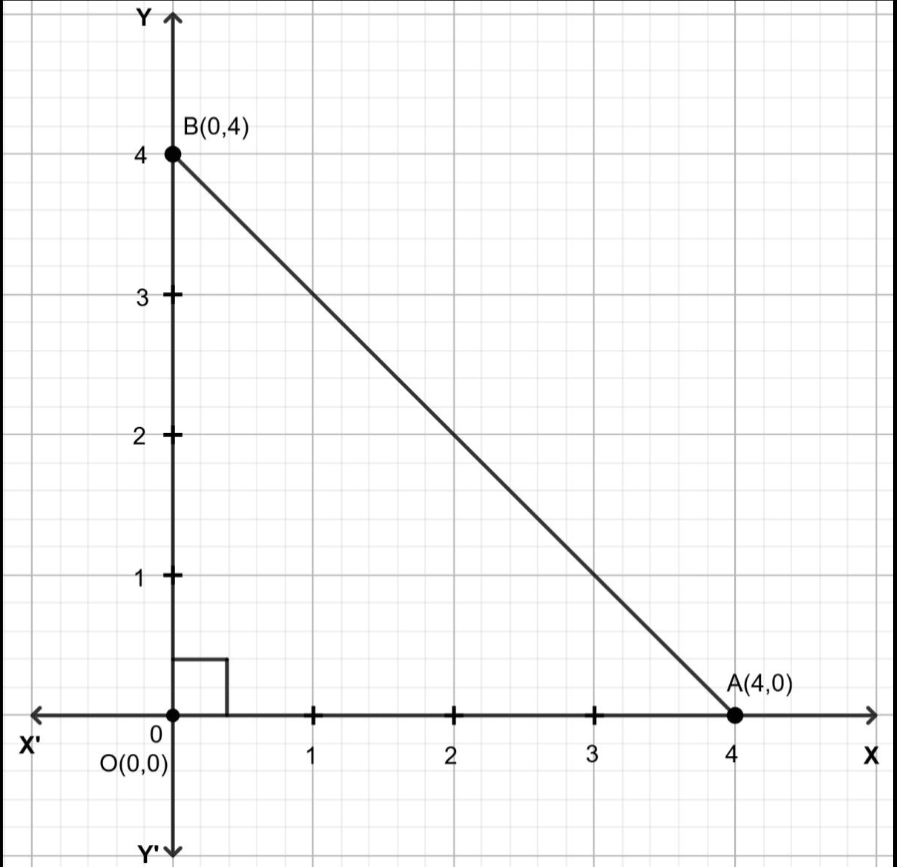
\includegraphics[width=0.4\textwidth]{_files/_images/20.png}
        \caption{Il vincolo $x_1 + x_2 = 4$ identifica una retta, con i due ulteriori non vincoli di uguaglianza $x_1 >= 0$ e $x_2 >= 0$, si ha quello in foto}
        \label{fig:mia_immagine}
    \end{figure}
    \item Se siamo in $\mathbb{R}^2$, e abbiamo $m$ = 2 vincoli di uguaglianza, lineramente indipendenti (come da ipotesi), allora l'interesezione fra questi due è un punto.
    Supponiamo di avere:
    \[
    \begin{cases}
    x_1+x_2=4\\
    x_1-x_2=0\\
    x_1,x_2\geq 0
    \end{cases}
    \]
    Allora graficamente si ha:
    \begin{figure}[htbp]
        \centering
        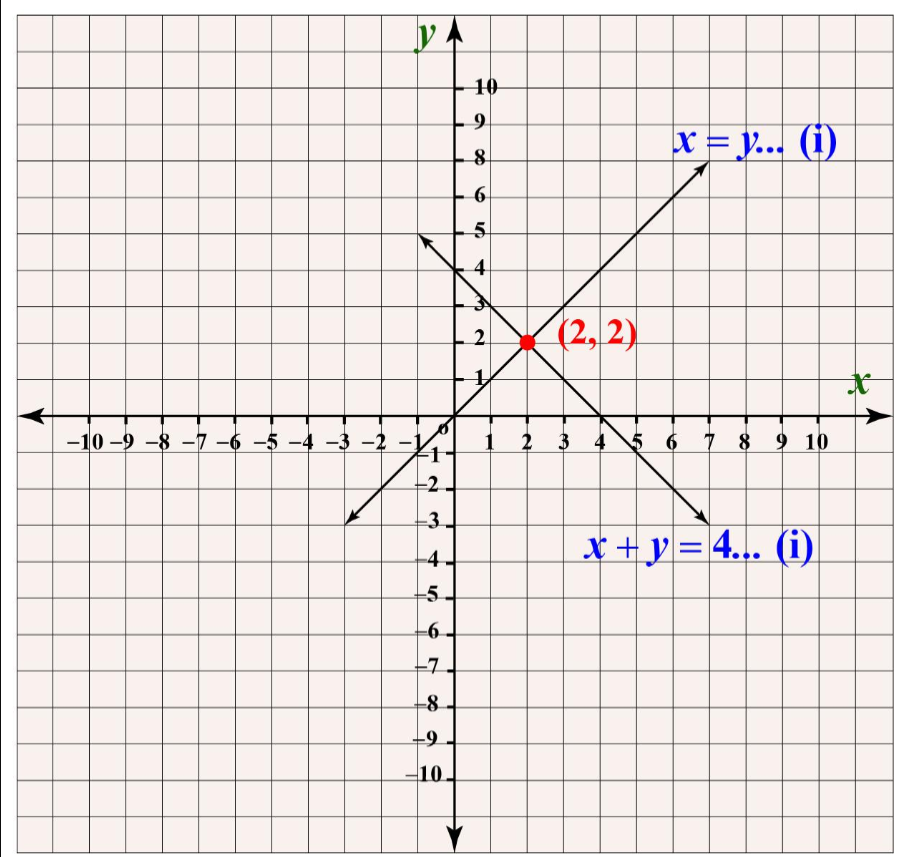
\includegraphics[width=0.4\textwidth]{_files/_images/21.png}
        \caption{L'intersezione di due rette lineramente indipendenti va a formare un punto in $\mathbb{R}^2$}
        \label{fig:mia_immagine}
    \end{figure}
    \item In $\mathbb{R}^2$, posso rappresentare anche un'area, quello che si fa è \textbf{non avere vincoli}, ma solo quelli della positività sulle variabili:
    Se abbiamo soltanto $x_1\geq 0$ e $x_2\geq 0$, otteniamo tutto il primo quadrante, che è una regione bidimensionale.
    \item Se siamo in $\mathbb{R}^3$ (quindi 3 variabili) e $m$ = 2 uguaglianze:
    \[
    \begin{cases}
    x_1+x_2+x_3=4\\
    x_1-x_2=0\\
    x_1,x_2,x_3\geq0
    \end{cases}
    \]
    Qui non rappresentiamo un punto, perchè abbiamo $m$ = 2 equazioni, ma $n$ = 3 variabili.
    In questo caso $x_1 - x_2 = 0$ rappresenta un piano, perchè lo vedi come $x_1 - x_2 + 0 x_3 = 0$ quindi va bene qualsiasi valore di $x_3$
    \begin{figure}[htbp]
        \centering
        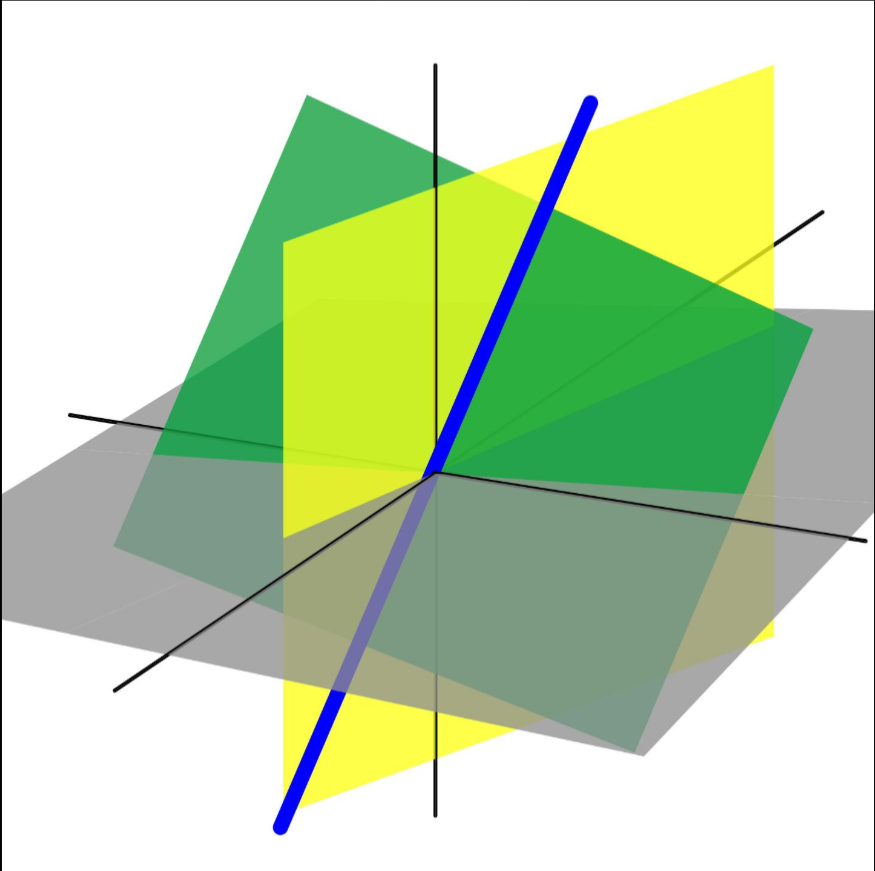
\includegraphics[width=0.4\textwidth]{_files/_images/22.png}
        \caption{L'intersezione di due piani non paralleli è una retta}
        \label{fig:mia_immagine}
    \end{figure}
    In $\mathbb{R}^3$, ciascuna uguaglianza rappresenta un piano. L'intersezione di due piani non paralleli è generalmente una retta.
\end{enumerate}

\newpage

Ora nota che $x = 0$ in $\mathbb{R}^2$, indica una retta:
\begin{figure}[htbp]
        \centering
        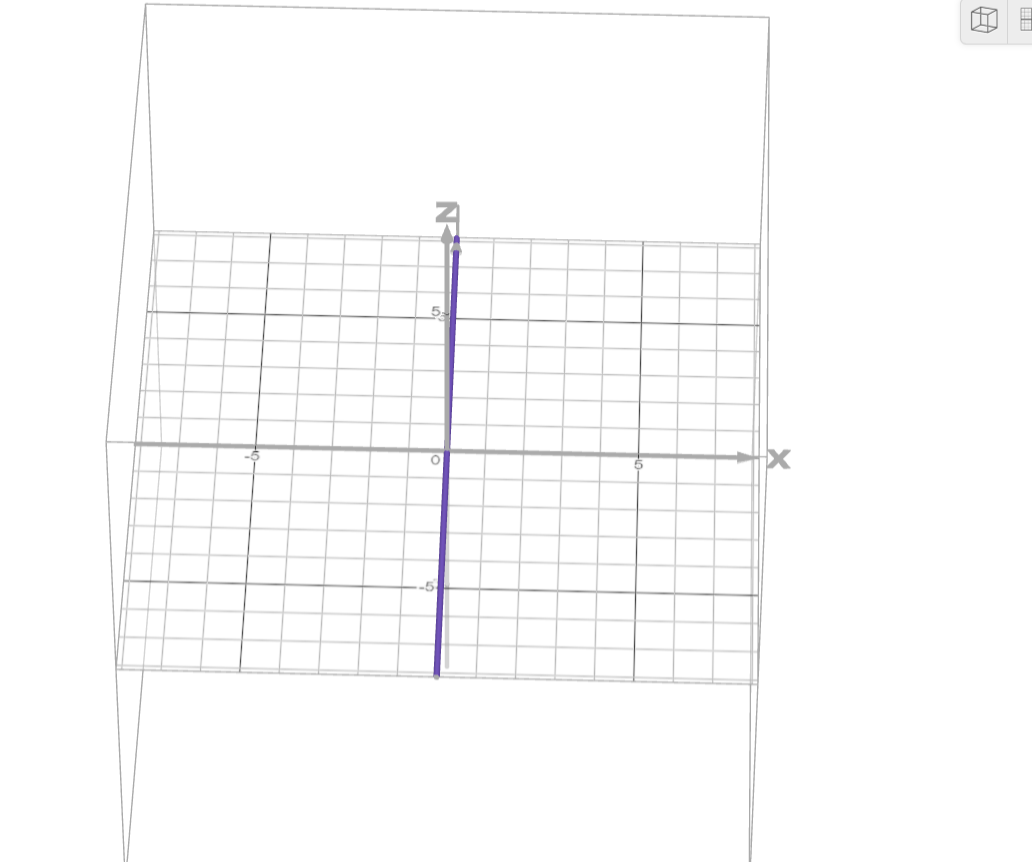
\includegraphics[width=0.4\textwidth]{_files/_images/23.png}
        \caption{Retta individuata da $x$ = 0, questo perchè lo puoi pensare come $x + 0 * y = 0$, quindi $y$ può assumere qualsiasi valore}
        \label{fig:mia_immagine}
\end{figure}

\newpage

In $\mathbb{R}^3$, indica un piano:
\begin{figure}[htbp]
        \centering
        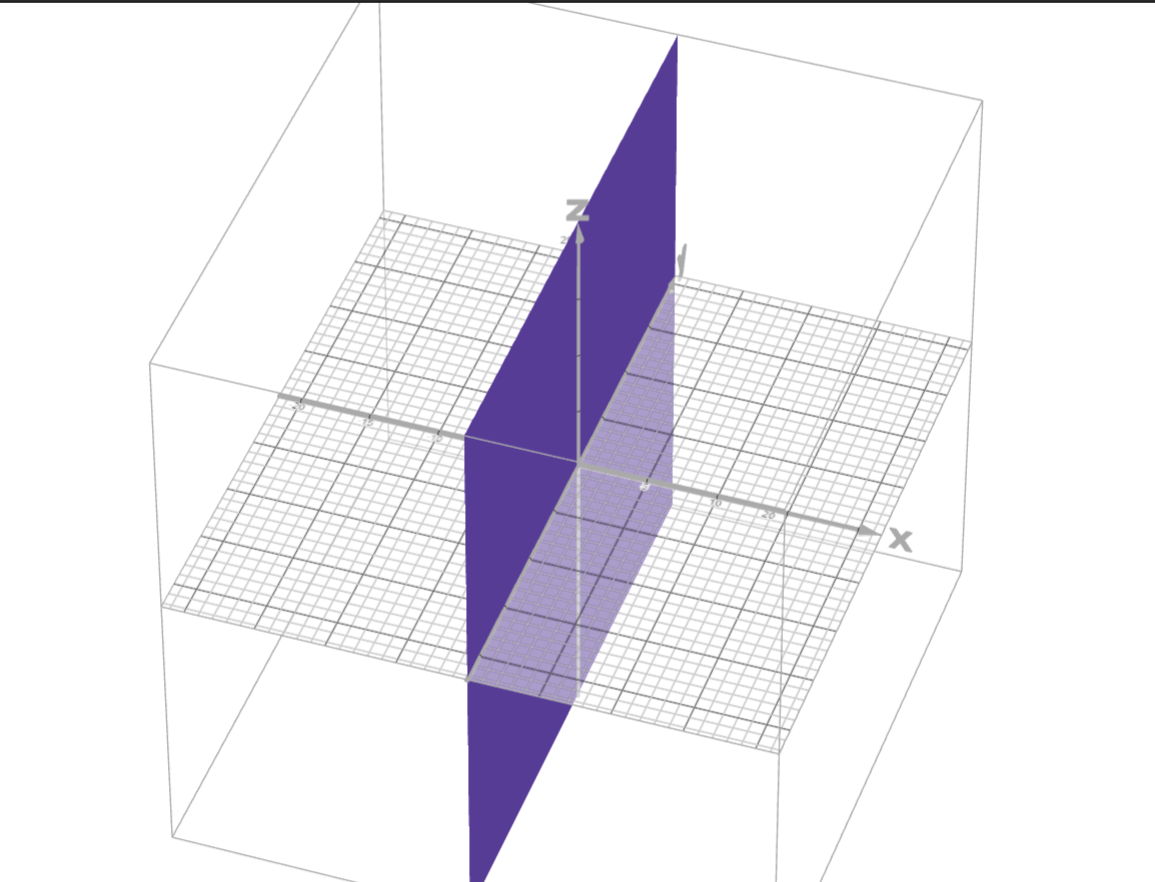
\includegraphics[width=0.4\textwidth]{_files/_images/24.png}
        \caption{Piano individuata da $x$ = 0, questo perchè lo puoi pensare come $x + 0 * y + 0 * z= 0$, quindi $y$ e $z$ possono assumere qualsiasi valore}
        \label{fig:mia_immagine}
\end{figure}

In $\mathbb{R}^3$, si può anche identificare un "triangolo" tramite il sistema:
\[
\begin{cases}
    x + y + z = 4,\\
    x \ge 0,\\
    y \ge 0,\\
    z \ge 0.
\end{cases}
\]
Il sistema descrive un triangolo in $\mathbb{R}^3$. Come puoi vedere, alcuni punti non corrispondono al triangolo perché non rispettano i vincoli del piano e delle variabili. Se dovessi trasformare $z$ (come quando faccio $y = x - 2$) in una funzione, il suo dominio diverrebbe
$$D = \{ (x, y) \in \mathbb{R}^2 \mid x \ge 0, \, y \ge 0, \, x + y \le 4 \}$$
\begin{figure}[htbp]
        \centering
        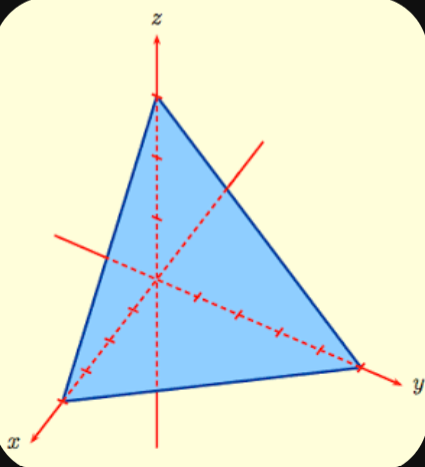
\includegraphics[width=0.4\textwidth]{_files/_images/27.png}
        \caption{Triangolo individuato in blu (fra me e me, sotto non c'è niente)}
        \label{fig:mia_immagine}
\end{figure}

\newpage

Abbiamo definito una **soluzione di base** come un punto che rende attivi \(n\) vincoli linearmente indipendenti.

Nel caso di un poliedro in forma standard, oltre agli \(m\) vincoli di uguaglianza, che sono linearmente indipendenti per ipotesi, per ottenere un totale di \(n\) vincoli attivi linearmente indipendenti, è necessario individuare \(n-m\) variabili di decisione \(x_j\) da porre uguali a zero, in modo da rendere attivi i corrispondenti vincoli di non negatività \(x_j\geq 0\).

Questo perché, per identificare una soluzione di base, dobbiamo individuare \(n\) vincoli attivi linearmente indipendenti. Poiché gli \(m\) vincoli di uguaglianza sono già attivi, dobbiamo attivare altri \(n-m\) vincoli, imponendo che le corrispondenti variabili siano uguali a zero.

Dal punto di vista geometrico, ciascun vincolo \(x_j=0\) identifica un iperpiano in \(\mathbb{R}^n\). Imponendo contemporaneamente le \(m\) equazioni originali e le ulteriori \(n-m\) equazioni introdotte, otteniamo un sistema di \(n\) equazioni lineari.

Affinché questi vincoli individuino un unico punto, è necessario che siano complessivamente linearmente indipendenti.

La scelta delle \(n-m\) variabili di decisione da porre uguali a zero, tuttavia, non è del tutto arbitraria: i corrispondenti vincoli devono essere linearmente indipendenti sia tra loro sia rispetto agli \(m\) vincoli di uguaglianza originali. Inoltre, affinché il punto individuato sia una soluzione di base ammissibile, deve soddisfare tutti i vincoli del poliedro.

Queste considerazioni sono formalizzate dal seguente teorema.

\begin{center}
    Nel lungo procedimento che vedremo di seguito, si andranno a scegliere quali dei vincoli di $j$, saranno da mettere uguali a 0.
    Una volta fatto, poi si risolverà il sistema.
\end{center}


\begin{theorem}{Teorema}
    Si considerano i vincoli $Ax = b$ e $x$ >= 0 e si assuma che $A \in \mathbb{R}^{m \times n}$ sia una matrice a righe lineramente indipendenti (bisogna avere questi vincoli per applicare il teorema).
    Un vettore $x^* \in \mathbb{R}^n$ è soluzione di base se e solo se:
    \begin{itemize}
        \item $A x^* = b;$ (questo dalla definizione di soluzione di base, dove tutti i vincoli di uguaglianza devono essere soddisfatti)
        \item è possibile individuare $B(1),B(2),\dots,B(m)$ indici tali che:
        \begin{enumerate}
            \item le colonne $A_{B(1)},A_{B(2)},\dots,A_{B(m)}$ sono lineramente indipendenti;
            \item se $j$ != $B(1),B(2),\dots,B(m)$, allora $x^*_j$ = 0
        \end{enumerate}
    \end{itemize}
\end{theorem}
\label{teorema SBA}
Quello appena descritto si può descrivere in modo algoritmico in questo modo:
\begin{center}
\fbox{\parbox{0.9\linewidth}{
    \textbf{Passo 1.}\\
        Scegliere $m$ colonne di $A$ lineramente indipendenti. \\
        Siano $A_{B(1)},A_{B(2)},\dots,A_{B(m)}$ dette colonne. \\
    \textbf{Passo 2.}\\
        Porre $x_j$ = 0, per ogni $j$ != $B(1),B(2),\dots,B(m)$ \\
    \textbf{Passo 3.}\\
        Risolvere il sistema ad $m$ equazioni $Ax = b$ nelle $m$ incognite $x_{B(1)},x_{B(2)},\dots,x_{B(M)}$, perchè le altre $n - m$ incognite saranno messe a 0 dal passo 2.
}}
\end{center}
Facciamo un esempio per chiarire,consideriamo il sistema:
\[
\begin{cases}
x_1+x_2+x_3=4\\
2x_1+x_2+x_3=5\\
x_1,x_2,x_3\geq 0
\end{cases}
\]
La matrice dei coefficienti è:
\[
A=
\begin{pmatrix}
1&1&1\\
2&1&1
\end{pmatrix},
\qquad
b=\begin{pmatrix}4\\5\end{pmatrix}.
\]

\paragraph{Passo 1 : Scegliere \(m\) colonne linearmente indipendenti}
La matrice \(A\) ha \(m=2\) righe e \(n=3\) colonne. Dobbiamo quindi scegliere due colonne linearmente indipendenti.
Scegliamo la prima e la seconda colonna:
\[
A_{B(1)}=\begin{pmatrix}1\\2\end{pmatrix},
\qquad
A_{B(2)}=\begin{pmatrix}1\\1\end{pmatrix}.
\]

Dove $B(1)$ = 1 e $B(2)$ = 2
La matrice formata dalle colonne scelte è:
\[
B=\begin{pmatrix}
1&1\\
2&1
\end{pmatrix}.
\]
Questa matrice è chiamata matrice di base, $B \in \mathbb{R}^{m \times m}$.


\textbf{Nota: Si può sempre modificare la matrice originale A, in modo che le colonne lineramente indipendenti $A_{B(1)}...$ siano tutte vicine, quindi ottenere gli indici che partono da 1 e sono tutti attaccati} e quindi ottenere una sottomatrice $B$,

\paragraph{Passo 2: Porre le variabili uguali a 0}
Ora dobbiamo porre $j$ uguale a 0, ma quale $j$?
abbiamo che B(1) = 1 e B(2) = 2, quindi $x_3$ = 0.

Le variabili $x_{B(1)},x_{B(2)}$ sono chiamate \textbf{variabili di base, mentre $x_3$ è una variabile non di base}.


\textbf{Attenzione}: non stiamo ponendo a zero tutte le variabili, ma soltanto quelle che non corrispondono alle colonne scelte al Passo 1.

Quindi l'algoritmo troverà che la variabile $j$ da mettere uguale a 0, sarà $x_3$.
Quindi si risolverà il sistema di $m$ equazioni originali, aggiungendo l'equazione $x_3 = 0$,il sistema però non sarà come era originariamente in $n$ incognite, ma in $m$ cioè le incognite che non sono state messe a zero dall'algoritmo, cioè $x_{B(1)},x_{B(2)},\dots,x_{B(m)}$.
Quindi noi avevamo $n$ incognite iniziali, $m$ sono state scelte dall'algoritmo, e le restanti $n - m$ sono state messe a zero.

\paragraph{Passo 3 : Risolvere il sistema nelle variabili di base}
Sostituiamo \(x_3=0\) nel sistema originale:
\[
\begin{cases}
x_1+x_2+0=4\\
2x_1+x_2+0=5
\end{cases}
\]

\textbf{NOTA: Dato che ora non ci sono i vincoli $x_1$ e $x_2$ sono >= 0, la soluzione di base trovata non è detto sarà ammissibile.}

Otteniamo:
\[
\begin{cases}
x_1+x_2=4\\
2x_1+x_2=5
\end{cases}
\]

Sottraendo la prima equazione dalla seconda:
\[
x_1=1.
\]

Sostituendo nella prima equazione:
\[
1+x_2=4
\quad\Longrightarrow\quad x_2=3.
\]

Pertanto, la soluzione di base ottenuta è:
\[
\boxed{x^*=(1,3,0)}
\]
Poiché tutte le componenti sono non negative, questa è anche una soluzione di base ammissibile.
\begin{center}
    Questa è una soluzione di base,perchè mettendo la variabile $x_3$ = 0, si hanno $n$ vincoli lineramente indipendenti, e risolvendo il sistema si ha una soluzione che rispetta i vincoli $m$ originali (come vuole la definizione)
    piu i restanti vincoli sempre lineramente indipendenti fra di loro, ma che ne sono $n$ in totale, e quindi identificano un punto.
    \textbf{Quindi questo teorema è un se e solo se, nella direzione da destra verso sinistra, noi possiamo costruire una SBA, facendo questo procedimento descritto finora, e questa SBA, sarà costituita da:}
    \begin{itemize}
        \item \textbf{$x_B$} : che sarà fatto dalle variabili che non sono state messe a zero. Ha dimensione ($m$), e contiene i valori delle \(m\) variabili di base che, insieme alle variabili fuori base poste a zero, soddisfano tutti gli \(m\) vincoli di uguaglianza del sistema originale.
        \item \textbf{$x_N$} : che sarà fatto dalle variabili messe a zero ($n-m$), per soddisfare i vincoli originali
    \end{itemize}
\end{center}



Due matrici di base sono dette distinte se coinvolgono due insiemi di colonne linearmente indipendenti distinte.

Si noti che la matrice di base $B$ è invertibile essendo costituita da colonne lineramente indipendenti.

Analogamente possiamo costruire un vettore $x_B$ di variabili di decisione di base $x_{B(1)},x_{B(2)},\dots,x_{B(m)}$ ed un vettore $x_N$ di variabili di decisione non di base $x_j$
con $j != B(1),B(2),\dots,B(m)$ :
\begin{center}
$B = [A_{B(1)},A_{B(2)},\dots,A_{B(m)}]$, \\
$x_B$ = [$x_{B(1)}$ \\ $x_{B(2)}$ \\ \dots \\ $x_{B(m)}$].
\end{center}

Le variabili di decisione di base sono determinate risolvendo il sistema di $m$ equazioni in $m$ incognite.
Quindi in generale risolvere il sistema al \textbf{passo 3}, equivale a risolvere:
\begin{equation}
    B x_B = b
\end{equation}
la cui unica soluzione è data da:
\begin{equation}
    x_B = B^{-1} b
\end{equation}

\paragraph{Esempio}Sia $P$ il poliedro in forma standard descritto dai seguenti vincoli di uguaglianza lineari:
\begin{alignat*}{7}
x_1 & + {} & x_2 & + {} & 2x_3 & + {} & x_4 &      &     &      &     &      &     & = 8 \\
    &      & x_2 & + {} & 6x_3 & + {} &     & {} + & x_5 &      &     &      &     & = 12 \\
x_1 &      &     &      &      &      &     & {} + &     & {} + & x_6 &      &     & = 4 \\
    &      & x_2 &      &      &      &     &      &     & {} + &     & {} + & x_7 & = 6
\end{alignat*}
Dunque, la matrice $A$ e il vettore $b$, sono i seguenti:
\[
A = \begin{bmatrix}
1 & 1 & 2 & 1 & 0 & 0 & 0 \\
0 & 1 & 6 & 0 & 1 & 0 & 0 \\
1 & 0 & 0 & 0 & 0 & 1 & 0 \\
0 & 1 & 0 & 0 & 0 & 0 & 1
\end{bmatrix},
\]

\[
b = \begin{bmatrix}
8 \\
12 \\
4 \\
6
\end{bmatrix}.
\]
Scegliamo le colonne $A_4, A_5, A_6, A_7$, come colonne di base. Si noti che esse sono sicuramente linearmente indipendenti, in quanto $B = \begin{bmatrix} A_4 & A_5 & A_6 & A_7 \end{bmatrix}$ è la matrice identità.
Con tale scelta di matrice di base si deve risolvere:
\[
B x_B = b , \text{ dove }  x_B = \begin{bmatrix}
x_4 \\
x_5 \\
x_6 \\
x_7
\end{bmatrix}.
\]
Si ha che $x_1$, $x_2$, $x_3$ = 0 (quindi si raggiungono le 7 equazioni nel sistema), quindi:
\[
x_N = \begin{bmatrix}
x_1 \\
x_2 \\
x_3
\end{bmatrix}.
\]
e 
\[
x_B = \begin{bmatrix}
8 \\
12 \\
4 \\
6
\end{bmatrix}.
\]
Fondendo queste soluzioni si ha una soluzione di base ammissibile.

\begin{observation}{Il sistema $Ax = b$ può essere riscritto in altro modo}
Consideriamo un problema di programmazione lineare in forma standard:
\[
Ax=b,\qquad x\geq 0
\]

Dove:
- \(A\in\mathbb{R}^{m\times n}\) è la matrice dei coefficienti.
- \(x\in\mathbb{R}^n\) è il vettore delle variabili.
- \(b\in\mathbb{R}^m\) è il vettore dei termini noti.
Supponiamo di aver selezionato una base \(B\), costituita da \(m\) colonne linearmente indipendenti di \(A\).

Possiamo suddividere il sistema in:
\[
\boxed{Bx_B+Nx_N=b}
\]

dove \(x_B\) contiene le variabili di base e \(x_N\) quelle fuori base.
Consideriamo il sistema originale:
\[
\begin{cases}
x_1+x_2+x_3=8\\
2x_1+x_2+x_4=10
\end{cases}
\]

La matrice dei coefficienti e il vettore dei termini noti sono:
\[
A=
\begin{pmatrix}
1&1&1&0\\
2&1&0&1
\end{pmatrix},
\qquad
x = \begin{pmatrix} x_1 \\ x_2 \\ x_3 \\ x_4\end{pmatrix}
\qquad
b=
\begin{pmatrix}
8\\10
\end{pmatrix}
\]
Consideriamo la matrice di base:
\[
B=
\begin{pmatrix}
1&1\\
2&1
\end{pmatrix}
\]
Ora nota che $x_B$ sarà formato dai valori di $x_1$ e $x_2$, mentre $x_N$ setterà i valori delle restanti variabili a 0.
e quindi $x = \begin{pmatrix}
    x_B \\ x_N
\end{pmatrix}$
e quindi $Ax = b$ equivale a $B x_B = b$ dato che rispettive colonne di $A$ relative alle variabile \textbf{non di base} sono messe a 0.
Successivamente quello che si fa è è moltiplicare ambo i lati per $B^{-1}$, cosi si ha:
\[
x_B = B^{-1} b
\]
\end{observation}

\subsection{Soluzioni di base degeneri}

Abbiamo definito come soluzione di base un vettore che attiva $n$ vincoli linearmente indipendenti. Cosa accade se più di $n$ vincoli linearmente indipendenti sono attivati da uno stesso vettore $x^*$? In tal caso, si dice che $x^*$ è una soluzione degenere, in quanto attiva un numero di vincoli linearmente indipendenti superiore al minimo richiesto.

\begin{definition}{Soluzione di base Degenere}
Una soluzione di base $x^* \in \mathbb{R}^n$ è detta degenere se attiva più di $n$ vincoli. Fra di questi almeno $n$ vincoli devono essere lineramente indipendenti fra di loro, quindi devono identificare un punto.

In $\mathbb{R}^2$ l'intersezione di 3 o più rette dà luogo ad una soluzione di base degenere; in $\mathbb{R}^3$ una soluzione degenere è in corrispondenza dell'intersezione di 4 o più piani. Esempi di soluzioni di base degeneri sono illustrati in Figura 2.9.
\end{definition}
\textbf{Esempio 2.6.3} Sia $P$ il poliedro descritto dai seguenti vincoli lineari:
\begin{align*}
x_1 + x_2 + 2x_3 &\le 8 \\
x_2 + 6x_3 &\le 12 \\
x_1 &\le 4 \\
x_2 &\le 6 \\
x &\ge 0
\end{align*}

Il vettore $x_{I} = (x_1, x_2, x_3) = (2, 6, 0)$ è una soluzione ammissibile di base non degenere, perchè attiva esattamente 3 vincoli linearmente indipendenti: $x_1 + x_2 + 2x_3 \le 8$, $x_2 \le 6$. Il vettore $x_{II} = (x_1, x_2, x_3) = (4, 0, 2)$ è una soluzione ammissibile di base degenere, perchè attiva 4 vincoli, 3 dei quali linearmente indipendenti: $x_1 + x_2 + 2x_3 \le 8$, $x_2 + 6x_3 \le 12$, $x_1 \le 4$ e $x_2 \ge 0$.

\subsubsection*{Soluzioni di base degeneri per poliedri in forma standard}

Qualunque soluzione di base per poliedri in forma standard deve necessariamente attivare tutti gli $m$ vincoli di uguaglianza. Dunque, l'unico modo per attivare più di $n$ vincoli è che più di $n-m$ variabili di decisione valgano 0.

\begin{definition}{Soluzioni di base degeneri per poliedri in forma standard}
Sia $P = \{x \in \mathbb{R}^n \mid Ax=b, x \ge 0\}$ un poliedro descritto in forma standard e sia $x^*$ una soluzione di base. Sia $m$ il numero di righe di $A$, allora $x^*$ è detta soluzione di base degenere se più di $n-m$ componenti di $x^*$ sono nulle.
(Quindi alla fine attiva piu di $n$ vincoli, solo in modo alternativo)
\end{definition}

\textbf{Esempio 2.6.4} Consideriamo ancora una volta l'Esempio 2.6.3. Introducendo nella descrizione del poliedro $P$ le variabili di slack $x_4, x_5, \dots, x_7$ è possibile trasformare la sua descrizione nella seguente forma standard:
\[
P = \{x = (x_1, x_2, \dots, x_7) \mid Ax = b, x \ge 0\}
\]
dove
\[
A = \begin{bmatrix}
1 & 1 & 2 & 1 & 0 & 0 & 0 \\
0 & 1 & 6 & 0 & 1 & 0 & 0 \\
1 & 0 & 0 & 0 & 0 & 1 & 0 \\
0 & 1 & 0 & 0 & 0 & 0 & 1
\end{bmatrix}, \quad
b = \begin{bmatrix}
8 \\
12 \\
4 \\
6
\end{bmatrix}.
\]

Consideriamo la matrice di base costituita dalle colonne linearmente indipendenti $A_1$, $A_2$, $A_3$ ed $A_7$, cioè $B = [A_1 \; A_2 \; A_3 \; A_7]$. Sappiamo che per calcolare la corrispondente soluzione di base dobbiamo innanzitutto porre a $0$ le variabile non di base e poi risolvere il sistema di equazioni $Bx=b$. Nel caso in esame, poniamo $x_N = (x_4, x_5, x_6) = (0, 0, 0)$ mentre $x_B = (x_1, x_2, x_3, x_7) = B^{-1}b = (4, 0, 2, 6)$. Tale soluzione è una soluzione ammissibile di base degenere, poichè ha $4$ componenti nulle laddove $n-m = 7-4=3$. Dunque, mentre inizialmente abbiamo posto a $0$ le tre componenti di $x_N$, la soluzione $x_B$ al sistema $Bx=b$ ha un'ulteriore componente nulla o, in altre parole, essa attiva l'ulteriore vincolo $x_2 \ge 0$.

Si noti, inoltre, che alla base $B_1 = [A_1 \; A_3 \; A_4 \; A_7] \neq B$ corrisponde la stessa soluzione di base ammissibile degenere $x_{B_1} = x_B = (x_1, x_2, x_3, x_7) = (4, 0, 2, 6)$ e $x_{N_1} = x_N = (x_4, x_5, x_6) = (0, 0, 0)$.

\subsection{Esistenza di punti estremi}
In questo paragrafo verranno enunciate le condizioni necessarie e sufficienti affinchè un poliedro abbia almeno un punto estremo. È chiaro che non tutti i poliedri hanno sempre almeno un punto estremo. Un semispazio in $\mathbb{R}^{n}$, $n>1$, ad esempio, pur essendo un poliedro non ha punti estremi.

L'esistenza di almeno un punto estremo per un poliedro $P$ dipende dalla presenza o meno in $P$ di una retta.

\begin{definition}{Retta in un Poliedro}
Un poliedro $P\subseteq\mathbb{R}^{n}$ contiene una retta se esiste un vettore $x\in P$ ed un vettore non nullo $d\in\mathbb{R}^{n}$ tale che $x+\lambda d\in P$, $\forall \lambda$ scalare.

La definizione afferma che un poliedro, contiene una retta se esistono:
\begin{itemize}
    \item Un punto \(x \in P\), cioè un punto appartenente al poliedro.
    \item Un vettore \(d \in \mathbb{R}^n\), diverso dal vettore nullo.
    \item Una proprietà che vale per ogni scalare \(\lambda \in \mathbb{R}\):
\end{itemize}
\[
x+\lambda d\in P,\qquad \forall \lambda\in\mathbb{R}.
\]
Vediamo cosa significa ciascun elemento:
\begin{enumerate}
    \item \textbf{\(x\in P\)} : Il punto di partenza \(x\) è un punto del poliedro dal quale immaginiamo di iniziare a muoverci.
    \item \textbf{\(d\neq 0\)} : Il vettore direzione \(d\) indica la direzione e il verso dello spostamento. Deve essere non nullo, altrimenti non ci muoveremmo affatto.
    \item \textbf{\(\lambda\in\mathbb R\)} : Lo scalare \(\lambda\) stabilisce quanto ci spostiamo lungo la direzione \(d\). Può essere positivo, negativo oppure zero.
    Quindi posso spostarmi nella direzione $d$, opposto alla direzione $d$, o rimanere fermo
\end{enumerate}
Il punto fondamentale è proprio quest'ultimo: \(\lambda\) può assumere qualsiasi valore reale, senza limitazioni.

\begin{itemize}
    \item Se \(\lambda=0\), rimaniamo nel punto \(x\).
    \item Se \(\lambda>0\), ci spostiamo nella direzione di \(d\).
    \item Se \(\lambda<0\), ci spostiamo nella direzione opposta.
    \item Se \(|\lambda|\) cresce, ci allontaniamo sempre di più dal punto iniziale.
\end{itemize}
\end{definition}

\paragraph{Esempio}
Consideriamo il poliedro:
\[
P=\{(x_1,x_2)\in\mathbb R^2\mid x_2\geq 0\}.
\]
\begin{figure}[htbp]
    \centering
    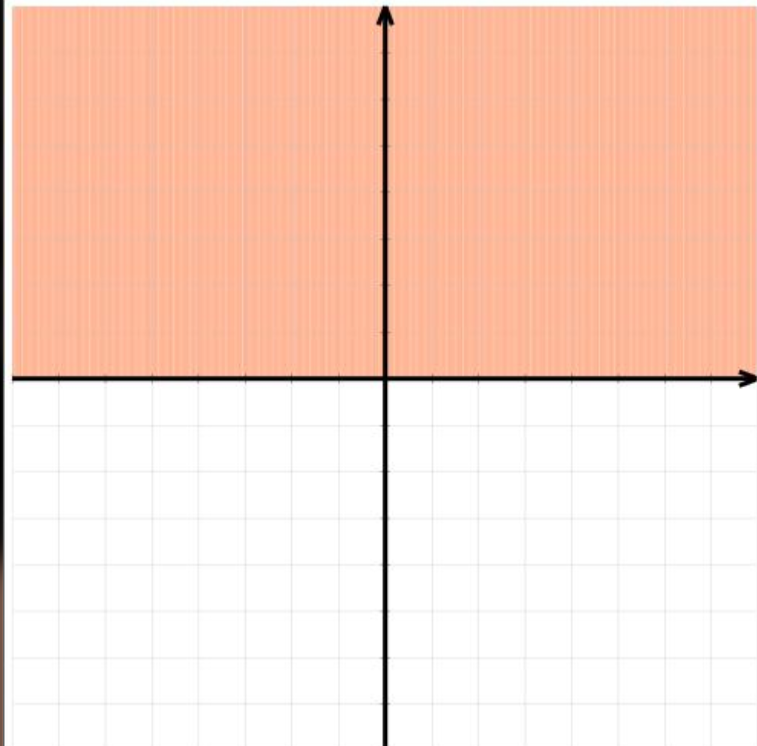
\includegraphics[width=0.4\textwidth]{_files/_images/25.png}
    \caption{Poliedro semipiano sopra l'asse \(x_1\), asse compreso.}
    \label{fig:mia_immagine}
\end{figure}

Scegliamo il punto:
\[
x=(1,2)
\]

e il vettore non nullo:
\[
d=(1,0).
\]

Variando $\lambda \in \mathbb{R}$ si hanno tutti i punti sulla retta orizzontale ad altezza $x_2 = 2$ e questi sono tutti contenuti nel Poliedro. Quindi il Poliedro contiene proprio quella retta orizzontale.

\newpage

Un importante risultato è espresso nel seguente teorema, di cui tralasciamo la dimostrazione.

\begin{theorem}{Teorema}
Sia $P=\{x\in\mathbb{R}^{n} \mid a_{i}^{\prime}x\ge b_{i}, i=1,2,...,m\}$ un poliedro non vuoto.

Le seguenti affermazioni sono equivalenti fra loro:
\begin{itemize}
    \item[(a)] $P$ ha almeno un punto estremo.
    \item[(b)] $P$ non contiene una retta.
    \item[(c)] Oltre ad $a_{1},a_{2},...,a_{m}$, esistono altri $n-m$ vettori tutti linearmente indipendenti fra loro.
\end{itemize}
\end{theorem}


Si noti che un poliedro \textbf{limitato non contiene una retta} e così anche il quadrante positivo $\{x \mid x\ge 0\}$. Dal momento che un poliedro descritto in forma standard è contenuto nel quadrante positivo, ne consegue che neanch'esso contiene una retta. Infatti, è valido il seguente corollario.

\begin{corollary}{Corollario}
Ogni poliedro limitato non vuoto ed ogni poliedro non vuoto descritto in forma standard ha almeno un punto estremo e, dunque, almeno una soluzione di base ammissibile.
\end{corollary}


\subsection{Ottimalità di punti estremi}
Come abbiamo detto anche in paragrafi precedenti, quando si parla di \textbf{soluzione ottime} per un problema di PL, si parla di queste:
\begin{figure}[htbp]
    \centering
    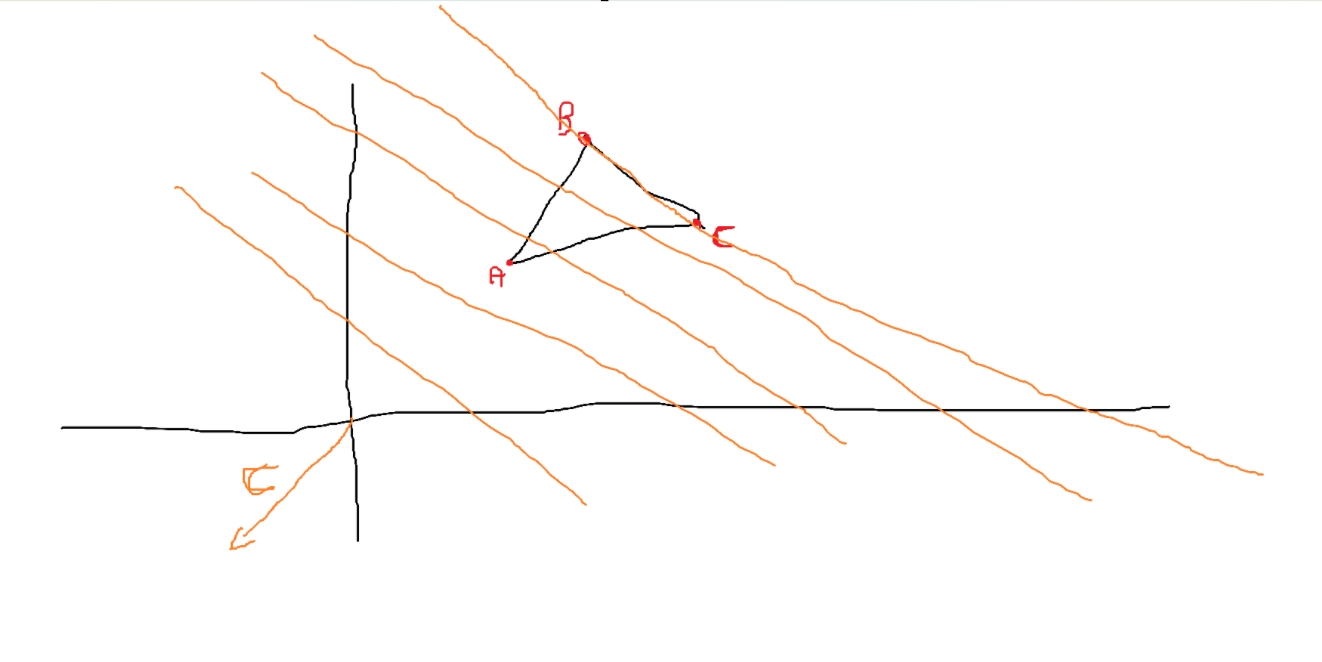
\includegraphics[width=0.4\textwidth]{_files/_images/26.png}
    \caption{Descrizione grafica di un Problema di PL, dove devo minimizzare una funzione descritta dal vettore $c$.}
    \label{fig:mia_immagine}
\end{figure}
Come vedi il vettore $c$, punta nella direzione di massima crescita, allora l'insieme di soluzioni ottime (rispettando i vincoli, quindi contenute nel poliedro, ovviamente), è tutto il segmento BC,
dove BC, sono vertici/punti di estremo/SBA.





In questo paragrafo verranno formalizzate le motivazioni per cui, come già accennato in precedenza, dato un poliedro $P$ che abbia almeno un punto estremo e che sia la regione ammissibile di un problema di PL che ammette soluzione ottima, sia sempre possibile individuare in un vertice (o, equivalentemente, in un punto estremo o soluzione ammissibile di base) di $P$ una soluzione ottima al problema stesso.

Sono validi i seguenti risultati, di cui si trascura la verifica.

\begin{theorem}{Teorema}
Si consideri il problema di PL consistente nel minimizzare $c^{\prime}x$ su un poliedro $P$ che abbia almeno un punto estremo e si supponga che il problema ammetta almeno una soluzione ottima. Allora, esiste una soluzione ottima al problema che è punto estremo di $P$.
\end{theorem}

Questo teorema si può applicare nel caso di sopra di cui vedi l'immagine.

Il risultato precedente si applica sia a poliedri in forma standard che a poliedri limitati, dato che essi non contengono una retta.


\begin{theorem}{Teorema}
Si consideri il problema di PL consistente nel minimizzare $c^{\prime}x$ su un poliedro $P$ che abbia almeno un punto estremo. Allora, o il valore della soluzione ottima è $-\infty$ oppure esiste un punto estremo di $P$ che è soluzione ottima finita del problema.
\end{theorem}

Il teorema dice che si verifica una delle seguenti due situazioni:
\begin{itemize}
    \item - Caso 1 — Problema illimitato inferiormente: il valore della funzione obiettivo può diminuire indefinitamente, fino a \(-\infty\). Non esiste un minimo finito.
    \item - Caso 2 — Ottimo finito: esiste almeno un punto estremo del poliedro che è una soluzione ottima.
\end{itemize}
La differenza rispetto al teorema precedente è che qui non devi supporre che esista già una soluzione ottima: il teorema considera anche il caso in cui il problema sia illimitato inferiormente.
2. Caso 1: problema illimitato inferiormente
Consideriamo:
\[
\begin{aligned}
\min \quad & z=-x_1\\
\text{s.t.}\quad & x_1\geq 0\\
&x_2\geq 0.
\end{aligned}
\]

Il poliedro ammissibile è il primo quadrante, che possiede un punto estremo: l'origine \(O=(0,0)\).
Tuttavia, possiamo scegliere \(x_1\) sempre più grande:
\[
\begin{array}{c|c}
x_1 & z=-x_1\\ \hline
10 & -10\\
100 & -100\\
1000 & -1000
\end{array}
\]

Il valore della funzione obiettivo diminuisce indefinitamente.
Pertanto, siamo nel Caso 1:
\[
\boxed{\inf_{x\in P}c'x=-\infty}
\]

Il teorema non garantisce un vertice ottimo finito, perché in questo caso tale vertice non esiste.
3. Caso 2: esiste un vertice ottimo finito
Consideriamo invece:
\[
\begin{aligned}
\min \quad & z=x_1+x_2\\
\text{s.t.}\quad & x_1\geq 0\\
&x_2\geq 0.
\end{aligned}
\]

Anche qui il poliedro è il primo quadrante e possiede il punto estremo \(O=(0,0)\).
Poiché entrambe le variabili sono non negative:
\[
x_1+x_2\geq 0.
\]

Il valore minimo è quindi:
\[
\boxed{z^*=0}
\]

e viene raggiunto nell'origine. L'origine è un punto estremo ed è una soluzione ottima finita.
Siamo nel Caso 2.


Nel caso di problemi di PL generici, il Teorema 2.6.7 non si applica direttamente se la regione ammissibile non ha punti estremi. Tuttavia, sappiamo che un qualunque problema di PL può essere trasformato in un problema di PL equivalente formulato in forma standard, cui il Teorema 2.6.7 invece si applica. Vale, infatti, il seguente corollario.

\begin{theorem}{Teorema}
Si consideri il problema di PL consistente nel minimizzare $c^{\prime}x$ su un poliedro $P$ non vuoto. Allora, o il valore della soluzione ottima è $-\infty$ oppure esiste una soluzione ottima finita al problema.
\end{theorem}

Questo è il teorema piu generale e non richiede manco che il Poliedro abbia vertici.

Consideriamo il problema:
\[
\begin{aligned}
\min \quad & z=x_2\\
\text{s.t.}\quad & x_2\geq 0.
\end{aligned}
\]

La variabile \(x_1\) è libera, mentre \(x_2\geq 0\).
Il poliedro ammissibile è:
\[
P=\{(x_1,x_2)\in\mathbb R^2\mid x_2\geq 0\}.
\]

È un semipiano e non possiede punti estremi: ogni suo punto appartiene a un segmento contenuto nel semipiano, quindi nessun punto è un vertice.
Eppure il problema ha una soluzione ottima finita:
\[
z^*=0.
\]

Infatti, tutti i punti della forma
\[
(x_1,0),\qquad x_1\in\mathbb R
\]

sono ammissibili e ottimi.
Questo esempio mostra perché il teorema più generale è utile: può garantire l'esistenza di una soluzione ottima finita anche quando il poliedro non ha vertici.

\section{Il Metodo del Simplesso}

Nel corso di questo paragrafo supporremo di dover risolvere il seguente generico problema di PL formulato in forma standard:
\begin{equation}
\begin{aligned}
(Pr) \quad \min \quad & c'x \
\text{s.a} \quad & Ax = b \
& x \ge 0,
\end{aligned}
\end{equation}
dove $A \in \mathbb{R}^{m \times n}$ può ha rango $m$ (il massimo, perchè $m$ < $n$). Con $A_i$ indicheremo l'i-esima colonna di $A$, mentre con $a_i'$ ne indicheremo l'i-esima riga. Supporremo, inoltre, che $P$ sia la regione ammissibile corrispondente al problema.
Supponendo sempre che $m$ < $n$.

Da quanto detto nei precedenti paragrafi è emerso che se un problema di PL formulato in forma standard ammette una soluzione ottima finita, allora esiste una soluzione ammissibile di base ottima (\textbf{i teoremi di prima}). Il metodo del simplesso si basa su tale considerazione e cerca una soluzione ottima al problema muovendosi da una soluzione ammissibile di base ad una adiacente sempre nella direzione lungo la quale si verifica un decremento del valore corrente della funzione obiettivo. Nel momento in cui viene raggiunta una soluzione ammissibile di base a partire dalla quale non è possibile intraprendere più alcuna direzione migliorativa del valore corrente della funzione obiettivo, la soluzione ammissibile di base corrente è ottima e l'algoritmo termina.

Obiettivo di questo paragrafo è analizzare il metodo del simplesso e la sua complessità computazionale, nonchè discutere di una sua particolare implementazione, nota come simplesso revisionato. Verranno anche sottolineate alcune difficoltà in cui può incorrere tale metodo in presenza di soluzioni degeneri.

\subsection{Condizioni di ottimalità}

Per risolvere un generico problema di ottimizzazione, specialmente se il problema da risolvere è NP-hard, molti algoritmi partono da una soluzione ammissibile $x$ ed esplorano soluzioni "vicine" ad $x$ (nel nostro caso, adiacenti) conservando in memoria la soluzione migliore trovata durante l'esplorazione. Tali algoritmi sono noti in letteratura come algoritmi di ricerca locale e producono in output una soluzione ottima localmente alla soluzione ammissibile iniziale $x$.

Sfortunatamente, in generale una soluzione ottima localmente non è necessariamente ottima globalmente. Il metodo del simplesso, passando da una soluzione ammissibile di base ad una soluzione ammissibile di base adiacente e terminando quando non esiste una soluzione ammissibile di base migliore, può essere interpretato come algoritmo di ricerca locale. Fortunatamente, però, nel caso di problemi di PL, dal momento che si tratta di ottimizzare una funzione obiettivo convessa su una regione ammissibile convessa, si è certi che l'ottimo locale restituito in output dal metodo del simplesso è ottimo anche globalmente. Ma come è possibile individuare una direzione lungo la quale si verifica un decremento del valore corrente della funzione obiettivo a partire dalla soluzione ammissibile di base corrente? In altri termini, data la soluzione ammissibile di base corrente $x \in P$ a partire dalla quale vogliamo muoverci lungo la direzione di un certo vettore $d \in \mathbb{R}^n$, come va scelto detto vettore $d$?

Innanzitutto, dobbiamo limitare la scelta di $d$ a quei vettori che non ci conducano fuori dalla regione ammissibile $P$. Tale osservazione porta immediatamente alla seguente definizione:

\begin{definition}{Direzione ammissibile}
Sia $x \in P \subset \mathbb{R}^n$. Un vettore $d \in \mathbb{R}^n$ è detto direzione ammissibile a partire da $x$ se esiste uno scalare $\theta > 0$ tale che $x + \theta d \in P$.
\end{definition}

\subsubsection{L'Idea del Simplesso per Costruire la Direzione $d$}
Sia $x$ una soluzione ammissibile di base per il problema formulato in forma standard (Pr).Per il teorema \ref{teorema SBA} per una SBA esistono $B(1), B(2), \dots, B(m)$ gli indici delle variabili di base e $B = [A_{B(1)} \ A_{B(2)} \ \dots \ A_{B(m)}]$ la corrispondente matrice di base. Sappiamo che $x_B = (x_{B(1)} \ x_{B(2)} \ \dots \ x_{B(m)})^T = B^{-1}b$, mentre tutte le variabili non di base sono nulle, cioè $x_N = 0$.

Quindi sempre per il teorema \ref{teorema SBA} in una Soluzione Ammissibile di Base (SAB) $x$:
\begin{itemize}
    \item $m$ variabili sono di base ($x_B$) e possono assumere valori maggiori o uguali a zero ($x_B = B^{-1}b \ge 0$).
    \item $n - m$ variabili sono non di base ($x_N$) e valgono esattamente $0$
\end{itemize}

Per muoverci verso un nuovo punto ammissibile (nel poliedro), l'algoritmo fa entrare in base una sola variabile fuori base $x_j$, lasciando le altre $n - m - 1$ variabili fuori base ferme a $0$: 

\begin{enumerate}
    \item Per la variabile entrante $x_j$: Poniamo la sua direzione $d_j = 1$, così il suo valore passa da $0$ a $\theta \cdot 1 = \theta > 0$.
    \item Per le altre variabili fuori base $x_i$ ($i \neq j$): Poniamo $d_i = 0$, quindi rimangono fisse a $0$.  
    \item Per le variabili di base $x_B$: Il vettore delle variabili di base si modifica di $\theta d_B$ per compensare la crescita di $x_j$ e garantire che i vincoli rimangano soddisfatti ($A(x + \theta d) = b$).
\end{enumerate}
Quindi quando si fanno entrare le variabili fuori base, dobbiamo anche aggiustare le variabili della base, per rispettare i vincoli, faccio un esempio cosi si chiarisce:\\
Ipotizziamo di avere un singolo vincolo:$$x_1 + 2 x_2 = 10$$Stato iniziale:$x_1$ è in base, $x_2$ è fuori base ($x_2 = 0$).Quindi $x_1 = 10$. Il vincolo è soddisfatto: $10 + 2(0) = 10$.Ora vogliamo far crescere $x_2$ di una quantità $\theta = 3$:La variabile $x_2$ passa da $0$ a $3$.Cosa succederebbe se $x_1$ NON cambiasse valore?$$10 + 2(3) = 16 \neq 10 \quad \text{(Vincolo violato!)}$$Per "compensare" l'aggiunta di $+6$ data da $2 x_2$, la variabile di base $x_1$ deve ridursi di $6$, passando da $10$ a $4$:$$4 + 2(3) = 10 \quad \text{(Vincolo di nuovo soddisfatto!)}$$
\textbf{Questo perchè noi vogliamo sempre rimanere nei vincoli del Poliedro definito dal problema}
\begin{center}
    Nel procedimento seguente quello che facciamo è ricavarci $d_B$ assumendo che $d$ già esista.
\end{center}

\begin{observation}{Osservazione}
    $d$ è un vettore, e come tale ha i suoi componenti. Ricordati che con $x_B$ è un vettor e  indichiamo i componenti base di $x$, questi sono tipo:
    \begin{center}
        $x_1,x_2,x_4,...$
    \end{center}
    Questi contiene anche indici "sparpagliati".
    Con $d_B$ si andranno a indicare i componenti che si andranno a sommare a quelli di $x$, quindi avranno gli stessi indici, ad esempio se $x_B = [x_1,x_4]^T$ allora $d_B = [d_1,d_4]^T$
\end{observation}

Quindi formalizzando il tutto:
Innanzitutto, muovendoci da $x$ a $x + \theta d$ noi vogliamo comunque rimanere all'interno della regione ammissibile $P$:
\begin{equation}
A(x + \theta d) = b
\end{equation}
Intanto, $Ax = b$ dato che $x$ è ammissibile, per cui la relazione è equivalente a richiedere che $A \theta d = 0 \Rightarrow Ad = 0$. Dunque,
\[
0 = Ad = \sum_{i = 1}^{m} A_{B(i)} \footnote{l'indice $i$ scorre semplicemente da $1$ ad $m$ per contare le $m$ componenti della base, ma le posizioni $B(i)$ all'interno della matrice $A$ possono essere sparse in qualsiasi punto} * d_{B(i)} + \sum_{l != B(1)...B(m)} A_l d_l
\]
Questo perchè la colonna ad esempio $A_1$ usa solo il primo elemento di $d$ ecc... \\
Ricordando che $d_j = 1$ e $d_i = 0$ per ogni $i \neq j, \text{ e } i \neq B(1), B(2), \dots, B(m)$, si ottiene:
\begin{equation}
B d_B + A_j.
\end{equation}
Dal momento che la matrice $B$ è invertibile, è possibile concludere che:
\begin{equation}
d_B = -B^{-1} A_j
\end{equation}
Il vettore $d$ appena costruito è noto come \textbf{j-esima direzione di base}.
Il vettore d appena costruito `e noto come j.ma direzione di base. Esso
garantisce il rispetto dei vincoli di uguaglianza che descrivono la regione ammissibile P, ma cosa possiamo dire del rispetto dei vincoli di non negatività
delle variabili di decisione $x + \theta d $ >= 0?
Con l'introduzione di d sicuramente il valore della variabile non di base
$x_j$ è passato da 0 a $\theta$ > 0, mentre il valore delle restanti $n-m-1$ variabili non
di base è rimasto nullo. Dunque, nel rispondere alla domanda precedente,
dobbiamo preoccuparci solo del nuovo valore delle variabili di base e cioè di
$x_B + \theta d_B$ e distinguiamo due casi:
\begin{itemize}
\item[(a)] $x$ è una soluzione ammissibile di base \textbf{non degenere}. Ciò implica che $x_B > 0$.

\paragraph{Motivazione:}
Per definizione, una soluzione di base è \textbf{non degenere} se attiva \textbf{esattamente $n$ vincoli} linearmente indipendenti.

Nel modello in forma standard ($Ax = b, \, x \ge 0$ con $m < n$ e $\text{rank}(A) = m$), la costruzione di una soluzione di base prevede di selezionare una matrice di base $B$ formata da $m$ colonne linearmente indipendenti di $A$, ponendo a zero le restanti $n - m$ variabili fuori base ($x_N = 0$).

Ciò attiva già esattamente $n$ vincoli:
\begin{itemize}
    \item gli $m$ vincoli di uguaglianza strutturali ($Ax = b$) (\textbf{grazie anche alle variabili messe a 0, altrimenti non li attiverebbe}), quindi le variabili fuori base \(x_N\) vengono fissate a zero e le variabili di base \(x_B\) assumono i valori necessari per soddisfare gli \(m\) vincoli.
    \item gli $n - m$ vincoli di non-negatività per le variabili fuori base ($x_N = 0$), per raggiungere gli $n$ vincoli.
\end{itemize}

Se una qualsiasi variabile di base fosse nulla ($x_{B(i)} = 0$), si otterrebbe l'attivazione di un $(n+1)$-esimo vincolo di non-negatività. Poiché per la non-degenerazione i vincoli attivi devono essere esattamente $n$, nessuna variabile di base può valere zero. Trattandosi di una soluzione ammissibile ($x \ge 0$), deve quindi valere strettamente $x_B > 0$.

Per cui in questo caso:
\begin{enumerate}
    \item \textbf{$x_B$} è > 0
    \item $\theta$ > 0
    \item L'unico che può essere positivo o negativo è $d_B$ (\textbf{o meglio le sue componenti del vettore possono essere positive o negative}):
    \begin{itemize}
        \item \textbf{$d_{B(i)} >= 0$} : La variabile di base $x_{B(i)}$ aumenta (o rimane costante) man mano che si aumenta $\theta$:$$x_{B(i)} + \theta d_{B(i)} \ge x_{B(i)} > 0$$
        \item \textbf{$d_{B(i)} < 0$} : La variabile di base $x_{B(i)}$ diminuisce man mano che si aumenta $\theta$:$$x_{B(i)} + \theta d_{B(i)}$$   
    \end{itemize}
\end{enumerate}

per cui per $\theta$ sufficientemente piccolo, la non negatività è preservata e $d$ è una direzione ammissibile.
\item[(b)] $x$ è una soluzione ammissibile di base \textbf{degenere}. In questo caso, può accadere che una variabile di base $x_{B(i)}$ sia nulla, mentre la corrispondente componente $d_{B(i)}$ sia negativa. In tale ipotesi, se seguissimo la direzione $d$ abbandoneremmo la regione ammissibile $P$.
Questo perchè ci troveremo delle variabili negative che violano i vincoli del problema.
\end{itemize}


\begin{center}
    La direzione in cui ci ritroviamo con il nuovo punto, non sarà un punto casuale, ma sarà un punto che si trova adiacente a $x$, sulla sua frontierà, questo perchè per scegliere la direzione $d$, fai entrare in base una sola variabile fuori base alla volta.
    questo equivale a disattivare esattamente 1 vincolo di non-negatività, invece di avere $n$ vincoli attivi (che identificano un singolo punto $0$-dimensionale, il vertice), ti ritrovi con $n - 1$ vincoli attivi.
    La nuova soluzione avrà proprio la definizione di adiacenza, questo perchè soddisfa gli $m$ vincoli originali (imposti nell'equazione \textbf{3.51}) e i restanti $n-m-1$ di non negatività, quindi in totale $n-1$ vincoli, quindi sarà adiacente a $x$.
\end{center}


Supponiamo di aver individuato una direzione ammissibile $d$, e di essere pronti a spostarci da $x$ a $x + \theta d$.
è chiaro che effettueremo effettivamente lo spostamento solo qualora esso fosse conveniente in termini di decremento del valore della funzione obiettivo, che ora sarà
\begin{equation}
c'(x + \theta d) = c'x + \theta c' d
\end{equation}
Valutiamo dunque $c'd$. Ricordando che per ipotesi le componenti $d_i = 0$ per ogni $i \neq j,B(1),\dots,B(m)$ e $d_j = 1$, si ha che:
\begin{equation}
    c'd = c'_B d_B + c_j =^{def} -B^{-1} A_j c'_B + c_j = c_j -B^{-1} A_j c'_B
\end{equation}
Portando a sinistra il termine si ha:
$$\Delta \text{Costo} = c'(x + \theta d) - c'x = \theta \cdot (c'd)$$.
La variazione di costo rappresenta quanto cambia il valore della funzione obiettivo quando ci spostiamo dalla soluzione corrente \(x\) a una nuova soluzione \(x+\theta d\).
\paragraph{Esempio intuitivo}
Supponiamo di voler minimizzare il costo di produzione di due prodotti.
\begin{enumerate}
    \item Situazione iniziale: costo pari a \(100\,€\).
    \item Dopo uno spostamento lungo una direzione \(d\): costo pari a \(80\,€\).
\end{enumerate}
La variazione di costo è:
\[
\Delta Costo=80-100=-20\,€
\]

Il costo è diminuito di \(20\,€\), quindi lo spostamento è migliorativo.

Questo spiega immediatamente il comportamento del sistema:
\begin{itemize}
    \item $c'd < 0$: Il tasso di variazione è negativo, quindi la funzione decresce (la direzione è di discesa).
    \item $c'd > 0$: Il tasso di variazione è positivo, quindi la funzione cresce (la direzione è di salita).
    \item $c'd = 0$: Il tasso di variazione è nullo, quindi ti muovi lungo una linea di livello in cui il costo non varia
\end{itemize}

\[
\underbrace{\theta}_{\text{quanto ci spostiamo}}
\cdot
\underbrace{(c'd)}_{\text{variazione per unità di }\theta}
=
\underbrace{\Delta Costo}_{\text{variazione totale}}
\]

\begin{observation}{Derivata direzionale}
La derivata (base, parziale e direzionale) misura il tasso di variazione istantaneo della funzione in un punto, indicando se essa sta crescendo, decrescendo o rimanendo stazionaria.Dal punto di vista geometrico, se la derivata parziale analizza la funzione restringendosi lungo l'asse di una coordinata, la derivata direzionale generalizza questo concetto sezionando il grafico della funzione con un piano verticale parallelo a una generica direzione $d$. Tale intersezione genera una curva unidimensionale, e la derivata direzionale rappresenta la pendenza (il coefficiente angolare della retta tangente) a questa curva nel punto considerato.Per una funzione lineare $f(x) = c'x$ (con $c, x \in \mathbb{R}^n$), il gradiente è costante in tutto il dominio:$$\nabla f(x) = c \quad \forall x \in \mathbb{R}^n$$Per ogni funzione differenziabile, la derivata direzionale nel punto $x_0$ lungo la direzione $d$ è espressa dal prodotto scalare:$$D_d f(x_0) = \nabla f(x_0)' d = c'd$$
Ad esempio, consideriamo una determinata direzione individuata da un vettore unitario. Se la derivata direzionale della funzione in un punto, lungo quella direzione, è pari a \(5\), significa che la funzione sta aumentando, in quel punto e lungo quella direzione, con una pendenza pari a \(5\). 
La derivata direzionale lungo la direzione \(d\) è \(c'd\). Questo valore rappresenta la variazione della funzione per unità di spostamento lungo tale direzione. Se ci spostiamo, a partire dal punto iniziale, di \(\theta d\), significa che percorriamo \(\theta\) volte la direzione \(d\). Di conseguenza, **la variazione della funzione, assumendo che la funzione sia lineare, è pari a**
\[
\theta c'd.
\]
\end{observation}


\begin{definition}{Costo ridotto}
Sia $x$ una soluzione di base, $B$ la matrice di base ad essa corrispondente e sia $c_B$ il vettore dei costi associati alle variabili di base. Per ogni $j$, si definisce costo ridotto $\bar{c}_j$ della variabile $x_j$ la seguente quantità:


$$\bar{c}_j = c_j - c_B' B^{-1} A_j$$


è uno scalare.
\textbf{Teoricamente si può calcolare per qualsiasi variabile di base e non.}
\end{definition}
\paragraph{Esempio per capire cosa sono i costi ridotti di una variabile $x_j$}
Supponiamo di voler minimizzare:
\[
\min z=3x_1+5x_2+4x_3
\]

soggetto ai vincoli:
\[
\begin{cases}
x_1+x_2+x_3=4\\
x_1,x_2,x_3\geq 0
\end{cases}
\]

I costi delle variabili sono:
\[
c_1=3,\qquad c_2=5,\qquad c_3=4
\]
Supponiamo di considerare la soluzione di base:
\[
x=(4,0,0)
\]

In questo caso, \(x_1\) è la variabile di base, mentre \(x_2\) e \(x_3\) sono variabili non di base.
La matrice di base è semplicemente:
\[
B=[1]
\]

e il vettore dei costi delle variabili di base è:
\[
c_B=[3]
\]
\[
\begin{aligned}
\bar c_2
&=5-[3][1][1]\\
&=5-3\\
&=\boxed{2}
\end{aligned}
\]

Il costo ridotto di \(x_2\) è quindi \(2\).
Ma cosa significa?
Attualmente abbiamo:
\[
x=(4,0,0),\qquad z=3\cdot4=12
\]
Ora immaginiamo di aumentare \(x_2\) da \(0\) a \(1\).Quindi $\theta = 1$
Otteniamo quindi:
\[
x=(3,1,0)
\]
\textbf{Vengono cambiate tramite $dB$ anche le variabile di base, per rispettare i vincoli}.
Calcoliamo il nuovo costo della funzione obiettivo:
\[
z=3\cdot3+5\cdot1=14
\]
Il costo è passato da 12 a 14.
Ritorniamo al costo ridotto che abbiamo calcolato prima:
\[
\bar c_2=5-3=2
\]
\begin{enumerate}
    \item Inserire un'unità (1 proprio, perchè prima $x_2$ era 0) di \(x_2\) costa \(5\) (perchè nella funzione di costo vi è $5x_2$).
    \item Per farle spazio, togliamo un'unità di \(x_1\), risparmiando \(3\) (perchè nella funzione di costo vi è $3x_1$)
    \item La variazione netta del costo è \(5-3=2\) per quelle due variabili (di base e non) nella funzione di costo. Quindi introdurre \textbf{un'unita di $x_2$} (tramite $\theta = 1$), non fa diminuire il costo della funzione, perchè aggiungere $x_2$ (un'unità) mi costa troppo anche levando $x_1$, e quindi \textbf{aggiungere un'unita di $x_2$ mi costa 2}, e quindi la funzione obiettivo aumenta di 2, rispetto alla soluzione iniziale.
\end{enumerate}
Quindi il costo ridotto di una variabile mi indica proprio questo, però \textbf{in modo unitario}, cioè aggiungendo una copia di $x_2$ alla base, quanto varia il costo della funzione sul nuovo punto, rispetto alla soluzione originale.
Di solito però non aggiungo una copia, ma ne aggiungo in generale $\theta$, quindi per calcolare la variazione totale della funzione di costo moltiplico il costo unitario ($c^-_j$) per quante copie aggiungo ($\theta$)
,io in questo caso ho scelto $\theta = 1$ per semplicità perciò la variazione di $z$ e il costo ridotto combaciavano, ma in generale:
\[
\Delta z = z(x+\theta d) - z(x) = \theta \bar{c}_j
\]
Quindi il costo ridotto rispetto ad una variabile $j$ mi indica quanto costa aggiungere quella variabile alla base, (tenendo conto che sono cambiate anche le variabili di base grazie a $d_B$),in modo unitario cioè aggiungendo solo una copia.
\\
In generale, per un problema di minimizzazione, se consideriamo una variabile non di base:
\begin{itemize}
    \item \(\bar c_j<0\): muoversi in quella direzione (cioè nella direzione $d$ che viene fuori introducendo $x_j$) fa diminuire la funzione obiettivo (buono per problemi di minimizzazione).
    $\theta$ indica quanto mi muovo in quella direzione, e se muoversi in quella direzione fa diminuire la funzione, dato che la funzione è lineare, è bene continuare ad aumentare la direzione in quella funzione.

    \item \(\bar c_j=0\): muoversi in quella direzione lascia invariato il valore della funzione obiettivo.

    \item \(\bar c_j>0\): muoversi in quella direzione fa aumentare la funzione obiettivo (peggioramento per problemi di minimizzazione).
\end{itemize}


\begin{example}{Calcolo della direzione di base e del costo ridotto}
Si consideri il seguente problema di PL:
\begin{align*}
\min \quad & c_1 x_1 + c_2 x_2 + c_3 x_3 + c_4 x_4 \
\text{s.a} \quad & x_1 + x_2 + x_3 + x_4 = 2 \
& 2x_1 + 3x_3 + 4x_4 = 2 \
& x \ge 0
\end{align*}
Le prime due colonne della matrice $A$, $A_1 = [1 \ 2]^T$ e $A_2 = [1 \ 0]^T$, sono linearmente indipendenti, per cui possiamo scegliere $x_1$ e $x_2$ come variabili di base:


$$B = \begin{bmatrix} 1 & 1 \\ 2 & 0 \end{bmatrix}$$


Annulliamo le variabili non di base $x_3 = x_4 = 0$ e calcoliamo $x_B = B^{-1}b$, ottenendo $x_1 = x_2 = 1$. Dunque $x = (1, 1, 0, 0)$ è una soluzione ammissibile di base non degenere. Una direzione di base $d$ (facendo entrare $x_3$) avrà $d_3 = 1, d_4 = 0$ e:


$$d_B = \begin{pmatrix} d_1 \\ d_2 \end{pmatrix} = -B^{-1} A_3 = -\begin{bmatrix} 0 & 1/2 \\ 1 & -1/2 \end{bmatrix} \begin{bmatrix} 1 \\ 3 \end{bmatrix} = \begin{bmatrix} -3/2 \\ 1/2 \end{bmatrix}$$


Il costo per muoversi lungo $d$ è pari a $c'd = -\frac{3}{2}c_1 + \frac{1}{2}c_2 + c_3 = \bar{c}_3$.
\end{example}

Si noti che per ogni variabile di base $x_{B(i)}$, il suo costo ridotto è nullo:


$$\bar{c}_{B(i)} = c_{B(i)} - c_B' B^{-1} A_{B(i)} = c_{B(i)} - c_B' e_i = c_{B(i)} - c_{B(i)} = 0$$

\begin{theorem}{Condizioni di ottimalità}
Sia $x$ una soluzione ammissibile di base, $B$ la matrice di base ad essa associata e sia $\bar{c}$ il corrispondente vettore dei costi ridotti.
\begin{itemize}
    \item[(a)] Se $\bar{c} \ge 0$, allora $x$ è ottima.
    \item[(b)] Se $x$ è ottima e non degenere, allora $\bar{c} \ge 0$.
\end{itemize}
\end{theorem}

\paragraph{Interpretazione delle condizioni di ottimalità.}

Se tutti i costi ridotti sono non negativi, nessuna variabile non di base può essere incrementata, lungo la corrispondente direzione elementare del simplesso, per ridurre il valore della funzione obiettivo. Di conseguenza, la soluzione di base ammissibile corrente è ottima.

Questo perché, una volta calcolato il vettore dei costi ridotti, abbiamo una panoramica delle variazioni della funzione obiettivo associate alle direzioni elementari del simplesso, ciascuna corrispondente all'introduzione di una variabile non di base.

Ad esempio, per valutare l'introduzione della variabile non di base $x_3$, costruiamo una direzione $d$ in cui la componente associata a $x_3$ è posta uguale a $1$, mentre le altre componenti associate alle variabili non di base sono poste uguali a $0$. Le componenti $d_B$ relative alle variabili di base vengono determinate in modo da mantenere soddisfatti i vincoli di uguaglianza:

Ripetiamo questo procedimento per ogni variabile non di base, ottenendo le rispettive direzioni elementari.

Quindi ad esempio, se:
\[
\bar{c}=(0,0,2,5),
\]
e $x_3$ e $x_4$ sono le variabili non di base, abbiamo:
\[
\bar{c}_3=2, \qquad \bar{c}_4=5.
\]

Questo significa che, lungo la direzione elementare associata a $x_3$, ogni incremento di $\theta$ determina un aumento della funzione obiettivo pari a $2\theta$. Analogamente, introducendo $x_4$, la funzione obiettivo aumenta di $5\theta$.

Pertanto, se tutti i costi ridotti sono non negativi, nessuna delle direzioni elementari del simplesso permette di migliorare la soluzione corrente. Per il teorema delle condizioni di ottimalità, la soluzione di base ammissibile corrente è quindi ottima.


\paragraph{Nota} : Nella nuova direzione che considero, c'è anche $\theta$, cioè:
\[
x + \theta d
\]
ma $\theta$ non cambia la direzione, indica solo QUANTO mi sposto in quella direzione, se il vettore dei costi è tutto positivo (come prima) dato che $\theta \ge 0 $, i costi "possono" solo peggiorare.

\subsection{Il Metodo del Simplesso}

Supponiamo di trattare soluzioni ammissibili di base non degeneri. Se esiste un costo ridotto $\bar{c}_j < 0$, allora la j-esima direzione di base $d$ porta ad un decremento del valore della funzione obiettivo
\textbf{Ora devo capire però quanto spostarmi, in quella direzione, tramite il parametro $\theta$.
Io ho trovato la direzione in cui spostarmi, introducendo la variabile non di base nella base, e visualizzando il costo ridotto di quella variabile, ma ora devo capire quanto spostarmi, per rimanere ancora ammissibile, perchè potrei uscire fuori dai bordi}
Infatti guarda:

Supponiamo di avere una soluzione di base ammissibile \(x\) e di individuare una variabile non di base \(x_j\) con costo ridotto negativo:
\[
\bar c_j<0
\]

Questo significa che, lungo la direzione di base \(d\) associata all'introduzione di \(x_j\), la variazione della funzione obiettivo è:
\[
\Delta z=\theta\bar c_j
\]

Dato che \(\theta>0\) e \(\bar c_j<0\), la funzione obiettivo diminuisce.
Quindi abbiamo individuato una direzione di miglioramento. Ma non sappiamo ancora quanto possiamo percorrerla restando ammissibili ($aumentare \theta$).
\\
Vogliamo quindi raggiungere il punto che massimizza tale decremento rimanendo ammissibili:


$$\theta^* = \max \{ \theta > 0 \mid x + \theta d \in P \}$$

Questo perchè dato che la funzione è lineare, una volta scelto la direzione $d$, se questa è peggiorativa, io posso seguirla, sapendo che il valore della funzione obiettivo continua a peggiorare.
Ovviamente però posso seguirla solo fino ad un certo punto, altrimenti esco fuori dalla regione ammissibile.

\paragraph{Come calcolo \(\theta^*\)?}
Nel simplesso in forma standard, le variabili devono essere non negative. Le variabili non di base partono da zero e, nella direzione associata all'ingresso di \(x_j\), quella variabile aumenta.
Le variabili di base, invece, cambiano secondo le componenti \(d_B\) della direzione. Per ogni variabile di base \(x_{B(i)}\), dobbiamo rispettare:
\[
x_{B(i)}+\theta d_{B(i)}\geq 0
\]
Ora distinguiamo due casi.
\begin{enumerate}
    \item \textbf{Caso 1: tutte le componenti di $d_B$ sono non negative} : 
    Se \(d_B\geq 0\), le variabili di base non diminuiscono: aumentano oppure rimangono invariate. Anche la variabile non di base entrante aumenta.
    Di conseguenza, non incontriamo un limite dovuto ai vincoli di non negatività e possiamo aumentare \(\theta\) indefinitamente:
    \[
    \theta^*=+\infty
    \]
    Se il costo ridotto della variabile entrante è negativo, la funzione obiettivo continua a diminuire indefinitamente. Il problema è quindi illimitato inferiormente.
    \textbf{Nota: Io posso aumentare $\theta$ a piacere basta che sia maggiore di 0, senza preoccuparmi del se vengono rispettati i vincoli del sè} $x+\theta d$ è una soluzione di base ammissibile,
    questo perchè abbiamo già visto nella dimostrazione di prima, che questo dipende solo da $Ad = 0$, l'unica cosa da vedere è l'ammissilibtà, cioè che tutti gli elementi siano >=0, ma nel caso 1 è soddisfatto perchè le componenti di $d_B$ sono positive, $x$ è non negativo e $\theta$ è maggiore di 0
    \item \textbf{Caso 2 : almeno una componente di $d_B$ è negativa} : 
    Se \(d_{B(i)}<0\), la corrispondente variabile di base diminuisce quando aumentiamo \(\theta\).
    Per mantenere la sua non negatività:
    \[
    x_{B(i)}+\theta d_{B(i)}\geq 0
    \]

    Isolando \(\theta\), otteniamo:
    \[
    \theta\leq-\frac{x_{B(i)}}{d_{B(i)}}
    \]

    Ogni variabile di base che diminuisce impone quindi un limite massimo allo spostamento. \textbf{Per non violare nessuno dei vincoli, scegliamo il limite più piccolo}:
    \[
    \boxed{
    \theta^*=
    \min_{\substack{i=1,\ldots,m\\d_{B(i)}<0}}
    \left\{-\frac{x_{B(i)}}{d_{B(i)}}\right\}
    }
    \]
\end{enumerate}
\paragraph{Esempio}
Supponiamo che le variabili di base siano inizialmente:
\[
x_B=\begin{pmatrix}6\\4\end{pmatrix}
\]

e che, lungo la direzione scelta, cambino secondo:
\[
d_B=\begin{pmatrix}-2\\-1\end{pmatrix}
\]

Le nuove variabili di base sono:
\[
x_B(\theta)=
\begin{pmatrix}
6-2\theta\\
4-\theta
\end{pmatrix}
\]

Calcoliamo i limiti imposti dalle due variabili:
\(6-2\theta\geq0\) \text{ quindi }	\(\theta\leq3\) \text{ e }
\(4-\theta\geq0\) \text{ quindi }	\(\theta\leq4\)
Quindi:
\[
\theta^*=\min\{3,4\}=3
\]
\textbf{$\theta$ indica lo spostamento massimo che io posso fare in quella direzione, mantenendo i vincoli}.

Alla fine dello spostamento:
\[
x_B(3)=
\begin{pmatrix}0\\1\end{pmatrix}
\]

La prima variabile di base raggiunge zero, quindi esce dalla base, mentre la variabile non di base che avevamo scelto inizialmente entra nella base.

nel simplesso, quando effettuiamo il massimo spostamento ammissibile, almeno una variabile di base raggiunge zero cioè quella con vincolo minimo. Se più variabili raggiungono zero contemporaneamente, possiamo avere una situazione di degenerazione.

Quindi ricapitolando:

\begin{enumerate}
    \item Condizione di Soluzione di Base (in $\mathbb{R}^n$):Un punto è una soluzione di base se sono attivi (ossia soddisfatti con il segno di uguaglianza) $n$ vincoli linearmente indipendenti:Gli $m$ vincoli di uguaglianza $Ax = b$.   $n - m$ vincoli di non-negatività $x_j = 0$ corrispondenti alle variabili non in base.
    \item \textbf{Cosa succede durante lo spostamento nel simplesso:}
    \begin{itemize}
        \item  Inizio ($x$): Sulla soluzione corrente sono attivi $n$ vincoli ($m$ di uguaglianza e $n-m$ di non-negatività).
        \item  Spostamento ($\theta > 0$): Scegliendo di far entrare in base una variabile $x_j$, rilasci il suo vincolo di non-negatività ($x_j$ diventa $>0$).  In questa fase ti stai muovendo lungo uno spigolo del poliedro e hai temporaneamente $n-1$ vincoli attivi
        \item  Arrivo ($\theta = \theta^*$): Scegliendo il passo massimo ammissibile $\theta^* = \min \left\{ -\frac{x_{B(i)}}{d_{B(i)}} \right\}$, la prima variabile di base $x_{B(l)}$ che tocca zero attiva un nuovo vincolo di non-negatività ($x_{B(l)} = 0$)
    \end{itemize}
    \item Conteggio finale dei vincoli attivi in $x + \theta d$: 
    \begin{itemize}
        \item  $m$ vincoli di uguaglianza $A (x + \theta d) = b$. Questo perchè per la questione che abbiamo detto prima deve essere solo soddisfatto $Ad = 0$   
        \item $n - m - 1$ vincoli di non-negatività delle variabili rimaste fuori base.
        \item $1$ nuovo vincolo di non-negatività $x_{B(l)} = 0$ della variabile uscita dalla base.
    \end{itemize}
\end{enumerate}
Quindi sostanzialmente si passa da una SBA ad un'altra, difatti durante un'iterazione del simplesso, il movimento da $x$ al nuovo punto $\bar{x} = x + \theta^* d$ corrisponde geometricamente a camminare lungo uno spigolo del poliedro per passare da un vertice al vertice adiacente che migliora (o non peggiora) il valore della funzione obiettivo. 
L'algoritmo del simplesso non fa altro che esplorare la superficie del poliedro muovendosi di vertice in vertice lungo i bordi, finché non trova un vertice in cui nessuna direzione di movimento porta ad un miglioramento (l'ottimo).

\begin{theorem}{Sostituzione della base}
Consideriamo $l$ sia l'indice della variabile che è appena uscita dalla base (perchè diventata 0)
Valgono le seguenti proprietà:
\begin{itemize}
\item[(a)] Le colonne $A_{B(i)}$, $i \neq l$, e $A_j$ ($j$ è l'indice della variabile che è entrata in base) sono linearmente indipendenti e la nuova matrice $\bar{B}$ è una base;
\item[(b)] Il punto $\bar{x} = x + \theta^* d$ è una soluzione di base ammissibile associata alla matrice di base $\bar{B}$.
\end{itemize}
\end{theorem}

Ecco i passi formali di una iterazione del simplesso:
\begin{enumerate}
\item Sia $B = [A_{B(1)} \dots A_{B(m)}]$ una matrice di base associata alla soluzione ammissibile $x$.
\item Calcolare il costo ridotto $\bar{c}_j = c_j - c_B' B^{-1} A_j$ per le variabili non di base. Se $\bar{c}_j \ge 0$ per ogni $j$, l'algoritmo termina ($x$ è ottima). Altrimenti, scegliere un $j$ con $\bar{c}_j < 0$.
\item Calcolare $u = B^{-1} A_j$ $u = -d_B$. Se $u \le 0$, allora $\theta^* = \infty$ e il costo ottimo è $-\infty$.
\item Calcolare $\theta^* = \min_{\{i \mid u_i > 0\}} \left\{ \frac{x_{B(i)}}{u_i} \right\}$.
\item Sia $l$ l'indice per cui si realizza il minimo. Rimpiazzare $A_{B(l)}$ con $A_j$ per formare $\bar{B}$ e aggiornare la soluzione.
\end{enumerate}
Il metodo del simplesso è inizializzato con una qualunque soluzione di base
ammissibile, che è garantita esistere per problemi ammissibili in forma standard.
E l'algoritmo si ferma quando trova una soluzione di base ammissibile ottima, cioè dove i costi ridotti assocciati alla variabile sono tutti >= 0, questo significa che muovendosi non c'è miglioramento da nessuna parte.


\newpage

\begin{theorem}{Terminazione del Simplesso}
Sia dato un problema di PL avente regione ammissibile $P$ non vuota. Supponiamo che ogni soluzione ammissibile al problema sia \textbf{non degenere}, allora il metodo del simplesso termina dopo un numero finito di iterazioni.
Ricorda che : \\ 
Una soluzione di base ammissibile è non degenere se tutte le sue \(m\) variabili di base sono strettamente positive:
\[
\boxed{x_{B_i}>0 \quad \forall i=1,\ldots,m}
\]
\end{theorem}

\subsection{Il Metodo del Simplesso per problemi degeneri: regole di pivoting}
Supponiamo di applicare il metodo del simplesso per risolvere un problema
di PL che ammetta qualche soluzione ammissibile di base degenere. Allora,
nel corso dell'algoritmo possono verificarsi i seguenti due casi.
\begin{enumerate}
    \item La soluzione ammissibile di base corrente $x$ è \textbf{degenere}. In questo caso,
$\theta^*$ può risultare nullo e di fatto la nuova soluzione $\hat{x}$ coinciderebbe
con x stessa (due basi differenti cui corrisponde la stessa soluzione di
base).

Questo perchè se $x$ è degenere, significa che una sua variabile di base è uguale a 0, quindi quando si fa il test
\[
    \boxed{
    \theta^*=
    \min_{\substack{i=1,\ldots,m\\d_{B(i)}<0}}
    \left\{-\frac{x_{B(i)}}{d_{B(i)}}\right\}
    }
\]
per scegliere $\theta$ cioè l'ampiezza in cui devo muovermi, questo è 0, cioè $\theta = 0$, questo perchè il minimo è uguale a 0, e non ci può essere nessuno di piu piccolo.
Quindi $x + \theta d$, $d = 0$ $\implies$ $x$.
Quindi si annulla completamente la direzione $d$ che avevamo scelto per spostarci.
\textbf{A livello di matrice di base però, la struttura cambia}. Una variabile esce dalla base (con indice $j$ relativa alla direzione $d$) e la variabile entrante vi subentra (assumendo valore pari a $0$, che è proprio quella variabile di base che aveva già valore pari a zero, ovviamente però il cambiamento non avviene perchè poi $\theta$ = 0). Si passa quindi da una base $B_1$ a una nuova base $B_2$, mantenendo però inalterata la soluzione di base associata.
Quindi la matrice di base cambia, quindi la variabile che entra in base $j$ e quella che esce fuori base, cioè la variabile di base uguale a 0, questi cambiamenti sono riportati nella matrice di base, ma non vengono "attuati" perchè la direzione è uguale a 0.
Quindi a livello algebrico, invece, cambia tutto il quadro di riferimento:
\begin{itemize}
    \item Matrice di base $B$: La colonna della variabile uscente viene eliminata e sostituita dalla colonna $A_{\cdot j}$ della variabile entrante.
    \item Partizione degli indici dei vettori ($x_B$ e $x_N$): L'indice $j$ viene trasferito nell'insieme degli indici di base $B$, mentre l'indice della variabile uscente viene spostato tra quelli non di base $N$.
\end{itemize}
Nel pivot degenere sia la variabile entrante sia quella uscente hanno valore zero, ma appartengono a insiemi diversi.

\textbf{Prima del pivot}:
\begin{itemize}
    \item La variabile entrante \(x_j=0\), perché è non di base (\(j\in N\)).
    \item La variabile uscente \(x_i=0\), perché è una variabile di base degenere (\(i\in B\)).
\end{itemize}
\textbf{Dopo il pivot:}
\begin{itemize}
    \item La variabile entrante \(x_j=0\), ma ora è di base (\(j\in B'\)).
    \item La variabile uscente \(x_i=0\), ma ora è non di base (\(i\in N'\))
\end{itemize}
\item  La soluzione ammissibile di base corrente $x$ non è degenere. Supponiamo di riuscire a calcolare un valore positivo per $\theta^*$, ma ottenendo una
nuova soluzione $x$ degenere.

\end{enumerate}
Dunque, ciò che può accadere è che si passi da una base ad un'altra rimanendo fermi alla stessa soluzione di base ammissibile degenere. Se si è fortunati, si può individuare nel frattempo una direzione ammissibile di
miglioramento del valore della funzione obiettivo, ma può anche accadere
che l'algoritmo cicli indefinitamente.
Se l'algoritmo entra in un ciclaggio vero e proprio:
\begin{enumerate}
    \item Il ciclaggio si verifica quando la sequenza di cambi di base a passo nullo riporta l'algoritmo a una base già visitata in precedenza: $B_1 \to B_2 \to \dots \to B_k \to B_1$.
    \item Poiché il metodo del simplesso classico è un algoritmo deterministico (se non diversamente istruito, applica sempre lo stesso criterio per scegliere la variabile entrante e uscente), una volta tornato in $B_1$ ripeterà esattamente la stessa sequenza all'infinito.
    \item In questa condizione, non si troverà mai una nuova SBA né si migliorerà la funzione obiettivo, perché l'algoritmo è bloccato in un loop chiuso sullo stesso vertice.
\end{enumerate}

Tutto ciò può essere ovviato adottando delle semplici regole nello scegliere le variabili che escono dalla base
e quelle che entrano in caso di ex equo. Cioè \textbf{rispettivamente} nel caso in cui a piu di una
variabile di base corrisponda il minimo valore per $\theta^*$ e nel caso in cui piu di
una variabile non di base abbia un costo ridotto negativo.
Per quanto riguarda il caso in cui più di una variabile non di base abbia un costo ridotto negativo, si può procedere adottando uno dei seguenti criteri:

\begin{enumerate}
    \item scegliere l'indice $j$ tale che $|\bar{c}_j|$ sia massimo.
    Dal momento che il costo ridotto esprime il tasso di decremento del valore della funzione obiettivo, è del tutto logico pensare di scegliere come variabile entrante in base quella cui corrisponda il maggiore decremento.

    \item scegliere l'indice $j$ tale che $\theta^* |\bar{c}_j|$ sia massimo.
    Questa regola se adottata fa in modo che il metodo termini dopo un minor numero di iterazioni, però ad ogni iterazione richiede un maggiore sforzo computazionale, dato che va calcolato $\theta^*$ per ogni $\bar{c}_j < 0$.

    \item scegliere il più piccolo indice $j$ tale che $\bar{c}_j < 0$.
    E' questa la regola più semplice e computazionalmente economica, nota come \textit{regola di Bland}.ì
\end{enumerate}

Per quanto riguarda il caso in cui a più di una variabile di base corrisponda il minimo valore per $\theta^*$, si procede adottando la \textit{regola di Bland}, cioè fra tutte le variabili di base candidate ad uscire dalla base, si sceglie quella avente indice minore.

Riassumendo: \\


\fbox{
\parbox{\dimexpr\textwidth-2\fboxsep-2\fboxrule\relax}{
\textbf{Regola di Bland}\\[0.5em]
Se $\bar{c}_{j_1} < 0, \cdots, \bar{c}_{j_k} < 0, \quad j_1, \dots, j_k \notin \{B(1), \dots, B(m)\}$,\\[0.5em]
si decide di far entrare in base la variabile
\[
j = \min \{ j_h \mid \bar{c}_{j_h} < 0 \}.
\]
Se $B(l_1), \cdots, B(l_k) \in \{B(1), \dots, B(m)\}$ t.c. $\frac{x_{B(l_h)}}{d_{B(l_h)}} = \theta^*, \quad h = 1, \dots, k$,\\[0.5em]
si decide di far uscire dalla base la variabile
\[
B(l) = \min \left\{ l_h \;\middle|\; -\frac{x_{B(l_h)}}{d_{B(l_h)}} = \theta^* \right\}.
\]
}
}

\newpage

\textbf{Complessità del Metodo del Simplesso}\
La complessità di ogni singola iterazione dipende principalmente dalla risoluzione dei sistemi lineari e dal calcolo dei costi ridotti. Risolvere $p'B = c_B'$ e $Bu = A_j$ costa $O(m^3)$, mentre calcolare tutti i costi ridotti richiede $O(mn)$. Dunque, la complessità per iterazione è $O(m^3 + mn)$.

\subsection{Il Metodo del Simplesso Revisionato}
Se fosse disponibile un metodo efficiente con il quale ottenere la matrice $B^{-1}$ all'inizio di ogni iterazione, del simplesso standard, i vettori $c'_BB^{-1}$ e $B^{-1}A_j$ sarebbero immediatamente ottenibili tramite semplice moltiplicazione vettoriale.
L'implementazione alternativa descritta in questo paragrafo fornisce appunto tale metodo:

Sia la matrice di base all'inizio di un generica iterazione i
\[
B = \begin{bmatrix} A_{B(1)} & A_{B(2)} & \dots & A_{B(l-1)} & A_{B(l)} & A_{B(l+1)} & \dots & A_{B(m)} \end{bmatrix}
\]
e sia 
\[
\bar{B} = \begin{bmatrix} A_{B(1)} & A_{B(2)} & \dots & A_{B(l-1)} & A_j & A_{B(l+1)} & \dots & A_{B(m)} \end{bmatrix}
\]  
la matrice di base all'inizio dell'iterazione successiva $i+1$.
Per poter eseguire tutti i passi previsti all'iterazione $i + 1$, dovremmo poter disporre della matrice inversa $\bar{B^{-1}}$.
Come si può facilmente osservare le matrici $B$ e $\bar{B}$ differiscono per la colonna $l$.ma ($B$ contiene $A_{B(l)}$, mentre $\bar{B}$ contiene $A_j$ corrispondente alla variabile entrante in base).
Dunque è logico pensare che anche le matrici $B^{-1}$ e $\bar{B^{-1}}$ siano simili.
Infatti, come mostrato di seguito, la matrice $\bar{B^{-1}}$ è ottenibile da $B^{-1}$ attraverso una serie di operazioni matriciali elementari applicata alle righe di $B^{-1}$

\begin{definition}{Operazione elementare di riga}
Data una matrice $A \in \mathbb{R}^{m \times n}$, si definisce operazione elementare di riga effettuata su $A$ l'operazione di aggiungere ad una riga $r_i$, $i$ = 1,2,$\dots$,$m$ una costante moltiplicata per la riga $r_j$ $j$ = 1,2,$\dots$,$m$, con $j$ possibilmente anche coincidente con $i$ stesso (quindi proprio una costante moltiplicata per una riga).
\end{definition}


Ora, all'inizio dell'iterazione $i+1$ si dispone della matrice
$B^{-1}$, a partire dalla quale si può ottenere la matrice
$\bar{B}^{-1}$ effettuando una serie di operazioni elementari
sulle righe della matrice $[B^{-1}\mid u]$.

In particolare, supponendo che $l$ sia l'indice della variabile
candidata ad uscire dalla base, allora si deve applicare alla
matrice $[B^{-1}\mid u]$ una serie di operazioni elementari
tese a trasformarne l'ultima colonna (quella contenente $u$)
in una colonna contenente tutti $0$ ed un solo $1$ in
corrispondenza della riga $l$-ma.

\begin{example}{Aggiornamento di $B^{-1}$}
Supponiamo di avere:


$$B^{-1} = \begin{bmatrix} 1 & 2 & 3 \\ -2 & 3 & 1 \\ 4 & -3 & -2 \end{bmatrix}, \quad u = \begin{bmatrix} -4 \\ 2 \\ 2 \end{bmatrix}$$


e $l = 3$ (la terza riga è quella di pivot). Si costruisce la matrice aumentata:


$$[B^{-1} \mid u] = \begin{bmatrix} 1 & 2 & 3 & -4 \\ -2 & 3 & 1 & 2 \\ 4 & -3 & -2 & 2 \end{bmatrix}$$


Applicando operazioni elementari affinché l'ultima colonna diventi $[0, 0, 1]^T$:
(Es: Moltiplichiamo la terza riga per 2 e aggiungiamola alla prima; sottraiamo la terza dalla seconda; dividiamo la terza per 2). Si ottiene:


$$[\bar{B}^{-1} \mid e_3] = \begin{bmatrix} 9 & -4 & -1 & 0 \\ -6 & 6 & 3 & 0 \\ 2 & -3/2 & -1 & 1 \end{bmatrix}$$


Le prime tre colonne formano la nuova $\bar{B}^{-1}$.
\end{example}

\newpage

\subsection{Il Metodo del Simplesso Tabellare}
Un'ulteriore implementazione del metodo del simplesso è nota come metodo del simplesso tabellare.
Pur essendo meno efficiente in termini di complessità computazionale rispetto al simplesso revisionato, il simplesso tabellare presenta il vantaggio di riportare in forma compatta tutti i dati necessari alla computazione in'unica tabella, detta anche tableau.
A differenza del simplesso revisionato in cui viene aggiornata ad ogni iterazione la matrice $B^{-1}$, il simplesso tabellare aggiorna ad ogni iterazione la matrice:
\[
B^{-1} [b | A] \in \mathbb{R}^{m \times (n+1)}
\]
cioè espanendo $[b | A]$ :
\[
B^{-1} \begin{pmatrix} b_1 & a_{11} & \dots & a_{1n} \\  b_2 & a_{21} & \dots & a_{2n} \\ \dots \\  b_m & a_{m1} & \dots & a_{mn} \end{pmatrix}
\]
dove
\begin{enumerate}
    \item $B^{-1} \in \mathbb{R}^{m \times m}$
    \item $b \in \mathbb{R}^m$
    \item $A \in \mathbb{R} ^ {m \times n}$
\end{enumerate}
Le cui colonne sono gli $n + 1$ vettori $B^{-1} b$ , $B^{-1} A_1$ , $B^{-1} A_2$ $\dots$ , $B^{-1} A_n$.
Questo se ci pensi la moltiplicazione della matrice $B^{-1}$ per il vettore $b$, produce un vettore colonna,che corrisponde proprio alla prima colonna della matrice $B^{-1} [b | A]$.
La colonna $B^{-1} b = x_B$ è detta colonna zero e contiene i valori assunti dalle variabili correntemente in base.
Supponiamo che la variabile entrante in base sia $x_j$, mentre quella uscente dalla base sia $x_{B(l)}$.
Allora la $j$.ma colonna del tableau, cioè $B^{-1} A_j = -d_B$ \textbf{è detta colonna di pivot}; la riga $l$.ma è detta \textbf{riga di pivot} e l'elemento all'incrocio della colonna e riga di pivot è detto \textbf{elemento di pivot}.
Si noti che l'elemento di pivot $u_l$ è sempre positivo, perchè se $u$ <= 0, ciò comporterebbe la terminazione dell'algoritmo con valore ottimo
della funzione obiettivo pari a $-\infty $. Queste \textbf{erano le informazioni contenute nelle colonne del tableaue}.


Le informazioni contenute nelle righe del tableau hanno,invece, la seguente interpretazione.
Dati i vincoli del problema $b = Ax$ e data la matrice di base $B \in \mathbb{R} ^ {m \times m}$, i vincoli possono anche essere equivalentemente espressi come:
\[
x_B = B^{-1} Ax = B^{-1} b  
\]
Queste informazioni cioè $B^{-1}A $ e $B^{-1} b $ sono però contenute nel tableaux!
e quindi il tableaux 
\[
\boxed{T=B^{-1}[b\mid A]}
\]
non contiene esplicitamente le variabili \(x\), ma contiene tutti i coefficienti necessari per ricostruire il sistema:
\[
\boxed{(B^{-1}A)x=B^{-1}b = x_B} 
\]
\begin{example}{Esempio illustrativo}
    Supponiamo di avere:
\[
\begin{cases}
x_1+x_2+x_3=8\\
x_1+2x_2+3x_3=14
\end{cases}
\]

In forma matriciale:
\[
\underbrace{
\begin{pmatrix}
1&1&1\\
1&2&3
\end{pmatrix}}_{A}
\underbrace{
\begin{pmatrix}
x_1\\x_2\\x_3
\end{pmatrix}}_{x}
=
\underbrace{
\begin{pmatrix}
8\\14
\end{pmatrix}}_{b}
\]

Scegliamo come variabili di base \(x_1\) e \(x_2\).

La matrice di base è costituita dalle prime due colonne di \(A\):
\[
B=
\begin{pmatrix}
1&1\\
1&2
\end{pmatrix}
\]

La sua inversa è:
\[
\boxed{
B^{-1}=
\begin{pmatrix}
2&-1\\
-1&1
\end{pmatrix}
}
\]
Il nostro tableaux
\[
\boxed{
T=
\left[
\begin{array}{c|ccc}
2&1&0&-1\\
6&0&1&2
\end{array}
\right]
}
\]

Questo è il nostro tableau.
Ricordiamo che il tableau appena calcolato è:
\[
T=[B^{-1}b\mid B^{-1}A]
\]

Quindi conosciamo esattamente:
\[
B^{-1}b=
\begin{pmatrix}
2\\6
\end{pmatrix}
\]

e
\[
B^{-1}A=
\begin{pmatrix}
1&0&-1\\
0&1&2
\end{pmatrix}
\]

Ora riprendiamo il sistema originale:
\[
Ax=b
\]

Moltiplichiamo per \(B^{-1}\):
\[
B^{-1}Ax=B^{-1}b
\]

Ma abbiamo appena calcolato \(B^{-1}A\) e \(B^{-1}b\) costruendo il tableau!

Quindi possiamo sostituirli:
\[
\begin{pmatrix}
1&0&-1\\
0&1&2
\end{pmatrix}
\begin{pmatrix}
x_1\\x_2\\x_3
\end{pmatrix}
=
\begin{pmatrix}
2\\6
\end{pmatrix}
\]

Eseguiamo il prodotto matrice-vettore:
\[
\boxed{
\begin{cases}
x_1-x_3=2\\
x_2+2x_3=6
\end{cases}
}
\]
Abbiamo scelto \(x_1,x_2\) come variabili di base, mentre \(x_3\) è fuori base.

Per ottenere la soluzione di base, poniamo:
\[
x_3=0
\]
Pertanto:
\[
\boxed{x_B=\begin{pmatrix}2\\6\end{pmatrix}=B^{-1}b}
\]
\end{example}
Il tableau è:
\[
\boxed{T=B^{-1}[b\mid A]=[B^{-1}b\mid B^{-1}A]}
\]
Ora, sappiamo che:
\[
\boxed{(B^{-1}A)x=B^{-1}b}
\]
Questo significa che possiamo ricostruire gli elementi della prima colonna del tableau moltiplicando ciascuna riga di \(B^{-1}A\) per il vettore \(x\), purché \(x\) soddisfi i vincoli del sistema
Alla fine di ogni iterazione del simplesso tabellare è necessario aggiornare
il tableau $B^{-1}[b \mid A]$ per ottenere $\bar{B}^{-1}[b \mid A]$,
dove $\bar{B}$ è la nuova matrice di base.
Siffatto aggiornamento è realizzato applicando al tableau una serie di
operazioni elementari di riga atte a trasformare la colonna $j$-esima
del tableau nel vettore unitario $e_l$, ossia il vettore contenente
tutti zeri e un unico uno nella riga $l$-esima.

Per quanto riguarda, invece, la determinazione del valore di $\theta^*$
e della variabile $x_{B(l)}$ uscente dalla base, ci si rende immediatamente
conto che basta controllare i valori
\[
\frac{x_{B(i)}}{u_i} = \frac{x_{B(i)}}{(B^{-1}A_j)_i}
\]
dati dal rapporto fra l'$i$-esima entrata della colonna zero e l'$i$-esima entrata della colonna di pivot, tali che $u_i$ sia positivo : 
il piu piccolo di tali rapporti fornisce il valore da assegnare a $\theta^*$ e determina
anche la variabile $x_{B(l)}$


Al tableau tipicamente è aggiunta anche una \textit{riga zero},
il cui primo elemento situato nell'angolo in alto a sinistra
corrisponde a

\[
-c_B' B^{-1}b = c_B' x_B,
\]
questo perchè
\[
c' x = c_B' x_B + c_N'x_N = c_B' x_B 
\]

cioè al valore cambiato di segno che la funzione obiettivo assume
in corrispondenza della soluzione $x_B$ correntemente in base.

I restanti $n$ elementi della riga zero corrispondono al vettore
dei costi ridotti

\[
c' - c_B' B^{-1}A.
\]

Dunque, il tableau presenta la seguente struttura:

\[
\boxed{
\begin{array}{c|c}
-c_B' B^{-1}b & c' - c_B' B^{-1}A \\
\hline
B^{-1}b & B^{-1}A
\end{array}
}
\]

o, più in dettaglio:

\[
\boxed{
\begin{array}{c|cccc}
-c_B' x_B & \bar{c}_1 & \cdots & \bar{c}_n \\
\hline
x_{B(1)} & & & & \\
\vdots & B^{-1}A_1 & \cdots & B^{-1}A_n & \\
x_{B(m)} & & & &
\end{array}
}
\]

Guardando i costi ridotti contenuti nella riga zero,
l'indice $j$ della variabile entrante in base è immediatamente
determinabile e, una volta determinato, la riga zero subisce
anch'essa le opportune trasformazioni affinché $\bar{c}_j$
sia reso nullo, questo perchè intuitivamente la variabile $j$-esima nella prossima iterazione sarà nella base e quindi il suo costo ridotto sarà 0. (questo perchè la colonna $j$-esima per passare alla prossima iterazione deve essere trasformata in tutti 0 tranne 1 in posizione $l$)


\newpage

\begin{observation}{$B^{-1}B=I$}

Ricordiamo una proprietà fondamentale del metodo del simplesso tabellare:

\[
\boxed{B^{-1}B=I}
\]

Sia $A \in \mathbb{R}^{m \times n}$ la matrice dei vincoli e sia $B \in \mathbb{R}^{m \times m}$ una matrice di base, ottenuta selezionando $m$ colonne linearmente indipendenti di $A$.

Nel tableau del simplesso, la matrice dei coefficienti dei vincoli è rappresentata da:

\[
B^{-1}A.
\]

Poiché le colonne di $B$ sono anche colonne di $A$, quando vengono moltiplicate per $B^{-1}$ otteniamo:

\[
B^{-1}B=I.
\]

Questo significa che, \textbf{indipendentemente dalla base scelta}, le colonne del tableau associate alle variabili di base formano sempre una matrice identità.

In particolare, se $x_{B(l)}$ è una variabile di base associata alla riga $l$, allora:

\[
\boxed{B^{-1}A_{B(l)}=e_l}
\]

dove $e_l$ è il vettore canonico avente valore $1$ nella posizione $l$ e $0$ in tutte le altre.

Pertanto, nel tableau:
\begin{itemize}
    \item all'incrocio tra la riga $l$ e la colonna della variabile di base $x_{B(l)}$ troviamo sempre $1$;
    \item in tutte le altre righe della stessa colonna troviamo $0$.
\end{itemize}

\textbf{Esempio numerico.}

Supponiamo di avere la matrice dei vincoli:

\[
A=
\begin{pmatrix}
2 & 1 & 3\\
1 & 1 & 2
\end{pmatrix}.
\]

Scegliamo come variabili di base $x_1$ e $x_2$. La matrice di base è quindi:

\[
B=
\begin{pmatrix}
2 & 1\\
1 & 1
\end{pmatrix}.
\]

La sua inversa è:

\[
B^{-1}=
\begin{pmatrix}
1 & -1\\
-1 & 2
\end{pmatrix}.
\]

Calcolando la matrice trasformata dei vincoli otteniamo:

\[
B^{-1}A=
\begin{pmatrix}
1 & -1\\
-1 & 2
\end{pmatrix}
\begin{pmatrix}
2 & 1 & 3\\
1 & 1 & 2
\end{pmatrix}
=
\begin{pmatrix}
1 & 0 & 1\\
0 & 1 & 1
\end{pmatrix}.
\]

Osserviamo che le prime due colonne, associate alle variabili di base $x_1$ e $x_2$, formano la matrice identità:

\[
\underbrace{
\begin{pmatrix}
1 & 0\\
0 & 1
\end{pmatrix}
}_{B^{-1}B=I}.
\]

Quindi:
\begin{itemize}
    \item $x_1$ è associata alla prima riga e presenta coefficiente $1$ nella prima riga e $0$ nella seconda;
    \item $x_2$ è associata alla seconda riga e presenta coefficiente $1$ nella seconda riga e $0$ nella prima.
\end{itemize}


\end{observation}

\newpage

\subsection{Esempio del Metodo del simplesso tabellare}

\paragraph{Problema originale.}
Consideriamo il seguente problema di programmazione lineare:
\[
\begin{aligned}
\min\quad &z(x)=-10x_1-12x_2-12x_3\\
\text{soggetto a}\quad
&x_1+2x_2+2x_3\le 20,\\
&2x_1+x_2+2x_3\le 20,\\
&2x_1+x_2+x_3\le 20,\\
&x_1,x_2,x_3\ge0.
\end{aligned}
\]
Introduciamo tre variabili di \emph{slack} nonnegative $x_4,x_5,x_6$ per trasformare le disuguaglianze in uguaglianze:
\[
\begin{aligned}
\min\quad &z(x)=-10x_1-12x_2-12x_3+0x_4+0x_5+0x_6\\
\text{soggetto a}\quad
&x_1+2x_2+2x_3+x_4=20,\\
&2x_1+x_2+2x_3+x_5=20,\\
&2x_1+x_2+x_3+x_6=20,\\
&x_j\ge0,\qquad j=1,\ldots,6.
\end{aligned}
\]
In forma matriciale, $Ax=b$, con
\[
A=\begin{pmatrix}1&2&2&1&0&0\\2&1&2&0&1&0\\2&1&1&0&0&1\end{pmatrix},\quad
b=\begin{pmatrix}20\\20\\20\end{pmatrix},\quad
c=\begin{pmatrix}-10\\-12\\-12\\0\\0\\0\end{pmatrix}.
\]

\paragraph{Soluzione iniziale e costruzione del tableau.}
Scegliamo le variabili di base $x_4,x_5,x_6$; le variabili fuori base sono $x_1,x_2,x_3$ e valgono zero. Le colonne $A_4,A_5,A_6$ formano la matrice identit\`a:
\[
B^{(0)}=[A_4\;A_5\;A_6]=I_3,\qquad (B^{(0)})^{-1}=I_3.
\]
Pertanto
\[
x_B^{(0)}=(B^{(0)})^{-1}b=\begin{pmatrix}20\\20\\20\end{pmatrix},
\qquad x^{(0)}=(0,0,0,20,20,20)^T.
\]
quindi $x^{0}$ è proprio $x$ = $x^{0}$, cioè $Ax = b$.

La soluzione iniziale \`e ammissibile, poich\'e tutte le componenti sono nonnegative. Nello spazio $(x_1,x_2,x_3)$ corrisponde al punto $A=(0,0,0)$. Per la base iniziale $c_B^{(0)}=(0,0,0)^T$, quindi
\[
-c_B^T B^{-1}b=0,\qquad
\bar c^T=c^T-c_B^TB^{-1}A=c^T.
\]
Il tableau completo (con la riga zero) \`e:
\[
\begin{array}{c|r|rrrrrr}
\text{base}&\text{termine noto}&x_1&x_2&x_3&x_4&x_5&x_6\\\hline
R_0&0&-10&-12&-12&0&0&0\\\hline
R_1\;(x_4)&20&1&2&2&1&0&0\\
R_2\;(x_5)&20&\boxed{2}&1&2&0&1&0\\
R_3\;(x_6)&20&2&1&1&0&0&1
\end{array}
\]
Ricordiamo che la prima colonna riporta $B^{-1}b$, le successive riportano $B^{-1}A$, e la riga zero riporta il valore $-z(x_B)$ seguito dai costi ridotti. Nel problema di minimo, un costo ridotto negativo individua una variabile potenzialmente entrante.

\paragraph{Prima iterazione: $x_1$ entra, $x_5$ esce.}
I costi ridotti di $x_1,x_2,x_3$ sono rispettivamente $-10,-12,-12$. Seguendo la scelta delle dispense, facciamo entrare $x_1$ (non \`e necessario scegliere il costo ridotto pi\`u negativo). La colonna entrante \`e
\[
u=(B^{(0)})^{-1}A_1=\begin{pmatrix}1\\2\\2\end{pmatrix}.
\]
Il test del rapporto minimo, limitato alle righe con $u_i>0$, d\`a
\[
\frac{x_4}{u_1}=\frac{20}{1}=20,\qquad
\frac{x_5}{u_2}=\frac{20}{2}=10,\qquad
\frac{x_6}{u_3}=\frac{20}{2}=10.
\]
Perci\`o
\[
\theta^*=\min\{20,10,10\}=10.
\]
Le variabili $x_5$ e $x_6$ sono entrambe candidate a uscire; scegliamo $x_5$, come nelle dispense. La riga pivot \`e $R_2$ e l'elemento pivot vale $2$. Il nuovo insieme ordinato di indici di base \`e $(4,1,6)$.

\emph{Operazioni elementari di riga.} Prima normalizziamo la riga pivot:
\[
R_2^{\mathrm{new}}=\tfrac12R_2^{\mathrm{old}}
=\left(10\mid1,\tfrac12,1,0,\tfrac12,0\right).
\]
Annulliamo quindi tutti gli altri elementi della colonna di $x_1$, \emph{compreso quello nella riga zero}:
\[
\begin{aligned}
R_1^{\mathrm{new}}&=R_1^{\mathrm{old}}-R_2^{\mathrm{new}}\\
 &=\left(20\mid1,2,2,1,0,0\right)
 -\left(10\mid1,\tfrac12,1,0,\tfrac12,0\right)\\
 &=\left(10\mid0,\tfrac32,1,1,-\tfrac12,0\right),\\[3pt]
R_3^{\mathrm{new}}&=R_3^{\mathrm{old}}-2R_2^{\mathrm{new}}\\
 &=\left(20\mid2,1,1,0,0,1\right)
 -\left(20\mid2,1,2,0,1,0\right)\\
 &=\left(0\mid0,0,-1,0,-1,1\right),\\[3pt]
R_0^{\mathrm{new}}&=R_0^{\mathrm{old}}+10R_2^{\mathrm{new}}\\
 &=\left(0\mid-10,-12,-12,0,0,0\right)
 +\left(100\mid10,5,10,0,5,0\right)\\
 &=\left(100\mid0,-7,-2,0,5,0\right).
\end{aligned}
\]
Otteniamo cos\`i il tableau:
\[
\begin{array}{c|r|rrrrrr}
\text{base}&\text{termine noto}&x_1&x_2&x_3&x_4&x_5&x_6\\\hline
R_0&100&0&-7&-2&0&5&0\\\hline
R_1\;(x_4)&10&0&\tfrac32&\boxed{1}&1&-\tfrac12&0\\
R_2\;(x_1)&10&1&\tfrac12&1&0&\tfrac12&0\\
R_3\;(x_6)&0&0&0&-1&0&-1&1
\end{array}
\]
\textbf{Nota di lettura:} il tableau delle dispense riporta invece $1$ nella colonna $x_2$ della riga $x_6$. Questa \`e un'incongruenza tipografica: il pivot calcolato dalla matrice originale produce $0$ in quella posizione. Per mantenere coerenti i pivot successivi con i tableau stampati, bisogna controllare i valori: il valore corretto in quella posizione \`e $0$, e il tableau successivo richiede la conseguente correzione della colonna $x_2$ (si veda sotto).

Nella soluzione di base corrente si ha
\[
x_1=10,\quad x_4=10,\quad x_6=0,\qquad
x_2=x_3=x_5=0,
\]
quindi
\[
x^{(1)}=(10,0,0,10,0,0)^T,\qquad z(x^{(1)})=-10(10)=-100.
\]
Nello spazio delle tre variabili originali \`e il punto $D=(10,0,0)$. La soluzione \`e \emph{degenere} perch\'e $x_6$, pur essendo in base, vale $0$.

\paragraph{Seconda iterazione: $x_3$ entra, $x_4$ esce.}
Dalla riga zero, $\bar c_2=-7$ e $\bar c_3=-2$: entrambe le variabili sono candidate all'ingresso. Scegliamo $x_3$, come nelle dispense. La sua colonna \`e
\[
u=\begin{pmatrix}1\\1\\-1\end{pmatrix}.
\]
Per il test dei rapporti consideriamo soltanto le righe $1$ e $2$ (la terza componente di $u$ \`e negativa):
\[
\frac{x_4}{u_1}=\frac{10}{1}=10,\qquad
\frac{x_1}{u_2}=\frac{10}{1}=10.
\]
Di conseguenza $\theta^*=10$. Sia $x_4$ sia $x_1$ possono uscire; scegliamo $x_4$. Il pivot \`e $1$ in $R_1$, colonna $x_3$. La nuova base ordinata \`e $(3,1,6)$.

\emph{Operazioni elementari di riga.} Il pivot \`e gi\`a $1$, quindi $R_1$ rimane invariata:
\[
R_1^{\mathrm{new}}=\left(10\mid0,\tfrac32,1,1,-\tfrac12,0\right).
\]
Le altre righe cambiano nel modo seguente:
\[
\begin{aligned}
R_2^{\mathrm{new}}&=R_2^{\mathrm{old}}-R_1^{\mathrm{new}}\\
&=\left(10\mid1,\tfrac12,1,0,\tfrac12,0\right)
-\left(10\mid0,\tfrac32,1,1,-\tfrac12,0\right)\\
&=\left(0\mid1,-1,0,-1,1,0\right),\\[3pt]
R_3^{\mathrm{new}}&=R_3^{\mathrm{old}}+R_1^{\mathrm{new}}\\
&=\left(0\mid0,0,-1,0,-1,1\right)
+\left(10\mid0,\tfrac32,1,1,-\tfrac12,0\right)\\
&=\left(10\mid0,\tfrac32,0,1,-\tfrac32,1\right),\\[3pt]
R_0^{\mathrm{new}}&=R_0^{\mathrm{old}}+2R_1^{\mathrm{new}}\\
&=\left(100\mid0,-7,-2,0,5,0\right)
+\left(20\mid0,3,2,2,-1,0\right)\\
&=\left(120\mid0,-4,0,2,4,0\right).
\end{aligned}
\]
Il tableau \emph{algebricamente coerente} con il problema originale \`e dunque
\[
\begin{array}{c|r|rrrrrr}
\text{base}&\text{termine noto}&x_1&x_2&x_3&x_4&x_5&x_6\\\hline
R_0&120&0&-4&0&2&4&0\\\hline
R_1\;(x_3)&10&0&\tfrac32&1&1&-\tfrac12&0\\
R_2\;(x_1)&0&1&-1&0&-1&1&0\\
R_3\;(x_6)&10&0&\boxed{\tfrac32}&0&1&-\tfrac32&1
\end{array}
\]
Il PDF, invece, stampa nella terza riga $(10\mid0,\frac52,0,1,-\frac12,1)$: tale riga non \`e ottenibile dalle operazioni di pivot sul sistema originale. Evidenziamo quindi la discrepanza, pur conservando le stesse scelte di variabili entranti e uscenti.

La soluzione associata \`e
\[
x_3=10,\quad x_1=0,\quad x_6=10,\qquad x_2=x_4=x_5=0,
\]
ossia
\[
x^{(2)}=(0,0,10,0,0,10)^T,\quad z(x^{(2)})=-12(10)=-120.
\]
Nello spazio $(x_1,x_2,x_3)$ corrisponde al punto $B=(0,0,10)$.

\paragraph{Terza iterazione: $x_2$ entra, $x_6$ esce.}
L'unico costo ridotto negativo è $\bar c_2=-4$: entra $x_2$. La colonna pivot del tableau calcolato correttamente è
\[
u=\begin{pmatrix}\frac32\\-1\\\frac32\end{pmatrix}.
\]
La riga $R_2$ non partecipa al test, poiché $u_2=-1<0$. I rapporti ammissibili sono
\[
\frac{x_3}{u_1}=\frac{10}{3/2}=\frac{20}{3},\qquad
\frac{x_6}{u_3}=\frac{10}{3/2}=\frac{20}{3}.
\]
Quindi $\theta^*=\frac{20}{3}$. Le variabili $x_3$ e $x_6$ sono entrambe candidate a uscire; manteniamo la scelta delle dispense facendo uscire $x_6$. Il pivot è $\frac32$ nella riga $R_3$. La nuova base ordinata è $(3,1,2)$.

\emph{Operazioni elementari di riga.} Normalizziamo la riga pivot:
\[
\begin{aligned}
R_3^{\mathrm{new}}&=\frac{2}{3}R_3^{\mathrm{old}}\\
&=\frac23\left(10\mid0,\frac32,0,1,-\frac32,1\right)\\
&=\left(\frac{20}{3}\mid0,1,0,\frac23,-1,\frac23\right).
\end{aligned}
\]
Poi azzeriamo le altre entrate nella colonna di $x_2$:
\[
\begin{aligned}
R_1^{\mathrm{new}}&=R_1^{\mathrm{old}}-\frac32R_3^{\mathrm{new}}\\
&=\left(10\mid0,\frac32,1,1,-\frac12,0\right)
-\left(10\mid0,\frac32,0,1,-\frac32,1\right)\\
&=\left(0\mid0,0,1,0,1,-1\right),\\[3pt]
R_2^{\mathrm{new}}&=R_2^{\mathrm{old}}+R_3^{\mathrm{new}}\\
&=\left(0\mid1,-1,0,-1,1,0\right)
+\left(\frac{20}{3}\mid0,1,0,\frac23,-1,\frac23\right)\\
&=\left(\frac{20}{3}\mid1,0,0,-\frac13,0,\frac23\right),\\[3pt]
R_0^{\mathrm{new}}&=R_0^{\mathrm{old}}+4R_3^{\mathrm{new}}\\
&=\left(120\mid0,-4,0,2,4,0\right)
+\left(\frac{80}{3}\mid0,4,0,\frac83,-4,\frac83\right)\\
&=\left(\frac{440}{3}\mid0,0,0,\frac{14}{3},0,\frac83\right).
\end{aligned}
\]
Il tableau ottenuto applicando le operazioni corrette al problema di partenza è
\[
\begin{array}{c|r|rrrrrr}
\text{base}&\text{termine noto}&x_1&x_2&x_3&x_4&x_5&x_6\\\hline
R_0&\frac{440}{3}&0&0&0&\frac{14}{3}&0&\frac83\\\hline
R_1\;(x_3)&0&0&0&1&0&1&-1\\
R_2\;(x_1)&\frac{20}{3}&1&0&0&-\frac13&0&\frac23\\
R_3\;(x_2)&\frac{20}{3}&0&1&0&\frac23&-1&\frac23
\end{array}
\]
Tutti i costi ridotti sono ora nonnegativi, perciò il simplesso termina. La soluzione è
\[
x^*=\left(\frac{20}{3},\frac{20}{3},0,0,0,0\right)^T,
\qquad z^*=-10\frac{20}{3}-12\frac{20}{3}=-\frac{440}{3}.
\]
Verifichiamo le disuguaglianze del problema originale:
\[
\begin{aligned}
\frac{20}{3}+2\frac{20}{3}+2(0)&=20,\\
2\frac{20}{3}+\frac{20}{3}+2(0)&=20,\\
2\frac{20}{3}+\frac{20}{3}+0&=20.
\end{aligned}
\]
Il punto è ammissibile, e il criterio dei costi ridotti ne certifica l'ottimalità.

\paragraph{Confronto fedele con i risultati stampati nelle dispense.}
È importante non confondere i calcoli precedenti con i risultati \emph{stampati} nell'Esempio 2.7.3. Il PDF, a pagina 69, riporta nella riga $x_6$ del primo tableau aggiornato
\[
\left(0\mid0,1,-1,0,-1,1\right)
\quad\text{invece della riga corretta}\quad
\left(0\mid0,0,-1,0,-1,1\right).
\]
A pagina 70, nella stessa riga del tableau successivo, riporta
\[
\left(10\mid0,\frac52,0,1,-\frac12,1\right)
\quad\text{invece di}\quad
\left(10\mid0,\frac32,0,1,-\frac32,1\right).
\]
Il tableau finale \emph{come compare nel PDF} è
\[
\begin{array}{c|r|rrrrrr}
\text{base}&\text{termine noto}&x_1&x_2&x_3&x_4&x_5&x_6\\\hline
R_0&136&0&0&0&\frac{18}{5}&\frac85&\frac85\\\hline
x_3&4&0&0&1&\frac25&\frac25&-\frac35\\
x_1&4&1&0&0&-\frac35&\frac25&\frac25\\
x_2&4&0&1&0&\frac25&-\frac35&\frac25
\end{array}
\]
Il PDF conclude quindi con $E=(4,4,4)$ e $z(E)=-136$, seguendo il percorso $A\to D\to B\to E$. Il punto $E$ è effettivamente ammissibile:
\[
4+2(4)+2(4)=20,\quad
2(4)+4+2(4)=20,\quad
2(4)+4+4=16\le20,
\]
ma \emph{non è ottimo per il problema scritto all'inizio dell'esempio}, perché
\[
-\frac{440}{3}<-136.
\]
La differenza è conseguenza delle incongruenze aritmetiche nei tableau pubblicati. Le operazioni dettagliate sopra riproducono le stesse scelte di ingresso e uscita delle dispense finché matematicamente possibile, ma correggono le celle incongruenti e conducono alla soluzione effettivamente ottima del problema formulato.

\newpage

\subsection{Confronto fra il Simplesso Revisionato ed il Simplesso Tabellare}
In questo paragrafo vengono descritti i vantaggi e gli svantaggi dell'utilizzo
del simplesso revisionato e del simplesso tabellare in termini di complessità
computazionale.
Ad ogni iterazione il metodo tabellare effettua operazioni aritmentiche
elementari per aggiornare il tableau:
La complessità di una singola iterazione:
\begin{enumerate}
    \item Scegliere la variabile entrante: \(O(n)\), esaminando la riga dei costi ridotti.
    \item Scegliere la variabile uscente: \(O(m)\), applicando il test del rapporto minimo.
    \item Aggiornare il tableau alla fine dell'iterazione: \(O(mn)\), eseguendo le operazioni di pivot su tutte le righe e colonne.
\end{enumerate}
Il costo dominante è quindi:
\[
\boxed{O(mn)}
\]
Il simplesso revisionato effettua operazioni analoghe per aggiornare
$B^{-1}$ e $c_B^{T}B^{-1}$ e, poiché solo $O(m^2)$ elementi sono
aggiornati, la complessità di ogni sua iterazione è
$O(m^2) + O(mn)$, dove $O(mn)$ è la complessità computazionale
nel caso peggiore dovuta al calcolo dei costi ridotti.

\begin{center}
\begin{tabular}{lcc}
& Simplesso Tabellare & Simplesso Revisionato \\
\hline
Memoria & $O(mn)$ & $O(m^2)$ \\
Caso peggiore & $O(mn)$ & $O(mn)$ \\
Caso migliore & $O(mn)$ & $O(m^2)$ \\
\end{tabular}
\end{center}

\subsection{Come trovare una soluzione di base ammissibile iniziale}
\subsubsection{Metodo delle due fasi}
Il metodo del simplesso prende in input una soluzione di base iniziale ammissibile.
In alcuni casi è semplice individuare una siffatta soluzione, infatti prendiamo il caso di dover risolvere un problema di programmazione lineare definito da un insieme di vincoli del tipo $Ax <= b$, \textbf{con $b$ >= 0}.
Ricordando che il simplesso risolve problemi di programmazione lineari, in forma standard, possiamo trasformare il problema originale in forma standard, introducendo un vettore di variabili di slack, $s \in \mathbb{R} ^m, s >= 0$.
Moltiplicando le variabili di slack per la matrice identità $I \in \mathbb{R}^{m \times m}$, il sistema di vincoli viene riscritto come:
$$Ax + Is = b$$
Cioè parlando chiaramente il sistema viene riscritto cosi:

\[
\begin{aligned}
&\begin{pmatrix}
a_{11} & a_{12} & \dots & a_{1n} \\
a_{21} & a_{22} & \dots & a_{2n} \\
\vdots & \vdots & \ddots & \vdots \\
a_{m1} & a_{m2} & \dots & a_{mn}
\end{pmatrix}
\begin{pmatrix}
x_1 \\ x_2 \\ \vdots \\ x_n
\end{pmatrix}
+
\begin{pmatrix}
1 & 0 & \dots & 0 \\
0 & 1 & \dots & 0 \\
\vdots & \vdots & \ddots & \vdots \\
0 & 0 & \dots & 1
\end{pmatrix}
\begin{pmatrix}
s_1 \\ s_2 \\ \vdots \\ s_m
\end{pmatrix}
=
\begin{pmatrix}
b_1 \\ b_2 \\ \vdots \\ b_m
\end{pmatrix}
\\[10pt]
&\Longleftrightarrow
A =
\begin{pmatrix}
    a_{11} x_1 + a_{12} x_2 + \dots + a_{1n} x_n + s_1\\
    a_{21} x_1 + a_{22} x_2 + \dots + a_{2n} x_n + s_2 \\
    \dots \\
    a_{m1} x_1 + a_{m2} x_2 + \dots + a_{mn} x_n + s_m\\
\end{pmatrix} = 
\begin{pmatrix}
    b_1 \\ b_2 \\ \dots \\ b_m
\end{pmatrix}
\end{aligned}
\]
Quindi il sistema $A$ diventa il quel modo, trasformando la matrice dei vincoli in una matrice:
\[
A \in \mathbb{R} ^ {m \times (n + m)} =
[A\mid I]=
\begin{pmatrix}
a_{11}&a_{12}&\dots&a_{1n}&1&0&0\dots&0\\
a_{21}&a_{22}&\dots&a_{2n}&0&1&0\dots&0\\
\dots \\
a_{m1}&a_{m2}&\dots&a_{mn}&0&0&0\dots&1\\
\end{pmatrix}
\]
e la soluzione x in :
\[
\begin{pmatrix}
    x_1 \\ x_2 \\ \dots \\ x_n \\ s_1 \\ \dots \\ s_m
\end{pmatrix}
\]
Ponendo $x_1,x_2,\dots,x_n$ = 0, si ottiene:

\[
s=b.
\]

Pertanto, la soluzione di base ammissibile iniziale per il problema formulato in modo standard è:

\[
\boxed{
\begin{pmatrix}x\\s\end{pmatrix}
=
\begin{pmatrix}0\\b\end{pmatrix}
}
\qquad \text{con } b\geq 0.
\]
,dove le $x$ attivano gli n vincoli del sistema cioè quei vincoli $x_1 >=0 ecc..$ e $s$ attiva gli $m$ vincoli del sistema trasformato, attivando cosi $n + m$ vincoli lineramenti indipendenti.

La matrice di base associata è:

\[
\boxed{B=I_m}
\]

\begin{example}{Esempio}
Introducendo le variabili di slack otteniamo:
\[
\begin{cases}
2x_1+3x_2+s_1=12\\
x_1+2x_2+s_2=8\\
x_1,x_2,s_1,s_2\geq0
\end{cases}
\]

Ora abbiamo 4 variabili e 2 vincoli di uguaglianza.

La soluzione è:
\[
\boxed{(x_1,x_2,s_1,s_2)=(0,0,12,8)}
\]
Questo soddisfa $n + m$ vincoli lineramenti indipendenti, ad esempio soddisfa il primo $$
2*0 + 3 * 0 + 12 + 8 * 0 = 12 
$$
\end{example}
Tuttavia, in generale individuare una soluzione di base ammissibile iniziale non è semplice, in quanto, come
vedremo tra breve, spesso richiede la soluzione di un problema di program
mazione lineare ausiliario.
Si consideri il seguente problema:

\[
\begin{array}{ll}
\min & c'x \\
\text{s.a} & \\
& Ax = b \\
& x \ge 0.
\end{array}
\]

Sappiamo che senza perdita di generalità possiamo assumere che $b \ge 0$. Introducendo un vettore di \textit{variabili ausiliarie} $y \in \mathbb{R}^m$, applichiamo il metodo del simplesso per risolvere il seguente problema ausiliario:

\[
\begin{array}{ll}
\min & y_1 + y_2 + \dots + y_m \\
\text{s.a} & \\
& Ax + Iy = b \\
& x \ge 0 \\
& y \ge 0.
\end{array}
\]

Possiamo riscrivere il sistema come come:
\[
\underbrace{
\begin{bmatrix}
A&I
\end{bmatrix}
}_{\widetilde A}
\underbrace{
\begin{bmatrix}
x\\
y
\end{bmatrix}
}_{\widetilde x}
=b
\]

Quindi abbiamo per costruzione, la nuova matrice dei vincoli:
\[
\boxed{\widetilde A=[A\mid I]\in\mathbb{R}^{m\times(n+m)}}
\]

e il nuovo vettore delle variabili è:
\[
\boxed{
\widetilde x=
\begin{bmatrix}
x\\y
\end{bmatrix}
\in\mathbb{R}^{n+m}
}
\]

Questo si fa perchè adesso nel caso del problema ausiliario una soluzione di base iniziale ammissibile è semplicemente individuabile ponendo $x = 0$ ed $y = b$; soluzione questa cui è associata come matrice di base la matrice identità (\textbf{questo perchè prendendo la nuova matrice dei vincoli $\widetilde{A}$ e scegliendo le colonne lineramenti indipendenti, per costruire la base, le variabile associate sono quelle di $y$, quelle messe a zero, saranno quelle di $x$})
Abbiamo così una soluzione di base ammissibile iniziale per il problema ausiliario, non necessariamente per quello originale
.A questo punto, disponendo di una soluzione di base ammissibile iniziale, si applica il simplesso per trovare la soluzione ottima $(x^*, y^*)$ al problema ausiliario. Se $y^*$ ha qualche componente non nulla, è possibile senz'altro concludere che non esiste soluzione ammissibile per il problema originario;
\\
Abbiamo il problema:
\[
\begin{aligned}
\min \quad & c^Tx\\
\text{s.t.}\quad & Ax=b\\
&x\geq 0
\end{aligned}
\]

Il nostro obiettivo, \textbf{inizialmente}, è trovare almeno un vettore \(x\geq 0\) che soddisfi:
\[
Ax=b
\]

Il problema è che non sappiamo se un tale vettore esista.

Per questo introduciamo le variabili ausiliarie \(y\) e costruiamo il problema:
\[
\begin{aligned}
\min \quad & y_1+y_2+\cdots+y_m\\
\text{s.t.}\quad & Ax+Iy=b\\
&x\geq 0,\quad y\geq 0
\end{aligned}
\]
Il problema ausiliario cerca di minimizzare:
\[
z_{\text{aux}}=y_1+y_2+\cdots+y_m
\]

Poiché ogni variabile ausiliaria è vincolata a essere non negativa:
\[
y_i\geq 0 \qquad \forall i
\]

la funzione obiettivo non può mai assumere valori negativi:
\[
z_{\text{aux}}\geq 0
\]

Il valore minimo teoricamente possibile è quindi:
\[
\boxed{z_{\text{aux}}=0}
\]

Ma quando può verificarsi questa condizione?

Soltanto quando:
\[
y_1=y_2=\cdots=y_m=0
\]

Infatti, una somma di numeri non negativi può essere uguale a zero soltanto se tutti i suoi addendi sono nulli.

Ora, se \(y=0\), i vincoli del problema ausiliario diventano:
\[
Ax+I\underbrace{y}_{0}=b
\]

ovvero:
\[
\boxed{Ax=b}
\]

Che sono esattamente i vincoli del problema originale!

Quindi, se riusciamo a portare tutte le variabili ausiliarie a zero, abbiamo trovato un vettore \(x\) ammissibile per il problema originale.
Cosa succede se, invece, qualche componente di \(y^*\) è diversa da zero?
Supponiamo di aver applicato il simplesso e di aver trovato una soluzione ottima del problema ausiliario:
\[
(x^*,y^*)
\]

Se almeno una componente di \(y^*\) è diversa da zero, essendo tutte non negative, abbiamo:
\[
\boxed{\sum_{i=1}^m y_i^*>0}
\]

Ma attenzione: questa è la soluzione ottima, cioè quella che minimizza la somma delle variabili ausiliarie.

Significa che, anche cercando la migliore soluzione possibile, non siamo riusciti a portare tutte le variabili ausiliarie a zero.

Di conseguenza, non esiste alcun vettore \(x\geq0\) tale che:
\[
Ax=b
\]

Altrimenti, quel vettore \(x\), insieme a \(y=0\), sarebbe una soluzione ammissibile del problema ausiliario con funzione obiettivo uguale a zero, contraddicendo l'ottimalità di una soluzione con valore strettamente positivo.


Se invece $y^* = 0$, otteniamo:
\[
\boxed{Ax^*=b}
\]
quindi \textbf{$x^*$ è una soluzione ammissibile del problema originale}, anche perchè $x >= 0$.
\begin{center}
    Ma possiamo anche concludere che \(x^*\) è una soluzione di base ammissibile per il problema originale?
\end{center}
Ricordiamo che abbiamo risolto il problema ausiliario utilizzando il simplesso.

Quindi la soluzione ottima \((x^*,y^*)\) che abbiamo ottenuto è una soluzione di base ammissibile del problema ausiliario.

Questo significa che abbiamo individuato \(m\) colonne linearmente indipendenti nella matrice:
\[
\widetilde A=[A\ I].
\]

Ma non è detto che tutte queste colonne appartengano ad \(A\).

Alcune potrebbero ancora appartenere alla matrice identità \(I\), cioè essere associate alle variabili artificiali.

Ed ecco il problema:

Una base del problema originale deve essere costituita esclusivamente da colonne della matrice \(A\).

Non possiamo utilizzare le colonne artificiali, perché nel problema originale quelle variabili non esistono.

Quindi si arriva alla conclusione che se una delle variabili artificiali rimane in base, e $y^* = 0$ significa che una variabile di base ha valore 0, quindi \textbf{la soluzione di base ammissibile del problema ausilario è degenere}.

\begin{center}
    È necessario verificare se possiamo completare la base con colonne di A, per ottenere appunto una base di A.
\end{center}

Ora supponiamo che di queste $m$ colonne lineramente indipendenti che abbiamo trovato da $\widetilde{A}$, solo $k$ < $m$ sia della matrice originale A.
Questo significa che, delle \(m\) colonne della base del problema ausiliario:
\begin{enumerate}
    \item \(k\) appartengono alla matrice originale \(A\);
    \item \(m-k\) appartengono alla matrice identità \(I\), che è in $\widetilde{A}$.
\end{enumerate}
Indichiamo le \(k\) colonne originali attualmente in base con:
\[
A_{B(1)},A_{B(2)},\ldots,A_{B(k)}.
\]

Poiché appartengono a una base, cioè quella del problema ausiliario, queste colonne sono linearmente indipendenti.

Ma sappiamo anche da ipotesi di PL standard che:
\[
\operatorname{rank}(A)=m.
\]

Questo significa che nella matrice originale \(A\) esistono \(m\) colonne linearmente indipendenti.

Quindi possiamo completare l'insieme delle nostre \(k\) colonne fino a ottenere \(m\) colonne linearmente indipendenti, tutte appartenenti ad \(A\).

In simboli:
\[
\underbrace{
\{A_{B(1)},\ldots,A_{B(k)}\}
}_{k\text{ colonne}}
\]

può essere completato con altre \(m-k\) colonne di \(A\), ottenendo:
\[
\underbrace{
\{A_{B(1)},\ldots,A_{B(k)},
A_{B(k+1)},\ldots,A_{B(m)}\}
}_{m\text{ colonne linearmente indipendenti}}.
\]

Queste colonne costituiscono una matrice di base \(B\) per il problema originale.

\paragraph{Ma siamo sicuri che questa nuova base restituisca proprio \(x^*\) ?}
Se lo dimostriamo, potremmo avere le variabili di base della SBA del problema originale.

Ricordiamo che:
\[
Ax^*=b.
\]

Inoltre, \textbf{nella soluzione di base del problema ausiliario, tutte le variabili originali fuori base di $x^*$ sono poste a zero}
\\
Pertanto:
\[
b = \sum_{j = 1}^{n} A_j x^*_j = \sum_{i = 1}^{k} A_{B(k)}x^*_{B(k)}
\]
Dato che le variabili fuori base della soluzione originale sono uguali a 0.


Adesso completiamo la base aggiungendo le altre \(m-k\) colonne di \(A\), dobbiamo aggiungerle alle $k$ colonne che avevamo considerato.
Le rispettive variabili di queste colonne che sto aggiungendo vengono messe a 0, questo perchè, la soluzione resta esattamente la stessa se assegniamo valore zero alle nuove variabili di base:
\[
x_{B(k+1)}^*=\cdots=x_{B(m)}^*=0.
\]
Dunque:
\[
b=
\underbrace{
\begin{bmatrix}
A_{B(1)}&\cdots&A_{B(m)}
\end{bmatrix}
}_{B}
\underbrace{
\begin{bmatrix}
x_{B(1)}^*\\
\vdots\\
x_{B(k)}^*\\
0\\
\vdots\\
0
\end{bmatrix}
}_{x_B^*}.
\]

Quindi adesso abbiamo trovato una SBA del problema originale, $x^*$, questo perchè, le variabili di base, le abbiamo appena scelte e sono $m$ come vuole la definizioni, le restanti variabili sono fuori base $x_N$ e il loro valore è nullo, perciò:
\[
A x^* = b \implies B x^*_B = b
\]

Noi però possiamo usare anche il metodo del simplesso tabellare per fare queste operazioni, cioè per risolvere il problema di PL standard con variabili artificiali.
Ricordarti che il tableau è fatto in questo modo:
\[
\boxed{
\begin{array}{c|cccc}
-c_B' x_B & \bar{c}_1 & \cdots & \bar{c}_n \\
\hline
x_{B(1)} & & & & \\
\vdots & B^{-1}A_1 & \cdots & B^{-1}A_n & \\
x_{B(m)} & & & &
\end{array}
}
\]
e supponiamo quindi che il simplesso tabellare abbia trovato una SBA $(x^*,y^*)$ per il problema formulato in modo ausiliario, con le variabili artificiali.
Quindi nella prima colonna, ci saranno i valori delle variabili di base, che come abbiamo detto prima possono essere anche variabili artificiali, e il nostro obiettivo e levare queste variabili artificiali dalla base e sostituirle con variabili "originali".
Invece lungo tutte le colonne, ci saranno i costi delle variabili originali $x_1,\dots,x_n$ e i valori delle variabili artificiali $y_1,\dots,y_n$.

Ora ricordati una proprietà importante, cioè
\[
B^{-1} B = I
\]
Questo significa che per le colonne che fanno parte della base, da queste escono la base canonica.
Quindi se io mi metto a incrociare la riga $l$ con la colonna della rispetta variabile $l$, mi darà come valore 1.
Ora Supponiamo che la variabile artificiale \(y_i\) sia ancora in base e che sia associata alla riga \(l\) del tableau.

Dal momento che:
\[
y_i^*=0,
\]

il termine noto della riga \(l\) è nullo:
\[
(B^{-1}b)_l=0.
\]
Poiché \(y_i\) è in base, la colonna corrispondente nel tableau è un vettore della matrice identità.
Consideriamo, ad esempio, una situazione schematica:
\[
\begin{array}{c|ccc}
 &x_1&x_2&y_i\\
\hline
0&2&1&0\\
5&1&3&0\\
0&\boxed{2}&-1&1
\end{array}
\]

Ora dobbiamo distinguere due casi:

\begin{enumerate}

    \item \textbf{La riga $l$ contiene almeno un elemento non nullo in una colonna associata a una variabile originale.}

    Supponiamo che la variabile artificiale $y_i$ sia ancora in base e sia associata alla riga $l$ del tableau.

    Poiché abbiamo trovato una soluzione ottima del problema ausiliario con $y^*=0$, sappiamo che:

    \[
    y_i^*=0.
    \]

    Di conseguenza, il termine noto della riga $l$ è nullo:

    \[
    (B^{-1}b)_l=0.
    \]

    Supponiamo inoltre che esista una variabile originale $x_j$, attualmente fuori base, tale che:

    \[
    (B^{-1}A_j)_l\neq 0.
    \]

    Ad esempio:

    \[
    (B^{-1}A_1)_l=2\neq 0.
    \]

    Questo significa che possiamo utilizzare l'elemento $2$ come \textbf{pivot}, facendo entrare $x_1$ in base e uscire la variabile artificiale $y_i$.

    \textbf{Come avviene la trasformazione del tableau?}

    Attraverso le operazioni elementari sulle righe (pivot di Gauss-Jordan), trasformiamo la colonna associata a $x_1$ in un vettore canonico:

    \[
    B_{\mathrm{nuova}}^{-1}A_1=e_l.
    \]

    In particolare:
    \begin{itemize}
        \item dividiamo la riga $l$ per l'elemento pivot, rendendolo uguale a $1$;
        \item utilizziamo la riga $l$ per annullare tutti gli altri coefficienti della colonna di $x_1$, compreso quello nella riga zero.
    \end{itemize}

    In questo modo, la colonna di $x_1$ presenta tutti coefficienti nulli, tranne un $1$ nella riga $l$.

    Pertanto, $x_1$ diventa una variabile di base associata alla riga $l$, mentre $y_i$ esce dalla base.

    \textbf{Perché la soluzione rimane ammissibile?}

    Ricordiamo che, prima del pivot, il termine noto della riga $l$ è nullo:

    \[
    (B^{-1}b)_l=0.
    \]

    Durante le operazioni di pivot, la riga $l$ viene divisa per un numero non nullo. Il suo termine noto rimane quindi zero.

    Inoltre, quando utilizziamo questa riga per annullare gli altri coefficienti della colonna entrante, tutti gli altri termini noti rimangono invariati, poiché stiamo sottraendo multipli di una riga avente termine noto nullo.

    Di conseguenza:

    \[
    \boxed{x_1^{\mathrm{nuova}}=0}
    \]

    e i valori delle altre variabili di base rimangono invariati.

    Quindi, \textbf{la soluzione ammissibile rappresentata dal tableau non cambia: cambia soltanto la base utilizzata per rappresentarla}.

    Questo procedimento prende il nome di \textbf{pivot degenere}, poiché la variabile entrante assume valore zero.

    Osserviamo inoltre che, in questo particolare procedimento, è sufficiente scegliere un elemento pivot non nullo, anche negativo, perché non stiamo effettuando uno spostamento verso una soluzione diversa.

    \item \textbf{La riga $l$ contiene soltanto elementi nulli nelle colonne associate alle variabili originali.}

    Supponiamo invece che:

    \[
    (B^{-1}A_j)_l=0
    \qquad
    \forall j=1,\ldots,n.
    \]

    Questo significa che, nella riga $l$ del tableau, tutti i coefficienti relativi alle variabili originali sono nulli.

    Ricordiamo inoltre che la variabile artificiale $y_i$ è in base e vale zero, quindi:

    \[
    (B^{-1}b)_l=0.
    \]

    Consideriamo il sistema dei vincoli del problema ausiliario:

    \[
    Ax+Iy=b.
    \]

    Moltiplicando entrambi i membri per $B^{-1}$ otteniamo:

    \[
    B^{-1}Ax+B^{-1}Iy=B^{-1}b.
    \]

    Poiché vogliamo ricavare una base per il problema originale, consideriamo il sistema imponendo $y=0$:

    \[
    B^{-1}Ax=B^{-1}b.
    \]

    Nella riga $l$, tutti i coefficienti di $B^{-1}A$ sono nulli dall'ipotesi che avevamo detto e anche il termine noto è nullo, questo perchè $(B^{-1}b)_l$ corrisponde a $x_{B(l)}$ che è uguale a 0.

    Pertanto, l'equazione corrispondente diventa:

    \[
    \boxed{0=0}.
    \]

    Questa uguaglianza è sempre verificata, indipendentemente dai valori assunti dalle variabili originali.

    Di conseguenza, \textbf{la riga $l$ rappresenta un vincolo ridondante nel sistema trasformato}, poiché non introduce alcuna condizione aggiuntiva sulle variabili originali.

    Possiamo quindi eliminare tale riga dal tableau, insieme alla colonna della variabile artificiale $y_i$.

\end{enumerate}

\medskip

\textbf{Conclusione.}

In entrambi i casi, l'obiettivo è eliminare le variabili artificiali ancora presenti in base, pur avendo valore zero.

\begin{itemize}
    \item Nel primo caso, sostituiamo la variabile artificiale con una variabile originale mediante un pivot degenere.
    \item Nel secondo caso, eliminiamo un vincolo ridondante, poiché non è possibile individuare una colonna originale con cui effettuare il pivot.
\end{itemize}

Ripetendo il procedimento per tutte le variabili artificiali rimaste in base, otteniamo una base composta esclusivamente da colonne della matrice dei vincoli originali, eventualmente dopo aver eliminato i vincoli ridondanti.

A questo punto possiamo eliminare tutte le colonne artificiali, ripristinare la funzione obiettivo originale e proseguire con il metodo del simplesso tabellare.

\subsubsection{Il metodo del Big-M}

Il metodo del big-M costituisce un'alternativa al metodo
delle due fasi. I due procedimenti sono equivalenti,
ma il metodo del big-M riunisce in un'unica fase
le operazioni necessarie alla risoluzione del problema.

Anche questo metodo prevede l'introduzione di
$m$ variabili artificiali $y_1,y_2,\ldots,y_m$,
ma considera una funzione obiettivo della forma

\[
\min \quad
\sum_{j=1}^{n}c_jx_j+
M\sum_{i=1}^{m}y_i,
\]

dove $M$ è un numero positivo molto grande,
utilizzato come coefficiente di penalità
per le variabili artificiali.

Ricordiamo che nel metodo del big-M la funzione obiettivo originale:
\[
\min z(x)=\sum_{j=1}^{n}c_jx_j
\]

viene modificata in:
\[
\boxed{\min_{(x,y)} z_M(x,y)=\sum_{j=1}^{n}c_jx_j+M\sum_{i=1}^{m}y_i}
\]
\begin{example}{Esempio di penalità}
    Supponiamo di avere la funzione obiettivo:
\[
\min z(x)=2x_1+3x_2.
\]

Introducendo una variabile artificiale \(y_1\), otteniamo:
\[
\min z_M(x,y)=2x_1+3x_2+My_1.
\]

Consideriamo, per semplicità, \(M=1000\).
\begin{enumerate}
    \item Se \(y_1=0\), la penalità è \(1000\cdot0=0\).
    \item Se \(y_1=1\), la penalità è \(1000\cdot1=1000\).
    \item Se \(y_1=2\), la penalità è \(1000\cdot2=2000\).
\end{enumerate}
Questo significa \textbf{che più aumenta il valore della variabile artificiale, più aumenta il costo della soluzione}.

Poiché stiamo minimizzando, il simplesso è incentivato a ridurre le variabili artificiali fino a portarle a zero, quando possibile.
\end{example}



Nell'applicazione del metodo non si attribuisce
a $M$ un valore numerico specifico.
Durante le iterazioni del simplesso, quindi,
sia la funzione obiettivo sia i costi ridotti
possono dipendere da $M$.

Nei confronti necessari per stabilire il segno
dei costi ridotti, $M$ viene considerato
sufficientemente grande rispetto ai termini numerici
con cui è confrontato.



\begin{warning}
    \textbf{Attenzione: l'ammissibilità non implica l'ottimalità.}

    Ricorda che il metodo del simplesso procede per iterazioni,
    passando da una soluzione di base ammissibile a un'altra,
    fino a individuare una soluzione ottima del problema ausiliario.

    Durante queste iterazioni, può accadere che tutte le variabili
    artificiali diventino nulle, cioè:

    \[
    y=0.
    \]

    Questo, però, \textbf{non significa necessariamente che la
    corrispondente soluzione $x$ sia già ottima per il problema
    originale}.

    Infatti, dalla condizione $y=0$ possiamo soltanto dedurre che:

    \[
    Ax+Iy=b
    \quad\Longrightarrow\quad
    Ax=b.
    \]

    Pertanto, essendo anche $x\geq 0$, abbiamo individuato
    una \textbf{soluzione ammissibile del problema originale},
    ma non necessariamente ottima.

    Per garantire l'ottimalità, dobbiamo anche verificare
    che tutti i costi ridotti delle variabili siano
    \textbf{nonnegativi}:

    \[
    \boxed{\overline{c}_j\geq 0 \qquad \forall j.}
    \]

    Questa condizione garantisce che la soluzione corrente
    sia ottima per il problema ausiliario.

    Di conseguenza, se entrambe le condizioni sono soddisfatte:

    \[
    \boxed{
    y=0
    \quad\text{e}\quad
    \overline{c}_j\geq 0 \;\; \forall j,
    }
    \]

    allora possiamo concludere che la soluzione $x$ è
    \textbf{ottima anche per il problema originale}.

    \medskip
    \noindent
    \textbf{In sintesi:}
    \begin{itemize}
        \item $y=0$ garantisce l'\textbf{ammissibilità}
        della soluzione $x$ per il problema originale.
        \item $\overline{c}_j\geq 0$ per ogni variabile garantisce
        l'\textbf{ottimalità} della soluzione corrente
        per il problema ausiliario.
        \item Le due condizioni insieme garantiscono
        l'\textbf{ottimalità di $x$ per il problema originale}.
    \end{itemize}
\end{warning}

Ricordati che però il simplesso non trova subito una SBA ottima, ma servono delle iterazioni
\paragraph{Esempio 2.7.4}

Consideriamo il seguente problema di
Programmazione Lineare in forma standard:

\[
\begin{aligned}
\min \quad & x_1+x_2+x_3\\
\text{s.t.}\quad
& x_1+2x_2+3x_3=3,\\
& -x_1+2x_2+6x_3=2,\\
& 4x_2+9x_3=5,\\
& 3x_3+x_4=1,\\
& x\geq 0.
\end{aligned}
\]

Applichiamo il metodo del big-M.

Il primo passaggio consiste nell'aggiungere
le variabili artificiali e nel penalizzarle
nella funzione obiettivo mediante il coefficiente $M$.

Sebbene il problema presenti quattro vincoli,
sono sufficienti tre variabili artificiali:
il quarto vincolo contiene infatti la variabile $x_4$,
la cui colonna può essere utilizzata direttamente
per costruire la base iniziale.
Questo perchè se scegliessi di mettere anche $y_4$ allora si avrebbe una matrice di vincoli in questo modo: \\
\[
\widetilde{A} = \begin{pmatrix}
    1&2&3&0&1&0&0&0\\
    -1&2&6&0&0&1&0&0\\
    0&4&9&0&0&0&1&0\\
    0&0&3&1&0&0&0&1 
\end{pmatrix} \widetilde{x} = \begin{pmatrix}
    x_1 \\ x_2 \\ \dots \\ x_n \\ y_1 \\ y_2 \\ y_m 
\end{pmatrix}
\]
Come vedi ci sono due vettori colonna uguali, e le $y$ si aggiungono solo perchè vogliamo dei vettori lineramenti indipendenti, quindi $y_4$ è un'aggiunta superflua, perchè anche senza $y_4$ abbiamo i vettori lineramenti indipedendti.
Levando $y_4$ si ha: \\ 
\[
\widetilde{A} = \begin{pmatrix}
    1&2&3&0&1&0&0\\
    -1&2&6&0&0&1&0\\
    0&4&9&0&0&0&1\\
    0&0&3&1&0&0&0 
\end{pmatrix}
\]
Il problema modificato è:

\[
\begin{aligned}
\min \quad &
x_1+x_2+x_3+My_1+My_2+My_3\\
\text{s.t.}\quad
&x_1+2x_2+3x_3+y_1=3,\\
&-x_1+2x_2+6x_3+y_2=2,\\
&4x_2+9x_3+y_3=5,\\
&3x_3+x_4=1,\\
&x,y\geq 0.
\end{aligned}
\]

Una soluzione di base ammissibile iniziale
del problema modificato si ottiene scegliendo
come variabili di base

\[
(y_1,y_2,y_3,x_4).
\]

mentre le variabili fuori base sono tutte 0

I valori delle variabili di base  sono:

\[
(y_1,y_2,y_3,x_4)=(3,2,5,1).
\]

La matrice di base corrispondente è la matrice identità.

Il vettore dei costi delle variabili di base è:

\[
c_B=
\begin{pmatrix}
M\\M\\M\\0
\end{pmatrix}.
\]

Calcolando i costi ridotti delle variabili non di base:
\[
\boxed{\bar c_j=c_j-c_B^TB^{-1}A_j}
\]
si costruisce il tableau iniziale e si applica il metodo del simplesso tabellare sulla SBA iniziale che abbiamo trovato:

\[
\scriptsize
\begin{array}{c|r|rrrrrrr}
\text{Base}&b&
x_1&x_2&x_3&x_4&y_1&y_2&y_3\\
\hline
z&-10M&
1&1-8M&1-18M&0&0&0&0\\
\hline
y_1&3&1&2&3&0&1&0&0\\
y_2&2&-1&2&6&0&0&1&0\\
y_3&5&0&4&9&0&0&0&1\\
x_4&1&0&0&\boxed{3}&1&0&0&0
\end{array}
\]

Per $M$ sufficientemente grande,
il costo ridotto della variabile $x_3$ è negativo.

Si sceglie quindi di far entrare $x_3$ in base
e di far uscire $x_4$.

Eseguendo le operazioni di pivot,
si ottiene il tableau:

\[
\scriptsize
\begin{array}{c|r|rrrrrrr}
\text{Base}&b&
x_1&x_2&x_3&x_4&y_1&y_2&y_3\\
\hline
z&-4M-\frac13&
1&1-8M&0&6M-\frac13&0&0&0\\
\hline
y_1&2&1&2&0&-1&1&0&0\\
y_2&0&-1&\boxed{2}&0&-2&0&1&0\\
y_3&2&0&4&0&-3&0&0&1\\
x_3&\frac13&0&0&1&\frac13&0&0&0
\end{array}
\]

Per $M$ sufficientemente grande,
il costo ridotto della variabile $x_2$
è negativo.

Si fa quindi entrare $x_2$ in base
e uscire $y_2$.

Il tableau successivo è:

\[
\scriptsize
\begin{array}{c|r|rrrrrrr}
\text{Base}&b&
x_1&x_2&x_3&x_4&y_1&y_2&y_3\\
\hline
z&-4M-\frac13&
\frac32-4M&0&0&\frac23-2M&
0&4M-\frac12&0\\
\hline
y_1&2&2&0&0&1&1&-1&0\\
x_2&0&-\frac12&1&0&-1&0&\frac12&0\\
y_3&2&\boxed{2}&0&0&1&0&-2&1\\
x_3&\frac13&0&0&1&\frac13&0&0&0
\end{array}
\]

Poiché il costo ridotto di $x_1$ è negativo
per $M$ sufficientemente grande,
si sceglie $x_1$ come variabile entrante
e $y_1$ come variabile uscente.

Il nuovo tableau è:

\[
\scriptsize
\begin{array}{c|r|rrrrrrr}
\text{Base}&b&
x_1&x_2&x_3&x_4&y_1&y_2&y_3\\
\hline
z&-\frac{11}{6}&
0&0&0&-\frac1{12}&
2M-\frac34&2M+\frac14&0\\
\hline
x_1&1&1&0&0&\frac12&\frac12&-\frac12&0\\
x_2&\frac12&0&1&0&-\frac34&\frac14&\frac14&0\\
y_3&0&0&0&0&0&-1&-1&1\\
x_3&\frac13&0&0&1&\boxed{\frac13}&0&0&0
\end{array}
\]

Si procede facendo entrare $x_4$ in base
e uscire $x_3$.

Dopo l'operazione di pivot si ottiene:

\[
\scriptsize
\begin{array}{c|r|rrrrrrr}
\text{Base}&b&
x_1&x_2&x_3&x_4&y_1&y_2&y_3\\
\hline
z&-\frac74&
0&0&\frac14&0&
2M-\frac34&2M+\frac14&0\\
\hline
x_1&\frac12&1&0&-\frac32&0&\frac12&-\frac12&0\\
x_2&\frac54&0&1&\frac94&0&\frac14&\frac14&0\\
y_3&0&0&0&0&0&-1&-1&1\\
x_4&1&0&0&3&1&0&0&0
\end{array}
\]

Per $M$ sufficientemente grande,
tutti i costi ridotti sono nonnegativi.

La soluzione ottenuta è quindi ottima
per il problema modificato, quindi abbiamo trovato $(x,y)$ che minimizzano il problema

Inoltre, tutte le variabili artificiali
assumono valore nullo:

\[
y_1=y_2=y_3=0.
\]

La soluzione individuata è pertanto
ottima anche per il problema originario, questo perchè con $y = 0$, diventa:
\[
Ax^* = b
\]
ed è ottima perchè i costi ridotti sono negativi, e quindi $x^*$ è ottimo, e quindi è una soluzione ottima anche per il problema originale.

In particolare:

\[
\boxed{
x^*=
\begin{pmatrix}
\frac12\\[2pt]
\frac54\\[2pt]
0\\[2pt]
1
\end{pmatrix}
}
\]

e il valore ottimo della funzione obiettivo è:

\[
\boxed{
z^*=\frac74.
}
\]

\chapter{Programmazione Lineare Intera}
\label{chap:programmazione-lineare-intera}
% Appunti relativi alle pp. 79--105 di RO_Dispense_Festa(2).pdf.
% Capitolo da inserire con \input; non contiene preambolo o document.
% Pacchetti: amsmath, amssymb, amsthm, tikz, caption, needspace.
% Le figure non sono flottanti: sono compatibili con esempi a riquadro.
% Non si usa FloatBarrier e non occorre il pacchetto placeins.
% Librerie TikZ: arrows.meta, calc, positioning.
% Gli ambienti degli enunciati accettano l'argomento obbligatorio {Titolo}.
% I chiarimenti aggiuntivi e le correzioni sono dichiarati nelle osservazioni.

\section{Introduzione}

La \emph{Programmazione Lineare Intera}, abbreviata con \textbf{PLI},
studia problemi di ottimizzazione nei quali la funzione obiettivo e i
vincoli sono lineari, ma le variabili di decisione devono assumere valori
interi. Il vincolo di interezza è essenziale quando le decisioni descrivono
quantità indivisibili, come il numero di mezzi da utilizzare o l'assegnazione
di una persona a un compito.

\begin{definition}{Problema di Programmazione Lineare Intera in forma standard}
Un problema di PLI in forma standard ha la forma
\begin{align*}
(\mathrm{Pli})\qquad \min \quad &z(x)=c^{\mathsf T}x\\
\text{s.a.}\quad &Ax=b,\\
&x\geq0,\qquad x\in\mathbb Z^n,
\end{align*}
dove
\[
A\in\mathbb R^{m\times n},\qquad b\in\mathbb R^m,\qquad c\in\mathbb R^n.
\]
La matrice \(A=(a_{ij})\), con \(i=1,\ldots,m\) e \(j=1,\ldots,n\),
è la \emph{matrice dei coefficienti tecnologici}; \(b\) è il vettore
dei termini noti; \(c\) contiene i coefficienti della funzione obiettivo,
interpretabili come costi nei problemi di minimo e come profitti
nei problemi di massimo. Il vettore \(x\) contiene le \(n\) variabili
di decisione, nonnegative e intere.

La funzione $z$ invece è definita da:
\[
z : \mathbb{Z}^n \to \mathbb{R}
\]
Quindi la funzione può assumere valori in $\mathbb{R}$, questo perchè 
\[
c\in\mathbb R^n
\]
Cioè i coefficienti della funzione obiettivo sono numeri reali.
\end{definition}

I soli vincoli lineari definiscono il poliedro
\[
P=\{x\in\mathbb R^n:Ax=b,\ x\geq0\}.
\]
L'interezza restringe le possibili decisioni al reticolo \(\mathbb Z^n\).
La regione ammissibile del problema intero è quindi
\[
X=P\cap\mathbb Z^n\subseteq P.
\]
Non tutti i punti del reticolo sono ammissibili: appartengono a \(X\)
soltanto quelli che soddisfano anche i vincoli lineari.

L'insieme $X$ sarà quindi un sottoinsieme dell'insieme $P$, mentre l'insieme $P$ conterrà tutti i numeri reali là in mezzo, l'insieme $X$, sarà formato solo dai numeri interi, \textbf{cioè i pallini neri che vedi nel grafico sotto}.

\begin{center}
\begin{minipage}{\linewidth}
\centering
\captionsetup{hypcap=false}
\begin{tikzpicture}[x=1.04cm,y=0.84cm,>=Stealth,font=\small]
  \fill[blue!5] (0,0)--(4.5,0)--(4.5,4)--(2.25,4.75)--(0,2.5)--cycle;
  \draw[->] (-0.6,0)--(8,0) node[right] {$x_1$};
  \draw[->] (0,-0.6)--(0,7.2) node[above] {$x_2$};
  \draw[gray] (-0.55,1.95)--(5.1,7.6);
  \draw[gray] (-0.55,5.6833)--(8,2.8333);
  \draw[gray] (4.5,-0.45)--(4.5,7.2);
  \draw[->,gray] (4.8,7.3)--(5.4,6.7);
  \draw[->,gray] (7.2,3.1)--(7.0,2.45);
  \draw[->,gray] (-0.3,2.2)--(0.3,1.6);
  \foreach \i in {0,...,7} {
    \foreach \j in {0,...,6} {
      \fill[gray!55] (\i,\j) circle (1.25pt);
      \ifnum\i<5
        \pgfmathtruncatemacro{\amm}{(\j<=\i+2.5)&&(\j<=5.5-\i/3)}
        \ifnum\amm=1 \fill (\i,\j) circle (1.7pt); \fi
      \fi
    }
  }
  \foreach \i in {1,...,7} \node[below] at (\i,0) {\i};
  \foreach \j in {1,...,6} \node[left] at (0,\j) {\j};
  \node at (2.65,2.5) {$X$};
  \node[blue!65!black] at (3.8,3.3) {$P$};
\end{tikzpicture}
\captionof{figure}{Regione ammissibile di un generico problema di PLI:
\(X=P\cap\mathbb Z^2\subseteq P\). Sono rappresentati il reticolo,
le rette dei vincoli e i semipiani ammissibili; solo i punti neri
appartengono a \(X\).}
\label{fig:pli-reticolo}
\end{minipage}
\end{center}

\begin{remark}{Chiarimento sulla rappresentazione geometrica}
La figura è schematica e rappresenta il poliedro nelle variabili originali,
prima di introdurre eventuali variabili di scarto. In due dimensioni
una regione poligonale si descrive usualmente tramite disequazioni;
la scrittura \(Ax=b,\ x\geq0\) si riferisce alla forma standard,
che può richiedere un numero maggiore di variabili.
\end{remark}

Come nella Programmazione Lineare continua, è possibile trasformare
un problema di PLI in forma standard intervenendo sulla funzione obiettivo,
sui vincoli e sulle variabili. Le trasformazioni sono quelle già note
per la PL, ma occorre prestare attenzione all'interezza delle variabili
ausiliarie.

\begin{example}{Trasformazione in forma standard e variabili di scarto}
Si consideri
\begin{align*}
\max\quad &x_2\\
\text{s.a.}\quad &x_1\leq\frac12,\\
&x_2\leq\frac12,\\
&x_1,x_2\geq0,\qquad x_1,x_2\in\mathbb Z.
\end{align*}
Il passaggio da massimo a minimo usa l'identità
\[
\max_{x\in X}x_2=-\min_{x\in X}(-x_2).
\]
Introducendo direttamente gli scarti, il modello di minimizzazione diventa
\begin{align*}
\min\quad &-x_2\\
\text{s.a.}\quad &x_1+s_1=\frac12,\\
&x_2+s_2=\frac12,\\
&x_1,x_2,s_1,s_2\geq0,\\
&x_1,x_2\in\mathbb Z.
\end{align*}
Le variabili \(s_1,s_2\) non sono necessariamente intere:
nell'unica soluzione ammissibile nelle variabili originali,
\(x_1=x_2=0\), valgono \(s_1=s_2=\frac12\).
Si ottiene dunque un problema di \emph{Programmazione Lineare
Intera Mista}, in cui soltanto alcune variabili sono intere.

Per mantenere una formulazione interamente intera si rendono prima
interi i coefficienti e i termini noti (sia quindi $b$ sia i coefficienti della matrice) dei vincoli. Moltiplicando
entrambi i vincoli per \(2\), il problema originale diventa
\begin{align*}
\max\quad &x_2\\
\text{s.a.}\quad &2x_1\leq1,\\
&2x_2\leq1,\\
&x_1,x_2\geq0,\qquad x_1,x_2\in\mathbb Z.
\end{align*}
Si introducono ora gli scarti:
\begin{align*}
\min\quad &-x_2\\
\text{s.a.}\quad &2x_1+s_1=1,\\
&2x_2+s_2=1,\\
&x_1,x_2,s_1,s_2\geq0,\\
&x_1,x_2,s_1,s_2\in\mathbb Z.
\end{align*}
Questa è una formulazione di PLI pura equivalente a quella iniziale;
il valore ottimo del massimo è l'opposto di quello del minimo.
\end{example}

\begin{remark}{Chiarimento sull'eliminazione dei denominatori}
Se un vincolo ha dati razionali, si può moltiplicare per un comune
multiplo positivo dei denominatori. In un'uguaglianza
\[
\sum_{j=1}^n a_{ij}x_j+s_i=b_i
\]
con \(a_{ij},b_i\in\mathbb Z\) e \(x_j\in\mathbb Z\), lo scarto
\[
s_i=b_i-\sum_{j=1}^n a_{ij}x_j
\]
è automaticamente intero. E quindi questo spiega perchè trasformando sia i coefficienti sia i vincoli in interi le variabili introdotte sono intere.
\end{remark}

Molti problemi di PLI sono difficili da risolvere. Il simplesso,
applicato direttamente, risolve il problema continuo e non impone
l'interezza; per la PLI si impiegano quindi diversi approcci.
Come nella classificazione generale dei metodi di ottimizzazione,
si distinguono tre categorie.

\begin{description}
\item[Metodi esatti.]
Risolvono il problema all'ottimo e ne certificano l'ottimalità.
Per i problemi difficili possono richiedere tempo esponenziale
o, più in generale, superpolinomiale nel caso peggiore.
Appartengono a questa famiglia Branch \& Bound, Branch \& Cut,
metodi dei piani di taglio e programmazione dinamica.

\item[Metodi approssimati.]
Individuano una soluzione ammissibile, eventualmente subottima,
accompagnata da una garanzia sulla sua qualità rispetto all'ottimo.
Sono utili per problemi difficili; si ricercano in particolare
algoritmi polinomiali con garanzie esplicite di approssimazione.
Il vantaggio perseguito è ridurre il tempo di calcolo accettando
una perdita controllata nella qualità.

\item[Metodi euristici.]
Cercano buone soluzioni in tempi contenuti, senza una garanzia generale
sulla distanza dall'ottimo. Sono particolarmente utili per problemi
reali di grandi dimensioni e per problemi per i quali non si dispone
di adeguati metodi di approssimazione polinomiali.
\end{description}

\begin{remark}{Precisazione sulla complessità dei metodi}
Le descrizioni del testo esprimono il comportamento tipico e gli
obiettivi delle tre famiglie. Un'euristica non è necessariamente
polinomiale per definizione; un algoritmo approssimato può anche
trovare l'ottimo; la programmazione dinamica può essere
pseudopolinomiale. Per la PLI generale non è noto un algoritmo
polinomiale: questo non è una dimostrazione incondizionata
che ogni metodo esatto debba essere superpolinomiale.
\end{remark}

\newpage

\section{Rilassamento continuo}
\label{sec:rilassamento-continuo}

Un primo procedimento per affrontare \((\mathrm{Pli})\) consiste
nel risolvere un problema più semplice, eliminando soltanto
i vincoli di interezza.

\begin{enumerate}
\item Si ignorano i vincoli \(x\in\mathbb Z^n\), ottenendo
\begin{align*}
(\mathrm{Pli\text{-}c})\qquad \min\quad &z(x)=c^{\mathsf T}x\\
\text{s.a.}\quad &Ax=b,\\
&x\geq0.
\end{align*}
Questo problema è il \emph{rilassamento continuo} di
\((\mathrm{Pli})\) ed è un problema di PL in forma standard.
Si può risolvere con il simplesso o con altri metodi per la PL.

Poiché \(X\subseteq P\), minimizzare su \(P\) permette di scegliere
fra almeno tutti i punti disponibili in \(X\). Se gli ottimi
sono finiti, si ha
\[
z^*_{(\mathrm{Pli\text{-}c})}
=\min_{x\in P}c^{\mathsf T}x
\leq\min_{x\in X}c^{\mathsf T}x
=z^*_{(\mathrm{Pli})}.
\]
Il valore del rilassamento è un \emph{limite inferiore}
o \emph{lower bound} per l'ottimo del problema intero di minimo.
Questo perché \(P\) è più grande di \(X\), nel senso che contiene tutti i punti di \(X\) e, potenzialmente, anche altri punti.
\begin{warning}{}
    Nota che poi anche il dominio della funzione \(z\) cambia, in questo rilassamento, e passa ad essere \(\mathbb{R}^n\).
\end{warning}

\item Sia \(x^*\) una soluzione ottima del rilassamento.
Se tutte le sue componenti sono intere cioè \(x^*\in X\), allora
\[
z^*_{(\mathrm{Pli\text{-}c})}(x^*)
=z^*_{(\mathrm{Pli})}(x^*).
\]
Il problema intero è quindi risolto all'ottimo. Infatti, abbiamo trovato una **soluzione ottima del rilassamento continuo \(P\) che è anche intera**, e quindi appartiene a \(X\).

Poiché \(X\subseteq P\), tale soluzione è necessariamente ottima anche per il problema intero: **non può esistere una soluzione migliore in \(X\)**, dato che ciò contraddirebbe l'ottimalità già raggiunta su \(P\), che è un insieme ammissibile più ampio.
\end{enumerate}
\newpage
Se invece \(x^*\notin\mathbb Z^n\) (cioè $x^*$ è la soluzione del problema di PLI rilassato) e in teoria potremmo supporre che arrotondare le componenti non intere sia una buona idea!
\\


Invece non è corretto supporre
che arrotondarne le componenti produca una soluzione del problema
intero: il vettore arrotondato \(x^I\) può violare i vincoli
lineari e non appartenere a \(X\).

\begin{example}{L'arrotondamento può distruggere l'ammissibilità}
\label{ex:arrotondamento}
Si consideri
\begin{align*}
\max\quad &x_2\\
\text{s.a.}\quad
&x_1\geq\frac14 &&\text{(a)},\\
&x_1\leq\frac34 &&\text{(b)},\\
&x_2\leq2 &&\text{(c)},\\
&x_1,x_2\geq0,\qquad x_1,x_2\in\mathbb Z.
\end{align*}
La regione del rilassamento la trovi sotto

L'intervallo \([\frac14,\frac34]\) non contiene interi, quindi
\[
X=P\cap\mathbb Z^2=\varnothing.
\]

\textbf{Quindi non c'è proprio una soluzione intera a questo problema}.

Il rilassamento ha invece un ottimo finito: ogni punto
\((\xi,2)^{\mathsf T}\), con \(\frac14\leq\xi\leq\frac34\),
ha valore ottimo \(2\). Per esempio
\(x^*=(\frac14,2)^{\mathsf T}\) è ottimo e frazionario.
Arrotondando la prima componente a \(0\) si viola (a);
arrotondandola a \(1\) si viola (b). Nessun arrotondamento
può dunque produrre un punto di \(X\).
\end{example}


\begin{figure}[H]
    \centering
    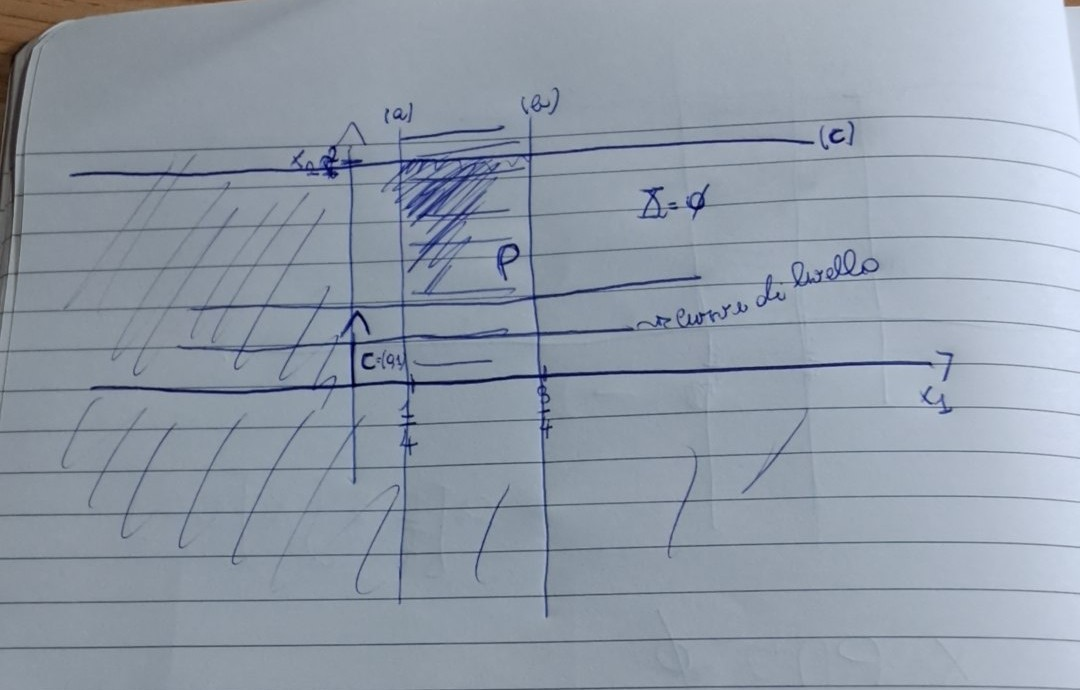
\includegraphics[width=0.8\textwidth]{_files/_images/photo_2026-11-12_17-15-25.jpg}
    \caption{Regione ammissibile del rilassamento nell'esempio:
\(x^*\notin\mathbb Z^2\) e il vettore arrotondato \(x^I\notin X\).
Il problema intero ha \(X=\varnothing\); la freccia della funzione
obiettivo indica il verso di crescita di \(x_2\).}
    \label{fig:immagine}
\end{figure}


\subsection{Relazioni fra un problema di PLI ed il suo rilassamento continuo}

Siano (Pli) un problema di programmazione lineare intera con regione ammissibile $X$, $X^*$ insieme di soluzioni ottime e sia $z^*_{(Pli)}$ il valore ottimo della funzione obiettivo,sempre nel problema di programmazione lineare intera.
Consideriamo poi (Pli-c) il suo rilassamento continuo con regione ammissibile $P$,$P^*$ l'insieme di soluzioni ottime e il valore ottimo della funzione obiettivo del Pli-c, come $z^*_{(Pli-c)}$

\begin{proposition}{Relazioni fondamentali}
Fra il problema intero e il suo rilassamento valgono le seguenti relazioni.
\begin{enumerate}
\item \(P=\varnothing\Longrightarrow X=\varnothing\):
se il rilassamento è inammissibile, lo è anche il problema intero.

\item Se il problema intero è illimitato nel verso di ottimizzazione,
anche il rilassamento è illimitato nello stesso verso.
Per un problema di minimo,
\[
z^*_{(Pli)} = -\infty \implies z^*_{(Pli-c)} = -\infty  
\]
Per un problema di massimo, l'analoga relazione usa \(+\infty\).

\item Se \(P^*\neq\varnothing\) (cioè appartiene all'insieme delle soluzioni ottime) e \(X^*\neq\varnothing\), nel caso
di minimo si ha il lower bound
\[
z^*_{(\mathrm{Pli\text{-}c})}\leq z^*_{(\mathrm{Pli})}.
\]
Questo perchè $P$ è piu grande ed è un sottoinsieme di $X$


\item Se \(y\in P^*\) e \(y\in\mathbb Z^n\), allora
\[
y\in X^*,\qquad
z(y)=z^*_{(\mathrm{Pli\text{-}c})}=z^*_{(\mathrm{Pli})}.
\]

\item Può accadere che
\[
X=\varnothing,\qquad P^*\neq\varnothing.
\]
È il caso dell'esempio precedente: il problema intero è inammissibile,
ma il rilassamento possiede un ottimo finito.

\item Può accadere che \(X=\varnothing\) e il rilassamento sia illimitato.
Un esempio è
\begin{align*}
\max\quad &x_2\\
\text{s.a.}\quad
&x_1\geq\frac14 &&\text{(a)},\\
&x_1\leq\frac34 &&\text{(b)},\\
&x_1,x_2\geq0,\qquad x_1,x_2\in\mathbb Z.
\end{align*}
Qui \(X=\varnothing\), mentre nel rilassamento continuo il valore della funzione obiettivo può crescere illimitatamente verso + $\infty$.
Questo perchè la regione ammissibile $P$ è illimtata verso l'alto, come vedi sotto.
\end{enumerate}
\end{proposition}



\begin{center}
\begin{minipage}{\linewidth}
\centering
\captionsetup{hypcap=false}
\begin{tikzpicture}[x=3.8cm,y=1.2cm,>=Stealth,font=\small]
  \fill[blue!7] (.25,0) rectangle (.75,3.2);
  \draw[->] (-.13,0)--(1.65,0) node[right] {$x_1$};
  \draw[->] (0,-.25)--(0,3.3) node[above] {$x_2$};
  \draw[->] (.25,-.12)--(.25,3.15) node[above] {(a)};
  \draw[->] (.75,-.12)--(.75,3.15) node[above] {(b)};
  \draw[->] (.25,2.8)--(.43,2.8);
  \draw[->] (.75,2.6)--(.57,2.6);
  \draw[brown!70!black] (-.1,1.6)--(1.5,1.6);
  \draw[->,brown!70!black] (1.4,1.6)--(1.4,2)
    node[right] {f.o.};
  \foreach \x/\lab in {.25/{\frac14},.5/{\frac12},.75/{\frac34},1/1} {
    \draw (\x,.035)--(\x,-.035);
    \node[below] at (\x,-.04) {$\lab$};
  }
  \foreach \y in {1,2} \node[left] at (0,\y) {$\y$};
  \node at (.5,1.1) {$P$};
  \node at (1.12,.65) {$X=\varnothing$};
\end{tikzpicture}
\captionof{figure}{Regione del rilassamento nel caso 6: la striscia
\(\frac14\leq x_1\leq\frac34,\ x_2\geq0\) è illimitata verso l'alto
ma non contiene punti interi. Quindi \(X=\varnothing\), mentre
il rilassamento di massimo ha valore \(+\infty\).}
\label{fig:striscia-illimitata}
\end{minipage}
\end{center}

\subsection{Matrice dei vincoli unimodulare}
\label{subsec:unimodularita}

In generale l'ottimo del rilassamento non risolve direttamente
il problema intero. Esistono però strutture della matrice dei vincoli
che garantiscono l'interezza delle soluzioni di base, quando
i termini noti sono interi.

\begin{definition}{Matrice unimodulare}
Una matrice intera \(A\in\mathbb Z^{m\times n}\), con \(m\leq n\),
si dice \emph{unimodulare}, nella terminologia adottata nel testo,
se ogni sua sottomatrice quadrata \(B\in\mathbb Z^{m\times m}\)
soddisfa
\[
\det(B)\in\{-1,0,1\}.
\]
\end{definition}


Supponiamo di dover risolvere un problema di programmazione lineare intera (Pli), in cui la matrice dei vincoli \(A\) e il vettore dei termini noti \(b\) abbiano elementi interi.

Consideriamo ora il rilassamento continuo associato al problema (Pli) e supponiamo che \(x^*\) sia una sua soluzione ottima del problema.

Vogliamo stabilire sotto quali condizioni \(x^*\) abbia tutte le componenti intere, così da poter concludere che \(x^*\) è anche una soluzione ottima del problema originale (Pli).

\begin{warning}{}
  Prima di procedere, ricordati un teorema fondamentale,se un problema di programmazione lineare in forma standard (in questo caso il rilassamento continuo),
  ammette una soluzione ottima, allora esiste almeno una soluzione ottima che è una soluzione di base ammissibile (SBA).
\end{warning}

Noi quindi stiamo considerando $x^*$ come una soluzione ottima del problema, questa può essere o una soluzione ottima, o una SBA se è un vertice del poliedro, ma non una SB, perchè se fosse una SB e anche ottima, questo richiederebbe l'ammissibilità cioè sarebbe una SBA ottima.


Consideriamo quindi $x^*$,una SBA (dato che sappiamo che esiste dal teorema) (una SBA cioè stiamo considerando un vertice del poliedro), dato che una SBA è una soluzione di base, allora possiamo applicare il teorema \ref{teorema SBA}

\begin{warning}{}
  Nota che questo procedimento (cioè per dimostrare l'integrità) si può applicare a qualsiasi SBA, non perforza a SBA ottime del problema.
\end{warning}

Se \(B\) è la matrice di base associata alla soluzione $x^*$,
\[
x^*=
\begin{bmatrix}x_B^*\\x_N^*\end{bmatrix}
=
\begin{bmatrix}B^{-1}b\\0\end{bmatrix}.
\]
Le componenti non di base sono già intere perché nulle.
L'interezza di \(x^*\) dipende dunque da \(B^{-1}b\).
Poiché \(b\in\mathbb Z^m\) (abbiamo presupposto che $A$ e $b$ fossero interi), una condizione sufficiente è che
\(B^{-1}\) sia intera.

Per definizione si ha che:
\[
B^{-1}
=\frac{1}{\det(B)}
\begin{bmatrix}
\alpha_{11}&\alpha_{12}&\cdots&\alpha_{1m}\\
\alpha_{21}&\alpha_{22}&\cdots&\alpha_{2m}\\
\vdots&\vdots&\ddots&\vdots\\
\alpha_{m1}&\alpha_{m2}&\cdots&\alpha_{mm}
\end{bmatrix}^{\mathsf T},
\]
dove
\[
\alpha_{ij}=(-1)^{i+j}\det(M_{ij})
\]
e \(M_{ij}\) si ottiene da \(B\) eliminando la riga \(i\)
e la colonna \(j\).

La matrice \(B\) è intera perché è estratta da \(A\).
Ogni \(M_{ij}\) è intera, quindi il suo determinante (det($M_{i,j}$)) e
il cofattore \(\alpha_{ij}\) sono interi.

Quindi $B^{-1}$ è intera se il determinante di $B$ è -1 o 1:
\[
\det(B)\in\{-1,1\},
\]

Quindi :
\[
\det(B)\in\{-1,1\} \implies x^* \in \mathbb{Z}^n
\]
E quindi $x^*$ è una soluzione ottima anche del problema originale.
\textbf{$x^*$ era una SBA e quindi un vertice del poliedro del problema di rilassamento, e abbiamo dimostrato che era intero}

Da questo possiamo generalizzare a tutti i vertici del poliedro e dire questo teorema:
\begin{theorem}{Interezza dei vertici}
\label{thm:vertici-interi}
Sia \(A\in\mathbb Z^{m\times n}\) unimodulare e di rango \(m\),
e sia \(b\in\mathbb Z^m\). Allora il poliedro
\[
P=\{x\in\mathbb R^n:Ax=b,\ x\geq0\}
\]
ha soltanto vertici interi.
\end{theorem}

\begin{proof}
Ogni vertice del poliedro in forma standard è una soluzione
di base ammissibile. La sua matrice di base \(B\) è non singolare (cioè il determinante è diverso da 0, questo per la definizione di prima della matrice inversa, dato che il determinante sta del denominatore)
e, dato che per l'unimodularità di \(A\) allora il determinante può assumere questi valori,
\[
\det(B)\in\{-1,0,1\}\setminus\{0\}=\{-1,1\}.
\]
Grazie a prima possiamo dire che  \(B^{-1}\) è intera.
Segue \(x_B=B^{-1}b\in\mathbb Z^m\); inoltre \(x_N=0\).
Ogni vertice appartiene quindi a \(\mathbb Z^n\).
\end{proof}


Se il rilassamento ha un ottimo finito, se ne può scegliere uno
di base: sotto le ipotesi del teorema è intero e risolve
anche il problema di PLI.


\newpage

\subsubsection*{Esempi di problemi di PLI con matrice dei vincoli unimodulare}

Due problemi classici hanno una struttura particolarmente favorevole:
il \emph{Problema del Trasporto} e il \emph{Problema dell'Assegnamento}.
In entrambi i termini noti sono interi e la matrice dei vincoli
possiede una proprietà ancora più forte dell'unimodularità,
che sarà dimostrata di seguito.

\subsubsection{Il Problema del Trasporto: problema di Hitchcock}
\label{ex:trasporto}
Sono dati \(m\) fornitori di un bene \(M\) e \(n\) clienti.
Il fornitore \(i\), con \(i=1,\ldots,m\), dispone di
\(s_i\in\mathbb Z_{\geq0}\) unità di bene; il cliente \(j\),
con \(j=1,\ldots,n\), richiede \(d_j\in\mathbb Z_{\geq0}\) unità.
Il costo di trasporto di un'unità dal fornitore \(i\) al cliente \(j\)
è \(c_{ij}\). Si assume inizialmente il \emph{bilanciamento}:
\begin{equation}
\sum_{i=1}^m s_i=\sum_{j=1}^n d_j.
\tag{3.1}\label{eq:bilanciamento}
\end{equation}
\textbf{cioè c'è merce per tutti, ma senza ecceddere}.\\

L'obiettivo è minimizzare il \textbf{costo totale del trasporto rispettando}
le disponibilità dei fornitori e le richieste dei clienti.

Indichiamo con \(f_{ij}\) la quantità \textbf{trasportata} dal fornitore \(i\) al cliente \(j\).
La formulazione è
\begin{align*}
\min\quad &\sum_{i=1}^m\sum_{j=1}^n c_{ij}f_{ij} = c_{11} f_{11} + c_{12} f_{12} \dots \text{ $c$ è un pò come un termine di peso, fissato all'inizio}\\
\text{s.a.}\quad
&\sum_{i=1}^m f_{ij}=d_j \text{ cioè i clienti vengono soddisfati tutti},
&&j=1,\ldots,n \quad \text{(a)},\\
&\sum_{j=1}^n f_{ij}=s_i \text{ cioè i fornitori devono usare tutto il loro bene disponibile e darlo ai clienti},
&&i=1,\ldots,m \quad \text{(b)},\\
&f_{ij}\geq0,
i=1,\ldots,m,j=1,\ldots,n.
\end{align*}


\begin{warning}{}
    Ovviamente, possono esistere diverse soluzioni ammissibili al problema, che differiscono per le quantità di merce trasportate lungo i vari percorsi. Dobbiamo quindi determinare quanta merce trasportare da ciascun fornitore a ciascun cliente, rispettando i vincoli di disponibilità e di domanda, in modo da minimizzare il costo totale del trasporto.
\end{warning}
\begin{observation}{}
    Ogni valore assunto dall'indice $j=1,\dots,n$ identifica un vincolo distinto e, di conseguenza, una riga della matrice $A$.

    In particolare, a $j=1$ corrisponde il primo vincolo, a $j=2$ il secondo, e così via, fino a ottenere $n$ vincoli.

    Analogamente, ogni valore dell'indice $i=1,\dots,m$ identifica un ulteriore vincolo, per un totale di $m$ vincoli.

    Complessivamente, si ottengono quindi $m+n$ vincoli, corrispondenti alle $m+n$ righe della matrice $A$.
\end{observation}

I vincoli (a) sono i \emph{vincoli di destinazione}, cioè che il cliente riceve tutto quello che richiede da i diversi fornitori (può essere anche uno solo) ad es.
\[
d_1 = f_{11} + f_{21} + \dots
\]
Cioè la richiesta di quel cliente, può essere fornita da diversi fornitori


i vincoli (b) sono i \emph{vincoli di origine} cioè che i fornitori forniscano tutto quello che hanno ai clienti (posso fornire anche tutto ad un solo cliente) ad es. 
\[
s_1 = f_{11} + f_{12} + \dots
\]
cioè il fornitore da tutto quello che ha ai vari clienti.




Quello che vogliamo determinare attraverso la risoluzione del problema è il vettore delle variabili decisionali $f$, che in questo caso svolge il ruolo del vettore $x$ di un generico problema di programmazione lineare.

In particolare, vogliamo trovare un vettore $f$ che specifichi quanta merce trasportare lungo ciascun percorso fornitore-cliente, in modo da minimizzare il costo totale del trasporto, rispettando tutti i vincoli del problema.

Il vettore $f$ ha dimensione $mn$, poiché contiene una variabile $f_{ij}$ per ogni possibile coppia fornitore-cliente, con $i=1,\dots,m$ e $j=1,\dots,n$.



\newpage

Si osservi quanto segue.
\begin{enumerate}
\item[i.] Le variabili di decisione $f_{ij}$ sono $m \times n$.
\begin{observation}{}
  Questo perchè per ogni fornitore, dobbiamo modellare con le variabili di decisione $n$ clienti, ad esempio per il fornitore 1, abbiamo:
  \[
  f_{11},f_{12},\dots,f_{1n}
  \]
  ci sono $m$ fornitori e quindi abbiamo $m \times n$ variabili.
\end{observation}

\item[ii.] Sommando i vincoli di destinazione e quelli di origine,
\[
\sum_{j = 1}^{n} \sum_{i = 1}^{m} f_{ij} = \sum_{i = 1}^{m} \sum_{j = 1}^{n} f_{ij} \implies \sum_{j = 1}^{n} d_j = \sum_{i = 1}^{m} s_i  
\]
Il bilanciamento \eqref{eq:bilanciamento} è quindi necessario
per l'ammissibilità del modello con tutte le uguaglianze.

\item[iii.] La matrice dei vincoli è unimodulare e
con \(s_i,d_j\) interi, ogni soluzione di base ammissibile
è intera (\textbf{dal teorema di interezza dei vertici}).


\begin{definition}{Grafo Bipartito}
Un grafo bipartito è un grafo \(G=(V,E)\) in cui l'insieme dei vertici \(V\) può essere suddiviso in due sottoinsiemi disgiunti \(V_1\) e \(V_2\), tali che:
\begin{enumerate}
  \item \(V_1 \cup V_2 = V\)
  \item \(V_1 \cap V_2 = \varnothing\)
  \item Ogni arco collega un vertice di \(V_1\) con un vertice di \(V_2\).
\end{enumerate}
Un grafo è Bipartito completo, se ogni vertice di \(V_1\) è collegato a ogni vertice di \(V_2\)
\end{definition}

\item[iv.] Ogni istanza si rappresenta con un grafo bipartito completo, l'istanza del grafo è:
\[
K_{m,n}=(F\cup C,E),
\]
nel quale:
\begin{itemize}
\item \(F=\{1,\ldots,m\}\) è l'insieme dei fornitori;
\item \(C=\{1,\ldots,n\}\) è l'insieme dei clienti, distinto da \(F\);
\item \(E=\{[i,j]:i\in F,\ j\in C\}\);
\item \(c:E\longrightarrow\mathbb R_{\geq0}\) associa
il costo \(c_{ij}\) al collegamento \([i,j]\).
\end{itemize}
Le frecce nelle figure indicano il trasporto dal fornitore
al cliente.
\end{enumerate}

\begin{center}
\begin{minipage}{\linewidth}
\centering
\captionsetup{hypcap=false}
\begin{tikzpicture}[>=Stealth,font=\small,
  forn/.style={circle,draw=blue!65!black,minimum size=7mm,inner sep=1pt},
  cli/.style={circle,draw=red!70!black,minimum size=7mm,inner sep=1pt}]
  \node[forn] (f1) at (0,3.6) {$1$};
  \node[forn] (fi) at (0,1.8) {$i$};
  \node[forn] (fm) at (0,0) {$m$};
  \node[cli] (c1) at (5,3.6) {$1$};
  \node[cli] (cj) at (5,1.8) {$j$};
  \node[cli] (cn) at (5,0) {$n$};
  \node[above,blue!65!black] at (f1.north) {$F$};
  \node[above,red!70!black] at (c1.north) {$C$};
  \foreach \f in {f1,fi,fm}
    \foreach \c in {c1,cj,cn}
      \draw[->,gray!75] (\f)--(\c);
  \draw[->] (fi)--node[above,fill=white,inner sep=2pt] {$c_{ij}$}(cj);
  \node at (0,2.7) {$\vdots$};
  \node at (0,.9) {$\vdots$};
  \node at (5,2.7) {$\vdots$};
  \node at (5,.9) {$\vdots$};
\end{tikzpicture}
\captionof{figure}{Grafo bipartito completo rappresentante una generica istanza
del Problema del Trasporto. Ogni fornitore è collegato a ogni cliente;
il collegamento \([i,j]\) ha costo \(c_{ij}\).}
\label{fig:trasporto-generico}
\end{minipage}
\end{center}

La matrice dei coefficienti tecnologici ha dimensioni
\[
(m+n)\times mn
\]
\begin{warning}{}
    Questo perché:
    \begin{enumerate}
        \item \textbf{Numero di righe: $m+n$.}
        Ogni riga della matrice corrisponde a un vincolo del problema.
        In particolare:
        \begin{itemize}
            \item Abbiamo $n$ vincoli relativi alla domanda dei clienti, uno per ciascun cliente $j=1,\dots,n$.
            \item Abbiamo $m$ vincoli relativi alla disponibilità dei fornitori, uno per ciascun fornitore $i=1,\dots,m$.
        \end{itemize}
        Pertanto, il numero complessivo di righe è $m+n$.

        \item \textbf{Numero di colonne: $mn$.}
        Ogni colonna corrisponde a una variabile decisionale $f_{ij}$, che rappresenta la quantità di merce trasportata dal fornitore $i$ al cliente $j$.

        Poiché abbiamo $m$ fornitori e $n$ clienti, esistono $mn$ possibili coppie fornitore-cliente e, quindi, $mn$ variabili decisionali.

        Questo rappresenta tutte le possibili coppie fornitore-clienti che possono essere messe sulle colonne
    \end{enumerate}
\end{warning}
e coincide con la matrice di incidenza nodo--arco \emph{non orientata}
del grafo bipartito

Consideriamo concretamente \(m=3\) fornitori e \(n=2\) clienti:
\begin{align*}
\min\quad
&c_{11}f_{11}+c_{12}f_{12}
+c_{21}f_{21}+c_{22}f_{22}
+c_{31}f_{31}+c_{32}f_{32}\\
\text{s.a.}\quad
&f_{11}+f_{12}=s_1,\\
&f_{21}+f_{22}=s_2,\\
&f_{31}+f_{32}=s_3,\\
&f_{11}+f_{21}+f_{31}=d_1,\\
&f_{12}+f_{22}+f_{32}=d_2,\\
&f_{ij}\geq0,\qquad i=1,2,3,\quad j=1,2.
\end{align*}
Nell'ordine di colonne
\[
f_{11},\ f_{12},\ f_{21},\ f_{22},\ f_{31},\ f_{32},
\]
la matrice è
\[
A=
\begin{bmatrix}
1&1&0&0&0&0\\
0&0&1&1&0&0\\
0&0&0&0&1&1\\
1&0&1&0&1&0\\
0&1&0&1&0&1
\end{bmatrix}\in\mathbb Z^{5\times6}.
\]
il vettore decisionale è
\[
f = \begin{pmatrix}
f_{11} \\
 f_{12} \\
 \vdots \\
 f_{mn}
\end{pmatrix}
\]

Le prime tre righe rappresentano i fornitori, le ultime due
i clienti. Il grafo associato è \(K_{3,2}\), con
\(F=\{1,2,3\}\) e \(C=\{1,2\}\).

\begin{center}
\begin{minipage}{\linewidth}
\centering
\captionsetup{hypcap=false}
\begin{tikzpicture}[>=Stealth,font=\small,
  forn/.style={circle,draw=blue!65!black,minimum size=8mm},
  cli/.style={circle,draw=red!70!black,minimum size=8mm}]
  \node[forn] (f1) at (0,4) {$1$};
  \node[forn] (f2) at (0,2) {$2$};
  \node[forn] (f3) at (0,0) {$3$};
  \node[cli] (c1) at (5,3.5) {$1$};
  \node[cli] (c2) at (5,.5) {$2$};
  \node[above,blue!65!black] at (f1.north) {$F$};
  \node[above,red!70!black] at (c1.north) {$C$};
  \draw[->] (f1)--node[pos=.35,above,fill=white,inner sep=1pt] {$c_{11}$}(c1);
  \draw[->] (f1)--node[pos=.25,below,fill=white,inner sep=1pt] {$c_{12}$}(c2);
  \draw[->] (f2)--node[pos=.3,above,fill=white,inner sep=1pt] {$c_{21}$}(c1);
  \draw[->] (f2)--node[pos=.32,below,fill=white,inner sep=1pt] {$c_{22}$}(c2);
  \draw[->] (f3)--node[pos=.24,above,fill=white,inner sep=1pt] {$c_{31}$}(c1);
  \draw[->] (f3)--node[pos=.35,below,fill=white,inner sep=1pt] {$c_{32}$}(c2);
\end{tikzpicture}
\captionof{figure}{Grafo \(K_{3,2}\) dell'istanza del trasporto con tre fornitori
e due clienti. Sono rappresentati tutti i sei collegamenti
e i rispettivi costi.}
\label{fig:trasporto-32}
\end{minipage}
\end{center}

\newpage

\paragraph{Importanti osservazioni.}

La prima importante osservazione riguarda l'ipotesi di bilanciamento, che risulta essere non restrittiva.

Questo significa che, anche qualora il problema originale non fosse bilanciato, sarebbe comunque possibile ricondurlo a un problema bilanciato equivalente, senza compromettere la ricerca di una soluzione ottima.

Si considerino, infatti, i seguenti due scenari alternativi:


\paragraph{Scenario 1: offerta complessiva inferiore alla domanda}
Supponiamo che
\[
\sum_{i=1}^m s_i<\sum_{j=1}^n d_j.
\]
I fornitori reali non possono soddisfare tutta la domanda.
Per i soli flussi reali si considera quindi
\[
\sum_{i=1}^m f_{ij}\leq d_j,\qquad j=1,\ldots,n.
\]
Cioè per alcuni clienti potrebbe essere minore, per alcuni uguale e soddisfarli.


Questo non va bene perchè non rispetta il vincolo (a) che avevamo messo nel problema standard, quindi faremo in modo di bilanciarlo. 
\\
\textbf{Questo viola il vincolo (a), quindi come si fa a bilanciarlo?}
\\
Si procede così:
\begin{enumerate}
\item si introduce un fornitore fittizio \(m+1\) nell'insieme dei fornitori;
\item si introducono \(n\) ulteriori variabili
\[
f_{(m+1)j}\geq0,\qquad j=1,\ldots,n;
\]
\item si definiscono la disponibilità del nuovo fornitore fittizio e i suoi costi:
\[
\begin{aligned}
s_{m+1} &= \sum_{j=1}^n d_j-\sum_{i=1}^m s_i,
\\
\\[6pt]
c_{(m+1)j} &= \text{da definire},\qquad j=1,\ldots,n.
\end{aligned}
\]
cioè la disponibilità del fornitore fittizio viene definita come la quantità di merce necessaria a soddisfare la domanda complessiva che non può essere coperta dagli altri fornitori.
\end{enumerate}
Il modello bilanciato risultante è
\begin{align*}
\min\quad &\sum_{i=1}^{m+1}\sum_{j=1}^n c_{ij}f_{ij}\\
\text{s.a.}\quad
&\sum_{j=1}^n f_{ij}=s_i,
&&i=1,\ldots,m+1 \qquad\text{(a)},\\
&\sum_{i=1}^{m+1}f_{ij}=d_j,
&&j=1,\ldots,n \qquad\text{(b)},\\
&f_{ij}\geq0,
&&i=1,\ldots,m+1,\quad j=1,\ldots,n.
\end{align*}
La quantità \(f_{(m+1)j}\) che compare sopratutto nel vincolo (a) misura la domanda del cliente \(j\)
non soddisfatta dai fornitori reali. Questo perchè devi pensarlo cosi, quando arriva $i=m+1$, si ha
\[
s_{m+1} = f_{m+1,1} + f_{m+1,2} + \dots + f_{m+1,n}
\]
ed ognuno misura la quantità non soddisfata dai fornitori reali, che verrà soddisfatta da questo.


\newpage

\paragraph{Scenario 2: offerta complessiva superiore alla domanda}
Supponiamo che
\[
\sum_{i=1}^m s_i>\sum_{j=1}^n d_j.
\]
Cioè la disponibilità di fornitura, è maggiore della domanda degli utenti.


Succede quindi che \textbf{qualche} fornitore può spedire meno della propria disponibilità:
\[
\sum_{j=1}^n f_{ij}\leq s_i,\qquad i=1,\ldots,m.
\]
Cioè un fornitore spartenedo la sua merce a tutti i clienti potrebbe non esaurire la quantità che ha disposizione.
\textbf{Questo viola il vincolo (b), quindi come si fa a bilanciarlo?}
\\
Si procede così:
\begin{enumerate}
\item si introduce un cliente fittizio \(n+1\);
\item si introducono \(m\) ulteriori variabili
\[
f_{i(n+1)}\geq0,\qquad i=1,\ldots,m;
\]
\item si definiscono la sua domanda e i suoi costi:
\[
d_{n+1}=\sum_{i=1}^m s_i-\sum_{j=1}^n d_j,
\qquad
c_{i(n+1)}\ \text{da definire},\quad i=1,\ldots,m.
\]
\textbf{Questo cliente quindi prenderà tutto quello che hanno in piu gli altri fornitori}
\end{enumerate}
Il modello bilanciato è
\begin{align*}
\min\quad &\sum_{i=1}^m\sum_{j=1}^{n+1}c_{ij}f_{ij}\\
\text{s.a.}\quad
&\sum_{j=1}^{n+1}f_{ij}=s_i,
&&i=1,\ldots,m \qquad\text{(a)},\\
&\sum_{i=1}^m f_{ij}=d_j,
&&j=1,\ldots,n+1 \qquad\text{(b)},\\
&f_{ij}\geq0,
&&i=1,\ldots,m,\quad j=1,\ldots,n+1.
\end{align*}
Il flusso verso il cliente fittizio rappresenta l'offerta inutilizzata.
Il relativo costo può essere nullo oppure descrivere, per esempio,
costi di stoccaggio o smaltimento.


\textbf{Quindi in tutti e due i casi abbiamo bilanciato il problema, facendo in modo che rispettasero i vincoli (a) e (b)}


La seconda osservazione riguarda l'esistenza di un ottimo finito.

\newpage

\begin{theorem}{Esistenza di un ottimo finito per il trasporto}
\label{thm:trasporto-ottimo}
Ogni istanza \textbf{bilanciata} del Problema del Trasporto
ammette almeno una soluzione ottima finita.
\end{theorem}

\begin{proof}
Poniamo
\[
\alpha=\sum_{i=1}^m s_i=\sum_{j=1}^n d_j.
\]
Definiamo
\begin{equation}
f_{ij}=\frac{s_i d_j}{\alpha},
\qquad i=1,\ldots,m,\quad j=1,\ldots,n.
\tag{3.2}\label{eq:soluzione-proporzionale}
\end{equation}
Tali quantità sono nonnegative. Ora abbiamo dato un assegnamento alla quantità trasportata, vediamo se queste quantità soddisfano i vincoli.
Per ogni fornitore \(i\), i vincoli di origine sono soddisfatti:
\begin{align*}
\sum_{j=1}^n f_{ij}
&=\sum_{j=1}^n\left(\frac{s_i d_j}{\sum_{r=1}^m s_r}\right)\\
&=\frac{s_i}{\sum_{r=1}^m s_r}\sum_{j=1}^n d_j\\
&=\frac{s_i}{\alpha}\,\alpha
\qquad\text{per il bilanciamento}\\
&=s_i.
\end{align*}
Per ogni cliente \(j\), i vincoli di destinazione sono soddisfatti:
\begin{align*}
\sum_{i=1}^m f_{ij}
&=\sum_{i=1}^m\left(\frac{s_i d_j}{\sum_{\ell=1}^n d_\ell}\right)\\
&=\frac{d_j}{\sum_{\ell=1}^n d_\ell}\sum_{i=1}^m s_i\\
&=\frac{d_j}{\alpha}\,\alpha
\qquad\text{per il bilanciamento}\\
&=d_j.
\end{align*}
La soluzione \eqref{eq:soluzione-proporzionale} è ammissibile.
Quindi abbiamo dimostrato che la regione ammissibile è non vuota e può contenere questa soluzione, quindi sicuramente è non vuota.


Poi per ogni soluzione ammissibile (immagina ce ne siano tante) e per ogni \(i,j\), si ha inoltre
\begin{align*}
&f_{ij}\geq0,\\
&\sum_{j=1}^n f_{ij}=s_i
\quad\Longrightarrow\quad f_{ij}\leq s_i, \forall i,j\\
&\sum_{i=1}^m f_{ij}=d_j
\quad\Longrightarrow\quad f_{ij}\leq d_j \forall i,j.
\end{align*}
Quindi
\[
0\leq f_{ij}\leq\min\{s_i,d_j\}.
\]
La funzione obiettivo, essendo lineare, è continua. Poiché la regione ammissibile è non vuota e compatta, per il teorema di Weierstrass la funzione obiettivo assume su di essa un minimo e un massimo assoluti. Di conseguenza, possiamo affermare che esiste almeno una soluzione ottima finita, anche se non sappiamo ancora quale sia
\end{proof}


\newpage
La terza osservazione riguarda la matrice dei coefficienti tecnologici.
Per il trasporto si può dimostrare la \emph{totale unimodularità},
che riguarda tutti i minori quadrati, non soltanto quelli
di ordine massimo.

\begin{definition}{Matrice totalmente unimodulare}
Una matrice intera \(A\in\mathbb Z^{m\times n}\), con \(m\leq n\),
si dice \emph{totalmente unimodulare} se, per \textbf{ogni sottomatrice
quadrata} \(B\) di qualunque ordine \(k=1,\ldots,m\), vale
\[
\det(B)\in\{-1,0,1\}.
\]

\end{definition}

\begin{remark}{Chiarimento sulla differenza fra le due proprietà}
La totale unimodularità implica l'unimodularità nella definizione.
\end{remark}

\begin{theorem}{Totale unimodularità della matrice del trasporto}
\label{thm:trasporto-tu}
Sia \(A\) la matrice dei coefficienti tecnologici del Problema
del Trasporto. Per ogni sua sottomatrice quadrata \(A^{(k)}\)
di ordine \(k\), vale
\[
\det\!\left(A^{(k)}\right)\in\{-1,0,1\}.
\]
Quindi \(A\) è totalmente unimodulare.
\end{theorem}

\begin{proof}
Ogni colonna di \(A\), corrispondente a \(f_{ij}\), contiene
esattamente due \(1\): uno in una riga di origine e uno
in una riga di destinazione. Gli altri elementi sono nulli.
Una colonna di \(A^{(k)}\) può dunque contenere zero, uno o due \(1\).

Procediamo per induzione sull'ordine \(k\). Per \(k=1\), l'elemento
è \(0\) o \(1\), quindi l'affermazione è vera.
Per \(k>1\), distinguiamo i tre casi del testo.
\begin{enumerate}
\item \textbf{Esiste una colonna interamente nulla.}, basta che una fra le colonne è interamente nulla
Il determinante è immediatamente nullo:
\[
\det\!\left(A^{(k)}\right)=0.
\]

\item \textbf{Ogni colonna contiene due \(1\).}
Sono presenti entrambi gli estremi di ciascun arco selezionato.
La somma delle righe di origine coincide con quella
delle righe di destinazione: ciascuna colonna contribuisce
con un \(1\) a entrambe. Le righe sono linearmente dipendenti
e il determinante è nullo.

L'esempio del testo, con tre fornitori e due clienti, è
\[
A=
\begin{bmatrix}
1&1&0&0&0&0\\
0&0&1&1&0&0\\
0&0&0&0&1&1\\
1&0&1&0&1&0\\
0&1&0&1&0&1
\end{bmatrix}
\quad\Longrightarrow\quad
A^{(4)}=
\begin{bmatrix}
1&1&0&0\\
0&0&1&1\\
1&0&1&0\\
0&1&0&1
\end{bmatrix}.
\]
Le prime due righe di \(A^{(4)}\) sono di origine e le ultime
due di destinazione. Le somme sono
\[
\begin{array}{rrrr@{\quad}c}
1&1&0&0&+\\
0&0&1&1&\\ \cline{1-4}
1&1&1&1&
\end{array}
\qquad\qquad
\begin{array}{rrrr@{\quad}c}
1&0&1&0&+\\
0&1&0&1&\\ \cline{1-4}
1&1&1&1&
\end{array}.
\]
Ne segue
\[
\text{riga}_1+\text{riga}_2-\text{riga}_3-\text{riga}_4=0,
\qquad \det\!\left(A^{(4)}\right)=0.
\]
Lo stesso ragionamento vale per qualunque \(k\) in questo caso.

\item \textbf{$A^{(k)}$ non ha alcuna colonna di tutti "0", ma almeno una colonna (eventualmente tutte) con un solo "1" (quindi eventualmente altre colonne possono avere tutti "1").}
Sviluppiamo il determinante lungo una di tali colonne.
Se l'\(1\) scelto (bisogna scegliere perforza un 1,per la regola del determinante) è nella posizione \((r,s)\), lo sviluppo
di Laplace dà
\[
\det\!\left(A^{(k)}\right)
=(-1)^{r+s}\det\!\left(A^{(k-1)}\right).
\]
Per solo ipotesi induttiva, \(\det\!\left(A^{(k-1)}\right)\in\{-1,0,1\}\); quindi anche
\(\det\!\left(A^{(k)}\right)\in\{-1,0,1\}\).

\end{enumerate}

\begin{example}{Esempio del terzo caso}
    
    \textbf{Esiste una colonna contenente esattamente
    un elemento uguale a $1$.}

    Escludendo i due casi precedenti, deve necessariamente
    esistere almeno una colonna contenente un solo $1$.

    In questo caso possiamo applicare lo
    \textbf{sviluppo di Laplace} lungo tale colonna,
    riducendo il calcolo del determinante a quello
    di una sottomatrice di ordine $k-1$.

    Consideriamo, ad esempio:

    \[
    A^{(3)}=
    \begin{pmatrix}
    0 & 1 & 1\\
    1 & 0 & 1\\
    0 & 1 & 0
    \end{pmatrix}.
    \]

    Osserviamo che la prima colonna contiene
    un solo elemento uguale a $1$, situato
    nella seconda riga.

    Sviluppando il determinante lungo questa colonna:

    \[
    \begin{aligned}
    \det(A^{(3)})
    &=(-1)^{2+1}
    \det
    \begin{pmatrix}
    1 & 1\\
    1 & 0
    \end{pmatrix}\\[6pt]
    &=-\left(1\cdot 0-1\cdot 1\right)\\[6pt]
    &=-(-1)\\[6pt]
    &=1.
    \end{aligned}
    \]

    Abbiamo quindi ottenuto:

    \[
    \boxed{\det(A^{(3)})=1.}
    \]

\textbf{Conclusione.}

I tre casi esaminati coprono tutte le possibilità,
poiché ogni colonna di $A^{(k)}$ può contenere
al massimo due elementi uguali a $1$.

Il caso base $k=1$ è immediato, poiché ogni
elemento della matrice originale appartiene
a $\{0,1\}$.

Per induzione, ogni sottomatrice quadrata
di $A$ ha determinante appartenente a
$\{-1,0,1\}$.

Possiamo quindi concludere che:

\[
\boxed{A \text{ è totalmente unimodulare}.}
\]

\end{example}

Quindi abbiamo dimostrato che ogni matrice quadrata che prendiamo (con $k > 1$), può ricadere nei 3 casi.

Nei primi due casi, è semplici da gestire, nell'ultimo caso si usa l'ipotesi di induzione.
\end{proof}

\begin{corollary}{Interezza delle soluzioni di base del trasporto}
\label{cor:trasporto-intero}
Se per ogni $i = 1,\dots,m$ e per ogni $j = 1,\dots,n$ si ha che $s_i$ e $d_j$ sono interi, allora ogni soluzione di base ammissibile del problema del trasporto è intera. 
\end{corollary}

\paragraph{Il Problema dell'Assegnamento}
\label{ex:assegnamento}
Il Problema dell'Assegnamento è il caso speciale del trasporto in cui:
\begin{enumerate}
\item[i.] \(m=n\): il numero di fornitori coincide con quello dei clienti;
\item[ii.] \(s_i=d_j=1\) per ogni \(i,j=1,\ldots,n\).
\end{enumerate}
La formulazione è
\begin{align*}
\min\quad &\sum_{i=1}^n\sum_{j=1}^n c_{ij}f_{ij}\\
\text{s.a.}\quad
&\sum_{i=1}^n f_{ij}=1,
&&j=1,\ldots,n \qquad\text{(a)},\\
&\sum_{j=1}^n f_{ij}=1,
&&i=1,\ldots,n \qquad\text{(b)},\\
&f_{ij}\geq0,
&&i=1,\ldots,n,\quad j=1,\ldots,n.
\end{align*}
La matrice è totalmente unimodulare e i termini noti
sono interi. Ogni soluzione di base ammissibile è dunque intera.
Dalle somme di riga (dei vincoli (a) e (b)) e dalla nonnegatività segue anche
\[
0\leq f_{ij}\leq1.
\]
Ogni soluzione di\textbf{ base ammissibile} (perchè intera) è perciò un vettore booleano,
con il significato
\[
f_{ij}=
\begin{cases}
1,&\text{se il fornitore \(i\) è assegnato al cliente \(j\)},\\
0,&\text{altrimenti}.
\end{cases}
\]
In particolare in una SBA \emph{intera}, fra le \(n^2\) ($mn$)
variabili esattamente \(n\) valgono \(1\) (\textbf{questo perchè fra gli $n$ clienti, posso ricevere in totale massimo $n$ oggetti}); le altre \(n^2-n\) valgono \(0\).
La matrice \((f_{ij})\) è una matrice di permutazione.

Ogni istanza si rappresenta con
\[
K_{n,n}=(F\cup C,E),
\]
nel quale:
\begin{itemize}
\item \(F=\{1,\ldots,n\}\) rappresenta i fornitori;
\item \(C=\{1,\ldots,n\}\) rappresenta i clienti ed è distinto da \(F\);
\item \(E=\{[i,j]:i\in F,\ j\in C\}\);
\item \(c:E\longrightarrow\mathbb R_{\geq0}\), con \(c([i,j])=c_{ij}\).
\end{itemize}
La matrice dei vincoli coincide con la matrice di incidenza
nodo--arco non orientata del grafo bipartito completo.
Una soluzione intera seleziona \(n\) collegamenti
che coprono ogni nodo una sola volta.

\begin{center}
\begin{minipage}{\linewidth}
\centering
\captionsetup{hypcap=false}
\begin{tikzpicture}[>=Stealth,font=\small,
  forn/.style={circle,draw=blue!65!black,minimum size=7mm},
  cli/.style={circle,draw=red!70!black,minimum size=7mm}]
  \node[forn] (f1) at (0,3.6) {$1$};
  \node[forn] (fi) at (0,1.8) {$i$};
  \node[forn] (fn) at (0,0) {$n$};
  \node[cli] (c1) at (5,3.6) {$1$};
  \node[cli] (cj) at (5,1.8) {$j$};
  \node[cli] (cn) at (5,0) {$n$};
  \node[above,blue!65!black] at (f1.north) {$F$};
  \node[above,red!70!black] at (c1.north) {$C$};
  \foreach \f in {f1,fi,fn}
    \foreach \c in {c1,cj,cn}
      \draw[->,gray!75] (\f)--(\c);
  \draw[->] (fi)--node[above,fill=white,inner sep=2pt] {$c_{ij}$}(cj);
  \node at (0,2.7) {$\vdots$};
  \node at (0,.9) {$\vdots$};
  \node at (5,2.7) {$\vdots$};
  \node at (5,.9) {$\vdots$};
\end{tikzpicture}
\captionof{figure}{Grafo bipartito completo di una generica istanza
del Problema dell'Assegnamento: entrambe le parti hanno \(n\) nodi
e il collegamento \([i,j]\) ha costo \(c_{ij}\).}
\label{fig:assegnamento}
\end{minipage}
\end{center}


\newpage

\section{Metodi dei Piani di Taglio}
\label{sec:piani-taglio}
Si consideri il problema di Programmazione Lineare Intera (Pli). Sia $P$ il poliedro regione ammissibile del suo rilassamento continuo (Pli-c)
e sia $X = P \cap \mathcal{Z}^n$ la regione ammissibile di (Pli). \\
Gli algoritmi appartenenti alla famiglia dei metodi dei piani di taglio iterativamente individuano la soluzione ottima $x^*$ del rilassamento continuo (Pli-c) e se $x^*$ \textbf{ha almeno una componente frazionaria} (quindi non è intero), essi \textbf{individuano un vincolo}
soddisfato da tutte le soluzioni intere del problema appartenenti alla regione ammissibile $P$ (cioè praticamente tutta la regione $X$), ma non soddisfato (\textbf{quindi violato}) dalla soluzione ottima $x^*$.
\textbf{Tale vincolo che abbiamo trovato}, viene aggiunto alla formulazione matematica di (Pli-c) è detto \textbf{taglio}.


In generale viene data la seguente definizione:
\begin{definition}{Taglio}
\label{def:taglio}
Dato \(x^*\in P\), il vincolo
\[
a^{\mathsf T}x\leq b_0
\]
è un taglio per \(x^*\) rispetto a \(X\) se:
\begin{enumerate}
\item[i.] Tutti i punti appartenenti all'insieme \(X\) rispettano il vincolo considerato.,
\[
a^{\mathsf T}x\leq b_0\qquad\forall x\in X;
\]
\item[ii.] è violata dal punto da eliminare,
\[
a^{\mathsf T}x^*>b_0.
\]
\end{enumerate}
\end{definition}

\begin{observation}{}
  Il vincolo, potrebbe essere anche un'uguaglianza o un >=, la prof. usa quello per rispettare una canonicità.
  Ricordarti ovviamente che anche se il (Pli-c) è fatto di altri tipo di vincoli (tipo >=), io posso sempre inserire il mio taglio, basta che rispetti la definizione.
\end{observation}


La prima condizione preserva tutte le soluzioni ammissibili
del problema intero, comprese quelle ottime.
La seconda elimina l'ottimo frazionario corrente.
Individuare un adeguato taglio è il \emph{problema della separazione}
di \(x^*\) da \(X\), che in generale può essere difficile
dal punto di vista computazionale.

\begin{center}
\begin{minipage}{\linewidth}
\centering
\captionsetup{hypcap=false}
\begin{tikzpicture}[x=1.04cm,y=.84cm,>=Stealth,font=\small]
  \fill[blue!5] (0,0)--(4.5,0)--(4.5,4)--(2.25,4.75)--(0,2.5)--cycle;
  \fill[red!14] (2,4.5)--(2.25,4.75)--(3,4.5)--cycle;
  \draw[->] (-.6,0)--(8,0) node[right] {$x_1$};
  \draw[->] (0,-.6)--(0,7.2) node[above] {$x_2$};
  \draw[gray] (-.55,1.95)--(5.1,7.6);
  \draw[gray] (-.55,5.6833)--(8,2.8333);
  \draw[gray] (4.5,-.45)--(4.5,7.2);
  \draw[->,gray] (4.8,7.3)--(5.4,6.7);
  \draw[->,gray] (7.2,3.1)--(7,2.45);
  \draw[->,gray] (-.3,2.2)--(.3,1.6);
  \foreach \i in {0,...,7} {
    \foreach \j in {0,...,6} {
      \fill[gray!55] (\i,\j) circle (1.25pt);
      \ifnum\i<5
        \pgfmathtruncatemacro{\amm}{(\j<=\i+2.5)&&(\j<=5.5-\i/3)}
        \ifnum\amm=1 \fill (\i,\j) circle (1.7pt); \fi
      \fi
    }
  }
  \draw[red!65!black] (-.5,4.5)--(8,4.5)
    node[right] {$a^{\mathsf T}x=b_0$};
  \fill (2.25,4.75) circle (2pt);
  \node[above left] at (2.25,4.75) {$x^*$};
  \foreach \i in {1,...,7} \node[below] at (\i,0) {\i};
  \foreach \j in {1,...,6} \node[left] at (0,\j) {\j};
  \node at (2.65,2.5) {$X$};
\end{tikzpicture}
\captionof{figure}{Il taglio \(a^{\mathsf T}x\leq b_0\) preserva tutti
i punti di \(X\) ed elimina \(x^*\). Nello schema il taglio
è orizzontale e la piccola porzione rossa viene esclusa.}
\label{fig:taglio-generico}
\end{minipage}
\end{center}

I metodi dei piani di taglio differiscono soprattutto per
il modo in cui risolvono il problema della separazione,
cioè per la scelta del vincolo aggiunto a ogni iterazione.
Lo schema generale è il seguente.

\begin{center}
\begin{minipage}{\linewidth}
\centering
\captionsetup{hypcap=false}
\fbox{\begin{minipage}{.94\linewidth}
\small
\textbf{algoritmo cutting-plane}\\[3pt]
\begin{tabular}{@{}r@{\quad}p{.86\linewidth}@{}}
1 & Dato \((\mathrm{Pli})\), trovare un ottimo \(x^*\)
del rilassamento \((\mathrm{Pli\text{-}c})\).\\[2pt]
2 & Porre \((\mathrm{Pli\text{-}c})_0:=(\mathrm{Pli\text{-}c})\),
\(x_0^*:=x^*\), \(k:=0\).\\[2pt]
3 & \textbf{while} \(x_k^*\) non è intero \textbf{do}\\
  & \quad individuare un taglio \(a_k^{\mathsf T}x\leq b_k\)
per \(x_k^*\);\\
  & \quad aggiungerlo a \((\mathrm{Pli\text{-}c})_k\),
ottenendo \((\mathrm{Pli\text{-}c})_{k+1}\);\\
  & \quad trovare un ottimo \(x_{k+1}^*\)
di \((\mathrm{Pli\text{-}c})_{k+1}\);\\
  & \quad porre \(k:=k+1\);\\
  & \textbf{endwhile}
\end{tabular}\\[3pt]
\textbf{end cutting-plane}
\end{minipage}}
\captionof{figure}{Schema del generico algoritmo dei piani di taglio,
con gli stessi passi dello pseudocodice del testo.}
\label{fig:algoritmo-cutting-plane}
\end{minipage}
\end{center}

Se si introduce un taglio per iterazione, il numero di iterazioni
del ciclo coincide con il numero di tagli aggiunti.
Intuitivamente, tagli più profondi possono ridurre il numero
di iterazioni; molti tagli ottenuti con le procedure classiche
eliminano però soltanto piccole porzioni del poliedro.
La profondità geometrica non garantisce, da sola,
un determinato numero di iterazioni.

\begin{remark}{Chiarimento sull'invariante e sulle condizioni dello schema}
Se \(P_k\) è la regione del rilassamento all'iterazione \(k\),
per ogni taglio valido si ha
\[
X\subseteq P_{k+1}\subseteq P_k,
\qquad
P_{k+1}\cap\mathbb Z^n=P_k\cap\mathbb Z^n=X.
\]

La seconda affermazione è vera perchè il vincolo nuovo aggiunto, mantiene dentro tutti i punti $X$. 

Per un problema di minimo con ottimi finiti,
\[
z^*_{(\mathrm{Pli\text{-}c})_0}
\leq z^*_{(\mathrm{Pli\text{-}c})_1}
\leq \cdots \leq z^*_{(\mathrm{Pli})}.
\]
Il miglioramento può non essere stretto, ad esempio in presenza
di ottimi multipli.

Lo pseudocodice presuppone che i rilassamenti considerati
abbiano un ottimo finito. Se, aggiungendo soltanto tagli validi,
un rilassamento diventa inammissibile, anche \(X\) è vuoto.
Se il rilassamento iniziale è illimitato, la sola procedura
scritta sopra non basta a classificare il problema intero.
Infine, lo schema astratto non costituisce di per sé
una dimostrazione di terminazione finita per qualunque
regola di generazione dei tagli.
\end{remark}

\newpage

\section{Branch e Bound}
\begingroup
\newcommand{\BBpli}[1]{\mathrm{PLI}_{#1}}
\newcommand{\BBrel}[1]{\mathrm{PLI}_{#1}\text{-c}}
\newcommand{\BBinc}{z_{\mathrm{opt}}}
\newcommand{\BBsol}{x_{\mathrm{opt}}}
\newcommand{\BBfig}[2]{%
  \par\nobreak\smallskip\nobreak
  {\small\textit{Figura #1 delle dispense.} #2\par}}

\subsection{Enumerazione implicita e partizione del problema}

\begin{definition}{Branch \& Bound}
Il Branch \& Bound (B\&B) è un metodo di enumerazione implicita per la
programmazione lineare intera (PLI), alternativo ai metodi dei piani di
taglio. Applica il principio \emph{divide and conquer}. La ramificazione
(\emph{branching}) suddivide il problema in sottoproblemi interi con
insiemi ammissibili più piccoli. La valutazione mediante limiti
(\emph{bounding}) permette di escludere interi sottoalberi quando nessuna
delle loro soluzioni può migliorare la migliore soluzione già trovata.
\end{definition}

\subsubsection{Una partizione in due sottoproblemi}

Sia $X$ l'insieme delle soluzioni intere ammissibili del problema richiamato
nella figura 3.10 delle dispense e sia $P$ la regione del suo rilassamento
continuo. Nella figura 3.11 il rilassamento ha soluzione ottima
\[
 x^*=\left(\frac32,2\right).
\]
La prima coordinata è frazionaria. Ogni soluzione intera deve avere
$x_1\leq 1$ oppure $x_1\geq 2$, poiché non esistono interi strettamente
compresi fra $1$ e $2$. Si costruiscono dunque due problemi distinti.
Nel primo si aggiunge alla formulazione originaria il solo vincolo
$x_1\leq 1$ e nel secondo il solo vincolo $x_1\geq 2$. Si ottengono
\[
 X_1=\{x\in X:x_1\leq 1\},\qquad X_2=\{x\in X:x_1\geq 2\},
\]
\[
 X_1\cup X_2=X,\qquad X_1\cap X_2=\varnothing.
\]
Entrambi i figli escludono $x^*$, mentre ogni soluzione intera del padre
appartiene a uno e un solo figlio. Indicando con $x^*_{x_1\leq 1}$
e $x^*_{x_1\geq 2}$ le rispettive soluzioni ottime, si sceglie quella
con il valore migliore della funzione obiettivo originaria.

\begin{center}
\begin{tikzpicture}[x=.90cm,y=.90cm,>=stealth,font=\small]
  \draw[->] (-.25,0)--(7,0) node[below left] {$x_1$};
  \draw[->] (0,-.22)--(0,4.2) node[left] {$x_2$};
  \draw[brown!65!black] (-.55,1.32)--(7,3.83);
  \draw[brown!65!black] (-.55,2.82)--(5.9,.24);
  \draw[brown!65!black] (1.15,-.425)--(7,2.5);
  \draw[->] (6.4,3.63)--(6.58,3.03);
  \draw[->] (6.1,2.05)--(5.90,2.45);
  \draw[->] (5,.60)--(4.82,.15);
  \draw[blue!60!black,very thick]
    (0,0)--(2,0)--(4,1)--(1.5,2)--(0,1.5)--cycle;
  \foreach \i in {0,...,4}{
    \foreach \j in {0,...,3}{
      \fill[brown!65!black] (\i,\j) rectangle ++(.085,.085);
    }
  }
  \foreach \i/\j in {0/0,0/1,1/0,1/1,2/0,2/1,3/1,4/1}
    \fill[red!70!black] (\i,\j) rectangle ++(.085,.085);
  \foreach \i in {1,2,3,4} \node[below] at (\i,-.04) {$\i$};
  \foreach \j in {1,2,3} \node[left] at (0,\j) {$\j$};
  \foreach \i in {1,2}
    \draw[green!55!black,very thick] (\i,-.10)--(\i,3.55);
  \draw[->,green!55!black] (1,3.35)--(.25,3.35);
  \draw[->,green!55!black] (2,3.35)--(2.76,3.35);
  \fill[blue!65!black] (1.5,2) circle (1.6pt) node[above=2pt] {$x^*$};
  \node[green!50!black] at (.51,.59) {$X_1$};
  \node[green!50!black] at (2.53,1.20) {$X_2$};
  \node[blue!65!black] at (3.65,1.70) {$P$};
\end{tikzpicture}
\BBfig{3.11}{Partizione mediante i vincoli $x_1\leq 1$ e $x_1\geq 2$.}
\end{center}

\subsubsection{Partizione generale e valore ottimo}

Si consideri il problema di minimo
\[
 (\BBpli{0})\qquad \min\{c^\top x:Ax\approx b,\ x\in\mathbb Z^n_{\geq 0}\}.
\]
Il simbolo $Ax\approx b$ raccoglie vincoli lineari il cui verso, per
ciascuna riga, può essere $\leq$, $=$ oppure $\geq$. Siano $X_0$ la
regione ammissibile, $z(x)=c^\top x$ e
$z^*_{\BBpli{0}}=\min_{x\in X_0}z(x)$.

\begin{definition}{Partizione della regione ammissibile}
I sottoproblemi $\BBpli{1},\ldots,\BBpli{n_0}$ costituiscono una
partizione del problema originario quando le loro regioni intere
$X_1,\ldots,X_{n_0}$ soddisfano
\[
 \bigcup_{i=1}^{n_0} X_i=X_0,\qquad X_i\cap X_j=\varnothing\quad(i\ne j).
\]
Si possono scartare i figli vuoti. La disgiunzione è richiesta per ogni
coppia di figli e implica, per $n_0\geq 2$, anche
$\bigcap_{i=1}^{n_0}X_i=\varnothing$.
\end{definition}

Per ogni $i$ il valore ottimo del figlio è
$z^*_{\BBpli{i}}=\min_{x\in X_i}z(x)$. Nel minimo si può assegnare
valore $+\infty$ ai figli vuoti. Se il padre ha ottimo finito, allora
\[
 z^*_{\BBpli{0}}=\min_{1\leq i\leq n_0}z^*_{\BBpli{i}}.
\]

\emph{Dimostrazione.}
Da $X_i\subseteq X_0$ segue $z^*_{\BBpli{0}}\leq z^*_{\BBpli{i}}$
per ogni $i$. Viceversa, una soluzione ottima $x^*$ del padre appartiene
a un figlio $X_h$. Pertanto
$z^*_{\BBpli{h}}\leq z(x^*)=z^*_{\BBpli{0}}$. Le due disuguaglianze
danno l'uguaglianza. Per un massimo si sceglie il maggiore degli ottimi
dei figli.

Per risolvere il padre, per ogni figlio è sufficiente conseguire uno dei
seguenti risultati.
\begin{enumerate}
 \item Determinare una soluzione ottima del figlio.
 \item Dimostrare che $X_i=\varnothing$.
 \item Provare che il figlio non può migliorare la migliore soluzione
       ammissibile già nota per il problema originario, se se ne conosce una.
\end{enumerate}
Ogni figlio ha la stessa natura del padre. Quando occorre, si ripete quindi
il ragionamento su $X_i$, individuandone una nuova partizione.

\begin{definition}{Albero delle decisioni o branching tree}
La radice rappresenta il problema originario. Ramificare un nodo
padre significa generare i nodi figli associati ai sottoproblemi della
partizione. Una foglia è un nodo senza figli nell'albero costruito.
La rappresentazione è dinamica perché un nodo ancora da esaminare può
essere successivamente ramificato.
\end{definition}

\begin{center}
\begin{tikzpicture}[font=\small,>=stealth,
  bbnode/.style={draw,circle,inner sep=2pt,minimum size=9mm}]
  \node[bbnode,draw=red] (r) at (0,0) {$\BBpli{0}$};
  \node[bbnode,draw=blue] (l) at (-2.6,-1.4) {$\BBpli{1}$};
  \node[bbnode] (m) at (0,-1.4) {$\BBpli{i}$};
  \node[bbnode,draw=blue] (n) at (2.6,-1.4) {$\BBpli{n_0}$};
  \node[bbnode,draw=blue] (s) at (-1.3,-2.8) {};
  \node[bbnode,draw=blue] (t) at (1.3,-2.8) {};
  \foreach \u/\v in {r/l,r/m,r/n,m/s,m/t}
    \draw[green!45!black] (\u)--(\v);
  \foreach \x/\y in {-1.3/-1.4,1.3/-1.4,0/-2.8}
    \node at (\x,\y) {$\cdots$};
  \node[red!70!black,right] (a) at (.82,.22) {Nodo radice};
  \draw[->] (a.west)--(r.north east);
  \node[green!40!black,right] (b) at (2.45,-.35) {Ramificazione};
  \draw[->] (b.west)--(1.36,-.74);
  \node[blue!65!black,right] (c) at (2.55,-2.68) {Nodi foglia};
  \draw[->] (c.west)--(t.east);
  \draw[->] (c.north)--(n.south);
\end{tikzpicture}
\BBfig{3.12}{Radice, ramificazioni e foglie di un albero delle decisioni.}
\end{center}

\subsubsection{Rilassamento continuo e costruzione dei figli}

\begin{definition}{Rilassamento continuo di un nodo}
Dato $\BBpli{t}$, si ottiene $\BBrel{t}$ consentendo alle variabili intere
di assumere valori reali e conservando tutti i vincoli lineari del nodo.
Si indicano con $P_t$ la regione così ottenuta e con $X_t$ la regione
intera. Per la PLI pura qui considerata vale $X_t=P_t\cap\mathbb Z^n$.
\end{definition}

Il rilassamento continuo è la tecnica di rilassamento utilizzata nelle
dispense per decidere come partizionare il nodo. Alla radice si risolve
\[
 (\BBrel{0})\qquad \min\{c^\top x:Ax\approx b,\ x\in\mathbb R^n_{\geq 0}\}.
\]
Sia $x^*_{P_0}$ una soluzione ottima finita. Se tutte le componenti
sono intere, questa soluzione risolve anche $\BBpli{0}$. Altrimenti si
sceglie una componente frazionaria $[x^*_{P_0}]_h=a\notin\mathbb Z$.

\begin{definition}{Variabile e vincoli di branching}
La variabile $x_h$ scelta per ramificare è la \emph{variabile di branching}.
I due \emph{vincoli di branching} sono $x_h\leq\lfloor a\rfloor$ e
$x_h\geq\lceil a\rceil$, dove $\lfloor a\rfloor$ è il massimo intero
minore o uguale ad $a$ e $\lceil a\rceil$ il minimo intero maggiore o
uguale ad $a$. Ciascun figlio eredita i vincoli del padre e riceve uno
solo dei due nuovi vincoli.
\end{definition}

\[
\begin{aligned}
 (\BBpli{1})\quad &\min\{c^\top x:Ax\approx b,\ x_h\leq\lfloor a\rfloor,\
                          x\in\mathbb Z^n_{\geq0}\},\\
 (\BBpli{2})\quad &\min\{c^\top x:Ax\approx b,\ x_h\geq\lceil a\rceil,\
                          x\in\mathbb Z^n_{\geq0}\}.
\end{aligned}
\]
Poiché $a$ è frazionario, $\lceil a\rceil=\lfloor a\rfloor+1$.
Le due alternative coprono perciò tutti i valori interi di $x_h$ e sono
incompatibili. Nei rilassamenti, invece, si elimina la striscia aperta
$\lfloor a\rfloor<x_h<\lceil a\rceil$, che contiene la soluzione
continua del padre.

\begin{center}
\begin{tikzpicture}[font=\small,>=stealth,
  bbnode/.style={draw,circle,inner sep=3pt}]
  \node[bbnode] (r) at (0,0) {$\BBpli{0}$};
  \node[bbnode] (l) at (-3,-1.8) {$\BBpli{1}$};
  \node[bbnode] (d) at (3,-1.8) {$\BBpli{2}$};
  \draw (r)--node[above,sloped] {$x_h\leq\lfloor a\rfloor$} (l);
  \draw (r)--node[above,sloped] {$x_h\geq\lceil a\rceil$} (d);
  \node[align=center,green!40!black] (b) at (0,-1.13) {Vincoli di\\branching};
  \draw[->] (b.west)--(-1.51,-.92);
  \draw[->] (b.east)--(1.51,-.92);
  \node at (0,-1.92) {$x_h$ variabile di branching};
\end{tikzpicture}
\BBfig{3.13}{Ramificazione quando $[x^*_{P_0}]_h=a\notin\mathbb Z$.}
\end{center}

Per ogni figlio si risolve il corrispondente rilassamento continuo e,
se necessario, si ripete la ramificazione. In un generico nodo $t$ si
ritrovano i vincoli originari $Ax\approx b$, $x\geq0$ e tutti i vincoli
di branching incontrati sull'unico cammino dalla radice a $t$.
Il vincolo di integralità caratterizza il problema intero di ciascun nodo.
Una discesa nell'albero restringe l'insieme delle soluzioni candidate.
In linea di principio si potrebbero enumerare tutte le soluzioni intere.
Le condizioni di chiusura consentono di evitare l'esplorazione esplicita
di molti nodi.

\subsection{Criterio di bounding}

\begin{definition}{Migliore soluzione nota e limite del rilassamento}
La migliore soluzione intera ammissibile trovata finora per il problema
originario è detta \emph{incumbent} e si indica con $\BBsol$.
Il suo valore è $\BBinc=z(\BBsol)$. In assenza di una soluzione iniziale,
si pone simbolicamente $\BBsol=\varnothing$, con $\BBinc=+\infty$ nel
minimo e $\BBinc=-\infty$ nel massimo. Se è già disponibile una soluzione
ammissibile, si inizializzano entrambi con quella soluzione e il suo valore.
Il valore ottimo del rilassamento al nodo $t$ fornisce un limite inferiore
nel minimo e un limite superiore nel massimo.
\end{definition}

Siano $P_t^*$ e $X_t^*$ gli insiemi delle soluzioni ottime rispettivamente
del rilassamento e del problema intero. Le relazioni richiamate nella nota
delle pp.~111--112 si giustificano con l'inclusione $X_t\subseteq P_t$.
\begin{enumerate}
 \item Se $P_t=\varnothing$, anche $X_t=\varnothing$, perché una soluzione
       intera ammissibile sarebbe pure ammissibile per il rilassamento.
 \item Se l'obiettivo del problema intero è illimitato nella direzione
       di ottimizzazione, anche quello del rilassamento è illimitato
       nella stessa direzione. Infatti la stessa successione di soluzioni
       è ammissibile in $P_t$. Nella notazione delle dispense l'implicazione
       di illimitatezza è scritta $z^*_{\BBpli{t}}=\infty\Rightarrow
       z^*_{\BBrel{t}}=\infty$. Con il segno esplicito si usa $-\infty$
       per un minimo illimitato inferiormente e $+\infty$ per un massimo
       illimitato superiormente. L'inammissibilità è trattata al punto 1.
 \item Se entrambi gli ottimi esistono, nel minimo
       $z^*_{\BBrel{t}}\leq z^*_{\BBpli{t}}$. Il rilassamento può infatti
       scegliere anche la soluzione ottima intera. Nel massimo si ottiene
       $z^*_{\BBrel{t}}\geq z^*_{\BBpli{t}}$.
 \item Se $y\in P_t^*\cap\mathbb Z^n$, allora $y\in X_t^*$ e
       $z(y)=z^*_{\BBrel{t}}=z^*_{\BBpli{t}}$. Infatti $y$ è ammissibile
       per il problema intero e nessun punto di $X_t\subseteq P_t$ può
       avere valore migliore di $y$.
\end{enumerate}

\subsubsection{Le tre condizioni di chiusura}

\begin{enumerate}
 \item \textbf{Inammissibilità.} Se il sistema dei vincoli originari
 e dei vincoli ereditati lungo il cammino fino a $t$ è incompatibile,
 $P_t=\varnothing$. Né il nodo né alcun discendente contiene una soluzione
 intera ammissibile.
 \item \textbf{Ottimo continuo intero.} Se una soluzione ottima
 $x^*_{P_t}$ è intera, è ottima anche per $\BBpli{t}$. Se migliora
 l'incumbent, si aggiornano $\BBsol\gets x^*_{P_t}$ e
 $\BBinc\gets z(x^*_{P_t})$. Il nodo è risolto anche quando il suo
 valore non migliora l'incumbent.
 \item \textbf{Bounding.} Anche con una soluzione ottima frazionaria si
 chiude $t$ quando il limite del rilassamento dimostra che nessun
 discendente può migliorare $\BBinc$.
\end{enumerate}

\emph{Giustificazione del criterio di bounding.}
Nel minimo, se $x^*_{X_t}$ è una migliore soluzione intera ottenibile
sotto $t$, si ha $c^\top x^*_{P_t}\leq c^\top x^*_{X_t}$.
Per ogni punto intero $y$ di qualunque discendente, $y\in X_t\subseteq P_t$.
Dunque, se il rilassamento ha già valore maggiore o uguale a quello
dell'incumbent,
\[
 \BBinc\leq c^\top x^*_{P_t}\leq c^\top y.
\]
Nel massimo tutti i versi si invertono. Si ha
$c^\top x^*_{P_t}\geq c^\top x^*_{X_t}$ e si può chiudere il nodo se
\[
 c^\top y\leq c^\top x^*_{P_t}\leq\BBinc.
\]
L'uguaglianza basta se si cerca una soluzione ottima. Un altro punto
dello stesso valore non migliorerebbe il risultato.

\subsection{Scelta della variabile di branching}

Si consideri un nodo $t$ con ottimo continuo frazionario per il quale
non è verificato il criterio di bounding. Gli indici tra cui scegliere sono
\[
 F=\{\ell\in\{1,\dots,n\}:[x^*_{P_t}]_\ell\notin\mathbb Z\}.
\]
Se $|F|=1$ la scelta è obbligata. Se $|F|\geq2$, le dispense indicano
tre criteri corretti, senza attribuire a uno di essi una superiorità generale.
\begin{enumerate}
 \item Scegliere casualmente $h\in F$.
 \item Scegliere il minimo indice, ossia $h=\min F$.
 \item Scegliere un indice al quale la componente frazionaria assume il
       valore più piccolo,
       $h\in\operatorname*{arg\,min}_{\ell\in F}[x^*_{P_t}]_\ell$.
       Il minimo è calcolato sui valori delle componenti in $F$, come
       nella formula delle dispense. L'operatore $\arg\min$ restituisce
       gli indici che realizzano quel minimo.
\end{enumerate}

\subsection{Branch \& Bound: esempio numerico}

Si consideri il problema di massimo con funzione obiettivo
$z(x)=x_1+3x_2$. Per mantenere visibili i vincoli ereditati, si scriverà
esplicitamente il modello di ciascun nodo.

\newcommand{\BBmodello}[3]{%
 \[
 \begin{aligned}
 (#1)\qquad \max\quad &x_1+3x_2\\
 \text{soggetto a}\quad &x_1\geq\tfrac12 &&(a)\\
 &x_1+\tfrac75x_2\leq\tfrac{13}{2} &&(b)\\
 &-5x_1+3x_2\leq5 &&(c)\\
 #2
 &(x_1,x_2)\in #3.
 \end{aligned}
 \]}
\newcommand{\BBdestra}{&x_1\geq2 &&(d')\\}
\newcommand{\BBbasso}{&x_2\leq3 &&(e)\\}

\BBmodello{\BBpli{0}}{}{\mathbb Z_{\geq0}^2}

La regione intera è $X_0$ e il valore cercato è $z^*_{\BBpli{0}}$.
Si inizializza $\BBsol=\varnothing$, $\BBinc=-\infty$.

\subsubsection{Radice e ottimo del rilassamento}

\BBmodello{\BBrel{0}}{}{\mathbb R_{\geq0}^2}

Per costruire il poligono $P_0$ si riscrivono i vincoli obliqui come
\[
 (b)\quad x_2\leq\frac{65}{14}-\frac57x_1,
 \qquad
 (c)\quad x_2\leq\frac53+\frac53x_1.
\]
Il vertice $A$ è l'intersezione delle due rette. Sostituendo l'uguaglianza
di $(c)$ in $(b)$ si ottiene
\[
 x_1+\frac75\left(\frac53+\frac53x_1\right)=\frac{13}{2},
 \quad 6x_1+14+14x_1=39,
 \quad 20x_1=25,
 \quad x_1=\frac54.
\]
Quindi $x_2=\tfrac53(1+\tfrac54)=\tfrac{15}{4}$.
Per $B$, da $(a)$ all'uguaglianza si ricava $x_1=1/2$, e da $(c)$
$x_2=\tfrac53(1+\tfrac12)=\tfrac52$. Sull'asse $x_2=0$ i vincoli
$(a)$ e $(b)$ danno rispettivamente $C=(1/2,0)$ e $D=(13/2,0)$.
Poiché una funzione lineare su questo poligono raggiunge il massimo in
un vertice, basta confrontare i quattro valori.

\begin{center}
\begin{tabular}{c c l}
\hline
Vertice & $(x_1,x_2)$ & $z=x_1+3x_2$\\
\hline
$A$ & $(5/4,15/4)$ & $5/4+45/4=50/4$\\
$B$ & $(1/2,5/2)$   & $1/2+15/2=8$\\
$C$ & $(1/2,0)$     & $1/2+0=1/2$\\
$D$ & $(13/2,0)$    & $13/2+0=13/2$\\
\hline
\end{tabular}
\end{center}

Segue $x^*_{P_0}=A=(5/4,15/4)$ e $z^*_{\BBrel{0}}=50/4$.
Entrambe le componenti sono frazionarie. Si sceglie $x_1$ per la prima
ramificazione.

\newcommand{\BBpunto}[3]{%
 \fill[#3] (#1) rectangle ++(.055,.055);
 \node[#2,text=#3,inner sep=1pt] at (#1) {$#1$};}

\newcommand{\BBgrafico}[3]{%
\begin{center}
\begin{tikzpicture}[x=1.02cm,y=.90cm,>=stealth,font=\scriptsize,
 base/.style={brown!65!black,thick},verso/.style={brown!65!black,->}]
 \coordinate (A) at (1.25,3.75); \coordinate (B) at (.5,2.5);
 \coordinate (C) at (.5,0);       \coordinate (D) at (6.5,0);
 \coordinate (E) at (1,{10/3});   \coordinate (F) at (1,0);
 \coordinate (G) at (2,0);        \coordinate (H) at (2,{45/14});
 \coordinate (J) at (2.3,3);      \coordinate (K) at (2,3);
 \coordinate (L) at (3,2.5);      \coordinate (M) at (3,0);
 \draw[->] (-.48,0)--(7.08,0) node[below] {$x_1$};
 \draw[->] (0,-.30)--(0,5.72) node[left] {$x_2$};
 \foreach \i in {1,...,6}
   \draw (\i,.04)--(\i,-.05) node[below=1pt] {$\i$};
 \foreach \j in {1,...,4}
   \draw (.04,\j)--(-.05,\j) node[left=1pt] {$\j$};
 \draw[base] (.5,-.19)--(.5,5.20) node[above] {$(a)$};
 \draw[verso] (.5,4.88)--(.85,4.88);
 \draw[base] (-.48,{65/14+(.48)*5/7}) node[above left] {$(b)$}
   --(6.76,{65/14-6.76*5/7});
 \draw[verso] (-.35,{65/14+.35*5/7})--(-.59,4.51);
 \draw[base] (-.96,{(1-.96)*5/3})--(1.84,{(1+1.84)*5/3})
   node[above left] {$(c)$};
 \draw[verso] (1.69,{(1+1.69)*5/3})--(1.97,4.30);
 \draw[base] (-.99,1.00)--(2.72,-.237);
 \draw[verso] (-.76,.923)--(-.59,1.43);
 \node[below left] at (-.65,.84) {f.o.};
 \ifnum#1=1
   \draw[base] (1,-.18)--(1,5.35) node[above] {$(d)$};
   \draw[verso] (1,5.12)--(.68,5.12);
 \fi
 \ifnum#1>1
   \draw[base] (2,-.18)--(2,5.35) node[above right] {$(d')$};
   \draw[verso] (2,5.14)--(2.36,5.14);
 \fi
 \ifnum#1>2
   \ifnum#1=4
     \draw[base] (-.42,4)--(6.35,4) node[right] {$(e')$};
     \draw[verso] (6.02,4)--(6.02,4.37);
   \else
     \draw[base] (-.42,3)--(6.35,3) node[right] {$(e)$};
     \draw[verso] (6.02,3)--(6.02,2.65);
   \fi
 \fi
 \ifnum#1=5
   \node[above left] at (1.91,5.35) {$(f)$};
   \draw[verso] (2,5.14)--(1.63,5.14);
   \draw[very thick] (G)--(K);
 \fi
 \ifnum#1=6
   \draw[base] (3,-.18)--(3,5.35) node[above] {$(f')$};
   \draw[verso] (3,5.14)--(3.36,5.14);
   \node[left] at (-.45,3) {$(e)$};
 \fi
 \BBpunto{B}{above left}{black}
 \BBpunto{C}{above left}{black}
 \BBpunto{D}{above right}{red!70!black}
 \ifnum#1<3
   \fill[red!70!black] (A) circle (1.4pt);
   \ifnum#1=0
     \node[above right,red!70!black] at (A) {$A=x^*_{P_0}=(5/4,15/4)$};
   \else
     \node[above right,red!70!black] at (A) {$A=(5/4,15/4)$};
   \fi
 \else
   \BBpunto{A}{above left}{black}
 \fi
 \ifnum#1=1
   \BBpunto{E}{above left}{red!70!black}
   \BBpunto{F}{above left}{red!70!black}
 \fi
 \ifnum#1>1
   \BBpunto{G}{above left}{red!70!black}
   \fill[red!70!black] (H) circle (1.2pt);
   \ifnum#1<5
     \ifnum#1=2
       \node[above right] at (H) {$H$};
     \else
       \node[above right,red!70!black] at (H) {$H=(2,45/14)$};
     \fi
   \else
     \node[above right] at (H) {$H$};
   \fi
 \fi
 \ifnum#1>2
   \ifnum#1=4\else
     \BBpunto{K}{below left}{red!70!black}
     \fill[red!70!black] (J) circle (1.2pt);
     \ifnum#1=3
       \node[below right] at (J) {$J$};
     \else
       \node[above right,red!70!black] at (J) {$J=(23/10,3)$};
     \fi
   \fi
 \fi
 \ifnum#1=6
   \BBpunto{L}{below left}{red!70!black}
   \BBpunto{M}{above left}{red!70!black}
 \fi
 \ifcase#1
   \node at (2.72,1.65) {$P_0$};
 \or \node at (.76,1.67) {$P_1$};
 \or \node at (3.64,1.05) {$P_2$};
 \or \node at (3.64,1.05) {$P_3$};
 \or \node at (3.60,4.49) {$P_4=\varnothing$};
 \or \node[rotate=-90] at (2.25,1.45) {$P_5=\overline{KG}$};
 \or \node at (4.30,.85) {$P_6$};
 \fi
\end{tikzpicture}
\BBfig{#2}{#3}
\end{center}}

\BBgrafico{0}{3.14}{Regione ammissibile $P_0$ e ottimo del rilassamento
alla radice. La freccia sulla retta di livello della f.o. indica il verso
di crescita di $x_1+3x_2$.}

\subsubsection{Prima ramificazione: da $X_0$ a $X_1$ e $X_2$}

Da $1<5/4<2$ seguono $\lfloor5/4\rfloor=1$ e $\lceil5/4\rceil=2$.
Si generano i due problemi
\BBmodello{\BBpli{1}}{&x_1\leq\lfloor5/4\rfloor=1 &&(d)\\}{\mathbb Z_{\geq0}^2}
\BBmodello{\BBpli{2}}{&x_1\geq\lceil5/4\rceil=2 &&(d')\\}{\mathbb Z_{\geq0}^2}

I rilassamenti si ottengono sostituendo $\mathbb R_{\geq0}^2$ a
$\mathbb Z_{\geq0}^2$. Per le regioni vale
\[
 X_1\cup X_2=X_0,\quad X_1\cap X_2=\varnothing,\qquad
 P_1\cup P_2\subsetneq P_0,\quad P_1\cap P_2=\varnothing.
\]
L'inclusione è stretta perché, ad esempio, $A$ appartiene a $P_0$ ma
non appartiene a nessuno dei due rilassamenti figli.

\paragraph{Nodo 1.}
Nel tratto $1/2\leq x_1\leq1$ il bordo superiore è dato da $(c)$.
Su questo bordo
\[
 x_2=\frac{5+5x_1}{3},\qquad
 z=x_1+3\frac{5+5x_1}{3}=5+6x_1.
\]
Il valore cresce con $x_1$. All'estremo $x_1=1$ si trova
$E=(1,10/3)$, mentre sul bordo inferiore si ha $F=(1,0)$.
I vertici $C,B,E,F$ danno rispettivamente $1/2,8,11,1$. Pertanto
\[
 x^*_{P_1}=E=\left(1,\frac{10}{3}\right)\notin\mathbb Z^2,
 \qquad z^*_{\BBrel{1}}=1+3\frac{10}{3}=11.
\]
\BBgrafico{1}{3.15}{Regione $P_1$ del rilassamento del nodo 1.}

\paragraph{Nodo 2.}
Per $x_1\geq2$ il bordo superiore è dato da $(b)$. Su questo bordo
\[
 z=x_1+3\left(\frac{65}{14}-\frac57x_1\right)
   =\frac{195}{14}-\frac87x_1.
\]
Il coefficiente di $x_1$ è negativo, quindi il massimo si ottiene per
$x_1=2$. Sostituendo in $(b)$ si ricava
\[
 x_2=\left(\frac{13}{2}-2\right)\frac57
     =\frac92\frac57=\frac{45}{14}.
\]
I vertici del triangolo sono $G=(2,0)$, $D=(13/2,0)$ e
$H=(2,45/14)$, con valori $2$, $13/2$ e
\[
 z^*_{\BBrel{2}}=z(H)=2+3\frac{45}{14}
   =\frac{28+135}{14}=\frac{163}{14}.
\]
Anche $x^*_{P_2}=H$ è frazionario. Finora nessun rilassamento ha fornito
una soluzione ottima intera. I nodi 1 e 2 restano da valutare ulteriormente.
\BBgrafico{2}{3.16}{Regione $P_2$ del rilassamento del nodo 2.}

\newcommand{\BBalbero}[3]{%
\begin{center}
\begin{tikzpicture}[x=1cm,y=1cm,font=\scriptsize,
 n/.style={circle,draw,minimum size=8mm,inner sep=1.5pt}]
 \node[n] (r) at (0,0) {$\BBpli{0}$};
 \node[n] (a) at (-2,-1.6) {$\BBpli{1}$};
 \node[n] (b) at (2,-1.6) {$\BBpli{2}$};
 \draw (r)--node[above left] {$x_1\leq1$} (a);
 \draw (r)--node[above right] {$x_1\geq2$} (b);
 \ifnum#1<3
   \node[above right,align=left] at (.28,.18)
      {$\BBinc=-\infty$\\$\BBsol=\varnothing$};
   \node[left] at (a.west) {$z(x^*_{P_1})=11$};
 \else
   \node[left,align=right] at (a.west) {$z(x^*_{P_1})=11$\\$=\BBinc$};
 \fi
 \node[right] at (b.east) {$z(x^*_{P_2})=163/14$};
 \ifnum#1>1
   \node[n] (c) at (0,-3.2) {$\BBpli{3}$};
   \node[n] (d) at (4,-3.2) {$\BBpli{4}$};
   \draw (b)--node[above left] {$x_2\leq3$} (c);
   \draw (b)--node[above right] {$x_2\geq4$} (d);
   \node[left] at (c.west) {$z(x^*_{P_3})=113/10$};
   \draw[double] (3.64,-3.72)--(4.36,-3.72);
 \fi
 \ifnum#1=3
   \node[n] (e) at (-2,-4.8) {$\BBpli{5}$};
   \node[n] (f) at (2,-4.8) {$\BBpli{6}$};
   \draw (c)--node[above left] {$x_1\leq2$} (e);
   \draw (c)--node[above right] {$x_1\geq3$} (f);
   \node[left,align=right,red!65!black] at (e.west)
     {$\BBsol=x^*_{P_5}=(2,3)$\\$\BBinc=z(x^*_{P_5})=11$};
   \node[right,align=left] at (f.east)
     {$z(x^*_{P_6})=21/2$\\$<\BBinc$};
   \draw[double] (-2.36,-2.12)--(-1.64,-2.12);
   \draw[double] (-2.36,-5.32)--(-1.64,-5.32);
   \draw[double] (1.64,-5.32)--(2.36,-5.32);
 \fi
\end{tikzpicture}
\BBfig{#2}{#3}
\end{center}}

\BBalbero{1}{3.17}{Prima operazione di branching. I valori accanto ai
figli sono limiti superiori.}

\subsubsection{Seconda ramificazione: da $X_2$ a $X_3$ e $X_4$}

Si sceglie il nodo 2. In $H=(2,45/14)$ la sola componente frazionaria è
$x_2$. Poiché $42/14<45/14<56/14$, si ha
$\lfloor45/14\rfloor=3$ e $\lceil45/14\rceil=4$. Entrambi i figli
ereditano $x_1\geq2$.

\BBmodello{\BBpli{3}}{\BBdestra
 &x_2\leq\lfloor45/14\rfloor=3 &&(e)\\}{\mathbb Z_{\geq0}^2}
\BBmodello{\BBpli{4}}{\BBdestra
 &x_2\geq\lceil45/14\rceil=4 &&(e')\\}{\mathbb Z_{\geq0}^2}

\paragraph{Nodo 3.}
La retta $x_2=3$ incontra $x_1=2$ in $K=(2,3)$ e la retta $(b)$ in $J$.
La prima coordinata di $J$ si calcola da
\[
 x_1+\frac75\cdot3=\frac{13}{2}
 \quad\Longrightarrow\quad
 x_1=\frac{13}{2}-\frac{21}{5}=\frac{65-42}{10}=\frac{23}{10}.
\]
Il quadrilatero ha vertici $G,K,J,D$. Confrontando i valori
\[
 z(G)=2,\quad z(K)=2+9=11,\quad
 z(J)=\frac{23}{10}+9=\frac{113}{10},\quad z(D)=\frac{13}{2},
\]
si trova $x^*_{P_3}=J=(23/10,3)\notin\mathbb Z^2$ e
$z^*_{\BBrel{3}}=113/10$. Nell'esecuzione illustrata si aggiorna
l'incumbent quando si incontra un ottimo continuo intero. Il vertice $K$
sarà registrato al nodo 5.
\BBgrafico{3}{3.18}{Regione $P_3$ dopo l'aggiunta di $x_2\leq3$.}

\paragraph{Nodo 4.}
Da $x_1\geq2$ e $x_2\geq4$ seguirebbe
\[
 x_1+\frac75x_2\geq2+\frac{28}{5}=\frac{38}{5}
  =\frac{76}{10}>\frac{65}{10}=\frac{13}{2},
\]
in contraddizione con $(b)$. Quindi $P_4=\varnothing$ e anche
$X_4=\varnothing$. Si chiude il nodo per inammissibilità. Restano i nodi
1 e 3, con $\BBinc=-\infty$.
\BBgrafico{4}{3.19}{Il sistema che definisce $P_4$ è incompatibile.}
\BBalbero{2}{3.20}{Seconda operazione di branching. La doppia linea
sotto il nodo 4 ne indica la chiusura.}

\subsubsection{Terza ramificazione: da $X_3$ a $X_5$ e $X_6$}

Si sceglie il nodo 3. Nel punto $J=(23/10,3)$ è frazionaria $x_1$.
Da $2<23/10<3$ seguono i vincoli $x_1\leq2$ e $x_1\geq3$.
Rimangono in entrambi i figli $x_1\geq2$ e $x_2\leq3$, ereditati
dal cammino precedente.

\BBmodello{\BBpli{5}}{\BBdestra\BBbasso
 &x_1\leq\lfloor23/10\rfloor=2 &&(f)\\}{\mathbb Z_{\geq0}^2}
\BBmodello{\BBpli{6}}{\BBdestra\BBbasso
 &x_1\geq\lceil23/10\rceil=3 &&(f')\\}{\mathbb Z_{\geq0}^2}

\paragraph{Nodo 5.}
I vincoli $(d')$ e $(f)$ impongono insieme $x_1=2$. Per tale valore
$(b)$ dà $x_2\leq45/14$, $(c)$ dà $3x_2\leq15$, ossia $x_2\leq5$,
e $(e)$ impone $x_2\leq3$. Poiché $3<45/14<5$, risulta
\[
 P_5=\{(2,x_2):0\leq x_2\leq3\}=\overline{KG}.
\]
Sul segmento l'obiettivo è $2+3x_2$, crescente. In $G$ vale $2$ e in
$K$ vale $2+3\cdot3=11$. Pertanto
\[
 x^*_{P_5}=K=(2,3)\in\mathbb Z^2,\qquad
 z^*_{\BBrel{5}}=z^*_{\BBpli{5}}=11.
\]
Il nodo si chiude per integralità. Si aggiornano
$\BBsol\gets(2,3)$ e $\BBinc\gets11$.
\BBgrafico{5}{3.21}{La regione $P_5$ coincide con il segmento $KG$.}

\paragraph{Nodo 6.}
Il vincolo $x_1\geq3$ individua il triangolo di vertici
$M=(3,0)$, $D=(13/2,0)$ e $L$, intersezione di $x_1=3$ con $(b)$.
Si ricava
\[
 x_2=\left(\frac{13}{2}-3\right)\frac57
     =\frac72\frac57=\frac52,
 \qquad L=\left(3,\frac52\right).
\]
Si ha $z(M)=3$, $z(D)=13/2$ e
\[
 z(L)=3+3\frac52=\frac{6+15}{2}=\frac{21}{2}.
\]
Il massimo continuo è quindi raggiunto in un punto frazionario, ma ogni
soluzione intera del nodo ha valore al più $21/2<11=\BBinc$. Si chiude
il nodo per bounding.
\BBgrafico{6}{3.22}{Regione $P_6$ e ottimo continuo $L$.}

\paragraph{Ritorno al nodo 1 e certificato di ottimalità.}
Il limite già calcolato al nodo 1 è ancora valido. Il suo confronto con
l'incumbent aggiornato dà
\[
 z^*_{\BBrel{1}}=z(E)=1+3\frac{10}{3}=11\leq\BBinc=11.
\]
Si chiude quindi anche il nodo 1 per bounding, questa volta in uguaglianza.
Non rimangono sottoproblemi da investigare. Si conclude che
\[
 \boxed{x^*_{\BBpli{0}}=\BBsol=x^*_{\BBpli{5}}=x^*_{P_5}=(2,3)},
 \qquad
 \boxed{z^*_{\BBpli{0}}=\BBinc=z(x^*_{P_5})=11}.
\]
\BBalbero{3}{3.23}{Terza operazione di branching. Le foglie 1 e 6 sono
chiuse per bounding, la 4 per inammissibilità e la 5 per integralità.}

\subsection{Generazione e visita dell'albero di branching}

La scelta della variabile determina come dividere un nodo. La scelta del
prossimo nodo da esplorare stabilisce invece l'ordine di visita dell'albero.

\begin{definition}{Nodo attivo}
Un nodo attivo è un sottoproblema già generato che richiede ancora
esplorazione. Si indica con $Q$ l'insieme dei nodi attivi. L'algoritmo
termina quando $Q=\varnothing$ e anche l'elaborazione del nodo corrente
è conclusa.
\end{definition}

\subsubsection{Visita in profondità: depth first}

\begin{definition}{Depth first e backtracking}
La visita \emph{depth first} genera o visita il primo figlio di un nodo
ramificabile e prosegue ricorsivamente lungo il ramo così scelto. Ogni
discesa è un \emph{forward step}. Quando si verifica una delle tre
condizioni di chiusura, si risale al padre per esaminare un eventuale
figlio ancora da generare. La risalita prende il nome di \emph{backtracking}.
\end{definition}

Per un problema di massimo le operazioni sono le seguenti.
\begin{enumerate}
 \item Calcolare il limite superiore $U_0=z^*_{\BBrel{0}}$ alla radice.
 \item Se si deve ramificare, generare il primo figlio $\BBpli{1}$ e
       calcolare $U_1=z^*_{\BBrel{1}}$.
 \item Proseguire dall'ultimo nodo generato con una sequenza di passi
       avanti, fino a incontrare un nodo $\BBpli{k}$ da chiudere.
       Se la chiusura fornisce una soluzione intera migliore,
       aggiornare $\BBsol$ e $\BBinc$.
 \item Risalire al padre, indicato con $\BBpli{k-1}$ lungo questa
       sequenza di discese. Se $U_{k-1}>\BBinc$ ed esiste un figlio
       ancora inesplorato, generarlo come nuovo nodo $\BBpli{k+1}$ e
       riprendere la discesa. Se $U_{k-1}\leq\BBinc$ o i figli sono
       esauriti, risalire ancora al predecessore $\BBpli{k-2}$ e
       ripetere il controllo.
 \item Memorizzare in una pila $Q$ i nodi o i passi di visita ancora
       pendenti. Quando si dovrebbe risalire oltre la radice la pila è
       vuota e l'esecuzione termina.
\end{enumerate}

\paragraph{Esempio di visita per un problema di massimo.}
Le lettere nella figura 3.24 danno, in ordine alfabetico, la sequenza
di generazione e visita. Si calcolano i limiti superiori dei soli nodi
effettivamente esplorati. Si riportano i valori della figura, compresa
l'incongruenza numerica discussa sotto.

\begin{center}
\begin{tikzpicture}[x=.93cm,y=1cm,font=\scriptsize,>=stealth,
 n/.style={circle,draw,minimum size=6.8mm,inner sep=1pt}]
 \node[n] (A) at (0,0) {$A$};
 \node[n] (B) at (-2.30,-1.45) {$B$};
 \node[n] (G) at (2.30,-1.45) {$G$};
 \node[n] (C) at (-3.45,-3) {$C$};
 \node[n] (F) at (-1.15,-3) {$F$};
 \node[n] (H) at (1.15,-3) {$H$};
 \node[n] (I) at (3.45,-3) {$I$};
 \node[n] (D) at (-4.58,-4.52) {$D$};
 \node[n] (E) at (-2.30,-4.52) {$E$};
 \foreach \u/\v in {A/B,A/G,B/C,B/F,C/D,C/E,G/H,G/I}
   \draw (\u)--(\v);
 \node[above] at (A.north) {$48$};
 \node[above] at (B.north) {$45$};
 \node[above] at (C.north) {$45$};
 \node[above right] at (G.north) {$48>\BBinc$};
 \node[above,align=center,fill=white,inner sep=1pt] at (F.north)
   {Bounding\\$44<\BBinc$};
 \node[above,align=center,fill=white,inner sep=1pt] at (H.north)
   {Bounding\\$43<\BBinc$};
 \node[above,align=center,fill=white,inner sep=1pt] at (I.north)
   {Bounding\\$46=\BBinc$};
 \node[above left,align=center] at (D.north)
   {Soluzione intera\\$z(x_D^*)=44=\BBinc$};
 \node[right,align=left] at (E.east)
   {Soluzione intera\\$z(x_E^*)=46=\BBinc$};
 \foreach \v in {D,E,F,H,I}
   \draw[double] ([xshift=-3mm,yshift=-1mm]\v.south)--
                 ([xshift=3mm,yshift=-1mm]\v.south);
 \draw[->] ([yshift=-2mm]I.south)--++(0,-.63) node[below] {STOP};
\end{tikzpicture}
\BBfig{3.24}{Visita in profondità nell'ordine $A,B,C,D,E,F,G,H,I$.}
\end{center}

\begin{enumerate}
 \item In $A$ il limite è $48$. Si scende al primo figlio $B$, di limite
       $45$, e al suo primo figlio $C$, anch'esso di limite $45$.
 \item In $D$, primo figlio di $C$, si incontra una soluzione intera di
       valore $44$. Si pone $\BBinc=44$ e si chiude $D$.
 \item Si risale a $C$. Poiché $45>44$, si visita $E$. La figura
       attribuisce alla sua soluzione intera valore $46$. L'incumbent
       rappresentato diventa quindi $46$.
 \item Esaurito il ramo di $C$, il disegno riporta $F$, secondo figlio
       di $B$, con limite $44<46$. $F$ è contrassegnato come chiuso
       per bounding.
 \item Si torna alla radice e si visita $G$. Poiché $48>46$, il suo
       ramo può ancora migliorare l'incumbent.
 \item Il primo figlio $H$ ha limite $43<46$ e si chiude per bounding.
       Il secondo figlio $I$ ha limite $46=46$ e si chiude anch'esso.
       Nessun nodo rimane da esplorare.
\end{enumerate}

\emph{Precisazione sui dati della figura 3.24.}
Poiché $E$ discende da $C$ e da $B$, una soluzione di $E$ di valore
$46$ sarebbe ammissibile anche in entrambi gli antenati. È quindi
incompatibile con i loro limiti superiori stampati, entrambi pari a $45$.
Inoltre, applicando alla lettera il controllo al ritorno in $B$,
$45\leq46$ basterebbe già a escludere il ramo di $F$. L'albero riproduce
la sequenza delle dispense e rende visibili i passi di visita, ma i valori
stampati non possono provenire tutti dalla medesima istanza di massimo.

\paragraph{Vantaggi e svantaggi.}
La ricorsione rende semplice l'implementazione. Nella visita binaria in
profondità rimane in attesa al più un ramo fratello per livello, quindi
il numero di nodi pendenti è limitato dalla profondità dell'albero.
Raggiungendo rapidamente livelli profondi si possono trovare presto
soluzioni intere e poi migliorarle. Anche un arresto anticipato, ad esempio
per un limite di tempo, può così restituire una buona soluzione ammissibile.
Per passare a un ramo lontano, tuttavia, possono occorrere numerosi passi
di backtracking.

\subsubsection{Visita secondo il miglior limite: best bound first}

\begin{definition}{Best bound first}
Si ramifica a partire dal nodo attivo il cui rilassamento continuo
presenta il limite più favorevole. Per un massimo si sceglie il limite
superiore più alto, per un minimo il limite inferiore più basso. Tale
regola privilegia il ramo con la migliore prospettiva di miglioramento
indicata dal rilassamento.
\end{definition}

Per il problema di massimo considerato nelle dispense si procede come segue.
\begin{enumerate}
 \item Risolvere $\BBrel{0}$ e calcolare $U_0=z^*_{\BBrel{0}}$.
 \item Se la radice richiede ramificazione, generare entrambi i figli
       $\BBpli{1}$ e $\BBpli{2}$ e calcolare i limiti $U_1$ e $U_2$
       dei rilassamenti ammissibili.
 \item Applicare le condizioni di chiusura, aggiornare l'eventuale
       incumbent e mantenere in $Q$ i figli che richiedono ancora una
       ramificazione e che hanno $U_i>\BBinc$.
 \item Finché $Q\ne\varnothing$, scegliere
       \[
        t\in\operatorname*{arg\,max}_{i:\,\BBpli{i}\in Q} U_i.
       \]
       Estrarre $\BBpli{t}$, generarne i figli e valutarli con le stesse
       regole. Dopo ogni miglioramento dell'incumbent si possono eliminare
       da $Q$ tutti i nodi il cui limite è ormai al più $\BBinc$.
 \item Terminare quando $Q=\varnothing$.
\end{enumerate}

Nella formula di p.~126 che descrive $Q$ compare il segno $<$.
Per un massimo il verso coerente con il criterio di bounding dimostrato
sopra è $>$, perché $U_i\leq\BBinc$ è precisamente la condizione di
chiusura. I due figli della radice, indicati due volte con lo stesso indice
in una riga della pagina, sono $\BBpli{1}$ e $\BBpli{2}$.

Il vantaggio indicato per il best bound first è che in media vengono
generati meno nodi. Lo svantaggio è che la visita tende a rimanere ai
livelli meno profondi dell'albero, dove i problemi hanno ereditato meno
vincoli di branching.

La pagina 126 rinvia alla figura 3.25 per la visita best bound first
dello stesso esempio e alla figura 3.26 per lo pseudocodice generale
del B\&B. Entrambe le figure si trovano oltre l'intervallo qui trattato.
La valutazione della complessità dell'algoritmo è lasciata per esercizio.



\end{document}
